% \iffalse
%<*driver>
\documentclass{ltxdockit}
\usepackage[american]{babel}
\usepackage{amsmath,btxdockit,doc,fancyvrb,graphicx,hologo,microtype,minted,varioref}

% Set up the style.
\usepackage{fontspec}
\defaultfontfeatures[\rmfamily,\sffamily,\ttfamily]{}
\emergencystretch=1em
\fvset{gobble=0,frame=single}
\setcounter{secnumdepth}{4}
\addtokomafont{title}{\sffamily}
\addtokomafont{paragraph}{\spotcolor}
\addtokomafont{section}{\spotcolor}
\addtokomafont{subsection}{\spotcolor}
\addtokomafont{subsubsection}{\spotcolor}
\addtokomafont{descriptionlabel}{\spotcolor}
\setkomafont{caption}{\bfseries\sffamily\spotcolor}
\setkomafont{captionlabel}{\bfseries\sffamily\spotcolor}
\hypersetup{citecolor=spot}
\let\oldCodelineNo\theCodelineNo
\def\theCodelineNo{\textcolor[gray]{0.5}{\oldCodelineNo}}
\makeatletter\renewcommand\fps@figure{htbp}\makeatother
\setkeys{Gin}{
  width = \columnwidth,
  height = 0.65\paperheight,
  keepaspectratio,
}

% Define some markup.
\let\pkg\relax % A package name
\def\inline#1{% Inline code
  \textcolor{spot}{\text{\texttt{#1}}}}
\newcommand\acro[1]{% An acronym
  \textsc{\MakeLowercase{#1}}}

% Set up index.
\DisableCrossrefs
\usepackage{makeidx}
\usepackage[columns=1, totoc]{idxlayout}
\makeindex

\newcommand\mdef[1]{% A TeX macro definition
  \index{#1@\cs{#1}|textit}%
  \phantomsection\label{macro:#1}\textcolor{spot}{\cs{#1}}}
\newcommand\m[1]{% A TeX macro reference
  \index{#1@\cs{#1}}%
  \hyperref[macro:#1]{\textcolor{spot}{\cs{#1}}}}

\newcommand\envmdef[1]{% A LaTeX environment definition
  \index{#1@\texttt{#1}|textit}%
  \phantomsection\label{environment:#1}\inline{#1}}
\newcommand\envm[1]{% A LaTeX environment reference
  \index{#1@\texttt{#1}}%
  \hyperref[environment:#1]{\inline{#1}}}

\newcommand\luamdef[1]{% A Lua object / method definition
  \index{#1@\texttt{#1}|textit}%
  \phantomsection\label{lua:#1}\inline{#1}}
\newcommand\luam[1]{% A Lua object / method reference
  \index{#1@\texttt{#1}}%
  \hyperref[lua:#1]{\inline{#1}}}

\newcommand\Optitem[2][]{\penalty -1000\relax % An option item definition
  \index{#2@\texttt{#2}|textit}%
  \phantomsection\label{opt:#2}\optitem[#1]{#2}}
\newcommand\Valitem[2][]{\penalty -1000\relax % A value item definition
  \index{#2@\texttt{#2}}%
  \phantomsection\label{opt:#2}\valitem[#1]{#2}}
\newcommand\Opt[1]{% An option / value item reference
  \index{#1@\texttt{#1}}%
  \hyperref[opt:#1]{\inline{#1}}}

% Set up markdown.
\usepackage[
  citations,
  definitionLists,
  fencedCode,
  headerAttributes,
  hybrid,
  html,
  stripPercentSigns,
  underscores=false,
  theme=witiko/dot,
  theme=witiko/graphicx/http,
]{markdown}
\markdownSetup{
  renderers = {
    codeSpan = {\inline{#1}},
    link = {#1\footnote{See \url{#3}.}},
    headingFour = {%
      \paragraph{#1}\leavevmode
      \def\markdownRendererInterblockSeparator{%
        \let\markdownRendererInterblockSeparator\par
      }%
      \noindent
    },
  },
}

% Set up Unicode characters.
\usepackage{newunicodechar}
\newunicodechar{☒}{\markdownRendererTickedBox}
\newunicodechar{⌛}{\markdownRendererHalfTickedBox}
\newunicodechar{☐}{\markdownRendererUntickedBox}
\IfFileExists{emoji.sty}{
  \usepackage{emoji}
  \newunicodechar{😉}{\emoji{winking-face}}
}{
  \newunicodechar{😉}{;-)}
}

% Set up the catcodes.
\catcode`\_=12 % We won't be typesetting much math and Lua contains lots of `_`.
\catcode`\^^B=8 % When we occasionally need subscripts , we will use `^^B` (STX).

% Set up the title page.
\titlepage{%
  title={A Markdown Interpreter for \TeX{}},
  subtitle={},
  url={https://github.com/witiko/markdown},
  author={Vít Novotný},
  email={witiko@mail.muni.cz},
  revision=\markdownVersion,
  date={\today}}
\hypersetup{%
  pdftitle={A Markdown Interpreter for \TeX{}},
  pdfauthor={Vít Novotný}}
\CodelineIndex

% Set up the figures.
\usepackage{tikz}
\usepackage{mathabx,pgf-umlsd,tikz}
\usetikzlibrary{automata,arrows.meta,positioning,shapes.geometric}
\begin{filecontents}[overwrite,nosearch,noheader]{markdown-figure-block-diagram.tex}
\begingroup
\ifx\du\undefined\newlength{\du}\fi
\setlength{\du}{15\unitlength}
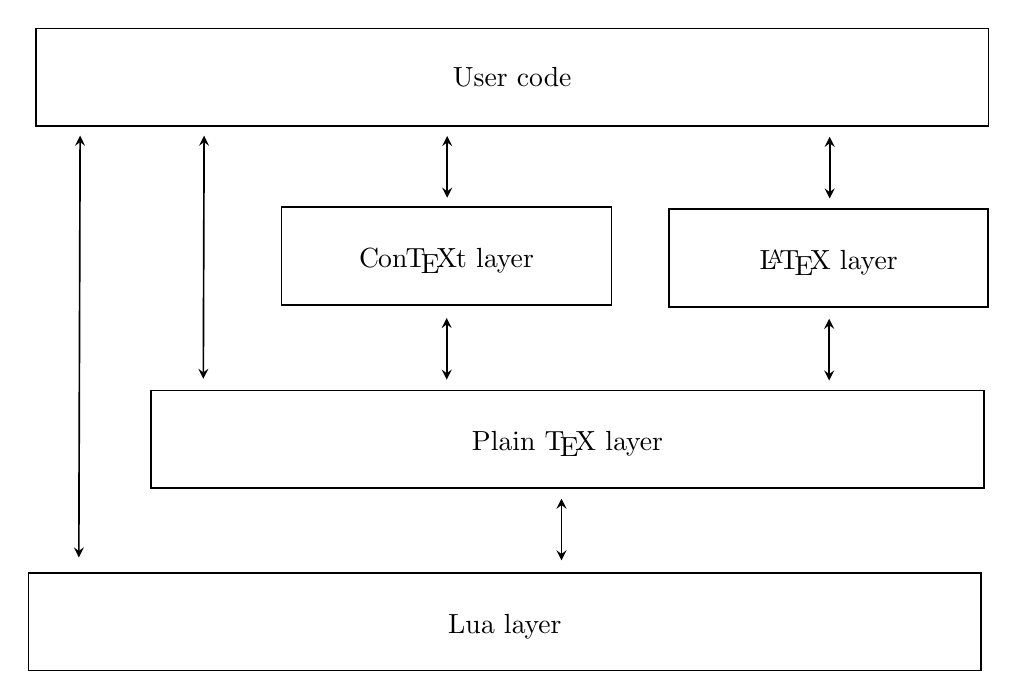
\begin{tikzpicture}
\pgftransformxscale{1.000000}
\pgftransformyscale{-1.23800}
\definecolor{dialinecolor}{rgb}{0.000000, 0.000000, 0.000000}
\pgfsetstrokecolor{dialinecolor}
\definecolor{dialinecolor}{rgb}{1.000000, 1.000000, 1.000000}
\pgfsetfillcolor{dialinecolor}
\definecolor{dialinecolor}{rgb}{1.000000, 1.000000, 1.000000}
\pgfsetfillcolor{dialinecolor}
\fill (4.282853\du,-3.750000\du)--(4.282853\du,-1.850000\du)--(11.971656\du,-1.850000\du)--(11.971656\du,-3.750000\du)--cycle;
\pgfsetlinewidth{0.040000\du}
\pgfsetdash{}{0pt}
\pgfsetdash{}{0pt}
\pgfsetmiterjoin
\definecolor{dialinecolor}{rgb}{0.000000, 0.000000, 0.000000}
\pgfsetstrokecolor{dialinecolor}
\draw (4.282853\du,-3.750000\du)--(4.282853\du,-1.850000\du)--(11.971656\du,-1.850000\du)--(11.971656\du,-3.750000\du)--cycle;
\definecolor{dialinecolor}{rgb}{0.000000, 0.000000, 0.000000}
\pgfsetstrokecolor{dialinecolor}
\node at (8.127254\du,-2.705000\du){\LaTeX{} layer};
\definecolor{dialinecolor}{rgb}{1.000000, 1.000000, 1.000000}
\pgfsetfillcolor{dialinecolor}
\fill (-5.055135\du,-3.788555\du)--(-5.055135\du,-1.888555\du)--(2.894865\du,-1.888555\du)--(2.894865\du,-3.788555\du)--cycle;
\pgfsetlinewidth{0.040000\du}
\pgfsetdash{}{0pt}
\pgfsetdash{}{0pt}
\pgfsetmiterjoin
\definecolor{dialinecolor}{rgb}{0.000000, 0.000000, 0.000000}
\pgfsetstrokecolor{dialinecolor}
\draw (-5.055135\du,-3.788555\du)--(-5.055135\du,-1.888555\du)--(2.894865\du,-1.888555\du)--(2.894865\du,-3.788555\du)--cycle;
\definecolor{dialinecolor}{rgb}{0.000000, 0.000000, 0.000000}
\pgfsetstrokecolor{dialinecolor}
\node at (-1.080135\du,-2.743555\du){\Hologo{ConTeXt} layer};
\definecolor{dialinecolor}{rgb}{1.000000, 1.000000, 1.000000}
\pgfsetfillcolor{dialinecolor}
\fill (-8.200000\du,-0.224996\du)--(-8.200000\du,1.675004\du)--(11.870000\du,1.675004\du)--(11.870000\du,-0.224996\du)--cycle;
\pgfsetlinewidth{0.040000\du}
\pgfsetdash{}{0pt}
\pgfsetdash{}{0pt}
\pgfsetmiterjoin
\definecolor{dialinecolor}{rgb}{0.000000, 0.000000, 0.000000}
\pgfsetstrokecolor{dialinecolor}
\draw (-8.200000\du,-0.224996\du)--(-8.200000\du,1.675004\du)--(11.870000\du,1.675004\du)--(11.870000\du,-0.224996\du)--cycle;
\definecolor{dialinecolor}{rgb}{0.000000, 0.000000, 0.000000}
\pgfsetstrokecolor{dialinecolor}
\node at (1.835000\du,0.820004\du){Plain \TeX{} layer};
\definecolor{dialinecolor}{rgb}{1.000000, 1.000000, 1.000000}
\pgfsetfillcolor{dialinecolor}
\fill (-11.150000\du,3.325006\du)--(-11.150000\du,5.225006\du)--(11.800000\du,5.225006\du)--(11.800000\du,3.325006\du)--cycle;
\pgfsetlinewidth{0.040000\du}
\pgfsetdash{}{0pt}
\pgfsetdash{}{0pt}
\pgfsetmiterjoin
\definecolor{dialinecolor}{rgb}{0.000000, 0.000000, 0.000000}
\pgfsetstrokecolor{dialinecolor}
\draw (-11.150000\du,3.325006\du)--(-11.150000\du,5.225006\du)--(11.800000\du,5.225006\du)--(11.800000\du,3.325006\du)--cycle;
\definecolor{dialinecolor}{rgb}{0.000000, 0.000000, 0.000000}
\pgfsetstrokecolor{dialinecolor}
\node at (0.325000\du,4.370006\du){Lua layer};
\pgfsetlinewidth{0.040000\du}
\pgfsetdash{}{0pt}
\pgfsetdash{}{0pt}
\pgfsetbuttcap
{
\definecolor{dialinecolor}{rgb}{0.000000, 0.000000, 0.000000}
\pgfsetfillcolor{dialinecolor}
\pgfsetarrowsstart{stealth}
\pgfsetarrowsend{stealth}
\definecolor{dialinecolor}{rgb}{0.000000, 0.000000, 0.000000}
\pgfsetstrokecolor{dialinecolor}
\draw (-9.906400\du,-5.181570\du)--(-9.937836\du,3.024193\du);
}
\pgfsetlinewidth{0.040000\du}
\pgfsetdash{}{0pt}
\pgfsetdash{}{0pt}
\pgfsetbuttcap
{
\definecolor{dialinecolor}{rgb}{0.000000, 0.000000, 0.000000}
\pgfsetfillcolor{dialinecolor}
\pgfsetarrowsstart{stealth}
\pgfsetarrowsend{stealth}
\definecolor{dialinecolor}{rgb}{0.000000, 0.000000, 0.000000}
\pgfsetstrokecolor{dialinecolor}
\draw (-6.919693\du,-5.181570\du)--(-6.938734\du,-0.450800\du);
}
\pgfsetlinewidth{0.040000\du}
\pgfsetdash{}{0pt}
\pgfsetdash{}{0pt}
\pgfsetbuttcap
{
\definecolor{dialinecolor}{rgb}{0.000000, 0.000000, 0.000000}
\pgfsetfillcolor{dialinecolor}
\pgfsetarrowsstart{stealth}
\pgfsetarrowsend{stealth}
\definecolor{dialinecolor}{rgb}{0.000000, 0.000000, 0.000000}
\pgfsetstrokecolor{dialinecolor}
\draw (-1.063746\du,-5.175791\du)--(-1.063746\du,-3.975793\du);
}
\definecolor{dialinecolor}{rgb}{1.000000, 1.000000, 1.000000}
\pgfsetfillcolor{dialinecolor}
\fill (-10.972500\du,-7.267480\du)--(-10.972500\du,-5.367480\du)--(11.977500\du,-5.367480\du)--(11.977500\du,-7.267480\du)--cycle;
\pgfsetlinewidth{0.040000\du}
\pgfsetdash{}{0pt}
\pgfsetdash{}{0pt}
\pgfsetmiterjoin
\definecolor{dialinecolor}{rgb}{0.000000, 0.000000, 0.000000}
\pgfsetstrokecolor{dialinecolor}
\draw (-10.972500\du,-7.267480\du)--(-10.972500\du,-5.367480\du)--(11.977500\du,-5.367480\du)--(11.977500\du,-7.267480\du)--cycle;
\definecolor{dialinecolor}{rgb}{0.000000, 0.000000, 0.000000}
\pgfsetstrokecolor{dialinecolor}
\node at (0.502500\du,-6.322480\du){User code};
\pgfsetlinewidth{0.040000\du}
\pgfsetdash{}{0pt}
\pgfsetdash{}{0pt}
\pgfsetbuttcap
{
\definecolor{dialinecolor}{rgb}{0.000000, 0.000000, 0.000000}
\pgfsetfillcolor{dialinecolor}
\pgfsetarrowsstart{stealth}
\pgfsetarrowsend{stealth}
\definecolor{dialinecolor}{rgb}{0.000000, 0.000000, 0.000000}
\pgfsetstrokecolor{dialinecolor}
\draw (8.149986\du,-5.159541\du)--(8.149986\du,-3.959543\du);
}
\pgfsetlinewidth{0.040000\du}
\pgfsetdash{}{0pt}
\pgfsetdash{}{0pt}
\pgfsetbuttcap
{
\definecolor{dialinecolor}{rgb}{0.000000, 0.000000, 0.000000}
\pgfsetfillcolor{dialinecolor}
\pgfsetarrowsstart{stealth}
\pgfsetarrowsend{stealth}
\definecolor{dialinecolor}{rgb}{0.000000, 0.000000, 0.000000}
\pgfsetstrokecolor{dialinecolor}
\draw (-1.074995\du,-1.634548\du)--(-1.074995\du,-0.434550\du);
}
\pgfsetlinewidth{0.040000\du}
\pgfsetdash{}{0pt}
\pgfsetdash{}{0pt}
\pgfsetbuttcap
{
\definecolor{dialinecolor}{rgb}{0.000000, 0.000000, 0.000000}
\pgfsetfillcolor{dialinecolor}
\pgfsetarrowsstart{stealth}
\pgfsetarrowsend{stealth}
\definecolor{dialinecolor}{rgb}{0.000000, 0.000000, 0.000000}
\pgfsetstrokecolor{dialinecolor}
\draw (8.138736\du,-1.618298\du)--(8.138736\du,-0.418300\du);
}
\pgfsetlinewidth{0.040000\du}
\pgfsetdash{}{0pt}
\pgfsetdash{}{0pt}
\pgfsetbuttcap
{
\definecolor{dialinecolor}{rgb}{0.000000, 0.000000, 0.000000}
\pgfsetfillcolor{dialinecolor}
\pgfsetarrowsstart{stealth}
\pgfsetarrowsend{stealth}
\definecolor{dialinecolor}{rgb}{0.000000, 0.000000, 0.000000}
\pgfsetstrokecolor{dialinecolor}
\draw (1.689638\du,1.881695\du)--(1.689638\du,3.081693\du);
}
\end{tikzpicture}
\endgroup
\end{filecontents}

% Set up the bibliography.
\begin{filecontents}[overwrite,nosearch,noheader]{markdown.bib}
@book{tantau21,
  author    = {Till Tantau and Joseph Wright and Vedran Miletić},
  title     = {The Beamer class},
  date      = {2021-02-10},
  url       = {https://mirrors.ctan.org/macros/latex/contrib/beamer/doc/beameruserguide.pdf},
  urldate   = {2021-02-11}}
@online{sotkov17,
  author    = {Sotkov, Anton},
  title     = {File transclusion syntax for Markdown},
  date      = {2017-01-19},
  url       = {https://github.com/iainc/Markdown-Content-Blocks},
  urldate   = {2018-01-08}}
@book{luatex17,
  author    = {{Lua\TeX{} development team}},
  title     = {Lua\TeX{} reference manual},
  year      = {2017},
  month     = {2},
  url       = {http://www.luatex.org/svn/trunk/manual/luatex.pdf},
  urldate   = {2018-01-08}}
@book{latex17,
  author    = {Braams, Johannes and Carlisle, David and Jeffrey, Alan and
               Lamport, Leslie and Mittelbach, Frank and Rowley, Chris and
               Schöpf, Rainer},
  title     = {The \Hologo{LaTeX2e} Sources},
  date      = {2017-04-15},
  url       = {https://mirrors.ctan.org/macros/latex/base/source2e.pdf},
  urldate   = {2018-01-08}}
@book{mittelbach17,
  author    = {Mittelbach, Frank},
  title     = {The \texttt{doc} and \texttt{shortvrb} Packages},
  date      = {2017-04-15},
  url       = {https://mirrors.ctan.org/macros/latex/base/doc.pdf},
  urldate   = {2018-02-19}}
@book{poore17,
  author    = {Poore, Geoffrey M.},
  title     = {The \texttt{minted} Package},
  subtitle  = {Highlighted source code in \LaTeX},
  date      = {2017-07-19},
  version   = {v2.5},
  url       = {https://mirrors.ctan.org/macros/latex/contrib/minted/minted.pdf},
  urldate   = {2020-09-01}}
@online{novotny15,
  author    = {Novotný, Vít},
  year      = {2015},
  title     = {TeXový interpret jazyka Markdown (markdown.sty)},
  location  = {Brno, Czech Republic},
  publisher = {Masaryk University},
  url       = {https://www.muni.cz/en/research/projects/32984},
  urldate   = {2018-02-19}}
@book{ierusalimschy13,
  author    = {Ierusalimschy, Roberto},
  year      = {2013},
  title     = {Programming in Lua},
  edition   = {3},
  isbn      = {978-85-903798-5-0},
  pagetotal = {xviii, 347},
  location  = {Rio de Janeiro},
  publisher = {PUC-Rio}}
@book{knuth86,
  author    = {Knuth, Donald Ervin},
  year      = {1986},
  title     = {The \TeX{}book},
  edition   = {3},
  isbn      = {0-201-13447-0},
  pagetotal = {ix, 479},
  publisher = {Addison-Wesley}}
@online{novotny21,
  author    = {Novotný, Vít},
  title     = {\Hologo{LaTeX2e} no longer keys packages by pathnames},
  date      = {2021-02-20},
  url       = {https://github.com/latex3/latex2e/issues/510},
  urldate   = {2021-02-21}}
\end{filecontents}
\usepackage[
  backend=biber,
  style=numeric,
  sorting=none,
  autolang=other,
  sortlocale=auto]{biblatex}
\addbibresource{markdown.bib}

\begin{document}
\printtitlepage
\tableofcontents
{\def\addcontentsline#1#2#3{}\listoffigures}
\DocInput{markdown.dtx}
\printbibliography[heading=bibintoc]
\printindex
\end{document}
%</driver>
%<*manual-css>

html {
  font-size: 100%;
  overflow-y: scroll;
  -webkit-text-size-adjust: 100%;
  -ms-text-size-adjust: 100%;
}

body {
  color: #444;
  font-family: Georgia, Palatino, 'Palatino Linotype', Times, 'Times New Roman', serif;
  font-size: 12px;
  line-height: 1.7;
  padding: 1em;
  margin: auto;
  max-width: 42em;
  background: #fefefe;
}

a {
  color: #0645ad;
}

a:visited {
  color: #0b0080;
}

a:hover {
  color: #06e;
}

a:active {
  color: #faa700;
}

a:focus {
  outline: thin dotted;
}

*::-moz-selection {
  background: rgba(255, 255, 0, 0.3);
  color: #000;
}

*::selection {
  background: rgba(255, 255, 0, 0.3);
  color: #000;
}

a::-moz-selection {
  background: rgba(255, 255, 0, 0.3);
  color: #0645ad;
}

a::selection {
  background: rgba(255, 255, 0, 0.3);
  color: #0645ad;
}

p {
  margin: 1em 0;
}

img {
  max-width: 100%;
}

h1, h2, h3, h4, h5, h6 {
  color: #111;
  line-height: 125%;
  margin-top: 2em;
  font-weight: normal;
}

h4, h5, h6 {
  font-weight: bold;
}

h1 {
  font-size: 2.5em;
}

h2 {
  font-size: 2em;
}

h3 {
  font-size: 1.5em;
}

h4 {
  font-size: 1.2em;
}

h5 {
  font-size: 1em;
}

h6 {
  font-size: 0.9em;
}

blockquote {
  color: #666666;
  margin: 0;
  padding-left: 3em;
  border-left: 0.5em #EEE solid;
}

hr {
  display: block;
  height: 2px;
  border: 0;
  border-top: 1px solid #aaa;
  border-bottom: 1px solid #eee;
  margin: 1em 0;
  padding: 0;
}

pre, code, kbd, samp {
  color: #000;
  font-family: monospace, monospace;
  _font-family: 'courier new', monospace;
  font-size: 0.98em;
}

pre {
  white-space: pre;
  white-space: pre-wrap;
  word-wrap: break-word;
}

b, strong {
  font-weight: bold;
}

dfn {
  font-style: italic;
}

ins {
  background: #ff9;
  color: #000;
  text-decoration: none;
}

mark {
  background: #ff0;
  color: #000;
  font-style: italic;
  font-weight: bold;
}

sub, sup {
  font-size: 75%;
  line-height: 0;
  position: relative;
  vertical-align: baseline;
}

sup {
  top: -0.5em;
}

sub {
  bottom: -0.25em;
}

ul, ol {
  margin: 1em 0;
  padding: 0 0 0 2em;
}

li p:last-child {
  margin-bottom: 0;
}

ul ul, ol ol {
  margin: .3em 0;
}

dl {
  margin-bottom: 1em;
}

dt {
  font-weight: bold;
  margin-bottom: .8em;
}

dd {
  margin: 0 0 .8em 2em;
}

dd:last-child {
  margin-bottom: 0;
}

img {
  border: 0;
  -ms-interpolation-mode: bicubic;
  vertical-align: middle;
}

figure {
  display: block;
  text-align: center;
  margin: 1em 0;
}

figure img {
  border: none;
  margin: 0 auto;
}

figcaption {
  font-size: 0.8em;
  font-style: italic;
  margin: 0 0 .8em;
}

table {
  margin-bottom: 2em;
  border-bottom: 1px solid #ddd;
  border-right: 1px solid #ddd;
  border-spacing: 0;
  border-collapse: collapse;
}

table th {
  padding: .2em 1em;
  background-color: #eee;
  border-top: 1px solid #ddd;
  border-left: 1px solid #ddd;
}

table td {
  padding: .2em 1em;
  border-top: 1px solid #ddd;
  border-left: 1px solid #ddd;
  vertical-align: top;
}

.author {
  font-size: 1.2em;
  text-align: center;
}

@media only screen and (min-width: 480px) {
  body {
    font-size: 14px;
  }
}
@media only screen and (min-width: 768px) {
  body {
    font-size: 16px;
  }
}
@media print {
  * {
    background: transparent !important;
    color: black !important;
    filter: none !important;
    -ms-filter: none !important;
  }

  body {
    font-size: 12pt;
    max-width: 100%;
  }

  a, a:visited {
    text-decoration: underline;
  }

  hr {
    height: 1px;
    border: 0;
    border-bottom: 1px solid black;
  }

  a[href]:after {
    content: " (" attr(href) ")";
  }

  abbr[title]:after {
    content: " (" attr(title) ")";
  }

  .ir a:after, a[href^="javascript:"]:after, a[href^="#"]:after {
    content: "";
  }

  pre, blockquote {
    border: 1px solid #999;
    padding-right: 1em;
    page-break-inside: avoid;
  }

  tr, img {
    page-break-inside: avoid;
  }

  img {
    max-width: 100% !important;
  }

  @page :left {
    margin: 15mm 20mm 15mm 10mm;
}

  @page :right {
    margin: 15mm 10mm 15mm 20mm;
}

  p, h2, h3 {
    orphans: 3;
    widows: 3;
  }

  h2, h3 {
    page-break-after: avoid;
  }
}

.tex sub, .latex sub, .latex sup {
  text-transform: uppercase;
}

.tex sub, .latex sub {
  vertical-align: -0.1ex;
  margin-left: -0.1667em;
  margin-right: -0.125em;
}

.tex, .latex, .tex sub, .latex sub {
  font-size: 1em;
}

.latex sup {
  font-size: 0.85em;
  vertical-align: -0.35em;
  margin-left: -0.36em;
  margin-right: -0.15em;
}

abbr {
  text-transform: lowercase;
  font-variant: small-caps;
}

%</manual-css>
%<*manual>

---
title:  Markdown Package User Manual
author: Vít Novotný
date:   \markdownVersion{} (\markdownLastModified{})
---

% \fi
% \par
% \begin{markdown}

<link href="https://afeld.github.io/emoji-css/emoji.css" rel="stylesheet" />

Introduction
============
The [Markdown package][pkg] converts [markdown][] markup to \TeX{} commands. The
functionality is provided both as a Lua module and as plain \TeX{}, \LaTeX{}, and
\Hologo{ConTeXt} macro packages that can be used to directly typeset \TeX documents
containing markdown markup. Unlike other convertors, the Markdown package
does not require any external programs, and makes it easy to redefine how each
and every markdown element is rendered.  Creative abuse of the markdown
syntax is encouraged. 😉

 [markdown]: https://daringfireball.net/projects/markdown/basics
             (Daring Fireball: Markdown Basics)
 [pkg]:      https://ctan.org/pkg/markdown
             (CTAN: Package markdown)

% This document is a technical documentation for the \pkg{Markdown} package. It
% consists of three sections. This section introduces the package and outlines
% its prerequisites. Section \vref{sec:interfaces} describes the interfaces
% exposed by the package. Section \vref{sec:implementation} describes the
% implementation of the package. The technical documentation contains only a
% limited number of tutorials and code examples. You can find more of these in
% the [user manual.][manual]
%
%  [manual]: http://mirrors.ctan.org/macros/generic/markdown/markdown.html
%
% \end{markdown}
% \iffalse

This document is a user manual for the [Markdown package][pkg]. It provides
tutorials and code examples. For an in-depth description of the package
requirements, interfaces, and implementation, please refer to the [technical
documentation][techdoc].

 [techdoc]: http://mirrors.ctan.org/macros/generic/markdown/markdown.pdf
            (A Markdown Interpreter for TeX)

%</manual>
%<*lua,lua-cli>
% \fi
%  \begin{macrocode}
local metadata = {
    version   = "$(VERSION)",
    comment   = "A module for the conversion from markdown to plain TeX",
    author    = "John MacFarlane, Hans Hagen, Vít Novotný",
    copyright = {"2009-2016 John MacFarlane, Hans Hagen",
                 "2016-2021 Vít Novotný"},
    license   = "LPPL 1.3c"
}

%    \end{macrocode}
% \iffalse
%</lua,lua-cli>
%<*lua>
% \fi
%  \begin{macrocode}
if not modules then modules = { } end
modules['markdown'] = metadata
%    \end{macrocode}
% \iffalse
%</lua>
%<*manual>

Requirements
------------

The package requires either [our official Docker image][docker], which contains
the latest development version of the Markdown package, or a \TeX{}
distribution: [\TeX{} Live][tl] ≥ 2013 is known to work and so are recent
versions of [Mik\TeX{}][mik]. If you are using a minimal installation of a
\TeX{} distribution, please consult the [technical documentation][techdoc] for
a detailed list of required packages.

 [docker]: https://hub.docker.com/r/witiko/markdown/tags (witiko/markdown - Docker Image)
 [tl]: https://www.tug.org/texlive/ (TeX Live - TeX Users Group)
 [mik]: https://miktex.org/ (Home - MiKTeXorg)

Installation
------------

If you are using an older \TeX{} distribution such as [\TeX{} Live][tl] < 2016,
you will need to install the Markdown package.

First, download the package from the repository using Git:
``` sh
git clone https://github.com/witiko/markdown
``````
Next, enter the directory named `markdown` and interpret the file named
`markdown.ins` file using a Unicode-aware \TeX{} engine, such as XeTeX or
LuaTeX:
``` sh
cd markdown
luatex markdown.ins
``````
This should produce the following files:

 * `markdown.lua`, the Lua module,
 * `markdown-cli.lua`, the Lua command-line interface,
 * `markdown.tex`, the plain \TeX{} macro package,
 * `markdown.sty`, the \LaTeX{} package,
 * `markdownthemewitiko_dot.sty`, the `witiko/dot` \LaTeX{} theme,
 * `markdownthemewitiko_graphicx_http.sty`, the `witiko/graphicx/http` \LaTeX{} theme,
 * `markdownthemewitiko_tilde.sty`, the `witiko/tilde` \LaTeX{} theme, and
 * `t-markdown.tex`, the \Hologo{ConTeXt} module.

### Local Installation

To perform a local installation, place the above files into your \TeX{}
directory structure. This is generally where the individual files should be
placed:

 * `⟨TEXMF⟩/tex/luatex/markdown/markdown.lua`
 * `⟨TEXMF⟩/scripts/markdown/markdown-cli.lua`
 * `⟨TEXMF⟩/tex/generic/markdown/markdown.tex`
 * `⟨TEXMF⟩/tex/latex/markdown/markdown.sty`
 * `⟨TEXMF⟩/tex/latex/markdown/markdownthemewitiko_dot.sty`
 * `⟨TEXMF⟩/tex/latex/markdown/markdownthemewitiko_graphicx_http.sty`
 * `⟨TEXMF⟩/tex/latex/markdown/markdownthemewitiko_tilde.sty`
 * `⟨TEXMF⟩/tex/context/third/markdown/t-markdown.tex`

where `⟨TEXMF⟩` corresponds to a root of your \TeX{} distribution, such as
`/usr/share/texmf` and `~/texmf` on UN\*X systems or
`C:\Users\`\meta{Your username}`\texmf` on Windows systems. When in doubt,
consult the manual of your \TeX{} distribution.

### Portable Installation

Alternatively, you can also store the above files in the same folder as your
\TeX{} document and distribute them together. This way your document can be
portably typeset on legacy \TeX{} distributions.

Since Markdown version 2.10.0, the file `markdown.tex` must be placed in
a directory named `markdown` due to [issue #74][issue-74].

 [issue-74]: https://github.com/witiko/markdown/issues/74 (Does not compile if user names own document markdown.tex)

%</manual>
%<*lua>
% \fi
% \par
% \begin{markdown}
%
% Requirements
%-------------
%
% This section gives an overview of all resources required by the package.
%
%### Lua Requirements
% \label{sec:luaprerequisites}
% The Lua part of the package requires that the following Lua modules are
% available from within the Lua\TeX{} engine:
%
% \pkg{LPeg${}\geq{}$0.10}
%
%:    A pattern-matching library for the writing of recursive descent parsers
%     via the Parsing Expression Grammars (\acro{peg}s). It is used by the
%     \pkg{Lunamark} library to parse the markdown input.
%     \pkg{LPeg${}\geq{}$0.10} is included in Lua\TeX${}\geq{}$0.72.0 (\TeX
%     Live${}\geq{}2013$).
%
% \end{markdown}
%  \begin{macrocode}
local lpeg = require("lpeg")
%    \end{macrocode}
% \par
% \begin{markdown}
%
% \pkg{Selene Unicode}
%
%:    A library that provides support for the processing of wide strings. It is
%     used by the \pkg{Lunamark} library to cast image, link, and footnote tags
%     to the lower case. \pkg{Selene Unicode} is included in all releases of
%     Lua\TeX{} (\TeX Live${}\geq{}2008$).
%
% \end{markdown}
%  \begin{macrocode}
local ran_ok, unicode = pcall(require, "unicode")
%    \end{macrocode}
% \begin{markdown}
%
% If the Selene Unicode library is unavailable and we are using
% Lua${}\geq{}$5.3, we will use the built-in support for Unicode.
%
% \end{markdown}
%  \begin{macrocode}
if not ran_ok then
  unicode = {["utf8"]={char=utf8.char}}
end
%    \end{macrocode}
% \par
% \begin{markdown}
%
% \pkg{MD5}
%
%:    A library that provides \acro{md5} crypto functions. It is used by the
%     \pkg{Lunamark} library to compute the digest of the input for caching
%     purposes. \pkg{MD5} is included in all releases of Lua\TeX{} (\TeX
%     Live${}\geq{}2008$).
%
% \end{markdown}
%  \begin{macrocode}
local md5 = require("md5")
%    \end{macrocode}
% \par
% \begin{markdown}
%
% All the abovelisted modules are statically linked into the current version of
% the Lua\TeX{} engine~[@luatex17, Section 3.3].
%
% \end{markdown}
% \iffalse
%</lua>
%<*tex>
% \fi
% \par
% \begin{markdown}
%
%### Plain \TeX{} Requirements
% \label{sec:texprerequisites}
% The plain \TeX{} part of the package requires that the plain \TeX{}
% format (or its superset) is loaded, all the Lua prerequisites (see
% Section \vref{sec:luaprerequisites}), and the following Lua module:
%
% \pkg{Lua File System}
%
%:    A library that provides access to the filesystem via \acro{os}-specific
%     syscalls. It is used by the plain \TeX{} code to create the cache
%     directory specified by the \m{markdownOptionCacheDir} macro before
%     interfacing with the \pkg{Lunamark} library. \pkg{Lua File System} is
%     included in all releases of Lua\TeX{} (\TeX Live${}\geq{}2008$).
%
%     The plain \TeX{} code makes use of the \luam{isdir} method that was added
%     to the \pkg{Lua File System} library by the Lua\TeX{} engine
%     developers~[@luatex17, Section 3.2].
%
% The \pkg{Lua File System} module is statically linked into the Lua\TeX{}
% engine~[@luatex17, Section~3.3].
%
% Unless you convert markdown documents to \TeX{} manually using the Lua
% command-line interface (see Section \vref{sec:lua-cli-interface}), the plain
% \TeX{} part of the package will require that either the Lua\TeX{}
% \m{directlua} primitive or the shell access file stream 18 is available in
% your \TeX{} engine. If only the shell access file stream is available in your
% \TeX{} engine (as is the case with \hologo{pdfTeX} and \Hologo{XeTeX}) or if
% you enforce the use of shell using the \m{markdownMode} macro, then unless
% your \TeX{} engine is globally configured to enable shell access, you will
% need to provide the `-shell-escape` parameter to your engine when typesetting
% a document.
%
% \end{markdown}
% \iffalse
%</tex>
%<*latex>
% \fi
% \par
% \begin{markdown}
%
%### \LaTeX{} Requirements
% \label{sec:latexprerequisites}
% The \LaTeX{} part of the package requires that the \Hologo{LaTeX2e} format is
% loaded,
% \end{markdown}
% \iffalse
%<*latex-themes-witiko-dot,latex-themes-witiko-graphicx-http,latex-themes-witiko-tilde>
% \fi
%  \begin{macrocode}
\NeedsTeXFormat{LaTeX2e}%
%    \end{macrocode}
% \iffalse
%</latex-themes-witiko-dot,latex-themes-witiko-graphicx-http,latex-themes-witiko-tilde>
% \fi
% \begin{markdown}
% a \TeX{} engine that extends \Hologo{eTeX}, all the plain \TeX{}
% prerequisites (see Section \vref{sec:texprerequisites}), and the following
% \Hologo{LaTeX2e} packages:
%
% \pkg{keyval}
%
%:    A package that enables the creation of parameter sets. This package is
%     used to provide the \m{markdownSetup} macro, the package options
%     processing, as well as the parameters of the \envm{markdown*} \LaTeX{}
%     environment.
%
% \end{markdown}
%  \begin{macrocode}
\RequirePackage{keyval}
%    \end{macrocode}
% \par
% \begin{markdown}
%
% \pkg{xstring}
%
%:    A package that provides useful macros for manipulating strings of tokens.
%
% \end{markdown}
%  \begin{macrocode}
\RequirePackage{xstring}
%    \end{macrocode}
% \par
% \begin{markdown}
%
% The following packages are soft prerequisites. They are only used to provide
% default token renderer prototype (see Section
% \vref{sec:texrendererprototypes}) and will not be loaded if the `plain`
% package option has been enabled (see Section \vref{sec:latexplain}):
%
% \pkg{url}
%
%:    A package that provides the \m{url} macro for the typesetting of
%     links.
%
% \pkg{graphicx}
%
%:    A package that provides the \m{includegraphics} macro for the typesetting
%     of images.
%
% \pkg{paralist}
%
%:    A package that provides the \envm{compactitem}, \envm{compactenum}, and
%     \envm{compactdesc} macros for the typesetting of tight bulleted lists,
%     ordered lists, and definition lists.
%
% \pkg{ifthen}
%
%:    A package that provides a concise syntax for the inspection of macro
%     values. It is used to determine whether or not the \pkg{paralist} package
%     should be loaded based on the user options, in the `witiko/dot` \LaTeX{}
%     theme (see Section \vref{sec:latexthemes}), and to provide default token
%     renderer prototypes.
%
% \pkg{fancyvrb}
%
%:    A package that provides the \m{VerbatimInput} macros for the verbatim
%     inclusion of files containing code.
%
% \pkg{csvsimple}
%
%:    A package that provides the \m{csvautotabular} macro for typesetting
%     \acro{csv} files.
%
% \pkg{gobble}
%
%:    A package that provides the \m{\@gobblethree} \TeX{} command that
%     is used in the default renderer prototype for citations.
%
% \pkg{amsmath} and \pkg{amssymb}
%
%:    Packages that provide symbols used for drawing ticked and unticked
%     boxes.
%
% \end{markdown}
% \iffalse
%</latex>
%<*context>
% \fi
% \par
% \begin{markdown}
%
%### \Hologo{ConTeXt} Prerequisites
% The \Hologo{ConTeXt} part of the package requires that either the Mark II or
% the Mark IV format is loaded, all the plain \TeX{} prerequisites (see
% Section \vref{sec:texprerequisites}), and the following \Hologo{ConTeXt}
% modules:
%
% \pkg{m-database}
%
%:    A module that provides the default token renderer prototype for
%     iA\,Writer content blocks with the \acro{csv} filename extension (see
%     Section \vref{sec:texrendererprototypes}).
%
% Feedback
%---------
% Please use the \pkg{Markdown} project page on
% [GitHub](https://github.com/witiko/markdown/issues) to report bugs and submit
% feature requests. If you do not want to report a bug or request a feature but
% are simply in need of assistance, you might want to consider posting your
% question to the [\TeX-\LaTeX{} Stack Exchange.](https://tex.stackexchange.com)
% community question answering web site under the `markdown` tag.
%
% Acknowledgements
%-----------------
% The Lunamark Lua module provides speedy markdown parsing for the package. I
% would like to thank John Macfarlane, the creator of Lunamark, for releasing
% Lunamark under a permissive license, which enabled its use in the Markdown
% package.
%
% Extensive user documentation for the Markdown package was kindly written by
% Lian Tze Lim and published by Overleaf.
%
% Funding by the the Faculty of Informatics at the Masaryk~University
% in~Brno~[@novotny15] is gratefully acknowledged.
%
% Support for content slicing (Lua options \Opt{shiftHeadings} and \Opt{slice})
% and pipe tables (Lua options \Opt{pipeTables} and \Opt{tableCaptions}) was
% graciously sponsored by David Vins and Omedym.
%
% The \TeX{} implementation of the package draws inspiration from several
% sources including the source code of \Hologo{LaTeX2e}, the \pkg{minted}
% package by Geoffrey M. Poore, which likewise tackles the issue of
% interfacing with an external interpreter from \TeX{}, the \pkg{filecontents}
% package by Scott Pakin and others.
%
% Interfaces
%===========
% \label{sec:interfaces}
% This part of the documentation describes the interfaces exposed by the package
% along with usage notes and examples. It is aimed at the user of the package.
%
% Since neither \TeX{} nor Lua provide interfaces as a language construct, the
% separation to interfaces and implementations is a *gentlemen's agreement*. It
% serves as a means of structuring this documentation and as a promise to the
% user that if they only access the package through the interface, the future
% minor versions of the package should remain backwards compatible.
%
% Figure \vref{fig:block-diagram} shows the high-level structure of the Markdown
% package: The translation from markdown to \TeX{} *token renderers* is exposed
% by the Lua layer. The plain \TeX{} layer exposes the conversion capabilities
% of Lua as \TeX{} macros. The \LaTeX{} and \Hologo{ConTeXt} layers provide
% syntactic sugar on top of plain \TeX{} macros. The user can interface with
% any and all layers.
%
% \end{markdown}
% \begin{figure}
% \centering
% \input markdown-figure-block-diagram
% \caption{A block diagram of the \pkg{Markdown} package}
% \label{fig:block-diagram}
% \end{figure}
% \iffalse
%</context>
%<*manual>

First Document
--------------

In this section, we will take the necessary steps to typeset our first markdown
document in \TeX{}. This will serve as our first hands-on experience with the
package and also as a reassurance that the package has been correctly installed.

If you are using [our official Docker image][docker], you need to prefix all
commands in this section with `docker run --rm -v "$PWD"/workdir:/workdir -w
/workdir witiko/markdown`. For example, instead of `luatex document.tex`, you
would execute the following command:
``` sh
docker run --rm -v "$PWD"/workdir:/workdir -w /workdir witiko/markdown \
  luatex document.tex
``````

### Using Lua

Using a text editor, create a text document named `document.tex` with the
following content:
``` tex
\input markdown
\input hello
\bye
```````

#### Using the Lua Module

Using a text editor, create a text document named `hello.lua` with the
following content:
``` lua
#!/usr/bin/env texlua
local ran_ok, kpse = pcall(require, "kpse")
if ran_ok then kpse.set_program_name("luatex") end
local markdown = require("markdown")
local convert = markdown.new()
print(convert("Hello *world*!"))
```````
Next, invoke LuaTeX from the terminal:
``` sh
texlua hello.lua > hello.tex
luatex document.tex
``````
A PDF document named `document.pdf` should be produced and contain the text
“Hello *world*!” Invoking pdfTeX should have the same effect:
``` sh
texlua hello.lua > hello.tex
pdftex document.tex
``````

#### Using the Lua Command-Line Interface

Using a text editor, create a text document named `hello.md` with the
following content:
``` md
Hello *world*!
``````
Next, invoke LuaTeX from the terminal:
``` sh
texlua ⟨CLI pathname⟩ -- hello.md hello.tex
luatex document.tex
``````
where \meta{CLI pathname} corresponds to the location of the Lua CLI script file,
such as `~/texmf/scripts/markdown/markdown-cli.lua` on UN\*X systems or
`C:\Users\`\meta{Your username}`\texmf\scripts\markdown\markdown-cli.lua` on Windows
systems. Use the command `kpsewhich -a markdown-cli.lua` to locate the Lua CLI
script file using [Kpathsea][].

 [Kpathsea]: https://tug.org/kpathsea/ (Kpathsea - TeX Users Group)

A PDF document named `document.pdf` should be produced and contain the text “Hello
*world*!” Invoking pdfTeX should have the same effect:
``` sh
texlua ⟨CLI pathname⟩ -- hello.md hello.tex
pdftex document.tex
``````

### Using Plain \TeX{}

Using a text editor, create a text document named `document.tex` with the
following content:
``` tex
\input markdown
\markdownBegin
Hello *world*!
\markdownEnd
\bye
```````
Next, invoke LuaTeX from the terminal:
``` sh
luatex document.tex
``````
A PDF document named `document.pdf` should be produced and contain the text
“Hello *world*!” Invoking pdfTeX should have the same effect:
``` sh
pdftex --shell-escape document.tex
```````

### Using \LaTeX{}

Using a text editor, create a text document named `document.tex` with the
following content:
``` tex
\documentclass{article}
\usepackage{markdown}
\begin{document}
\begin{markdown}
Hello *world*!
\end{markdown}
\end{document}
```````
Next, invoke LuaTeX from the terminal:
``` sh
lualatex document.tex
``````
A PDF document named `document.pdf` should be produced and contain the text “Hello
*world*!” Invoking pdfTeX should have the same effect:
``` sh
pdflatex --shell-escape document.tex
``````

***

As the next step, try typesetting the example documents distributed along with
the Markdown package:
``` sh
git clone https://github.com/witiko/markdown
cd markdown/examples
lualatex latex.tex
``````
A PDF document named `latex.pdf` should be produced. Open the text documents
`latex.tex` and `example.md` in a text editor to see how the example documents
are structured. Try changing the documents and typesetting them as follows:
``` sh
lualatex latex.tex
``````
to see the effect of your changes.

### Using \Hologo{ConTeXt}

Using a text editor, create a text document named `document.tex` with the
following content:
``` tex
\usemodule[t][markdown]
\starttext
\startmarkdown
Hello *world*!
\stopmarkdown
\stoptext
```````
Next, invoke LuaTeX from the terminal:
``` sh
context document.tex
``````
A PDF document named `document.pdf` should be produced and contain the text “Hello
*world*!” Invoking pdfTeX should have the same effect:
``` sh
texexec --passon=--shell-escape document.tex
``````

***

As the next step, try typesetting the example documents distributed along with
the Markdown package:
``` sh
git clone https://github.com/witiko/markdown
cd markdown/examples
context context.tex
``````
A PDF document named `context.pdf` should be produced. Open the text documents
`context.tex` and `example.md` in a text editor to see how the example documents
are structured. Try changing the documents and typesetting them as follows:
``` sh
context context.tex
``````
to see the effect of your changes.

Examples
========

In this section, I will describe the individual parts of the Markdown package.
Each part will be shown by example, leaving the implementation details to the
[technical documentation][techdoc].

 [techdoc]: https://mirrors.ctan.org/macros/generic/markdown/markdown.pdf
            (A Markdown Interpreter for \TeX{})

/markdown-interfaces.md
/markdown-options.md
/markdown-tokens.md

%</manual>
%<*lua>
% \fi
% \par
% \begin{markdown}
%
% Lua Interface
%--------------
% \label{sec:luainterface}
%
% \iffalse
%</lua>
%<*manual-interfaces>

Interfaces
----------

In this section, I will describe the individual interfaces exposed by the
Markdown package starting with the low-level Lua interfaces and all the way up
to the \LaTeX{} and \Hologo{ConTeXt} interfaces intended for the ordinary
user.

### Lua

The Lua programming language is what drives the conversion from markdown to
\TeX{} in the Markdown package. Based on the [Lunamark][] Lua library by John
MacFarlane, the Lua implementation is largely independent on \TeX{}, and can be
used separately from typesetting a document. Lua provides two interfaces: a Lua
module and a command-line interface (CLI).

 [Lunamark]: https://github.com/jgm/lunamark
             (Lua library for conversion between markup formats)

%</manual-interfaces>
%<*lua>
% \fi
%
% The Lua interface provides the conversion from \acro{utf}-\oldstylenums8
% encoded markdown to plain \TeX{}. This interface is used by the plain \TeX{}
% implementation (see Section \vref{sec:teximplementation}) and will be of
% interest to the developers of other packages and Lua modules.
%
% The Lua interface is implemented by the `markdown` Lua module.
%
% \end{markdown}
%  \begin{macrocode}
local M = {metadata = metadata}
%    \end{macrocode}
% \par
% \begin{markdown}
%
%### Conversion from Markdown to Plain \TeX{}
% \label{sec:luaconversion}
% The Lua interface exposes the \luamdef{new}`(options)` method.  This
% method creates converter functions that perform the conversion from markdown
% to plain \TeX{} according to the table `options` that contains options
% recognized by the Lua interface.  (see Section \vref{sec:luaoptions}). The
% `options` parameter is optional; when unspecified, the behaviour will be
% the same as if `options` were an empty table.
%
% The following example Lua code converts the markdown string `Hello
% *world*!` to a \TeX{} output using the default options and prints the \TeX{}
% output:
% ``` lua
% local md = require("markdown")
% local convert = md.new()
% print(convert("Hello *world*!"))
% ```````
%
% \end{markdown}
% \iffalse
%</lua>
%<*manual-interfaces>

#### Lua Module

A Lua module is a software library that can be used from in other programs.
The `markdown` Lua module makes it possible to convert markdown to \TeX{} from
within Lua\TeX{} documents and Lua scripts.

The `markdown` Lua module exposes the `new(`\meta{options}`)` method, which
creates a converter function from markdown to \TeX{}. The properties of the
converter function are specified by the Lua table `options`. The parameter is
optional; when unspecified, the behaviour will be the same as if \meta{options}
were an empty table.

Using a text editor, create a text document named `document.tex` with the
following content:
``` tex
\input markdown
\input lmfonts
\input example
\bye
```````
Using a text editor, create a text document named `example.lua` with the
following content:
``` lua
#!/usr/bin/env texlua
local ran_ok, kpse = pcall(require, "kpse")
if ran_ok then kpse.set_program_name("luatex") end
local markdown = require("markdown")
local input, convert_safe, convert_unsafe, paragraph

input = [[$\sqrt{-1}$ *equals* $i$.]]
convert_safe = markdown.new()
convert_unsafe = markdown.new({hybrid = true})
paragraph = [[\par]]

print(
  convert_safe(input) .. paragraph ..
  convert_unsafe(input)
)
```````
Next, invoke LuaTeX from the terminal:
``` sh
texlua example.lua > example.tex
luatex document.tex
``````
A PDF document named `document.pdf` should be produced and contain the
following text:

> \$\\sqrt{-1}\$ *equals* \$i\$.
> 
> √-̅1̅ *equals* $i$.

Invoking pdfTeX should have the same effect:
``` sh
texlua example.lua > example.tex
pdftex document.tex
``````

***

Rather than use the `texlua` interpreter, we can also access the `markdown` Lua
module directly from our document. Using a text editor, create a text document
named `document.tex` with the following content:
``` tex
\input markdown
\input lmfonts
\directlua{
  local markdown = require("markdown")
  local input, convert_safe, convert_unsafe, paragraph

  input = [[$\string\sqrt{-1}$ *equals* $i$.]]
  convert_safe = markdown.new()
  convert_unsafe = markdown.new({hybrid = true})
  paragraph = [[\par]]

  tex.sprint(
    convert_safe(input) .. paragraph ..
    convert_unsafe(input)
  )
}
\bye
```````
Next, invoke LuaTeX from the terminal:
``` sh
luatex document.tex
```````
A PDF document named `document.pdf` should be produced and contain the
following text:

> \$\\sqrt{-1}\$ *equals* \$i\$.
> 
> √-̅1̅ *equals* $i$.

In this case, we cannot use pdfTeX, because pdfTeX does not define the
`\directlua` \TeX{} command.

#### Lua Command-Line Interface

The Lua command-line interface (CLI) of the Markdown package makes the
functionality of the Lua module accessible from the command line.  This makes
it possible to convert documents from markdown to \TeX{} manually without any
knowledge of the Lua programming language.

The Lua command-line interface accepts the same options as the `markdown` Lua
module, but now the options are specified as command-line parameters.

Using a text editor, create a text document named `document.tex` with the
following content:
``` tex
\input markdown
\input lmfonts
\input safe

\begingroup
\catcode`\%=12
\input unsafe
\endgroup
\bye
```````
Using a text editor, create a text document named `example.md` with the
following content:
``` md
$\sqrt{-1}$ *equals* $i$.
``````
Next, invoke LuaTeX from the terminal:
``` sh
texlua ⟨CLI pathname⟩ -- example.md safe.tex
texlua ⟨CLI pathname⟩ hybrid=true -- example.md unsafe.tex
luatex document.tex
``````
where \meta{CLI pathname} corresponds to the location of the Lua CLI script file,
such as `~/texmf/scripts/markdown/markdown-cli.lua` on UN\*X systems or
`C:\Users\`\meta{Your username}`\texmf\scripts\markdown\markdown-cli.lua` on Windows
systems. Use the command `kpsewhich -a markdown-cli.lua` to locate the Lua CLI
script file using [Kpathsea][].

A PDF document named `document.pdf` should be produced and contain the
following text:

> \$\\sqrt{-1}\$ *equals* \$i\$.
> 
> √-̅1̅ *equals* $i$.

Invoking pdfTeX should have the same effect:
``` sh
texlua ⟨CLI pathname⟩ -- example.md safe.tex
texlua ⟨CLI pathname⟩ hybrid=true -- example.md unsafe.tex
pdftex document.tex
``````

%</manual-interfaces>
%<*lua>
% \fi
% \begin{markdown}
%
%### Options
% \label{sec:luaoptions}
% The Lua interface recognizes the following options. When unspecified, the
% value of a key is taken from the \luamdef{defaultOptions} table.
%
% \end{markdown}
% \iffalse
%</lua>
%<*manual-options>

## Options

In this section, I will describe all the options recognized by the Markdown
package.

%</manual-options>
%<*lua,lua-cli>
% \fi
%  \begin{macrocode}
local defaultOptions = {}
%    \end{macrocode}
% \begingroup
% \markdownSetup{
%   renderers = {
%     dlBegin = {\begin{optionlist}},
%     dlItem = {
%       #1
%       \begingroup
%       \markdownSetup{
%         renderers = {
%           dlBegin = {
%             \begingroup
%             \markdownSetup{
%               renderers = {
%                 dlItem = {\item[####1]},
%                 dlItemEnd = {}}}
%             \begin{valuelist}},
%           dlEnd = {
%             \end{valuelist}
%             \endgroup}}}},
%     dlItemEnd = {\endgroup},
%     dlEnd = {\end{optionlist}}}}
% \par
% \iffalse
%</lua,lua-cli>
%<*manual-options>

### Lua

Lua options control the conversion from markdown to \TeX{}. They are supported
by all interfaces of the Markdown package starting with the low-level Lua
interfaces and all the way up to the \LaTeX{} and \Hologo{ConTeXt} interfaces.

% \fi
% \begin{markdown}
% 
%### File and Directory Names
% 
% \end{markdown}
% \par
% \iffalse

#### Option `cacheDir`

`cacheDir` (default value: `"."`)

% \fi
% \begin{markdown}
%
% \Valitem[.]{cacheDir}{path}
%
:    A path to the directory containing auxiliary cache files. If the last
     segment of the path does not exist, it will be created by the Lua
     command-line and plain \TeX{} implementations. The Lua implementation
     expects that the entire path already exists.

     When iteratively writing and typesetting a markdown document, the cache
     files are going to accumulate over time. You are advised to clean the
     cache directory every now and then, or to set it to a temporary filesystem
     (such as `/tmp` on UN*X systems), which gets periodically emptied.

% \end{markdown}
% \iffalse

##### Lua Module Example {.unnumbered}

Using a text editor, create a text document named `document.tex` with the
following content:
``` tex
\input markdown
\directlua{
  local markdown = require("markdown")
  local convert = markdown.new({cacheDir = "cache"})
  local input = "Hello *world*!"
  tex.sprint(convert(input)) }
\bye
```````
Create an empty directory named `cache` next to our text document. Then, invoke
LuaTeX from the terminal:
``` sh
luatex document.tex
```````
A PDF document named `document.pdf` should be produced and contain the text
“Hello *world*!” Several cache files of the Markdown package will also be
produced in the `cache` directory as we requested using the `cacheDir` option.

##### Lua CLI Example {.unnumbered}

Using a text editor, create a text document named `document.tex` with the
following content:
``` tex
\input markdown
\input hello
\bye
```````
Using a text editor, create a text document named `hello.md` with the
following content:
``` md
Hello *world*!
``````
Next, invoke LuaTeX from the terminal:
``` sh
texlua ⟨CLI pathname⟩ cacheDir=cache -- hello.md hello.tex
luatex document.tex
```````
where \meta{CLI pathname} corresponds to the location of the Lua CLI script file,
such as `~/texmf/scripts/markdown/markdown-cli.lua` on UN\*X systems or
`C:\Users\`\meta{Your username}`\texmf\scripts\markdown\markdown-cli.lua` on Windows
systems. Use the command `kpsewhich -a markdown-cli.lua` to locate the Lua CLI
script file using [Kpathsea][].

A PDF document named `document.pdf` should be produced and contain the text
“Hello *world*!” A directory named `cache` containing several cache files of
the Markdown package will also be produced as we requested using the `cacheDir`
option.

##### Plain \TeX{} Example {.unnumbered}

Using a text editor, create a text document named `document.tex` with the
following content:
``` tex
\input markdown
\def\markdownOptionCacheDir{cache}
\markdownBegin
Hello *world*!
\markdownEnd
\bye
```````
Next, invoke LuaTeX from the terminal:
``` sh
luatex document.tex
``````
A PDF document named `document.pdf` should be produced and contain the text “Hello
*world*!” A directory named `cache` containing several cache files of the
Markdown package will also be produced as we requested using the `cacheDir`
option.

##### \LaTeX{} Example {.unnumbered}

Using a text editor, create a text document named `document.tex` with the
following content:
``` tex
\documentclass{article}
\usepackage[cacheDir=cache]{markdown}
\begin{document}
\begin{markdown}
Hello *world*!
\end{markdown}
\end{document}
```````
Next, invoke LuaTeX from the terminal:
``` sh
lualatex document.tex
``````
A PDF document named `document.pdf` should be produced and contain the text “Hello
*world*!” A directory named `cache` containing several cache files of the
Markdown package will also be produced as we requested using the `cacheDir`
option.

##### \Hologo{ConTeXt} Example {.unnumbered}

Using a text editor, create a text document named `document.tex` with the
following content:
``` tex
\usemodule[t][markdown]
\def\markdownOptionCacheDir{cache}
\starttext
\startmarkdown
Hello *world*!
\stopmarkdown
\stoptext
```````
Next, invoke LuaTeX from the terminal:
``` sh
context document.tex
``````
A PDF document named `document.pdf` should be produced and contain the text “Hello
*world*!” A directory named `cache` containing several cache files of the
Markdown package will also be produced as we requested using the `cacheDir`
option.

%</manual-options>
%<*lua,lua-cli>
% \fi
%  \begin{macrocode}
defaultOptions.cacheDir = "."
%    \end{macrocode}
% \par
% \iffalse
%</lua,lua-cli>
%<*manual-options>

#### Option `frozenCacheFileName`

`frozenCacheFileName` (default value: `"frozenCache.tex"`)

% \fi
% \begin{markdown}
%
% \Valitem[frozenCache.tex]{frozenCacheFileName}{path}
%
:    A path to an output file (frozen cache) that will be created when
     the \Opt{finalizeCache} option is enabled and will contain a mapping
     between an enumeration of markdown documents and their auxiliary cache
     files.

     The frozen cache makes it possible to later typeset a plain \TeX{}
     document that contains markdown documents without invoking Lua using
     the \m{markdownOptionFrozenCache} plain \TeX{} option. As a result, the
     plain \TeX{} document becomes more portable, but further changes in the
     order and the content of markdown documents will not be reflected.

% \end{markdown}
% \iffalse

##### Lua Module Example {.unnumbered}

Using a text editor, create a text document named `document.tex` with the
following content:
``` tex
\input markdown
\directlua{
  local markdown = require("markdown")
  local convert = markdown.new({finalizeCache = true, frozenCacheFileName = "cache.tex"})
  local input = "Hello *world*!"
  tex.sprint(convert(input)) }
\bye
```````
Then, invoke LuaTeX from the terminal:
``` sh
luatex document.tex
```````
A PDF document named `document.pdf` should be produced and contain the text
“Hello *world*!” A frozen cache will also be produced in the `cache.tex`
output file as we requested using the `finalizeCache` and `frozenCacheFileName`
options.

##### Lua CLI Example {.unnumbered}

Using a text editor, create a text document named `document.tex` with the
following content:
``` tex
\input markdown
\input hello
\bye
```````
Using a text editor, create a text document named `hello.md` with the
following content:
``` md
Hello *world*!
``````
Next, invoke LuaTeX from the terminal:
``` sh
texlua ⟨CLI pathname⟩ finalizeCache=true frozenCacheFileName=cache.tex -- hello.md hello.tex
luatex document.tex
```````
where \meta{CLI pathname} corresponds to the location of the Lua CLI script file,
such as `~/texmf/scripts/markdown/markdown-cli.lua` on UN\*X systems or
`C:\Users\`\meta{Your username}`\texmf\scripts\markdown\markdown-cli.lua` on Windows
systems. Use the command `kpsewhich -a markdown-cli.lua` to locate the Lua CLI
script file using [Kpathsea][].

A PDF document named `document.pdf` should be produced and contain the text
“Hello *world*!” A frozen cache will also be produced in the `cache.tex`
output file as we requested using the `finalizeCache` and `frozenCacheFileName`
options.

##### Plain \TeX{} Example {.unnumbered}

Using a text editor, create a text document named `document.tex` with the
following content:
``` tex
\input markdown
\def\markdownOptionFinalizeCache{true}
\def\markdownOptionFrozenCacheFileName{cache.tex}
\markdownBegin
Hello *world*!
\markdownEnd
\bye
```````
Next, invoke LuaTeX from the terminal:
``` sh
luatex document.tex
``````
A PDF document named `document.pdf` should be produced and contain the text
“Hello *world*!” A frozen cache will also be produced in the `cache.tex`
output file as we requested using the `finalizeCache` and `frozenCacheFileName`
options.

Next, create a new text document `frozen-document.tex` with the following
content:
``` tex
\input markdown
\def\markdownOptionFrozenCache{true}
\def\markdownOptionFrozenCacheFileName{cache.tex}
\markdownBegin
Hi *world*!
\markdownEnd
\bye
```````
Last, invoke pdfTeX without shell access from the terminal:
``` sh
pdftex -no-shell-escape frozen-document.tex
``````
A PDF document named `frozen-document.pdf` should be produced and contain the
text “Hello *world*!” Since we used the contents of the frozen cache using
the `\markdownOptionFrozenCache` option, we were able to typeset the
document without accessing the shell or invoking Lua, but the change in the
content of the markdown document from “Hello *world*!” to “Hi *world*!” was
not reflected.

##### \LaTeX{} Example {.unnumbered}

Using a text editor, create a text document named `document.tex` with the
following content:
``` tex
\documentclass[finalizecache]{article}
\usepackage[frozenCacheFileName=cache.tex]{markdown}
\begin{document}
\begin{markdown}
Hello *world*!
\end{markdown}
\end{document}
```````
Next, invoke LuaTeX from the terminal:
``` sh
lualatex document.tex
``````
A PDF document named `document.pdf` should be produced and contain the text
“Hello *world*!” A frozen cache will also be produced in the `cache.tex`
output file as we requested using the `finalizecache` and `frozenCacheFileName`
options.

Next, create a new text document `frozen-document.tex` with the following
content:
``` tex
\documentclass[frozencache]{article}
\usepackage[frozenCacheFileName=cache.tex]{markdown}
\begin{document}
\begin{markdown}
Hi *world*!
\end{markdown}
\end{document}
```````
Last, invoke pdfTeX without shell access from the terminal:
``` sh
pdflatex -no-shell-escape frozen-document.tex
``````
A PDF document named `frozen-document.pdf` should be produced and contain the
text “Hello *world*!” Since we used the contents of the frozen cache using
the `frozencache` option, we were able to typeset the document without
accessing the shell or invoking Lua, but the change in the content of the
markdown document from “Hello *world*!” to “Hi *world*!” was not reflected.

##### \Hologo{ConTeXt} Example {.unnumbered}

Using a text editor, create a text document named `document.tex` with the
following content:
``` tex
\usemodule[t][markdown]
\def\markdownOptionFinalizeCache{true}
\def\markdownOptionFrozenCacheFileName{cache.tex}
\starttext
\startmarkdown
Hello *world*!
\stopmarkdown
\stoptext
```````
Next, invoke LuaTeX from the terminal:
``` sh
context document.tex
``````
A PDF document named `document.pdf` should be produced and contain the text
“Hello *world*!” A frozen cache will also be produced in the `cache.tex`
output file as we requested using the `finalizeCache` and `frozenCacheFileName`
options.

Next, create a new text document `frozen-document.tex` with the following
content:
``` tex
\usemodule[t][markdown]
\def\markdownOptionFrozenCache{true}
\def\markdownOptionFrozenCacheFileName{cache.tex}
\starttext
\startmarkdown
Hi *world*!
\stopmarkdown
\stoptext
```````
Last, invoke pdfTeX without shell access from the terminal:
``` sh
texexec --passon=--no-shell-escape frozen-document.tex
``````
A PDF document named `frozen-document.pdf` should be produced and contain the
text “Hello *world*!” Since we used the contents of the frozen cache using
the `\markdownOptionFrozenCache` option, we were able to typeset the document
without accessing the shell or invoking Lua, but the change in the content of
the markdown document from “Hello *world*!” to “Hi *world*!” was not reflected.

%</manual-options>
%<*lua,lua-cli>
% \fi
%  \begin{macrocode}
defaultOptions.frozenCacheFileName = "frozenCache.tex"
%    \end{macrocode}
% \par
% \iffalse
%</lua,lua-cli>
%<*manual-options>
% \fi
% \begin{markdown}
% 
%### Parser Options
% 
% \end{markdown}
% \par
% \iffalse

#### Option `blankBeforeBlockquote`

`blankBeforeBlockquote` (default value: `false`)

% \fi
% \begin{markdown}
% \Optitem[false]{blankBeforeBlockquote}{\opt{true}, \opt{false}}
%
:    true

     :  Require a blank line between a paragraph and the following blockquote.

     false

     :  Do not require a blank line between a paragraph and the following
        blockquote.

% \end{markdown}
% \iffalse

##### Lua Module Example {.unnumbered}

Using a text editor, create a text document named `document.tex` with the
following content:
``` tex
\input markdown
\input lmfonts
\directlua{
  local markdown = require("markdown")
  local newline = [[^^J^^J]]
  local convert, input

  convert = markdown.new()
  input = "A paragraph." .. newline ..
          "> A quote."   .. newline
  tex.sprint(convert(input))

  convert = markdown.new({blankBeforeBlockquote = true})
  input = "A paragraph."   .. newline ..
          "> Not a quote." .. newline
  tex.sprint(convert(input)) }
\bye
```````
Then, invoke LuaTeX from the terminal:
``` sh
luatex document.tex
```````
A PDF document named `document.pdf` should be produced and contain the
following text:

> A paragraph.
>
> > A quote.
>
> A paragraph > Not a quote.

##### Lua CLI Example {.unnumbered}

Using a text editor, create a text document named `document.tex` with the
following content:
``` tex
\input markdown
\input lmfonts
\input optionfalse
\input optiontrue
\bye
```````
Using a text editor, create a text document named `content.md` with the
following content:
``` md
A paragraph.
> A quote?
``````
Next, invoke LuaTeX from the terminal:
``` sh
texlua ⟨CLI pathname⟩ -- content.md optionfalse.tex
texlua ⟨CLI pathname⟩ blankBeforeBlockquote=true -- content.md optiontrue.tex
luatex document.tex
```````
where \meta{CLI pathname} corresponds to the location of the Lua CLI script file,
such as `~/texmf/scripts/markdown/markdown-cli.lua` on UN\*X systems or
`C:\Users\`\meta{Your username}`\texmf\scripts\markdown\markdown-cli.lua` on Windows
systems. Use the command `kpsewhich -a markdown-cli.lua` to locate the Lua CLI
script file using [Kpathsea][].

A PDF document named `document.pdf` should be produced and contain the
following text:

> A paragraph.
>
> > A quote?
>
> A paragraph. > A quote?

##### Plain \TeX{} Example {.unnumbered}

Using a text editor, create a text document named `document.tex` with the
following content:
``` tex
\input markdown

\markdownBegin
A paragraph.
> A quote.
\markdownEnd

\def\markdownOptionBlankBeforeBlockquote{true}
\markdownBegin
A paragraph.
> Not a quote.
\markdownEnd

\bye
```````
Next, invoke LuaTeX from the terminal:
``` sh
luatex document.tex
``````
A PDF document named `document.pdf` should be produced and contain the
following text:

> A paragraph.
>
> > A quote.
>
> A paragraph > Not a quote.

##### \LaTeX{} Example {.unnumbered}

Using a text editor, create a text document named `document.tex` with the
following content:
``` tex
\documentclass{article}
\usepackage{markdown}
\begin{document}

\begin{markdown}
A paragraph.
> A quote.
\end{markdown}

\begin{markdown*}{blankBeforeBlockquote}
A paragraph.
> Not a quote.
\end{markdown*}

\end{document}
```````
Next, invoke LuaTeX from the terminal:
``` sh
lualatex document.tex
``````
A PDF document named `document.pdf` should be produced and contain the
following text:

> A paragraph.
>
> > A quote.
>
> A paragraph > Not a quote.

##### \Hologo{ConTeXt} Example {.unnumbered}

Using a text editor, create a text document named `document.tex` with the
following content:
``` tex
\usemodule[t][markdown]
\starttext

\startmarkdown
A paragraph.
> A quote.
\stopmarkdown

\def\markdownOptionBlankBeforeBlockquote{true}
\startmarkdown
A paragraph.
> Not a quote.
\stopmarkdown

\stoptext
```````
Next, invoke LuaTeX from the terminal:
``` sh
context document.tex
``````
A PDF document named `document.pdf` should be produced and contain the
following text:

> A paragraph.
>
> > A quote.
>
> A paragraph > Not a quote.

%</manual-options>
%<*lua,lua-cli>
% \fi
%  \begin{macrocode}
defaultOptions.blankBeforeBlockquote = false
%    \end{macrocode}
% \par
% \iffalse
%</lua,lua-cli>
%<*manual-options>

#### Option `blankBeforeCodeFence`

`blankBeforeCodeFence` (default value: `false`)

% \fi
% \begin{markdown}
%
% \Optitem[false]{blankBeforeCodeFence}{\opt{true}, \opt{false}}
%
:    true

     :  Require a blank line between a paragraph and the following fenced code
        block.

     false

     :  Do not require a blank line between a paragraph and the following
        fenced code block.

% \end{markdown}
% \iffalse

##### Lua Module Example {.unnumbered}

Using a text editor, create a text document named `document.tex` with the
following content:
``` tex
\input markdown
\input lmfonts
\directlua{
  local markdown = require("markdown")
  local newline = [[^^J^^J]]
  local convert, input

  convert = markdown.new({fencedCode = true})
  input = "A paragraph."   .. newline ..
          "```"            .. newline ..
          "A code fence."  .. newline ..
          "```"            .. newline
  tex.sprint(convert(input))

  convert = markdown.new({
    fencedCode = true, blankBeforeCodeFence = true})
  input = "A paragraph."       .. newline ..
          "```"                .. newline ..
          "Not a code fence."  .. newline ..
          "```"                .. newline
  tex.sprint(convert(input)) }
\bye
```````
Then, invoke LuaTeX from the terminal:
``` sh
luatex document.tex
```````
A PDF document named `document.pdf` should be produced and contain the
following text:

> A paragraph.
>
> ```
> A code fence.
> ```
>
> A paragraph. ``` Not a code fence. ```

##### Lua CLI Example {.unnumbered}

Using a text editor, create a text document named `document.tex` with the
following content:
``` tex
\input markdown
\input lmfonts
\input optionfalse
\input optiontrue
\bye
```````
Using a text editor, create a text document named `content.md` with the
following content:
```` md
A paragraph.
```
A code fence?
```
```````
Next, invoke LuaTeX from the terminal:
``` sh
texlua ⟨CLI pathname⟩ fencedCode=true -- content.md optionfalse.tex
texlua ⟨CLI pathname⟩ fencedCode=true blankBeforeCodeFence=true  -- content.md optiontrue.tex
luatex document.tex
```````
where \meta{CLI pathname} corresponds to the location of the Lua CLI script file,
such as `~/texmf/scripts/markdown/markdown-cli.lua` on UN\*X systems or
`C:\Users\`\meta{Your username}`\texmf\scripts\markdown\markdown-cli.lua` on Windows
systems. Use the command `kpsewhich -a markdown-cli.lua` to locate the Lua CLI
script file using [Kpathsea][].

A PDF document named `document.pdf` should be produced and contain the
following text:

> A paragraph.
>
> ```
> A code fence?
> ```
>
> A paragraph. ``` A code fence? ```

##### Plain \TeX{} Example {.unnumbered}

Using a text editor, create a text document named `document.tex` with the
following content:
```` tex
\input markdown
\def\markdownOptionFencedCode{true}

\markdownBegin
A paragraph.
```
A code fence.
```
\markdownEnd

\def\markdownOptionBlankBeforeCodeFence{true}
\markdownBegin
A paragraph.
```
Not a code fence.
```
\markdownEnd

\bye
````````
Next, invoke LuaTeX from the terminal:
``` sh
luatex document.tex
``````
A PDF document named `document.pdf` should be produced and contain the
following text:

> A paragraph.
>
> ```
> A code fence.
> ```
>
> A paragraph. ``` Not a code fence. ```

##### \LaTeX{} Example {.unnumbered}

Using a text editor, create a text document named `document.tex` with the
following content:
```` tex
\documentclass{article}
\usepackage[fencedCode]{markdown}
\begin{document}

\begin{markdown}
A paragraph.
```
A code fence.
```
\end{markdown}

\begin{markdown*}{blankBeforeCodeFence}
A paragraph.
```
Not a code fence.
```
\end{markdown*}

\end{document}
````````
Next, invoke LuaTeX from the terminal:
``` sh
lualatex document.tex
``````
A PDF document named `document.pdf` should be produced and contain the
following text:

> A paragraph.
>
> ```
> A code fence.
> ```
>
> A paragraph. ``` Not a code fence. ```

##### \Hologo{ConTeXt} Example {.unnumbered}

Using a text editor, create a text document named `document.tex` with the
following content:
```` tex
\usemodule[t][markdown]
\def\markdownOptionFencedCode{true}
\starttext

\startmarkdown
A paragraph.
```
A code fence.
```
\stopmarkdown

\def\markdownOptionBlankBeforeCodeFence{true}
\startmarkdown
A paragraph.
```
Not a code fence.
```
\stopmarkdown

\stoptext
````````
Next, invoke LuaTeX from the terminal:
``` sh
context document.tex
``````
A PDF document named `document.pdf` should be produced and contain the
following text:

> A paragraph.
>
> ```
> A code fence.
> ```
>
> A paragraph. ``` Not a code fence. ```

%</manual-options>
%<*lua,lua-cli>
% \fi
%  \begin{macrocode}
defaultOptions.blankBeforeCodeFence = false
%    \end{macrocode}
% \par
% \iffalse
%</lua,lua-cli>
%<*manual-options>

#### Option `blankBeforeHeading`

`blankBeforeHeading` (default value: `false`)

% \fi
% \begin{markdown}
%
% \Optitem[false]{blankBeforeHeading}{\opt{true}, \opt{false}}
%
:    true

     :  Require a blank line between a paragraph and the following header.

     false

     :  Do not require a blank line between a paragraph and the following
        header.

% \end{markdown}
% \iffalse

##### Lua Module Example {.unnumbered}

Using a text editor, create a text document named `document.tex` with the
following content:
``` tex
\input markdown
\input lmfonts
\def\markdownRendererHeadingOne#1{{\bf #1}\par}
\directlua{
  local markdown = require("markdown")
  local newline = [[^^J^^J]]
  local convert, input

  convert = markdown.new()
  input = "A paragraph." .. newline ..
          "A heading."   .. newline ..
          "=========="   .. newline
  tex.sprint(convert(input))

  convert = markdown.new({blankBeforeHeading = true})
  input = "A paragraph."    .. newline ..
          "Not a heading."  .. newline ..
          "=============="  .. newline
  tex.sprint(convert(input)) }
\bye
```````
Then, invoke LuaTeX from the terminal:
``` sh
luatex document.tex
```````
A PDF document named `document.pdf` should be produced and contain the
following text:

> A paragraph.
>
> A heading.
> ==========
>
> A paragraph. Not a heading. ==============

##### Lua CLI Example {.unnumbered}

Using a text editor, create a text document named `document.tex` with the
following content:
``` tex
\input markdown
\input lmfonts
\input optionfalse
\input optiontrue
\bye
```````
Using a text editor, create a text document named `content.md` with the
following content:
``` md
A paragraph.
A heading?
==========
``````
Next, invoke LuaTeX from the terminal:
``` sh
texlua ⟨CLI pathname⟩ -- content.md optionfalse.tex
texlua ⟨CLI pathname⟩ blankBeforeHeading=true  -- content.md optiontrue.tex
luatex document.tex
```````
where \meta{CLI pathname} corresponds to the location of the Lua CLI script file,
such as `~/texmf/scripts/markdown/markdown-cli.lua` on UN\*X systems or
`C:\Users\`\meta{Your username}`\texmf\scripts\markdown\markdown-cli.lua` on Windows
systems. Use the command `kpsewhich -a markdown-cli.lua` to locate the Lua CLI
script file using [Kpathsea][].

A PDF document named `document.pdf` should be produced and contain the
following text:

> A paragraph.
>
> A heading?
> ==========
>
> A paragraph. A heading? ==========

##### Plain \TeX{} Example {.unnumbered}

Using a text editor, create a text document named `document.tex` with the
following content:
``` tex
\input markdown

\markdownBegin
A paragraph.
A heading.
==========
\markdownEnd

\def\markdownOptionBlankBeforeHeading{true}
\markdownBegin
A paragraph.
Not a heading.
==============
\markdownEnd

\bye
```````
Next, invoke LuaTeX from the terminal:
``` sh
luatex document.tex
``````
A PDF document named `document.pdf` should be produced and contain the
following text:

> A paragraph.
>
> A heading.
> ==========
>
> A paragraph. Not a heading. ==============

##### \LaTeX{} Example {.unnumbered}

Using a text editor, create a text document named `document.tex` with the
following content:
``` tex
\documentclass{article}
\usepackage{markdown}
\begin{document}

\begin{markdown}
A paragraph.
A heading.
==========
\end{markdown}

\begin{markdown*}{blankBeforeHeading}
A paragraph.
Not a heading.
==============
\end{markdown*}

\end{document}
```````
Next, invoke LuaTeX from the terminal:
``` sh
lualatex document.tex
``````
A PDF document named `document.pdf` should be produced and contain the
following text:

> A paragraph.
>
> A heading.
> ==========
>
> A paragraph. Not a heading. ==============

##### \Hologo{ConTeXt} Example {.unnumbered}

Using a text editor, create a text document named `document.tex` with the
following content:
``` tex
\usemodule[t][markdown]
\starttext

\startmarkdown
A paragraph.
A heading.
==========
\stopmarkdown

\def\markdownOptionBlankBeforeHeading{true}
\startmarkdown
A paragraph.
Not a heading.
==============
\stopmarkdown

\stoptext
````````
Next, invoke LuaTeX from the terminal:
``` sh
context document.tex
`````
A PDF document named `document.pdf` should be produced and contain the
following text:

> A paragraph.
>
> A heading.
> ==========
>
> A paragraph. Not a heading. ==============

%</manual-options>
%<*lua,lua-cli>
% \fi
%  \begin{macrocode}
defaultOptions.blankBeforeHeading = false
%    \end{macrocode}
% \par
% \iffalse
%</lua,lua-cli>
%<*manual-options>

#### Option `breakableBlockquotes`

`breakableBlockquotes` (default value: `false`)

% \fi
% \begin{markdown}
%
% \Optitem[false]{breakableBlockquotes}{\opt{true}, \opt{false}}
%
:    true

     :  A blank line separates block quotes.

     false

     :  Blank lines in the middle of a block quote are ignored.

% \end{markdown}
% \iffalse

##### Lua Module Example {.unnumbered}

Using a text editor, create a text document named `document.tex` with the
following content:
``` tex
\input markdown
\input lmfonts
\def\markdownRendererHeadingOne#1{{\bf #1}\par}
\directlua{
  local markdown = require("markdown")
  local newline = [[^^J^^J]]
  local convert, input

  convert = markdown.new()
  input = "> A single"     .. newline .. newline ..
          "> block quote." .. newline
  tex.sprint(convert(input))

  convert = markdown.new({breakableBlockquotes = true})
  input = "> A block quote."       .. newline .. newline ..
          "> Another block quote." .. newline
  tex.sprint(convert(input)) }
\bye
```````
Then, invoke LuaTeX from the terminal:
``` sh
luatex document.tex
```````
A PDF document named `document.pdf` should be produced and contain the
following text:

> > A single block quote.
>
> > A block quote.
>
> > Another block quote.

##### Lua CLI Example {.unnumbered}

Using a text editor, create a text document named `document.tex` with the
following content:
``` tex
\input markdown
\input lmfonts
\input optionfalse
\input optiontrue
\bye
```````
Using a text editor, create a text document named `content.md` with the
following content:
``` md
> A single block quote

> or two block quotes?
``````
Next, invoke LuaTeX from the terminal:
``` sh
texlua ⟨CLI pathname⟩ -- content.md optionfalse.tex
texlua ⟨CLI pathname⟩ breakableBlockquotes=true  -- content.md optiontrue.tex
luatex document.tex
```````
where \meta{CLI pathname} corresponds to the location of the Lua CLI script file,
such as `~/texmf/scripts/markdown/markdown-cli.lua` on UN\*X systems or
`C:\Users\`\meta{Your username}`\texmf\scripts\markdown\markdown-cli.lua` on Windows
systems. Use the command `kpsewhich -a markdown-cli.lua` to locate the Lua CLI
script file using [Kpathsea][].

A PDF document named `document.pdf` should be produced and contain the
following text:

> > A single block quote or two block quotes?
>
> > A single block quote
>
> > or two block quotes?

##### Plain \TeX{} Example {.unnumbered}

Using a text editor, create a text document named `document.tex` with the
following content:
``` tex
\input markdown

\markdownBegin
> A single

> block quote.
\markdownEnd

\def\markdownOptionBreakableBlockquotes{true}
\markdownBegin
> A block quote.

> Another block quote.
\markdownEnd

\bye
```````
Next, invoke LuaTeX from the terminal:
``` sh
luatex document.tex
``````
A PDF document named `document.pdf` should be produced and contain the
following text:

> > A single block quote.
>
> > A block quote.
>
> > Another block quote.

##### \LaTeX{} Example {.unnumbered}

Using a text editor, create a text document named `document.tex` with the
following content:
``` tex
\documentclass{article}
\usepackage{markdown}
\begin{document}

\begin{markdown}
> A single

> block quote.
\end{markdown}

\begin{markdown*}{breakableBlockquotes}
> A block quote.

> Another block quote.
\end{markdown*}

\end{document}
```````
Next, invoke LuaTeX from the terminal:
``` sh
lualatex document.tex
``````
A PDF document named `document.pdf` should be produced and contain the
following text:

> > A single block quote.
>
> > A block quote.
>
> > Another block quote.

##### \Hologo{ConTeXt} Example {.unnumbered}

Using a text editor, create a text document named `document.tex` with the
following content:
``` tex
\usemodule[t][markdown]
\starttext

\startmarkdown
> A single

> block quote.
\stopmarkdown

\def\markdownOptionBreakableBlockquotes{true}
\startmarkdown
> A block quote.

> Another block quote.
\stopmarkdown

\stoptext
````````
Next, invoke LuaTeX from the terminal:
``` sh
context document.tex
`````
A PDF document named `document.pdf` should be produced and contain the
following text:

> > A single block quote.
>
> > A block quote.
>
> > Another block quote.

%</manual-options>
%<*lua,lua-cli>
% \fi
%  \begin{macrocode}
defaultOptions.breakableBlockquotes = false
%    \end{macrocode}
% \par
% \iffalse
%</lua,lua-cli>
%<*manual-options>

#### Option `citationNbsps`

`citationNbsps` (default value: `true`)

% \fi
% \begin{markdown}
%
% \Optitem[false]{citationNbsps}{\opt{true}, \opt{false}}
%
:    true

     :  Replace regular spaces with non-breaking spaces inside the prenotes
        and postnotes of citations produced via the pandoc citation syntax
        extension.

     false

     :  Do not replace regular spaces with non-breaking spaces inside the
        prenotes and postnotes of citations produced via the pandoc citation
        syntax extension.

% \end{markdown}
% \iffalse

##### \LaTeX{} Example {.unnumbered}

Using a text editor, create a text document named `document.bib` with the
following content:
``` bib
@book{knuth:tex,
  author    = "Knuth, Donald Ervin",
  title     = "The \TeX book, volume A of Computers and typesetting",
  publisher = "Addison-Wesley",
  year      = "1984"
}
```````
Using a text editor, create a text document named `document.tex` with the
following content:
``` tex
\documentclass{article}
\usepackage[citations]{markdown}
\begin{document}

\begin{markdown}
The TeXbook [@knuth:tex, p. 123 and 130] is good.
\end{markdown}

\begin{markdown*}{citationNbsps = false}
The TeXbook [@knuth:tex, p. 123 and 130] is good.
\end{markdown*}

\bibliographystyle{plain}
\bibliography{document.bib}
\end{document}
```````
Next, invoke LuaTeX and BibTeX from the terminal:
``` sh
lualatex document.tex
bibtex document.aux
lualatex document.tex
lualatex document.tex
``````
A PDF document named `document.pdf` should be produced and contain the
following text, where the middot (`·`) denotes a non-breaking space:

> The TeXbook [1, p.·123·and·130] is good.
>
> The TeXbook [1, p. 123 and 130] is good.
>
> ### References
> [1] Donald·Ervin Knuth. _The TeXbook, volume A of Computers and typesetting._
>     Addison-Wesley, 1984.

%</manual-options>
%<*lua,lua-cli>
% \fi
%  \begin{macrocode}
defaultOptions.citationNbsps = true
%    \end{macrocode}
% \par
% \iffalse
%</lua,lua-cli>
%<*manual-options>

#### Option `citations`

`citations` (default value: `false`)

% \fi
% \begin{markdown}
%
% \Optitem[false]{citations}{\opt{true}, \opt{false}}
%
:    true

     :  Enable the pandoc citation syntax extension:

        ``` md
        Here is a simple parenthetical citation [@doe99] and here
        is a string of several [see @doe99, pp. 33-35; also
        @smith04, chap. 1].

        A parenthetical citation can have a [prenote @doe99] and
        a [@smith04 postnote]. The name of the author can be
        suppressed by inserting a dash before the name of an
        author as follows [-@smith04].

        Here is a simple text citation @doe99 and here is
        a string of several @doe99 [pp. 33-35; also @smith04,
        chap. 1]. Here is one with the name of the author
        suppressed -@doe99.
        ``````

:    false

     :  Disable the pandoc citation syntax extension.

% \end{markdown}
% \iffalse

##### \LaTeX{} Example {.unnumbered}

Using a text editor, create a text document named `document.bib` with the
following content:
``` bib
@book{knuth:tex,
  author    = "Knuth, Donald Ervin",
  title     = "The \TeX book, volume A of Computers and typesetting",
  publisher = "Addison-Wesley",
  year      = "1984"
}
```````
Using a text editor, create a text document named `document.tex` with the
following content:
``` tex
\documentclass{article}
\usepackage[backend=biber]{biblatex}
\addbibresource{document.bib}
\usepackage[citations]{markdown}
\begin{document}

\begin{markdown}
The TeXbook [@knuth:tex, p. 123 and 130] was written by @knuth:tex.
\end{markdown}

\printbibliography
\end{document}
```````
Next, invoke LuaTeX and Biber from the terminal:
``` sh
lualatex document.tex
biber document.bcf
lualatex document.tex
lualatex document.tex
``````
A PDF document named `document.pdf` should be produced and contain the
following text:

> The TeXbook [1, p.·123 and 130] was written by Knuth [1].
>
> ### References
> [1] Donald Ervin Knuth. _The \TeX{}book, volume A of Computers and typesetting._
>     Addison-Wesley, 1984.

%</manual-options>
%<*lua,lua-cli>
% \fi
%  \begin{macrocode}
defaultOptions.citations = false
%    \end{macrocode}
% \par
% \iffalse
%</lua,lua-cli>
%<*manual-options>

#### Option `codeSpans`

`codeSpans` (default value: `true`)

% \fi
% \begin{markdown}
%
% \Optitem[true]{codeSpans}{\opt{true}, \opt{false}}
%
:    true

     :  Enable the code span syntax:

        ~~~ md
        Use the `printf()` function.
        ``There is a literal backtick (`) here.``
        ~~~

:    false

     :  Disable the code span syntax. This allows you to easily
        use the quotation mark ligatures in texts that do not contain code
        spans:

        ~~~
        ``This is a quote.''
        ~~~~~~

% \end{markdown}
% \iffalse

##### Lua Module Example {.unnumbered}

Using a text editor, create a text document named `document.tex` with the
following content:
``` tex
\input markdown
\input lmfonts
\directlua{
  local markdown = require("markdown")
  local convert = markdown.new()
  local input =
    "``This is a code span.'' " ..
    "``This is no longer a code span.''"
  tex.sprint(convert(input)) }
\par
\directlua{
  local markdown = require("markdown")
  local convert = markdown.new({codeSpans = false})
  local input =
    "``This is a quote.'' " ..
    "``This is another quote.''"
  tex.sprint(convert(input)) }
\bye
```````
Then, invoke LuaTeX from the terminal:
``` sh
luatex document.tex
```````
A PDF document named `document.pdf` should be produced and contain the
following text:

> ``This is a code span.'' ``This is no longer a code span.''
>
> “This is a quote.” “This is another quote.”

##### Lua CLI Example {.unnumbered}

Using a text editor, create a text document named `document.tex` with the
following content:
``` tex
\input markdown
\input lmfonts
\input optionfalse
\par
\input optiontrue
\bye
```````
Using a text editor, create a text document named `content.md` with the
following content:
``` md
``Is this a code span?'' ``Or a quote?''
``````
Next, invoke LuaTeX from the terminal:
``` sh
texlua ⟨CLI pathname⟩ codeSpans=false -- content.md optionfalse.tex
texlua ⟨CLI pathname⟩ -- content.md optiontrue.tex
luatex document.tex
```````
where \meta{CLI pathname} corresponds to the location of the Lua CLI script file,
such as `~/texmf/scripts/markdown/markdown-cli.lua` on UN\*X systems or
`C:\Users\`\meta{Your username}`\texmf\scripts\markdown\markdown-cli.lua` on Windows
systems. Use the command `kpsewhich -a markdown-cli.lua` to locate the Lua CLI
script file using [Kpathsea][].

A PDF document named `document.pdf` should be produced and contain the
following text:

> “Is this a code span?” “Or a quote?”
>
> ``Is this a code span?'' ``Or a quote?''

##### Plain \TeX{} Example {.unnumbered}

Using a text editor, create a text document named `document.tex` with the
following content:
``` tex
\input markdown

\markdownBegin
``This is a code span.''
``This is no longer a code span.''
\markdownEnd

\def\markdownOptionCodeSpans{false}
\markdownBegin
``This is a quote.''
``This is another quote.''
\markdownEnd

\bye
```````
Next, invoke LuaTeX from the terminal:
``` sh
luatex document.tex
``````
A PDF document named `document.pdf` should be produced and contain the
following text:

> ``This is a code span.'' ``This is no longer a code span.''
>
> “This is a quote.” “This is another quote.”

##### \LaTeX{} Example {.unnumbered}

Using a text editor, create a text document named `document.tex` with the
following content:
``` tex
\documentclass{article}
\usepackage{markdown}
\begin{document}

\begin{markdown}
``This is a code span.''
``This is no longer a code span.''
\end{markdown}

\begin{markdown*}{codeSpans=false}
``This is a quote.''
``This is another quote.''
\end{markdown*}

\end{document}
```````
Next, invoke LuaTeX from the terminal:
``` sh
lualatex document.tex
``````
A PDF document named `document.pdf` should be produced and contain the
following text:

> ``This is a code span.'' ``This is no longer a code span.''
>
> “This is a quote.” “This is another quote.”

##### \Hologo{ConTeXt} Example {.unnumbered}

Using a text editor, create a text document named `document.tex` with the
following content:
``` tex
\usemodule[t][markdown]
\starttext

\startmarkdown
``This is a code span.''
``This is no longer a code span.''
\stopmarkdown

\def\markdownOptionCodeSpans{false}
\startmarkdown
``This is a quote.''
``This is another quote.''
\stopmarkdown

\stoptext
````````
Next, invoke LuaTeX from the terminal:
``` sh
context document.tex
`````
A PDF document named `document.pdf` should be produced and contain the
following text:

> ``This is a code span.'' ``This is no longer a code span.''
>
> “This is a quote.” “This is another quote.”

%</manual-options>
%<*lua,lua-cli>
% \fi
%  \begin{macrocode}
defaultOptions.codeSpans = true
%    \end{macrocode}
% \par
% \iffalse
%</lua,lua-cli>
%<*manual-options>

#### Option `contentBlocks`

`contentBlocks` (default value: `false`)

% \fi
% \begin{markdown}
%
% \Optitem[false]{contentBlocks}{\opt{true}, \opt{false}}
%
:    true

     :   Enable the
%        iA\,Writer content blocks syntax extension~[@sotkov17]:
%        \iffalse
         iA\,Writer content blocks syntax extension:
%        \fi

        ``` md
        http://example.com/minard.jpg (Napoleon's
          disastrous Russian campaign of 1812)
        /Flowchart.png "Engineering Flowchart"
        /Savings Account.csv 'Recent Transactions'
        /Example.swift
        /Lorem Ipsum.txt
        ``````

:    false

     :   Disable the
         iA\,Writer content blocks syntax extension.

% \end{markdown}
% \iffalse

##### \LaTeX{} Example {.unnumbered}

Using a text editor, create a text document named `table.csv` with the
following content:
``` csv
Name,Surname,Born
Albert,Einstein,1879
Marie,Curie,1867
Thomas,Edison,1847
```````
Create also a text document named `markdown-languages.json` with the following
content:
``` js
{
  "tex": "LaTeX"
}
``````
Create also a text document named `code.tex` with the following content:
``` tex
This is an example code listing in \LaTeX.
```````
Create also a text document named `part.md` with the following content:
``` md
This is a *transcluded markdown document*.
``````
Create also a text document named `document.tex` with the following content:
``` tex
\documentclass{article}
\usepackage{minted}
\usepackage[contentBlocks]{markdown}
\begin{document}
\begin{markdown}
/table.csv  (An example table)
/code.tex   (An example code listing)
/part.md    (A file transclusion example)
\end{markdown}
\end{document}
```````
Next, invoke LuaTeX from the terminal:
``` sh
lualatex --shell-escape document.tex
``````
A PDF document named `document.pdf` should be produced and contain the
following text:

> | Name   | Surname  | Born |
> | ------ | ---------| ---- |
> | Albert | Einstein | 1879 |
> | Marie  | Curie    | 1867 |
> | Thomas | Edison   | 1847 |
>
> Table 1: An example table
>
> ``` tex
> This is an example code listing in \LaTeX.
> ```````
>
> This is a *transcluded markdown document*.

##### \Hologo{ConTeXt} Example {.unnumbered}

Using a text editor, create a text document named `table.csv` with the
following content:
``` csv
Name,Surname,Born
Albert,Einstein,1879
Marie,Curie,1867
Thomas,Edison,1847
```````
Create also a text document named `markdown-languages.json` with the following
content:
``` js
{
  "tex": "ConTeXt"
}
``````
Create also a text document named `code.tex` with the following content:
``` tex
This is an example code listing in \ConTeXt.
```````
Create also a text document named `part.md` with the following content:
``` md
This is a *transcluded markdown document*.
``````
Create also a text document named `document.tex` with the following content:
``` tex
\usemodule[t][markdown]
\def\markdownOptionContentBlocks{true}
\definetyping [ConTeXt]
\setuptyping  [ConTeXt] [option=TEX]
\starttext
\startmarkdown
/table.csv  (An example table)
/code.tex   (An example code listing)
/part.md    (A file transclusion example)
\stopmarkdown
\stoptext
````````
Next, invoke LuaTeX from the terminal:
``` sh
context document.tex
`````
A PDF document named `document.pdf` should be produced and contain the
following text:

> | Name   | Surname  | Born |
> | ------ | ---------| ---- |
> | Albert | Einstein | 1879 |
> | Marie  | Curie    | 1867 |
> | Thomas | Edison   | 1847 |
>
> Table 1: An example table
>
> ``` tex
> This is an example code listing in \ConTeXt.
> ```````
>
> This is a *transcluded markdown document*.

%</manual-options>
%<*lua,lua-cli>
% \fi
%  \begin{macrocode}
defaultOptions.contentBlocks = false
%    \end{macrocode}
% \par
% \iffalse
%</lua,lua-cli>
%<*manual-options>

#### Option `contentBlocksLanguageMap`

`contentBlocksLanguageMap` (default value: `"markdown-languages.json"`)

% \fi
% \begin{markdown}
%
% \Valitem[markdown-languages.json]{contentBlocksLanguageMap}{filename}
%
:    The filename of the JSON file that maps filename extensions to
     programming language names in the iA\,Writer content blocks.
%    See Section \vref{sec:texcontentblockrenderers} for more information.

% \end{markdown}
% \iffalse

##### \LaTeX{} Example {.unnumbered}

Using a text editor, create a text document named `table.csv` with the
following content:
``` csv
Name,Surname,Born
Albert,Einstein,1879
Marie,Curie,1867
Thomas,Edison,1847
```````
Create also a text document named `language-map.json` with the following
content:
``` js
{
  "tex": "LaTeX"
}
``````
Create also a text document named `code.tex` with the following content:
``` tex
This is an example code listing in \LaTeX.
```````
Create also a text document named `part.md` with the following content:
``` md
This is a *transcluded markdown document*.
``````
Create also a text document named `document.tex` with the following content:
``` tex
\documentclass{article}
\usepackage{minted}
\usepackage[contentBlocks]{markdown}
\markdownSetup{
  contentBlocksLanguageMap = {language-map.json},
}
\begin{document}
\begin{markdown}
/table.csv  (An example table)
/code.tex   (An example code listing)
/part.md    (A file transclusion example)
\end{markdown}
\end{document}
```````
Next, invoke LuaTeX from the terminal:
``` sh
lualatex --shell-escape document.tex
``````
A PDF document named `document.pdf` should be produced and contain the
following text:

> | Name   | Surname  | Born |
> | ------ | ---------| ---- |
> | Albert | Einstein | 1879 |
> | Marie  | Curie    | 1867 |
> | Thomas | Edison   | 1847 |
>
> Table 1: An example table
>
> ``` tex
> This is an example code listing in \LaTeX.
> ```````
>
> This is a *transcluded markdown document*.

##### \Hologo{ConTeXt} Example {.unnumbered}

Using a text editor, create a text document named `table.csv` with the
following content:
``` csv
Name,Surname,Born
Albert,Einstein,1879
Marie,Curie,1867
Thomas,Edison,1847
```````
Create also a text document named `language-map.json` with the following
content:
``` js
{
  "tex": "ConTeXt"
}
``````
Create also a text document named `code.tex` with the following content:
``` tex
This is an example code listing in \ConTeXt.
```````
Create also a text document named `part.md` with the following content:
``` md
This is a *transcluded markdown document*.
``````
Create also a text document named `document.tex` with the following content:
``` tex
\usemodule[t][markdown]
\def\markdownOptionContentBlocks{true}
\def\markdownOptionContentBlocksLanguageMap{language-map.json}
\definetyping [ConTeXt]
\setuptyping  [ConTeXt] [option=TEX]
\starttext
\startmarkdown
/table.csv  (An example table)
/code.tex   (An example code listing)
/part.md    (A file transclusion example)
\stopmarkdown
\stoptext
````````
Next, invoke LuaTeX from the terminal:
``` sh
context document.tex
`````
A PDF document named `document.pdf` should be produced and contain the
following text:

> | Name   | Surname  | Born |
> | ------ | ---------| ---- |
> | Albert | Einstein | 1879 |
> | Marie  | Curie    | 1867 |
> | Thomas | Edison   | 1847 |
>
> Table 1: An example table
>
> ``` tex
> This is an example code listing in \ConTeXt.
> ```````
>
> This is a *transcluded markdown document*.

%</manual-options>
%<*lua,lua-cli>
% \fi
%  \begin{macrocode}
defaultOptions.contentBlocksLanguageMap = "markdown-languages.json"
%    \end{macrocode}
% \par
% \iffalse
%</lua,lua-cli>
%<*manual-options>

#### Option `definitionLists`

`definitionLists` (default value: `false`)

% \fi
% \begin{markdown}
%
% \Optitem[false]{definitionLists}{\opt{true}, \opt{false}}
%
:    true

     :  Enable the pandoc definition list syntax extension:

        ``` md
        Term 1

        :   Definition 1

        Term 2 with *inline markup*

        :   Definition 2

                { some code, part of Definition 2 }

            Third paragraph of definition 2.
        `````

:    false

     :  Disable the pandoc definition list syntax extension.

% \end{markdown}
% \iffalse

##### \LaTeX{} Example {.unnumbered}

Using a text editor, create a text document named `document.tex` with the
following content:
``` tex
\documentclass{article}
\usepackage[definitionLists]{markdown}
\begin{document}
\begin{markdown}
Term 1

:   Definition 1

Term 2 with *inline markup*

:   Definition 2

        { some code, part of Definition 2 }

    Third paragraph of definition 2.
\end{markdown}
\end{document}
```````
Next, invoke LuaTeX from the terminal:
``` sh
lualatex document.tex
``````
A PDF document named `document.pdf` should be produced and contain the
following text:

> Term 1
> 
> :   Definition 1
> 
> Term 2 with *inline markup*
> 
> :   Definition 2
> 
>         { some code, part of Definition 2 }
> 
>     Third paragraph of definition 2.

##### \Hologo{ConTeXt} Example {.unnumbered}

Using a text editor, create a text document named `document.tex` with the
following content:
``` tex
\usemodule[t][markdown]
\def\markdownOptionDefinitionLists{true}
\starttext
\startmarkdown
Term 1

:   Definition 1

Term 2 with *inline markup*

:   Definition 2

        { some code, part of Definition 2 }

    Third paragraph of definition 2.
\stopmarkdown
\stoptext
````````
Next, invoke LuaTeX from the terminal:
``` sh
context document.tex
`````
A PDF document named `document.pdf` should be produced and contain the
following text:

> Term 1
> 
> :   Definition 1
> 
> Term 2 with *inline markup*
> 
> :   Definition 2
> 
>         { some code, part of Definition 2 }
> 
>     Third paragraph of definition 2.

%</manual-options>
%<*lua,lua-cli>
% \fi
%  \begin{macrocode}
defaultOptions.definitionLists = false
%    \end{macrocode}
% \par
% \iffalse
%</lua,lua-cli>
%<*manual-options>

#### Option `fencedCode`

`fencedCode` (default value: `false`)

% \fi
% \begin{markdown}
%
% \Optitem[false]{fencedCode}{\opt{true}, \opt{false}}
%
:    true

     :  Enable the commonmark fenced code block extension:

        ~~~~~~~~ md
        ~~~ js
        if (a > 3) {
            moveShip(5 * gravity, DOWN);
        }
        ~~~~~~

          ``` html
          <pre>
            <code>
              // Some comments
              line 1 of code
              line 2 of code
              line 3 of code
            </code>
          </pre>
          ```
        ~~~~~~~~~~~

:    false

     :  Disable the commonmark fenced code block extension.

% \end{markdown}
% \iffalse

##### \LaTeX{} Example {.unnumbered}

Using a text editor, create a text document named `document.tex` with the
following content:
```` tex
\documentclass{article}
\usepackage{minted}
\usepackage[fencedCode]{markdown}
\begin{document}
\begin{markdown}
~~~ js
if (a > 3) {
    moveShip(5 * gravity, DOWN);
}
~~~~~~

  ``` html
  <pre>
    <code>
      // Some comments
      line 1 of code
      line 2 of code
      line 3 of code
    </code>
  </pre>
  ```
\end{markdown}
\end{document}
```````
Next, invoke LuaTeX from the terminal:
``` sh
lualatex --shell-escape document.tex
``````
A PDF document named `document.pdf` should be produced and contain the
following text:

> ~~~ js
> if (a > 3) {
>     moveShip(5 * gravity, DOWN);
> }
> ~~~~~~
> 
> ``` html
> <pre>
>   <code>
>     // Some comments
>     line 1 of code
>     line 2 of code
>     line 3 of code
>   </code>
> </pre>
> ```

##### \Hologo{ConTeXt} Example {.unnumbered}

Using a text editor, create a text document named `document.tex` with the
following content:
```` tex
\usemodule[t][markdown]
\def\markdownOptionFencedCode{true}
\definetyping [js]
\definetyping [html]
\setuptyping  [html] [option=XML]
\starttext
\startmarkdown
~~~ js
if (a > 3) {
    moveShip(5 * gravity, DOWN);
}
~~~~~~

  ``` html
  <pre>
    <code>
      // Some comments
      line 1 of code
      line 2 of code
      line 3 of code
    </code>
  </pre>
  ```
\stopmarkdown
\stoptext
````````
Next, invoke LuaTeX from the terminal:
``` sh
context document.tex
`````
A PDF document named `document.pdf` should be produced and contain the
following text:

> ~~~ js
> if (a > 3) {
>     moveShip(5 * gravity, DOWN);
> }
> ~~~~~~
> 
> ``` html
> <pre>
>   <code>
>     // Some comments
>     line 1 of code
>     line 2 of code
>     line 3 of code
>   </code>
> </pre>
> ```

%</manual-options>
%<*lua,lua-cli>
% \fi
%  \begin{macrocode}
defaultOptions.fencedCode = false
%    \end{macrocode}
% \par
% \iffalse
%</lua,lua-cli>
%<*manual-options>

#### Option `finalizeCache`

`finalizeCache` (default value: `false`)

% \fi
% \begin{markdown}
%
% \Optitem[false]{finalizeCache}{\opt{true}, \opt{false}}
%
:    Whether an output file specified with the \Opt{frozenCacheFileName} option
     (frozen cache) that contains a mapping between an enumeration of markdown
     documents and their auxiliary cache files will be created.

     The frozen cache makes it possible to later typeset a plain \TeX{}
     document that contains markdown documents without invoking Lua using
     the \m{markdownOptionFrozenCache} plain \TeX{} option. As a result, the
     plain \TeX{} document becomes more portable, but further changes in the
     order and the content of markdown documents will not be reflected.

% \end{markdown}
% \iffalse

##### Plain \TeX{} Example {.unnumbered}

Using a text editor, create a text document named `document.tex` with the
following content:
``` tex
\input markdown
\def\markdownOptionFinalizeCache{true}
\markdownBegin
Hello *world*!
\markdownEnd
\bye
```````
Next, invoke LuaTeX from the terminal:
``` sh
luatex document.tex
``````
A PDF document named `document.pdf` should be produced and contain the text
“Hello *world*!” A frozen cache will also be produced as we requested using the
`finalizeCache` option.

Next, change the content of `document.tex` as follows:
``` tex
\input markdown
\def\markdownOptionFrozenCache{true}
\markdownBegin
Hi *world*!
\markdownEnd
\bye
```````
Last, invoke pdfTeX without shell access from the terminal:
``` sh
pdftex -no-shell-escape document.tex
``````
A new PDF document named `document.pdf` should be produced and contain the
same text “Hello *world*!” Since we used the contents of the frozen cache using
the `\markdownOptionFrozenCache` option, we were able to typeset the document
without accessing the shell or invoking Lua, but the change in the content of
the markdown document from “Hello *world*!” to “Hi *world*!” was not reflected.

##### \LaTeX{} Example {.unnumbered}

Using a text editor, create a text document named `document.tex` with the
following content:
``` tex
\documentclass[finalizecache]{article}
\usepackage{markdown}
\begin{document}
\begin{markdown}
Hello *world*!
\end{markdown}
\end{document}
```````
Next, invoke LuaTeX from the terminal:
``` sh
lualatex document.tex
``````
A PDF document named `document.pdf` should be produced and contain the text
“Hello *world*!” A frozen cache will also be produced as we requested using the
`finalizecache` option.

Next, change the content of `document.tex` as follows:
``` tex
\documentclass[frozencache]{article}
\usepackage{markdown}
\begin{document}
\begin{markdown}
Hi *world*!
\end{markdown}
\end{document}
```````
Last, invoke pdfTeX without shell access from the terminal:
``` sh
pdflatex -no-shell-escape document.tex
``````
A new PDF document named `document.pdf` should be produced and contain the
same text “Hello *world*!” Since we used the contents of the frozen cache using
the `\markdownOptionFrozenCache` option, we were able to typeset the document
without accessing the shell or invoking Lua, but the change in the content of
the markdown document from “Hello *world*!” to “Hi *world*!” was not reflected.

##### \Hologo{ConTeXt} Example {.unnumbered}

Using a text editor, create a text document named `document.tex` with the
following content:
``` tex
\usemodule[t][markdown]
\def\markdownOptionFinalizeCache{true}
\starttext
\startmarkdown
Hello *world*!
\stopmarkdown
\stoptext
```````
Next, invoke LuaTeX from the terminal:
``` sh
context document.tex
``````
A PDF document named `document.pdf` should be produced and contain the text
“Hello *world*!” A frozen cache will also be produced in the `cache.tex`
output file as we requested using the `finalizeCache` option.

Next, change the content of `document.tex` as follows:
``` tex
\usemodule[t][markdown]
\def\markdownOptionFrozenCache{true}
\starttext
\startmarkdown
Hi *world*!
\stopmarkdown
\stoptext
```````
Last, invoke pdfTeX without shell access from the terminal:
``` sh
texexec --passon=--no-shell-escape document.tex
``````
A new PDF document named `document.pdf` should be produced and contain the
same text “Hello *world*!” Since we used the contents of the frozen cache using
the `\markdownOptionFrozenCache` option, we were able to typeset the document
without accessing the shell or invoking Lua, but the change in the content of
the markdown document from “Hello *world*!” to “Hi *world*!” was not reflected.

%</manual-options>
%<*lua,lua-cli>
% \fi
%  \begin{macrocode}
defaultOptions.finalizeCache = false
%    \end{macrocode}
% \par
% \iffalse
%</lua,lua-cli>
%<*manual-options>

#### Option `footnotes`

`footnotes` (default value: `false`)

% \fi
% \begin{markdown}
%
% \Optitem[false]{footnotes}{\opt{true}, \opt{false}}
%
:    true

     :  Enable the pandoc footnote syntax extension:

        ``` md
        Here is a footnote reference,[^1] and another.[^longnote]

        [^1]: Here is the footnote.

        [^longnote]: Here's one with multiple blocks.

            Subsequent paragraphs are indented to show that they
        belong to the previous footnote.

                { some.code }

            The whole paragraph can be indented, or just the
            first line.  In this way, multi-paragraph footnotes
            work like multi-paragraph list items.

        This paragraph won't be part of the note, because it
        isn't indented.
        ``````

:    false

     :    Disable the pandoc footnote syntax extension.

% \end{markdown}
% \iffalse

##### \LaTeX{} Example {.unnumbered}

Using a text editor, create a text document named `document.tex` with the
following content:
``` tex
\documentclass{article}
\usepackage[footnotes]{markdown}
\begin{document}
\begin{markdown}
Here is a footnote reference,[^1] and another.[^longnote]

[^1]: Here is the footnote.

[^longnote]: Here's one with multiple blocks.

    Subsequent paragraphs are indented to show that they
belong to the previous footnote.

        { some.code }

    The whole paragraph can be indented, or just the
    first line.  In this way, multi-paragraph footnotes
    work like multi-paragraph list items.

This paragraph won't be part of the note, because it
isn't indented.
\end{markdown}
\end{document}
```````
Next, invoke LuaTeX from the terminal:
``` sh
lualatex document.tex
``````
A PDF document named `document.pdf` should be produced and contain the
following text:

> Here is a footnote reference,[^1] and another.[^longnote]
> 
> [^1]: Here is the footnote.
> 
> [^longnote]: Here's one with multiple blocks.
> 
>     Subsequent paragraphs are indented to show that they
> belong to the previous footnote.
> 
>         { some.code }
> 
>     The whole paragraph can be indented, or just the
>     first line.  In this way, multi-paragraph footnotes
>     work like multi-paragraph list items.
> 
> This paragraph won't be part of the note, because it
> isn't indented.

##### \Hologo{ConTeXt} Example {.unnumbered}

Using a text editor, create a text document named `document.tex` with the
following content:
``` tex
\usemodule[t][markdown]
\def\markdownOptionFootnotes{true}
\starttext
\startmarkdown
Here is a footnote reference,[^1] and another.[^longnote]

[^1]: Here is the footnote.

[^longnote]: Here's one with multiple blocks.

    Subsequent paragraphs are indented to show that they
belong to the previous footnote.

        { some.code }

    The whole paragraph can be indented, or just the
    first line.  In this way, multi-paragraph footnotes
    work like multi-paragraph list items.

This paragraph won't be part of the note, because it
isn't indented.
\stopmarkdown
\stoptext
````````
Next, invoke LuaTeX from the terminal:
``` sh
context document.tex
`````
A PDF document named `document.pdf` should be produced and contain the
following text:

> Here is a footnote reference,[^1] and another.[^longnote]
> 
> [^1]: Here is the footnote.
> 
> [^longnote]: Here's one with multiple blocks.
> 
>     Subsequent paragraphs are indented to show that they
> belong to the previous footnote.
> 
>         { some.code }
> 
>     The whole paragraph can be indented, or just the
>     first line.  In this way, multi-paragraph footnotes
>     work like multi-paragraph list items.
> 
> This paragraph won't be part of the note, because it
> isn't indented.

%</manual-options>
%<*lua,lua-cli>
% \fi
%  \begin{macrocode}
defaultOptions.footnotes = false
%    \end{macrocode}
% \par
% \iffalse
%</lua,lua-cli>
%<*manual-options>

#### Option `frozenCacheCounter`

`frozenCacheCounter` (default value: `0`)

% \fi
% \begin{markdown}
%
% \Valitem[0]{frozenCacheCounter}{number}
%
:    The number of the current markdown document that will be stored in
     an output file (frozen cache) when the \Opt{finalizeCache} is enabled.
     When the document number is 0, then a new frozen cache will be created.
     Otherwise, the frozen cache will be appended.

     Each frozen cache entry will define a \TeX{} macro
     `\markdownFrozenCache`\meta{number} that will typeset markdown document
     number \meta{number}.

% \end{markdown}
% \iffalse

##### Lua Module Example {.unnumbered}

Using a text editor, create a text document named `document.tex` with the
following content:
``` tex
\input markdown
\directlua{
  local markdown = require("markdown")
  local firstConvert = markdown.new({finalizeCache = true, frozenCacheCounter = 0})
  local firstInput = "Hello"
  local secondConvert = markdown.new({finalizeCache = true, frozenCacheCounter = 1})
  local secondInput = "*world*!"
  tex.sprint(firstConvert(firstInput) .. [[ ]] .. secondConvert(secondInput)) }
\bye
```````
Then, invoke LuaTeX from the terminal:
``` sh
luatex document.tex
```````
A PDF document named `document.pdf` should be produced and contain the text
“Hello *world*!” A frozen cache with two entries will also be produced as we
requested using the `frozenCacheCounter` option.

%</manual-options>
%<*lua,lua-cli>
% \fi
%  \begin{macrocode}
defaultOptions.frozenCacheCounter = 0
%    \end{macrocode}
% \par
% \iffalse
%</lua,lua-cli>
%<*manual-options>

#### Option `hashEnumerators`

`hashEnumerators` (default value: `false`)

% \fi
% \begin{markdown}
%
% \Optitem[false]{hashEnumerators}{\opt{true}, \opt{false}}
%
:    true

     :  Enable the use of hash symbols (`#`) as ordered item list
        markers:

        ``` md
        #. Bird
        #. McHale
        #. Parish
        ``````

:    false

     :  Disable the use of hash symbols (`#`) as ordered item list
        markers.

% \end{markdown}
% \iffalse

##### \LaTeX{} Example {.unnumbered}

Using a text editor, create a text document named `document.tex` with the
following content:
``` tex
\documentclass{article}
\usepackage{markdown}
\begin{document}

\begin{markdown}
. Bird
. McHale
. Parish
\end{markdown}

\begin{markdown*}{hashEnumerators}
. Bird
. McHale
. Parish
\end{markdown*}

\end{document}
```````
Next, invoke LuaTeX from the terminal:
``` sh
lualatex document.tex
``````
A PDF document named `document.pdf` should be produced and contain the
following text:

> . Bird
> ========
> . McHale
> ========
> . Parish
> ========
>
> #. Bird
> #. McHale
> #. Parish

##### \Hologo{ConTeXt} Example {.unnumbered}

Using a text editor, create a text document named `document.tex` with the
following content:
``` tex
\usemodule[t][markdown]
\starttext

\startmarkdown
. Bird
. McHale
. Parish
\stopmarkdown

\def\markdownOptionHashEnumerators{true}
\startmarkdown
. Bird
. McHale
. Parish
\stopmarkdown

\stoptext
````````
Next, invoke LuaTeX from the terminal:
``` sh
context document.tex
`````
A PDF document named `document.pdf` should be produced and contain the
following text:

> . Bird
> ========
> . McHale
> ========
> . Parish
> ========
>
> #. Bird
> #. McHale
> #. Parish

%</manual-options>
%<*lua,lua-cli>
% \fi
%  \begin{macrocode}
defaultOptions.hashEnumerators = false
%    \end{macrocode}
% \par
% \iffalse
%</lua,lua-cli>
%<*manual-options>

#### Option `headerAttributes` {#header-attributes}

`headerAttributes` (default value: `false`)

% \fi
% \begin{markdown}
%
% \Optitem[false]{headerAttributes}{\opt{true}, \opt{false}}
%
:    true

     :   Enable the assignment of HTML attributes to headings:

         ``` md
         # My first heading {#foo}

         ## My second heading ##    {#bar .baz}

         Yet another heading   {key=value}
         ===================
         ``````

         These HTML attributes have currently no effect other than enabling
%        content slicing, see the \Opt{slice} option.
%        \iffalse
         [content slicing](#slice).
%        \fi

:    false

     :   Disable the assignment of HTML attributes to headings.

% \end{markdown}
% \iffalse
%</manual-options>
%<*lua,lua-cli>
% \fi
%  \begin{macrocode}
defaultOptions.headerAttributes = false
%    \end{macrocode}
% \par
% \iffalse
%</lua,lua-cli>
%<*manual-options>

#### Option `html`

`html` (default value: `false`)

% \fi
% \begin{markdown}
%
% \Optitem[false]{html}{\opt{true}, \opt{false}}
%
:    true

     :  Enable the recognition of HTML tags, block elements, comments, HTML
        instructions, and entities in the input.  Tags, block elements (along
        with contents), HTML instructions, and comments will be ignored and
        HTML entities will be replaced with the corresponding Unicode
        codepoints.

:    false

     :  Disable the recognition of HTML markup. Any HTML markup in the input
        will be rendered as plain text.

% \end{markdown}
% \iffalse

##### Lua Module Example {.unnumbered}

Using a text editor, create a text document named `document.tex` with the
following content:
``` tex
\input markdown
\input lmfonts
\directlua{
  local markdown = require("markdown")
  local convert = markdown.new()
  local newline = [[^^J^^J]]
  local input =
    "<div>*There is no block tag support.*</div>"        .. newline ..
    "*There is no <inline tag="tag"></inline> support.*" .. newline ..
    "_There is no <!-- comment --> support._"            .. newline ..
    "_There is no <? HTML instruction ?> support._"
  tex.sprint(convert(input)) }
\par
\directlua{
  local markdown = require("markdown")
  local convert = markdown.new({html = true})
  local input =
    "<div>*There is block tag support.*</div>"        .. newline ..
    "*There is <inline tag="tag"></inline> support.*" .. newline ..
    "_There is <!-- comment --> support._"            .. newline ..
    "_There is <? HTML instruction ?> support._"
  tex.sprint(convert(input)) }
\bye
```````
Then, invoke LuaTeX from the terminal:
``` sh
luatex document.tex
```````
A PDF document named `document.pdf` should be produced and contain the
following text:

> \<div>There is no block tag support.\</div>
> There is no \<inline tag=”tag”>\</inline> support.
> There is no \<!-- comment --> support.
> There is no <? HTML instruction ?> support.
>
> There is support. There is support. There is support.

##### Lua CLI Example {.unnumbered}

Using a text editor, create a text document named `document.tex` with the
following content:
``` tex
\input markdown
\input lmfonts
\input optionfalse
\par
\input optiontrue
\bye
```````
Using a text editor, create a text document named `content.md` with the
following content:
``` html
<div>
*Is there block tag support?*
</div>
*Is there <inline tag="tag"></inline> support?*
_Is there <!-- comment --> support?_
_Is there <? HTML instruction ?> support?_
````````
Next, invoke LuaTeX from the terminal:
``` sh
texlua ⟨CLI pathname⟩ -- content.md optionfalse.tex
texlua ⟨CLI pathname⟩ html=true -- content.md optiontrue.tex
luatex document.tex
```````
where \meta{CLI pathname} corresponds to the location of the Lua CLI script file,
such as `~/texmf/scripts/markdown/markdown-cli.lua` on UN\*X systems or
`C:\Users\`\meta{Your username}`\texmf\scripts\markdown\markdown-cli.lua` on Windows
systems. Use the command `kpsewhich -a markdown-cli.lua` to locate the Lua CLI
script file using [Kpathsea][].

A PDF document named `document.pdf` should be produced and contain the
following text:

> \<div>Is there block tag support?\</div>
> Is there \<inline tag=”tag”>\</inline> support?
> Is there \<!-- comment --> support?
> Is there <? HTML instruction ?> support?
>
> Is there support? Is there support? Is there support?

##### Plain \TeX{} Example {.unnumbered}

Using a text editor, create a text document named `document.tex` with the
following content:
``` tex
\input markdown
\input lmfonts

\markdownBegin
<div>
*There is no block tag support.*
</div>
*There is no <inline tag="tag"></inline> support.*
_There is no <!-- comment --> support._
_There is no <? HTML instruction ?> support._
\markdownEnd

\def\markdownOptionHtml{true}
\markdownBegin
<div>
*There is block tag support.*
</div>
*There is <inline tag="tag"></inline> support.*
_There is <!-- comment --> support._
_There is <? HTML instruction ?> support._
\markdownEnd

\bye
```````
Next, invoke LuaTeX from the terminal:
``` sh
luatex document.tex
``````
A PDF document named `document.pdf` should be produced and contain the
following text:

> \<div>There is no block tag support.\</div>
> There is no \<inline tag=”tag”>\</inline> support.
> There is no \<!-- comment --> support.
> There is no <? HTML instruction ?> support.
>
> There is support. There is support. There is support.

##### \LaTeX{} Example {.unnumbered}

Using a text editor, create a text document named `document.tex` with the
following content:
``` tex
\documentclass{article}
\usepackage{markdown}
\begin{document}

\begin{markdown}
<div>
*There is no block tag support.*
</div>
*There is no <inline tag="tag"></inline> support.*
_There is no <!-- comment --> support._
_There is no <? HTML instruction ?> support._
\end{markdown}

\begin{markdown*}{html}
<div>
*There is block tag support.*
</div>
*There is <inline tag="tag"></inline> support.*
_There is <!-- comment --> support._
_There is <? HTML instruction ?> support._
\end{markdown*}

\end{document}
```````
Next, invoke LuaTeX from the terminal:
``` sh
lualatex document.tex
``````
A PDF document named `document.pdf` should be produced and contain the
following text:

> \<div>There is no block tag support.\</div>
> There is no \<inline tag=”tag”>\</inline> support.
> There is no \<!-- comment --> support.
> There is no <? HTML instruction ?> support.
>
> There is support. There is support. There is support.

##### \Hologo{ConTeXt} Example {.unnumbered}

Using a text editor, create a text document named `document.tex` with the
following content:
``` tex
\usemodule[t][markdown]
\starttext

\startmarkdown
<div>
*There is no block tag support.*
</div>
*There is no <inline tag="tag"></inline> support.*
_There is no <!-- comment --> support._
_There is no <? HTML instruction ?> support._
\stopmarkdown

\def\markdownOptionHtml{true}
\startmarkdown
<div>
*There is block tag support.*
</div>
*There is <inline tag="tag"></inline> support.*
_There is <!-- comment --> support._
_There is <? HTML instruction ?> support._
\stopmarkdown

\stoptext
````````
Next, invoke LuaTeX from the terminal:
``` sh
context document.tex
`````
A PDF document named `document.pdf` should be produced and contain the
following text:

> \<div>There is no block tag support.\</div>
> There is no \<inline tag=”tag”>\</inline> support.
> There is no \<!-- comment --> support.
> There is no <? HTML instruction ?> support.
>
> There is support. There is support. There is support.

%</manual-options>
%<*lua,lua-cli>
% \fi
%  \begin{macrocode}
defaultOptions.html = false
%    \end{macrocode}
% \par
% \iffalse
%</lua,lua-cli>
%<*manual-options>

#### Option `hybrid`

`hybrid` (default value: `true`)

% \fi
% \begin{markdown}
%
% \Optitem[false]{hybrid}{\opt{true}, \opt{false}}
%
:    true

     :  Disable the escaping of special plain \TeX{} characters, which makes it
        possible to intersperse your markdown markup with \TeX{} code.  The
        intended usage is in documents prepared manually by a human author.
        In such documents, it can often be desirable to mix \TeX{} and markdown
        markup freely.

:    false

     :  Enable the escaping of special plain \TeX{} characters outside verbatim
        environments, so that they are not interpretted by \TeX{}. This is
        encouraged when typesetting automatically generated content or
        markdown documents that were not prepared with this package in mind.

% \end{markdown}
% \iffalse

##### Lua Module Example {.unnumbered}

Using a text editor, create a text document named `document.tex` with the
following content:
``` tex
\input markdown
\input lmfonts
\directlua{
  local markdown = require("markdown")
  local input, convert_safe, convert_unsafe, paragraph

  input = [[$\string\sqrt{-1}$ *equals* $i$.]]
  convert_safe = markdown.new()
  convert_unsafe = markdown.new({hybrid = true})
  paragraph = [[\par]]

  tex.sprint(
    convert_safe(input) .. paragraph ..
    convert_unsafe(input)
  )
}
\bye
```````
Then, invoke LuaTeX from the terminal:
``` sh
luatex document.tex
```````
A PDF document named `document.pdf` should be produced and contain the
following text:

> \$\\sqrt {-1}\$ *equals* \$i\$.
>
> √-̅1̅ *equals* $i$.

##### Lua CLI Example {.unnumbered}

Using a text editor, create a text document named `document.tex` with the
following content:
``` tex
\input markdown
\input lmfonts
\input optionfalse

\begingroup
\catcode`\%=12
\input optiontrue
\endgroup
\bye
```````
Using a text editor, create a text document named `content.md` with the
following content:
``` md
$\sqrt{-1}$ *equals* $i$.
``````
Next, invoke LuaTeX from the terminal:
``` sh
texlua ⟨CLI pathname⟩ -- content.md optionfalse.tex
texlua ⟨CLI pathname⟩ hybrid=true -- content.md optiontrue.tex
luatex document.tex
```````
where \meta{CLI pathname} corresponds to the location of the Lua CLI script file,
such as `~/texmf/scripts/markdown/markdown-cli.lua` on UN\*X systems or
`C:\Users\`\meta{Your username}`\texmf\scripts\markdown\markdown-cli.lua` on Windows
systems. Use the command `kpsewhich -a markdown-cli.lua` to locate the Lua CLI
script file using [Kpathsea][].

A PDF document named `document.pdf` should be produced and contain the
following text:

> \$\\sqrt {-1}\$ *equals* \$i\$.
>
> √-̅1̅ *equals* $i$.

##### Plain \TeX{} Example {.unnumbered}

Using a text editor, create a text document named `document.tex` with the
following content:
``` tex
\input markdown
\input lmfonts

\markdownBegin
$\sqrt{-1}$ *equals* $i$.
\markdownEnd

\def\markdownOptionHybrid{true}
\markdownBegin
$\sqrt{-1}$ *equals* $i$.
\markdownEnd

\bye
```````
Next, invoke LuaTeX from the terminal:
``` sh
luatex document.tex
``````
A PDF document named `document.pdf` should be produced and contain the
following text:

> \$\\sqrt {-1}\$ *equals* \$i\$.
>
> √-̅1̅ *equals* $i$.

##### \LaTeX{} Example {.unnumbered}

Using a text editor, create a text document named `document.tex` with the
following content:
``` tex
\documentclass{article}
\usepackage{markdown}
\begin{document}

\begin{markdown}
$\sqrt{-1}$ *equals* $i$.
\end{markdown}

\begin{markdown*}{hybrid}
$\sqrt{-1}$ *equals* $i$.
\end{markdown*}

\end{document}
```````
Next, invoke LuaTeX from the terminal:
``` sh
lualatex document.tex
``````
A PDF document named `document.pdf` should be produced and contain the
following text:

> \$\\sqrt {-1}\$ *equals* \$i\$.
>
> √-̅1̅ *equals* $i$.

##### \Hologo{ConTeXt} Example {.unnumbered}

Using a text editor, create a text document named `document.tex` with the
following content:
``` tex
\usemodule[t][markdown]
\starttext

\startmarkdown
$\sqrt{-1}$ *equals* $i$.
\stopmarkdown

\def\markdownOptionHybrid{true}
\startmarkdown
$\sqrt{-1}$ *equals* $i$.
\stopmarkdown

\stoptext
````````
Next, invoke LuaTeX from the terminal:
``` sh
context document.tex
`````
A PDF document named `document.pdf` should be produced and contain the
following text:

> \$\\sqrt {-1}\$ *equals* \$i\$.
>
> √-̅1̅ *equals* $i$.

%</manual-options>
%<*lua,lua-cli>
% \fi
%  \begin{macrocode}
defaultOptions.hybrid = false
%    \end{macrocode}
% \par
% \iffalse
%</lua,lua-cli>
%<*manual-options>

#### Option `inlineFootnotes`

`inlineFootnotes` (default value: `false`)

% \fi
% \begin{markdown}
%
% \Optitem[false]{inlineFootnotes}{\opt{true}, \opt{false}}
%
:    true

     :  Enable the pandoc inline footnote syntax extension:

        ``` md
        Here is an inline note.^[Inlines notes are easier to
        write, since you don't have to pick an identifier and
        move down to type the note.]
        ``````

:    false

     :  Disable the pandoc inline footnote syntax extension.

% \end{markdown}
% \iffalse

##### \LaTeX{} Example {.unnumbered}

Using a text editor, create a text document named `document.tex` with the
following content:
``` tex
\documentclass{article}
\usepackage[inlineFootnotes]{markdown}
\begin{document}
\begin{markdown}
Here is an inline note.^[Inlines notes are easier to
write, since you don't have to pick an identifier and
move down to type the note.]
\end{markdown}
\end{document}
```````
Next, invoke LuaTeX from the terminal:
``` sh
lualatex document.tex
``````
A PDF document named `document.pdf` should be produced and contain the
following text:

> Here is an inline note.^[Inlines notes are easier to
> write, since you don't have to pick an identifier and
> move down to type the note.]

##### \Hologo{ConTeXt} Example {.unnumbered}

Using a text editor, create a text document named `document.tex` with the
following content:
``` tex
\usemodule[t][markdown]
\def\markdownOptionInlineFootnotes{true}
\starttext
\startmarkdown
Here is an inline note.^[Inlines notes are easier to
write, since you don't have to pick an identifier and
move down to type the note.]
\stopmarkdown
\stoptext
````````
Next, invoke LuaTeX from the terminal:
``` sh
context document.tex
`````
A PDF document named `document.pdf` should be produced and contain the
following text:

> Here is an inline note.^[Inlines notes are easier to
> write, since you don't have to pick an identifier and
> move down to type the note.]

%</manual-options>
%<*lua,lua-cli>
% \fi
%  \begin{macrocode}
defaultOptions.inlineFootnotes = false
%    \end{macrocode}
% \par
% \iffalse
%</lua,lua-cli>
%<*manual-options>

#### Option `pipeTables` {#pipe-tables}

`pipeTables` (default value: `false`)

% \fi
% \begin{markdown}
%
% \Optitem[false]{pipeTables}{\opt{true}, \opt{false}}
%
:    true

     :  Enable the \acro{PHP} Markdown table syntax extension:

        ``` md
        | Right | Left | Default | Center |
        |------:|:-----|---------|:------:|
        |   12  |  12  |    12   |    12  |
        |  123  |  123 |   123   |   123  |
        |    1  |    1 |     1   |     1  |
        ``````

:    false

     :  Disable the \acro{PHP} Markdown table syntax extension.

% \end{markdown}
% \iffalse

##### \LaTeX{} Example {.unnumbered}

Using a text editor, create a text document named `document.tex` with the
following content:
``` tex
\documentclass{article}
\usepackage[pipeTables]{markdown}
\begin{document}
\begin{markdown}
| Right | Left | Default | Center |
|------:|:-----|---------|:------:|
|   12  |  12  |    12   |    12  |
|  123  |  123 |   123   |   123  |
|    1  |    1 |     1   |     1  |
\end{markdown}
\end{document}
```````
Next, invoke LuaTeX from the terminal:
``` sh
lualatex document.tex
``````
A PDF document named `document.pdf` should be produced and contain the
following text:

> | Right | Left | Default | Center |
> |------:|:-----|---------|:------:|
> |   12  |  12  |    12   |    12  |
> |  123  |  123 |   123   |   123  |
> |    1  |    1 |     1   |     1  |

##### \Hologo{ConTeXt} Example {.unnumbered}

Using a text editor, create a text document named `document.tex` with the
following content:
``` tex
\usemodule[t][markdown]
\def\markdownOptionPipeTables{true}
\starttext
\startmarkdown
| Right | Left | Default | Center |
|------:|:-----|---------|:------:|
|   12  |  12  |    12   |    12  |
|  123  |  123 |   123   |   123  |
|    1  |    1 |     1   |     1  |
\stopmarkdown
\stoptext
````````
Next, invoke LuaTeX from the terminal:
``` sh
context document.tex
`````
A PDF document named `document.pdf` should be produced and contain the
following text:

> | Right | Left | Default | Center |
> |------:|:-----|---------|:------:|
> |   12  |  12  |    12   |    12  |
> |  123  |  123 |   123   |   123  |
> |    1  |    1 |     1   |     1  |

%</manual-options>
%<*lua,lua-cli>
% \fi
%  \begin{macrocode}
defaultOptions.pipeTables = false
%    \end{macrocode}
% \par
% \iffalse
%</lua,lua-cli>
%<*manual-options>

#### Option `preserveTabs`

`preserveTabs` (default value: `false`)

% \fi
% \begin{markdown}
%
% \Optitem[false]{preserveTabs}{\opt{true}, \opt{false}}
%
:    true

     :  Preserve tabs in code block and fenced code blocks.

:    false

     :  Convert any tabs in the input to spaces.

% \end{markdown}
% \iffalse
%</manual-options>
%<*lua,lua-cli>
% \fi
%  \begin{macrocode}
defaultOptions.preserveTabs = false
%    \end{macrocode}
% \par
% \iffalse
%</lua,lua-cli>
%<*manual-options>

#### Option `shiftHeadings`

`shiftHeadings` (default value: `0`)

% \fi
% \begin{markdown}
%
% \Valitem[0]{shiftHeadings}{shift amount}
%
:    All headings will be shifted by \meta{shift amount}, which can be both
     positive and negative. Headings will not be shifted beyond level 6 or
     below level 1. Instead, those headings will be shifted to level 6, when
     \meta{shift amount} is positive, and to level 1, when \meta{shift amount}
     is negative.

% \end{markdown}
% \iffalse

##### Plain \TeX{} Example {.unnumbered}

Using a text editor, create a text document named `example.md` with the
following content:

``` md
## A section
```

Using a text editor, create a text document named `document.tex` with the
following content:
``` tex
\input markdown

\font\normal=cmr10\normal
\font\big=cmr10 at 12pt
\def\markdownRendererHeadingTwo#1{{\big #1\par}}
\font\bigger=cmr10 scaled 1440
\def\markdownRendererHeadingOne#1{{\bigger #1\par}}

\def\markdownOptionShiftHeadings{-1}
\markdownInput{example.md}

\def\markdownOptionShiftHeadings{0}
\markdownInput{example.md}

\def\markdownOptionShiftHeadings{+1}
\markdownInput{example.md}

\bye
```````
Next, invoke LuaTeX from the terminal:
``` sh
luatex document.tex
``````
A PDF document named `document.pdf` should be produced and contain the
following text:

> # A section
> ## A section
> ### A section

##### \LaTeX{} Example {.unnumbered}

Using a text editor, create a text document named `document.tex` with the
following content:
``` tex
\documentclass{article}
\usepackage{markdown}
\begin{filecontents}[overwrite,nosearch,noheader]{example.md}
## A section
\end{filecontents}
\begin{document}
\markdownInput[shiftHeadings=-1]{example.md}
\markdownInput{example.md}
\markdownInput[shiftHeadings=+1]{example.md}
\end{document}
```````
Next, invoke LuaTeX from the terminal:
``` sh
lualatex document.tex
``````
A PDF document named `document.pdf` should be produced and contain the
following text:

> # A section
> ## A section
> ### A section

##### \Hologo{ConTeXt} Example {.unnumbered}

Using a text editor, create a text document named `example.md` with the
following content:

``` md
## A section
```

Using a text editor, create a text document named `document.tex` with the
following content:
``` tex
\usemodule[t][markdown]
\starttext

\def\markdownOptionShiftHeadings{-1}
\markdownInput{example.md}

\def\markdownOptionShiftHeadings{0}
\markdownInput{example.md}

\def\markdownOptionShiftHeadings{+1}
\markdownInput{example.md}

\stoptext
````````
Next, invoke LuaTeX from the terminal:
``` sh
context document.tex
`````
A PDF document named `document.pdf` should be produced and contain the
following text:

> # A section
> ## A section
> ### A section

%</manual-options>
%<*lua,lua-cli>
% \fi
%  \begin{macrocode}
defaultOptions.shiftHeadings = 0
%    \end{macrocode}
% \par
% \iffalse
%</lua,lua-cli>
%<*manual-options>

#### Option `slice` {#slice}

`slice` (default value: `^ $`)

% \fi
% \begin{markdown}
%
% \Valitem[\textasciicircum{} \$]{slice}{the beginning and the end of a slice}
%
:    Two space-separated selectors that specify the slice of a document that
     will be processed, whereas the remainder of the document will be ignored.
     The following selectors are recognized:

     - The circumflex (`^`) selects the beginning of a document.
     - The dollar sign (`$`) selects the end of a document.
     - `^`\meta{identifier} selects the beginning of a section with the
%      \acro{HTML} attribute `#`\meta{identifier} (see the
%      \Opt{headerAttributes} option).
%      \iffalse
       [\acro{HTML} attribute](#header-attributes) `#`\meta{identifier}.
%      \fi
     - `$`\meta{identifier} selects the end of a section with the \acro{HTML}
       attribute `#`\meta{identifier}.
     - \meta{identifier} corresponds to `^`\meta{identifier} for the first
       selector and to `$`\meta{identifier} for the second selector.

     Specifying only a single selector, \meta{identifier}, is equivalent
     to specifying the two selectors \meta{identifier} \meta{identifier},
     which is equivalent to `^`\meta{identifier} `$`\meta{identifier}, i.e.
     the entire section with the \acro{HTML} attribute `#`\meta{identifier} will be
     selected.

% \end{markdown}
% \iffalse

##### Plain \TeX{} Example {.unnumbered}

Using a text editor, create a text document named `hamlet.md` with the
following content:

``` md
# The Tragedy of Hamlet
Shakespeare's longest play.

## Act III {#act-3}
Hamlet kills Polonius.

## Act V   {#act-5}
Hamlet dies.

## Act I   {#act-1}
Hamlet talks to ghost.
```

Using a text editor, create a text document named `document.tex` with the
following content:
``` tex
\input markdown
\def\markdownOptionHeaderAttributes{true}

\font\normal=cmr10\normal
\font\big=cmr10 at 12pt
\def\markdownRendererHeadingTwo#1{{\big #1\par}}
\font\bigger=cmr10 scaled 1440
\def\markdownRendererHeadingOne#1{{\bigger #1\par}}

\def\markdownOptionSlice{^ ^act-3}
\markdownInput{hamlet.md}

\def\markdownOptionSlice{act-1}
\markdownInput{hamlet.md}

\def\markdownOptionSlice{act-3 act-5}
\markdownInput{hamlet.md}

\bye
```````
Next, invoke LuaTeX from the terminal:
``` sh
luatex document.tex
``````
A PDF document named `document.pdf` should be produced and contain the
following text:

> # The Tragedy of Hamlet
> Shakespeare's longest play.
>
> ## Act I
> Hamlet talks to ghost.
>
> ## Act III
> Hamlet kills Polonius.
>
> ## Act V
> Hamlet dies.

##### \LaTeX{} Example {.unnumbered}

Using a text editor, create a text document named `document.tex` with the
following content:
``` tex
\documentclass{article}
\usepackage[headerAttributes]{markdown}
\begin{filecontents}[overwrite,nosearch,noheader]{hamlet.md}
# The Tragedy of Hamlet
Shakespeare's longest play.

## Act III {#act-3}
Hamlet kills Polonius.

## Act V   {#act-5}
Hamlet dies.

## Act I   {#act-1}
Hamlet talks to ghost.
\end{filecontents}
\begin{document}
\markdownInput[slice=^ ^act-3]{hamlet.md}
\markdownInput[slice=act-1]{hamlet.md}
\markdownInput[slice=act-3 act-5]{hamlet.md}
\end{document}
```````
Next, invoke LuaTeX from the terminal:
``` sh
lualatex document.tex
``````
A PDF document named `document.pdf` should be produced and contain the
following text:

> # The Tragedy of Hamlet
> Shakespeare's longest play.
>
> ## Act I
> Hamlet talks to ghost.
>
> ## Act III
> Hamlet kills Polonius.
>
> ## Act V
> Hamlet dies.

##### \Hologo{ConTeXt} Example {.unnumbered}

Using a text editor, create a text document named `hamlet.md` with the
following content:

``` md
# The Tragedy of Hamlet
Shakespeare's longest play.

## Act III {#act-3}
Hamlet kills Polonius.

## Act V   {#act-5}
Hamlet dies.

## Act I   {#act-1}
Hamlet talks to ghost.
```

Using a text editor, create a text document named `document.tex` with the
following content:
``` tex
\usemodule[t][markdown]
\def\markdownOptionHeaderAttributes{true}
\starttext

\def\markdownOptionSlice{^ ^act-3}
\markdownInput{hamlet.md}

\def\markdownOptionSlice{act-1}
\markdownInput{hamlet.md}

\def\markdownOptionSlice{act-3 act-5}
\markdownInput{hamlet.md}

\stoptext
````````
Next, invoke LuaTeX from the terminal:
``` sh
context document.tex
`````
A PDF document named `document.pdf` should be produced and contain the
following text:

> # The Tragedy of Hamlet
> Shakespeare's longest play.
>
> ## Act I
> Hamlet talks to ghost.
>
> ## Act III
> Hamlet kills Polonius.
>
> ## Act V
> Hamlet dies.

%</manual-options>
%<*lua,lua-cli>
% \fi
%  \begin{macrocode}
defaultOptions.slice = "^ $"
%    \end{macrocode}
% \par
% \iffalse
%</lua,lua-cli>
%<*manual-options>


#### Option `smartEllipses`

`smartEllipses` (default value: `false`)

% \fi
% \begin{markdown}
%
% \Optitem[false]{smartEllipses}{\opt{true}, \opt{false}}
%
:    true

     :   Convert any ellipses in the input to the
         \m{markdownRendererEllipsis} \TeX{} macro.

:    false

     :  Preserve all ellipses in the input.

% \end{markdown}
% \iffalse

##### Lua Module Example {.unnumbered}

Using a text editor, create a text document named `document.tex` with the
following content:
``` tex
\input markdown
\def\markdownRendererEllipsis{. . .}
\input lmfonts
\directlua{
  local markdown = require("markdown")
  local convert = markdown.new()
  local input = "These are just three regular dots ..."
  tex.sprint(convert(input)) }
\par
\directlua{
  local markdown = require("markdown")
  local convert = markdown.new({smartEllipses = true})
  local input = "... and this is a victorian ellipsis."
  tex.sprint(convert(input)) }
\bye
```````
Then, invoke LuaTeX from the terminal:
``` sh
luatex document.tex
```````
A PDF document named `document.pdf` should be produced and contain the
following text:

> These are just three regular dots ...
>
> . . . and this is a victorian ellipsis.

##### Lua CLI Example {.unnumbered}

Using a text editor, create a text document named `document.tex` with the
following content:
``` tex
\input markdown
\def\markdownRendererEllipsis{. . .}
\input lmfonts
\input optionfalse
\par
\input optiontrue
\bye
```````
Using a text editor, create a text document named `content.md` with the
following content:
``` md
Are these just three regular dots, a victorian ellipsis, or ... ?
``````
Next, invoke LuaTeX from the terminal:
``` sh
texlua ⟨CLI pathname⟩ -- content.md optionfalse.tex
texlua ⟨CLI pathname⟩ smartEllipses=true -- content.md optiontrue.tex
luatex document.tex
```````
where \meta{CLI pathname} corresponds to the location of the Lua CLI script file,
such as `~/texmf/scripts/markdown/markdown-cli.lua` on UN\*X systems or
`C:\Users\`\meta{Your username}`\texmf\scripts\markdown\markdown-cli.lua` on Windows
systems. Use the command `kpsewhich -a markdown-cli.lua` to locate the Lua CLI
script file using [Kpathsea][].

A PDF document named `document.pdf` should be produced and contain the
following text:

> Are these just three regular dots, a victorian ellipsis, or ... ?
>
> Are these just three regular dots, a victorian ellipsis, or . . . ?

##### Plain \TeX{} Example {.unnumbered}

Using a text editor, create a text document named `document.tex` with the
following content:
``` tex
\input markdown
\def\markdownRendererEllipsis{. . .}

\markdownBegin
These are just three regular dots ...
\markdownEnd

\def\markdownOptionSmartEllipses{true}
\markdownBegin
... and this is a victorian ellipsis.
\markdownEnd

\bye
```````
Next, invoke LuaTeX from the terminal:
``` sh
luatex document.tex
``````
A PDF document named `document.pdf` should be produced and contain the
following text:

> These are just three regular dots ...
>
> . . . and this is a victorian ellipsis.

##### \LaTeX{} Example {.unnumbered}

Using a text editor, create a text document named `document.tex` with the
following content:
``` tex
\documentclass{article}
\usepackage{markdown}
\markdownSetup{
  renderers = {
    ellipsis = {. . .}
  }
}
\begin{document}

\begin{markdown}
These are just three regular dots ...
\end{markdown}

\begin{markdown*}{smartEllipses}
... and this is a victorian ellipsis.
\end{markdown*}

\end{document}
```````
Next, invoke LuaTeX from the terminal:
``` sh
lualatex document.tex
``````
A PDF document named `document.pdf` should be produced and contain the
following text:

> These are just three regular dots ...
>
> . . . and this is a victorian ellipsis.

##### \Hologo{ConTeXt} Example {.unnumbered}

Using a text editor, create a text document named `document.tex` with the
following content:
``` tex
\usemodule[t][markdown]
\def\markdownRendererEllipsis{. . .}
\starttext

\startmarkdown
These are just three regular dots ...
\stopmarkdown

\def\markdownOptionSmartEllipses{true}
\startmarkdown
... and this is a victorian ellipsis.
\stopmarkdown

\stoptext
````````
Next, invoke LuaTeX from the terminal:
``` sh
context document.tex
`````
A PDF document named `document.pdf` should be produced and contain the
following text:

> These are just three regular dots ...
>
> . . . and this is a victorian ellipsis.

%</manual-options>
%<*lua,lua-cli>
% \fi
%  \begin{macrocode}
defaultOptions.smartEllipses = false
%    \end{macrocode}
% \par
% \iffalse
%</lua,lua-cli>
%<*manual-options>

#### Option `startNumber`

`startNumber` (default value: `true`)

% \fi
% \begin{markdown}
%
% \Optitem[true]{startNumber}{\opt{true}, \opt{false}}
%
:    true

     :   Make the number in the first item of an ordered lists significant. The
         item numbers will be passed to the
         \m{markdownRendererOlItemWithNumber} \TeX{} macro.

:    false

     :   Ignore the numbers in the ordered list items. Each item will only
         produce a \m{markdownRendererOlItem} \TeX{} macro.

% \end{markdown}
% \iffalse

##### \LaTeX{} Example {.unnumbered}

Using a text editor, create a text document named `document.tex` with the
following content:
``` tex
\documentclass{article}
\usepackage{markdown}
\begin{document}

\begin{markdown}
The following list respects the numbers specified in the markup:

3. third item
4. fourth item
5. fifth item
\end{markdown}

\begin{markdown*}{startNumber=false}
The following list does not respect the numbers specified in the
markup:

3. third item
4. fourth item
5. fifth item
\end{markdown*}

\end{document}
```````
Next, invoke LuaTeX from the terminal:
``` sh
lualatex document.tex
``````
A PDF document named `document.pdf` should be produced and contain the
following text:

> The following list respects the numbers specified in the markup:
> 
> 3. third item
> 4. fourth item
> 5. fifth item
>
> The following list does not respect the numbers specified in the markup:
> 
> 1. third item
> 2. fourth item
> 3. fifth item

##### \Hologo{ConTeXt} Example {.unnumbered}

Using a text editor, create a text document named `document.tex` with the
following content:
``` tex
\usemodule[t][markdown]
\starttext

\startmarkdown
The following list respects the numbers specified in the markup:

3. third item
4. fourth item
5. fifth item
\stopmarkdown

\def\markdownOptionStartNumber{false}
\startmarkdown
The following list respects the numbers specified in the markup:

3. third item
4. fourth item
5. fifth item
\stopmarkdown
\stoptext
````````
Next, invoke LuaTeX from the terminal:
``` sh
context document.tex
`````
A PDF document named `document.pdf` should be produced and contain the
following text:

> The following list respects the numbers specified in the markup:
> 
> 3. third item
> 4. fourth item
> 5. fifth item
>
> The following list does not respect the numbers specified in the markup:
> 
> 1. third item
> 2. fourth item
> 3. fifth item

%</manual-options>
%<*lua,lua-cli>
% \fi
%  \begin{macrocode}
defaultOptions.startNumber = true
%    \end{macrocode}
% \par
% \iffalse
%</lua,lua-cli>
%<*manual-options>

#### Option `stripIndent`

`stripIndent` (default value: `false`)

% \fi
% \markdownBegin
%
% \Optitem[false]{stripIndent}{\opt{true}, \opt{false}}
%
:    true

     :   Strip the minimal indentation of non-blank lines from all
         lines in a markdown document. Requires that the
         \Opt{preserveTabs} Lua option is \opt{false}:

         ``` tex
         \documentclass{article}
         \usepackage[stripIndent]{markdown}
         \begin{document}
             \begin{markdown}
                 Hello *world*!
             \end{markdown}
         \end{document}
         ```````

:    false

     :   Do not strip any indentation from the lines in a markdown
         document.

% \markdownEnd
% \iffalse

##### Plain \TeX{} Example {.unnumbered}

Using a text editor, create a text document named `document.tex` with the
following content:
``` tex
\input markdown
\def\markdownOptionStripIndent{true}
\markdownBegin
    Hello *world*!
\markdownEnd
\bye
```````
Next, invoke LuaTeX from the terminal:
``` sh
luatex document.tex
``````
A PDF document named `document.pdf` should be produced and contain the text
“Hello *world*!”

##### \LaTeX{} Example {.unnumbered}

Using a text editor, create a text document named `document.tex` with the
following content:
``` tex
\documentclass{article}
\usepackage[stripIndent]{markdown}
\begin{document}
    \begin{markdown}
        Hello *world*!
    \end{markdown}
\end{document}
```````
Next, invoke LuaTeX from the terminal:
``` sh
lualatex document.tex
``````
A PDF document named `document.pdf` should be produced and contain the
text “Hello *world*!”

##### \Hologo{ConTeXt} Example {.unnumbered}

Using a text editor, create a text document named `document.tex` with the
following content:
``` tex
\usemodule[t][markdown]
\def\markdownOptionStripIndent{true}
\starttext
    \startmarkdown
        Hello *world*!
    \stopmarkdown
\stoptext
````````
Next, invoke LuaTeX from the terminal:
``` sh
context document.tex
`````
A PDF document named `document.pdf` should be produced and contain the
text “Hello *world*!”

%</manual-options>
%<*lua,lua-cli>
% \fi
%  \begin{macrocode}
defaultOptions.stripIndent = false
%    \end{macrocode}
% \par
% \iffalse
%</lua,lua-cli>
%<*manual-options>

#### Option `tableCaptions`

`tableCaptions` (default value: `false`)

% \fi
% \begin{markdown}
%
% \Optitem[false]{tableCaptions}{\opt{true}, \opt{false}}
%
:    true

     :   Enable the Pandoc `table_captions` syntax extension for
%        pipe tables (see the \Opt{pipeTables} option).
%        \iffalse
         [pipe tables](#pipe-tables).
%        \fi

        ``` md
        | Right | Left | Default | Center |
        |------:|:-----|---------|:------:|
        |   12  |  12  |    12   |    12  |
        |  123  |  123 |   123   |   123  |
        |    1  |    1 |     1   |     1  |

          : Demonstration of pipe table syntax.
        ``````

:    false

     :  Disable the Pandoc `table_captions` syntax extension.

% \end{markdown}
% \iffalse

##### \LaTeX{} Example {.unnumbered}

Using a text editor, create a text document named `document.tex` with the
following content:
``` tex
\documentclass{article}
\usepackage[pipeTables, tableCaptions]{markdown}
\begin{document}
\begin{markdown}
| Right | Left | Default | Center |
|------:|:-----|---------|:------:|
|   12  |  12  |    12   |    12  |
|  123  |  123 |   123   |   123  |
|    1  |    1 |     1   |     1  |

  : Demonstration of pipe table syntax.
\end{markdown}
\end{document}
```````
Next, invoke LuaTeX from the terminal:
``` sh
lualatex document.tex
``````
A PDF document named `document.pdf` should be produced and contain the
following text:

> | Right | Left | Default | Center |
> |------:|:-----|---------|:------:|
> |   12  |  12  |    12   |    12  |
> |  123  |  123 |   123   |   123  |
> |    1  |    1 |     1   |     1  |
> 
>   : Demonstration of pipe table syntax.

##### \Hologo{ConTeXt} Example {.unnumbered}

Using a text editor, create a text document named `document.tex` with the
following content:
``` tex
\usemodule[t][markdown]
\def\markdownOptionPipeTables{true}
\def\markdownOptionTableCaptions{true}
\starttext
\startmarkdown
| Right | Left | Default | Center |
|------:|:-----|---------|:------:|
|   12  |  12  |    12   |    12  |
|  123  |  123 |   123   |   123  |
|    1  |    1 |     1   |     1  |

  : Demonstration of pipe table syntax.
\stopmarkdown
\stoptext
````````
Next, invoke LuaTeX from the terminal:
``` sh
context document.tex
`````
A PDF document named `document.pdf` should be produced and contain the
following text:

> | Right | Left | Default | Center |
> |------:|:-----|---------|:------:|
> |   12  |  12  |    12   |    12  |
> |  123  |  123 |   123   |   123  |
> |    1  |    1 |     1   |     1  |
> 
>   : Demonstration of pipe table syntax.

%</manual-options>
%<*lua,lua-cli>
% \fi
%  \begin{macrocode}
defaultOptions.tableCaptions = false
%    \end{macrocode}
% \par
% \iffalse
%</lua,lua-cli>
%<*manual-options>

#### Option `taskLists`

`taskLists` (default value: `false`)

% \fi
% \begin{markdown}
%
% \Optitem[false]{taskLists}{\opt{true}, \opt{false}}
%
:    true

     :   Enable the Pandoc `task_lists` syntax extension.
       

        ``` md
        - [ ] an unticked task list item
        - [/] a half-checked task list item
        - [X] a ticked task list item
        ``````

:    false

     :  Disable the Pandoc `task_lists` syntax extension.

% \end{markdown}
% \iffalse

##### \LaTeX{} Example {.unnumbered}

Using a text editor, create a text document named `document.tex` with the
following content:
``` tex
\documentclass{article}
\usepackage[taskLists]{markdown}
\markdownSetup{
  renderers = {
    untickedBox = No,
    halfTickedBox = Maybe,
    tickedBox = Yes,
  },
}
\begin{document}
\begin{markdown}
- [ ] you can't.
- [/] I can?
- [X] I can!
\end{markdown}
\end{document}
```````
Next, invoke LuaTeX from the terminal:
``` sh
lualatex document.tex
``````
A PDF document named `document.pdf` should be produced and contain the
following text:

> - No you can't.
> - Maybe I can?
> - Yes I can!

##### \Hologo{ConTeXt} Example {.unnumbered}

Using a text editor, create a text document named `document.tex` with the
following content:
``` tex
\usemodule[t][markdown]
\def\markdownOptionTaskLists{true}
\def\markdownRendererUntickedBox{No}
\def\markdownRendererHalftickedBox{Maybe}
\def\markdownRendererTickedBox{Yes}
\starttext
\startmarkdown
- [ ] you can't.
- [/] I can?
- [X] I can!
\stopmarkdown
\stoptext
````````
Next, invoke LuaTeX from the terminal:
``` sh
context document.tex
`````
A PDF document named `document.pdf` should be produced and contain the
following text:

> - No you can't.
> - Maybe I can?
> - Yes I can!

%</manual-options>
%<*lua,lua-cli>
% \fi
%  \begin{macrocode}
defaultOptions.taskLists = false
%    \end{macrocode}
% \par
% \iffalse
%</lua,lua-cli>
%<*manual-options>

#### Option `texComments`

`texComments` (default value: `false`)

% \fi
% \markdownBegin
%
% \Optitem[false]{texComments}{\opt{true}, \opt{false}}
%
:    true

     :   Strip \TeX{}-style comments.

         ``` tex
         \documentclass{article}
         \usepackage[texComments]{markdown}
         \begin{document}
         \begin{markdown}
         Hel%  this is a comment
            lo *world*!
         \end{markdown}
         \end{document}
         ```````

         Always enabled when \Opt{hybrid} is enabled.

:    false

     :   Do not strip \TeX{}-style comments.

% \markdownEnd
% \iffalse

##### Plain \TeX{} Example {.unnumbered}

Using a text editor, create a text document named `document.tex` with the
following content:
``` tex
\input markdown
\def\markdownOptionTeXComments{true}
\markdownBegin
Hel%  this is a comment
   lo *world*!
\markdownEnd
\bye
```````
Next, invoke LuaTeX from the terminal:
``` sh
luatex document.tex
``````
A PDF document named `document.pdf` should be produced and contain the text
“Hello *world*!”

##### \LaTeX{} Example {.unnumbered}

Using a text editor, create a text document named `document.tex` with the
following content:
``` tex
\documentclass{article}
\usepackage[texComments]{markdown}
\begin{document}
\begin{markdown}
Hel%  this is a comment
   lo *world*!
\end{markdown}
\end{document}
```````
Next, invoke LuaTeX from the terminal:
``` sh
lualatex document.tex
``````
A PDF document named `document.pdf` should be produced and contain the
text “Hello *world*!”

##### \Hologo{ConTeXt} Example {.unnumbered}

Using a text editor, create a text document named `document.tex` with the
following content:
``` tex
\usemodule[t][markdown]
\def\markdownOptionTeXComments{true}
\starttext
\startmarkdown
Hel%  this is a comment
   lo *world*!
\stopmarkdown
\stoptext
````````
Next, invoke LuaTeX from the terminal:
``` sh
context document.tex
`````
A PDF document named `document.pdf` should be produced and contain the
text “Hello *world*!”

%</manual-options>
%<*lua,lua-cli>
% \fi
%  \begin{macrocode}
defaultOptions.texComments = false
%    \end{macrocode}
% \par
% \iffalse
%</lua,lua-cli>
%<*manual-options>


#### Option `tightLists`

`tightLists` (default value: `true`)

% \fi
% \begin{markdown}
%
% \Optitem[true]{tightLists}{\opt{true}, \opt{false}}
%
:    true

     :   Lists whose bullets do not consist of multiple paragraphs will be
         passed to the
         \m{markdownRendererOlBeginTight}, \m{markdownRendererOlEndTight},
         \m{markdownRendererUlBeginTight}, \m{markdownRendererUlEndTight},
         \m{markdownRendererDlBeginTight}, and
         \m{markdownRendererDlEndTight} \TeX{} macros.

:    false

     :   Lists whose bullets do not consist of multiple paragraphs will be
         treated the same way as lists that do consist of multiple paragraphs.

% \end{markdown}
% \iffalse

##### \LaTeX{} Example {.unnumbered}

Using a text editor, create a text document named `document.tex` with the
following content:
``` tex
\documentclass{article}
\usepackage{markdown}
\begin{document}

\begin{markdown}
The following list is tight:

  - first item
  - second item
  - third item

The following list is loose:

  - first item
  - second item that spans

    multiple paragraphs
  - third item
\end{markdown}

\begin{markdown*}{tightLists=false}
The following list is now also loose:

  - first item
  - second item
  - third item
\end{markdown*}

\end{document}
```````
Next, invoke LuaTeX from the terminal:
``` sh
lualatex document.tex
``````
A PDF document named `document.pdf` should be produced and contain the
following text:

> The following list is tight:
> 
>   - first item
>   - second item
>   - third item
> 
> The following list is loose:
> 
>   - first item
>   - second item that spans
> 
>     multiple paragraphs
>   - third item
> 
> The following list is now also loose:
> 
>   - first item
>
>   - second item
>
>   - third item

%</manual-options>
%<*lua,lua-cli>
% \fi
%  \begin{macrocode}
defaultOptions.tightLists = true
%    \end{macrocode}
% \par
% \iffalse
%</lua,lua-cli>
%<*manual-options>

#### Option `underscores`

`underscores` (default value: `true`)

% \fi
% \begin{markdown}
%
% \Optitem[true]{underscores}{\opt{true}, \opt{false}}
%
:    true

     :  Both underscores and asterisks can be used to denote emphasis and
        strong emphasis:

        ``` md
        *single asterisks*
        _single underscores_
        **double asterisks**
        __double underscores__
        ``````

:    false

     :  Only asterisks can be used to denote emphasis and strong emphasis.
        This makes it easy to write math with the \Opt{hybrid} option
        without the need to constantly escape subscripts.

% \end{markdown}
% \iffalse

##### Plain \TeX{} Example {.unnumbered}

Using a text editor, create a text document named `document.tex` with the
following content:
``` tex
\input markdown
\def\markdownOptionHybrid{true}

\markdownBegin
This is _emphasized text_ and this is a math subscript: $m\_n$.
\markdownEnd

\def\markdownOptionUnderscores{false}
\markdownBegin
This is *emphasized text* and this is a math subscript: $m_n$.
\markdownEnd

\bye
```````
Next, invoke LuaTeX from the terminal:
``` sh
luatex document.tex
``````
A PDF document named `document.pdf` should be produced and contain the
following text:

> This is _emphasized text_ and this is a math subscript: *mₙ*.
>
> This is _emphasized text_ and this is a math subscript: *mₙ*.

##### \LaTeX{} Example {.unnumbered}

Using a text editor, create a text document named `document.tex` with the
following content:
``` tex
\documentclass{article}
\usepackage[hybrid]{markdown}
\begin{document}

\begin{markdown}
This is _emphasized text_ and this is a math subscript: $m\_n$.
\end{markdown}

\begin{markdown*}{underscores=false}
This is *emphasized text* and this is a math subscript: $m_n$.
\end{markdown*}

\end{document}
```````
Next, invoke LuaTeX from the terminal:
``` sh
lualatex document.tex
``````
A PDF document named `document.pdf` should be produced and contain the
following text:

> This is _emphasized text_ and this is a math subscript: *mₙ*.
>
> This is _emphasized text_ and this is a math subscript: *mₙ*.

##### \Hologo{ConTeXt} Example {.unnumbered}

Using a text editor, create a text document named `document.tex` with the
following content:
``` tex
\usemodule[t][markdown]
\def\markdownOptionHybrid{true}
\starttext

\startmarkdown
This is _emphasized text_ and this is a math subscript: $m\_n$.
\stopmarkdown

\def\markdownOptionUnderscores{false}
\startmarkdown
This is *emphasized text* and this is a math subscript: $m_n$.
\stopmarkdown

\stoptext
````````
Next, invoke LuaTeX from the terminal:
``` sh
context document.tex
`````
A PDF document named `document.pdf` should be produced and contain the
following text:

> This is _emphasized text_ and this is a math subscript: *mₙ*.
>
> This is _emphasized text_ and this is a math subscript: *mₙ*.

%</manual-options>
%<*lua,lua-cli>
% \fi
%  \begin{macrocode}
defaultOptions.underscores = true
%    \end{macrocode}
% \endgroup
% \iffalse
%</lua,lua-cli>
%<*lua-cli>
% \fi
% \par
% \begin{markdown}
%
%### Command-Line Interface
% \label{sec:lua-cli-interface}
% The high-level operation of the Markdown package involves the communication
% between several programming layers: the plain \TeX{} layer hands markdown
% documents to the Lua layer. Lua converts the documents to \TeX{}, and hands
% the converted documents back to plain \TeX{} layer for typesetting, see
% Figure \vref{fig:sequence-diagram-tex-interface}.
%
% This procedure has the advantage of being fully automated. However, it also
% has several important disadvantages: The converted \TeX{} documents are
% cached on the file system, taking up increasing amount of space. Unless the
% \TeX{} engine includes a Lua interpreter, the package also requires shell
% access, which opens the door for a malicious actor to access the system.
% Last, but not least, the complexity of the procedure impedes debugging.
%
% A solution to the above problems is to decouple the conversion from the
% typesetting. For this reason, a command-line Lua interface for converting a
% markdown document to \TeX{} is also provided, see
% Figure \vref{fig:sequence-diagram-lua-cli}.
%
% \end{markdown}
% \begin{figure}
% \centering
% \begin{sequencediagram}
%   \newthread{user}{User}{}
%   \newinst[4]{tex}{\TeX{}}{}
%   \newinst[4]{lua}{Lua}{}
%   \begin{call}{user}{\footnotesize\cs{jobname.tex}}{tex}{\footnotesize\cs{jobname.pdf}}
%   \begin{call}{tex}{\footnotesize\cs{jobname.markdown.in}}{lua}{\footnotesize\cs{jobname.markdown.out}}
%   \end{call}
%   \begin{call}{tex}{\footnotesize\cs{input}\cs{jobname.markdown.out}}{tex}{}
%   \end{call}
%   \end{call}
% \end{sequencediagram}
% \caption[A sequence diagram of typesetting a document using the \TeX{}
%   interface]{A sequence diagram of the Markdown package typesetting a
%   markdown document using the \TeX{} interface}
% \label{fig:sequence-diagram-tex-interface}
% \end{figure}
% \begin{figure}
% \centering
% \begin{sequencediagram}
%   \newthread{user}{User}{}
%   \newinst[4]{tex}{\TeX{}}{}
%   \newinst[4]{lua}{Lua}{}
%   \begin{call}{user}{\footnotesize$\langle$\textit{document}$\rangle$\texttt{.md}}{lua}{\footnotesize$\langle$\textit{document}$\rangle$\texttt{.tex}}
%   \end{call}
%   \begin{call}{user}{\footnotesize\cs{jobname.tex}}{tex}{\footnotesize\cs{jobname.pdf}}
%   \begin{call}{tex}{\footnotesize\cs{input} $\langle$\textit{document}$\rangle$}{tex}{}
%   \end{call}
%   \end{call}
% \end{sequencediagram}
% \caption[A sequence diagram of typesetting a document using the Lua CLI]%
%   {A sequence diagram of the Markdown package typesetting a markdown document
%   using the Lua command-line interface}
% \label{fig:sequence-diagram-lua-cli}
% \end{figure}
%  \begin{macrocode}

HELP_STRING = [[
Usage: texlua ]] .. arg[0] .. [[ [OPTIONS] -- [INPUT_FILE] [OUTPUT_FILE]
where OPTIONS are documented in the Lua interface section of the
technical Markdown package documentation.

When OUTPUT_FILE is unspecified, the result of the conversion will be
written to the standard output. When INPUT_FILE is also unspecified, the
result of the conversion will be read from the standard input.

Report bugs to: witiko@mail.muni.cz
Markdown package home page: <https://github.com/witiko/markdown>]]

VERSION_STRING = [[
markdown-cli.lua (Markdown) ]] .. metadata.version .. [[

Copyright (C) ]] .. table.concat(metadata.copyright,
                                 "\nCopyright (C) ") .. [[

License: ]] .. metadata.license

local function warn(s)
  io.stderr:write("Warning: " .. s .. "\n") end

local function error(s)
  io.stderr:write("Error: " .. s .. "\n")
  os.exit(1) end

local process_options = true
local options = {}
local input_filename
local output_filename
for i = 1, #arg do
  if process_options then
%    \end{macrocode}
% \begin{markdown}
% After the optional `-`{}`-` argument has been specified, the remaining
% arguments are assumed to be input and output filenames. This argument is
% optional, but encouraged, because it helps resolve ambiguities when
% deciding whether an option or a filename has been specified.
% \end{markdown}
%  \begin{macrocode}
    if arg[i] == "--" then
      process_options = false
      goto continue
%    \end{macrocode}
% \begin{markdown}
% Unless the `-`{}`-` argument has been specified before, an argument
% containing the equals sign (`=`) is assumed to be an option specification in
% a \meta{key}`=`\meta{value} format. The available options are listed in
% Section \vref{sec:luaoptions}.
% \end{markdown}
%  \begin{macrocode}
    elseif arg[i]:match("=") then
      key, value = arg[i]:match("(.-)=(.*)")
%    \end{macrocode}
% \begin{markdown}
% The \luam{defaultOptions} table is consulted to identify whether \meta{value}
% should be parsed as a string or as a boolean.
% \end{markdown}
%  \begin{macrocode}
      default_type = type(defaultOptions[key])
      if default_type == "boolean" then
        options[key] = (value == "true")
      elseif default_type == "number" then
        options[key] = tonumber(value)
      else
        if default_type ~= "string" then
          if default_type == "nil" then
            warn('Option "' .. key .. '" not recognized.')
          else
            warn('Option "' .. key .. '" type not recognized, please file ' ..
                 'a report to the package maintainer.')
          end
          warn('Parsing the ' .. 'value "' .. value ..'" of option "' ..
               key .. '" as a string.')
        end
        options[key] = value
      end
      goto continue
%    \end{macrocode}
% \begin{markdown}
% Unless the `-`{}`-` argument has been specified before, an argument
% `-`{}`-help`, or `-h` causes a brief documentation for how to invoke the
% program to be printed to the standard output.
% \end{markdown}
%  \begin{macrocode}
    elseif arg[i] == "--help" or arg[i] == "-h" then
      print(HELP_STRING)
      os.exit()
%    \end{macrocode}
% \begin{markdown}
% Unless the `-`{}`-` argument has been specified before, an argument
% `-`{}`-version`, or `-v` causes the program to print information about its
% name, version, origin and legal status, all on standard output.
% \end{markdown}
%  \begin{macrocode}
    elseif arg[i] == "--version" or arg[i] == "-v" then
      print(VERSION_STRING)
      os.exit()
    end
  end
%    \end{macrocode}
% \begin{markdown}
% The first argument that matches none of the above patters is assumed to be
% the input filename. The input filename should correspond to the Markdown
% document that is going to be converted to a \TeX{} document.
% \end{markdown}
%  \begin{macrocode}
  if input_filename == nil then
    input_filename = arg[i]
%    \end{macrocode}
% \begin{markdown}
% The first argument that matches none of the above patters is assumed to be
% the output filename. The output filename should correspond to the \TeX{}
% document that will result from the conversion.
% \end{markdown}
%  \begin{macrocode}
  elseif output_filename == nil then
    output_filename = arg[i]
  else
    error('Unexpected argument: "' .. arg[i] .. '".')
  end
  ::continue::
end
%    \end{macrocode}
% \par
% \begin{markdown}
%
% The command-line Lua interface is implemented by the `markdown-cli.lua`
% file that can be invoked from the command line as follows:
% ``` sh
% texlua /path/to/markdown-cli.lua cacheDir=. -- hello.md hello.tex
% ``````
% \noindent to convert the Markdown document `hello.md` to a \TeX{} document
% `hello.tex`.  After the Markdown package for our \TeX{} format has been
% loaded, the converted document can be typeset as follows:
% ``` tex
% \input hello
% ```````
%
% \end{markdown}
% \iffalse
%</lua-cli>
%<*tex>
% \fi
% \par
% \begin{markdown}
%
% Plain \TeX{} Interface
%-----------------------
% \label{sec:texinterface}
%
% \iffalse
%</tex>
%<*manual-interfaces>

### Plain \TeX{}

The plain \TeX{} interface provides \TeX{} commands that typeset markdown
documents by using the Lua interface behind the scenes. Unlike the Lua
interface, the plain TeX interface does not provide low-level tools for
converting markdown to \TeX{}. Instead, its goal is to provide high-level
typesetting capabilities.

The plain \TeX{} interface accepts the same options as the `markdown` Lua
module, in addition to its own options, but now the options are specified as
\TeX{} commands.

Using a text editor, create a text document named `document.tex` with the
following content:
``` tex
\input markdown
\input lmfonts

\markdownBegin
$\sqrt{-1}$ *equals* $i$.
\markdownEnd

\def\markdownOptionHybrid{true}
\markdownBegin
$\sqrt{-1}$ *equals* $i$.
\markdownEnd

\bye
```````
Next, invoke LuaTeX from the terminal:
``` sh
luatex document.tex
``````
A PDF document named `document.pdf` should be produced and contain the
following text:

> \$\\sqrt{-1}\$ *equals* \$i\$.
> 
> √-̅1̅ *equals* $i$.
  
Invoking pdfTeX should have the same effect:
``` sh
pdftex --shell-escape document.tex
``````

%</manual-interfaces>
%<*tex>
% \fi
%
% The plain \TeX{} interface provides macros for the typesetting of markdown
% input from within plain \TeX{}, for setting the Lua interface options (see
% Section \vref{sec:luaoptions}) used during the conversion from markdown to
% plain \TeX{} and for changing the way markdown the tokens are rendered.
%
% \end{markdown}
%  \begin{macrocode}
\def\markdownLastModified{2021/08/31}%
\def\markdownVersion{$(VERSION)}%
%    \end{macrocode}
% \par
% \begin{markdown}
%
% The plain \TeX{} interface is implemented by the `markdown.tex` file that can
% be loaded as follows:
% ``` tex
% \input markdown
% ```````
% \noindent It is expected that the special plain \TeX{} characters have the
% expected category codes, when \m{input}ting the file.
%
%### Typesetting Markdown
% \label{sec:textypesetting}
% The interface exposes the \mdef{markdownBegin}, \mdef{markdownEnd}, and
% \mdef{markdownInput} macros.
%
% The \m{markdownBegin} macro marks the beginning of a markdown document
% fragment and the \m{markdownEnd} macro marks its end.
%
% \end{markdown}
%  \begin{macrocode}
\let\markdownBegin\relax
\let\markdownEnd\relax
%    \end{macrocode}
% \par
% \begin{markdown}
%
% You may prepend your own code to the \m{markdownBegin} macro and redefine the
% \m{markdownEnd} macro to produce special effects before and after the
% markdown block.
%
% There are several limitations to the macros you need to be aware of.
% The first limitation concerns the \m{markdownEnd} macro, which must be
% visible directly from the input line buffer (it may not be produced as a
% result of input expansion). Otherwise, it will not be recognized as the end
% of the markdown string. As a corrolary, the \m{markdownEnd} string
% may not appear anywhere inside the markdown input.
%
% Another limitation concerns spaces at the right end of an input line. In
% markdown, these are used to produce a forced line break. However, any such
% spaces are removed before the lines enter the input buffer of
% \TeX{}~[@knuth86, p. 46]. As a corrolary, the \m{markdownBegin} macro also
% ignores them.
%
% The \m{markdownBegin} and \m{markdownEnd} macros will also consume the rest
% of the lines at which they appear.  In the following example plain \TeX{}
% code, the characters `c`, `e`, and `f` will not appear in the output.
%
% ``` tex
% \input markdown
% a
% b \markdownBegin c 
% d 
% e \markdownEnd   f
% g 
% \bye
% ```````
%
% Note that you may also not nest the \m{markdownBegin} and \m{markdownEnd}
% macros.
%
% The following example plain \TeX{} code showcases the usage of the
% \m{markdownBegin} and \m{markdownEnd} macros:
%
% ``` tex
% \input markdown
% \markdownBegin
% _Hello_ **world** ...
% \markdownEnd
% \bye
% ```````
%
% The \m{markdownInput} macro accepts a single parameter containing the
% filename of a markdown document and expands to the result of the conversion
% of the input markdown document to plain \TeX{}.
%
% \end{markdown}
%  \begin{macrocode}
\let\markdownInput\relax
%    \end{macrocode}
% \par
% \begin{markdown}
%
% This macro is not subject to the abovelisted limitations of the
% \m{markdownBegin} and \m{markdownEnd} macros.
%
% The following example plain \TeX{} code showcases the usage of the
% \m{markdownInput} macro:
%
% ``` tex
% \input markdown
% \markdownInput{hello.md}
% \bye
% ```````
%
%### Options
% \label{sec:texoptions}
%
% The plain \TeX{} options are represented by \TeX{} commands. Some of them map
% directly to the options recognized by the Lua interface (see
% Section \vref{sec:luaoptions}), while some of them are specific to the plain
% \TeX{} interface.
%
% \end{markdown}
% \iffalse
%</tex>
%<*manual-options>

### Plain \TeX{}

Plain \TeX{} options control the communication between the \TeX{} interface and
the `markdown` Lua module. They are supported by all higher-level interfaces of
the Markdown package, i.e. the plain \TeX{}, \LaTeX{} and \Hologo{ConTeXt}
interfaces.

%</manual-options>
%<*tex>
% \fi
% \par
% \begin{markdown}
%
%#### Finalizing and Freezing the Cache
% The \mdef{markdownOptionFinalizeCache} option corresponds to the Lua
% interface \Opt{finalizeCache} option, which creates an output file
% \m{markdownOptionFrozenCacheFileName} (frozen cache) that contains a mapping
% between an enumeration of the markdown documents in the plain \TeX{} document
% and their auxiliary files cached in the \Opt{cacheDir} directory.
%
% \end{markdown}
%  \begin{macrocode}
\let\markdownOptionFinalizeCache\undefined
%    \end{macrocode}
% \par
% \iffalse
%</tex>
%<*manual-options>

#### Finalizing and Freezing the Cache

% \fi
% \begin{markdown}
%
The \mdef{markdownOptionFrozenCache} option uses the mapping previously
% created by the \m{markdownOptionFinalizeCache} option,
% \iffalse
created by the Lua interface \Opt{finalizeCache} option,
% \fi
and uses it to typeset the plain \TeX{} document without invoking Lua. As a
result, the plain \TeX{} document becomes more portable, but further changes
in the order and the content of markdown documents will not be reflected. It
defaults to `false`.

% The standard usage of the above two options is as follows:
% \iffalse
The standard usage of the \Opt{finalizeCache} and \m{markdownOptionFrozenCache}
options is as follows:
% \fi

1. Remove the \Opt{cacheDir} cache directory with stale auxiliary cache
   files.
% 2. Enable the \m{markdownOptionFinalizeCache} option.
% \iffalse
2. Enable the \Opt{finalizeCache} option.
% \fi
3. Typeset the plain \TeX{} document to populate and finalize the cache.
4. Enable the \m{markdownOptionFrozenCache} option.
5. Publish the source code of the plain \TeX{} document and the
   \Opt{cacheDir} directory.

% \iffalse
For more information, see the examples for the \Opt{finalizeCache} option.
% \fi

#### File and Directory Names

% \end{markdown}
% \iffalse
%</manual-options>
%<*tex>
% \fi
% \begin{markdown}
%
% The \mdef{markdownOptionHelperScriptFileName} macro sets the filename of the
% helper Lua script file that is created during the conversion from markdown to
% plain \TeX{} in \TeX{} engines without the \m{directlua} primitive. It
% defaults to \m{jobname}`.markdown.lua`, where \m{jobname} is the base name
% of the document being typeset.
%
% The expansion of this macro must not contain quotation marks (`"`) or
% backslash symbols (`\`). Mind that \TeX{} engines tend to
% put quotation marks around \m{jobname}, when it contains spaces.
%
% \end{markdown}
%  \begin{macrocode}
\def\markdownOptionHelperScriptFileName{\jobname.markdown.lua}%
%    \end{macrocode}
% \par
% \begin{markdown}
%
% The \mdef{markdownOptionInputTempFileName} macro sets the filename of the
% temporary input file that is created during the conversion from markdown to
% plain \TeX{} in \m{markdownMode} other than `2`. It defaults to
% \m{jobname}`.markdown.out`. The same limitations as in the case of the
% \m{markdownOptionHelperScriptFileName} macro apply here.
%
% \end{markdown}
%  \begin{macrocode}
\def\markdownOptionInputTempFileName{\jobname.markdown.in}%
%    \end{macrocode}
% \par
% \begin{markdown}
%
% The \mdef{markdownOptionOutputTempFileName} macro sets the filename of the
% temporary output file that is created during the conversion from markdown to
% plain \TeX{} in \m{markdownMode} other than `2`. It defaults to
% \m{jobname}`.markdown.out`. The same limitations apply here as in the case
% of the \m{markdownOptionHelperScriptFileName} macro.
%
% \end{markdown}
%  \begin{macrocode}
\def\markdownOptionOutputTempFileName{\jobname.markdown.out}%
%    \end{macrocode}
% \par
% \begin{markdown}
%
% The \mdef{markdownOptionErrorTempFileName} macro sets the filename of the
% temporary output file that is created when a Lua error is encountered during
% the conversion from markdown to plain \TeX{} in \m{markdownMode} other than
% `2`. It defaults to \m{jobname}`.markdown.err`. The same limitations
% apply here as in the case of the \m{markdownOptionHelperScriptFileName}
% macro.
%
% \end{markdown}
%  \begin{macrocode}
\def\markdownOptionErrorTempFileName{\jobname.markdown.err}%
%    \end{macrocode}
% \par
% \begin{markdown}
%
% The \mdef{markdownOptionOutputDir} macro sets the path to the directory that
% will contain the auxiliary cache files produced by the Lua implementation and
% also the auxiliary files produced by the plain \TeX{} implementation. The
% option defaults to `.`.
%
% The path must be set to the same value as the `-output-directory` option of
% your \TeX{} engine for the package to function correctly. We need this macro
% to make the Lua implementation aware where it should store the helper files.
% The same limitations apply here as in the case of the
% \m{markdownOptionHelperScriptFileName} macro.
%
% \end{markdown}
%  \begin{macrocode}
\def\markdownOptionOutputDir{.}%
%    \end{macrocode}
% \par
% \begin{markdown}
%
% The \mdef{markdownOptionCacheDir} macro corresponds to the Lua interface
% \Opt{cacheDir} option that sets the path to the directory that will contain
% the produced cache files. The option defaults to `_markdown_`\m{jobname},
% which is a similar naming scheme to the one used by the \pkg{minted} \LaTeX{}
% package. The same limitations apply here as in the case of the
% \m{markdownOptionHelperScriptFileName} macro.
%
% \end{markdown}
%  \begin{macrocode}
\def\markdownOptionCacheDir{\markdownOptionOutputDir/_markdown_\jobname}%
%    \end{macrocode}
% \par
% \begin{markdown}
%
% The \mdef{markdownOptionFrozenCacheFileName} macro corresponds to the Lua
% interface \Opt{frozenCacheFileName} option that sets the path to an output
% file (frozen cache) that will contain a mapping between an enumeration of the
% markdown documents in the plain \TeX{} document and their auxiliary cache
% files. The option defaults to `frozenCache.tex`. The same limitations apply
% here as in the case of the \m{markdownOptionHelperScriptFileName} macro.
%
% \end{markdown}
%  \begin{macrocode}
\def\markdownOptionFrozenCacheFileName{\markdownOptionCacheDir/frozenCache.tex}
%    \end{macrocode}
%
% \iffalse
%</tex>
%<*manual-options>

The plain \TeX{} interface provides the following commands that you can use to
specify the location of temporary files produced during the conversion from
Markdown to \TeX{}:

- `\markdownOptionHelperScriptFileName`,
- `\markdownOptionInputTempFileName`,
- `\markdownOptionOutputTempFileName`,
- `\markdownOptionErrorTempFileName`,
- `\markdownOptionOutputDir`,
- `\markdownOptionCacheDir`, and
- `\markdownOptionFrozenCacheFileName`.

Using a text editor, create a folder named `output-directory` and a text
document named `document.tex` with the following content:
``` tex
\input lmfonts
\input markdown
\def\markdownOptionHelperScriptFileName{helper-script.lua}
\def\markdownOptionInputTempFileName{temporary-input.md}
\def\markdownOptionOutputTempFileName{temporary-output.tex}
\def\markdownOptionErrorTempFileName{error-output.txt}
\def\markdownOptionOutputDir{output-directory}
\def\markdownOptionCacheDir{output-directory/cache-directory}
\markdownOptionFinalizeCachetrue
\def\markdownOptionFrozenCacheFileName{output-directory/cache-directory/frozen-cache.tex}
\markdownBegin
Hello *world*!
\markdownEnd
\bye
```````
Next, invoke LuaTeX from the terminal:
``` sh
luatex --output-directory output-directory document.tex
``````
A text document named `temporary-input.md` should be produced in the folder
named `output-directory` and contain the following text:

> Hello \*world\*!

A folder named `output-directory/cache-directory` should also be produced and
contain fragments of the converted markdown document. LuaTeX does not need
other temporary files to perform the conversion from markdown to \TeX{}. To
produce the remaining temporary files, invoke pdfTeX from the terminal:
``` sh
pdftex --output-directory output-directory --shell-escape document.tex
``````
Text documents named `helper-script.lua`, and `temporary-output.md` should be
produced in the folder named `output-directory`.  The document named
`helper-script.lua` will contain Lua code that was executed to convert markdown
to plain \TeX{}.  The document named `temporary-output.tex` will contain the
input markdown document converted to \TeX{}.

No document named `error-output.txt` should be produced in the folder named
`output-directory`. This document would only be produced if an error had occured
while executing the Lua code. If this happens, please [file a
bug](https://github.com/witiko/markdown/issues).

%</manual-options>
%<*tex>
% \fi
% \par
% \begin{markdown}
%
%#### Lua Interface Options
% The following macros map directly to the options recognized by the Lua
% interface (see Section \vref{sec:luaoptions}) and are not processed by the
% plain \TeX{} implementation, only passed along to Lua. They are undefined, which
% makes them fall back to the default values provided by the Lua interface.
%
% For the macros that correspond to the non-boolean options recognized by the
% Lua interface, the same limitations apply here in the case of the
% \m{markdownOptionHelperScriptFileName} macro.
%
% \end{markdown}
%  \begin{macrocode}
\let\markdownOptionBlankBeforeBlockquote\undefined
\let\markdownOptionBlankBeforeCodeFence\undefined
\let\markdownOptionBlankBeforeHeading\undefined
\let\markdownOptionBreakableBlockquotes\undefined
\let\markdownOptionCitations\undefined
\let\markdownOptionCitationNbsps\undefined
\let\markdownOptionContentBlocks\undefined
\let\markdownOptionContentBlocksLanguageMap\undefined
\let\markdownOptionDefinitionLists\undefined
\let\markdownOptionFootnotes\undefined
\let\markdownOptionFencedCode\undefined
\let\markdownOptionHashEnumerators\undefined
\let\markdownOptionHeaderAttributes\undefined
\let\markdownOptionHtml\undefined
\let\markdownOptionHybrid\undefined
\let\markdownOptionInlineFootnotes\undefined
\let\markdownOptionPipeTables\undefined
\let\markdownOptionPreserveTabs\undefined
\let\markdownOptionShiftHeadings\undefined
\let\markdownOptionSlice\undefined
\let\markdownOptionSmartEllipses\undefined
\let\markdownOptionStartNumber\undefined
\let\markdownOptionStripIndent\undefined
\let\markdownOptionTableCaptions\undefined
\let\markdownOptionTaskLists\undefined
\let\markdownOptionTeXComments\undefined
\let\markdownOptionTightLists\undefined
%    \end{macrocode}
% \par
% \iffalse
%</tex>
%<*manual-options>

#### Package Documentation

The \mdef{markdownOptionStripPercentSigns} macro controls whether a percent
sign (`%`) at the beginning of a line will be discarded when reading Markdown
input from a \TeX{} document. This enables the use of markdown when writing
\TeX{} package documentation using the [Doc \LaTeX{} package][doc] by Frank
Mittelbach. The recognized values of the macro are `true` (discard) and `false`
(retain). It defaults to `false`.

 [doc]: https://ctan.org/pkg/doc (doc – Format LaTeX documentation)

Using a text editor, create a text document named `document.dtx` with the
following content:

 ``` tex
 % \iffalse
 \documentclass{ltxdoc}
 \usepackage[stripPercentSigns]{markdown}
 \begin{document}
 \DocInput{document.dtx}
 \end{document}
 % \fi
 %
 % \begin{markdown}
 % Hello *world*!
 % \end{markdown}
 ```````

Next, invoke LuaTeX from the terminal:
``` sh
lualatex document.dtx
``````
A PDF document named `document.pdf` should be produced and contain the text
“Hello *world*!”

%</manual-options>
%<*tex>
% \fi
% \begin{markdown}
%
%#### Miscellaneous Options
%
% The \mdef{markdownOptionStripPercentSigns} macro controls whether a percent
% sign (`%`) at the beginning of a line will be discarded when buffering
% Markdown input (see Section \vref{sec:buffering}) or not. Notably, this
% enables the use of markdown when writing \TeX{} package documentation using
% the \pkg{Doc} \LaTeX{}~package~[@mittelbach17] or similar. The recognized
% values of the macro are `true` (discard) and `false` (retain). It defaults
% to `false`.
%
% \end{markdown}
%  \begin{macrocode}
\def\markdownOptionStripPercentSigns{false}%
%    \end{macrocode}
% \iffalse
%</tex>
%<*manual-tokens>

## Markdown Tokens

A key feature of the Markdown package is the support for manipulating markdown
tokens, such as headings, emphasized text, links, and lists, in \TeX{}. Instead
of reducing \TeX{} to a PDF document producer, the Markdown package allows the
user to specify how every markdown token should be processed and rendered.

% \fi
% \begin{markdown}

### Token Renderers

% \label{sec:texrenderersuser}
% \end{markdown}
% \iffalse

Token renderers are user-defined \TeX{} macros, which render markdown tokens.
In this section, I will describe the individual token renderers.

% \fi
% \begin{markdown}
%
% The following \TeX{} macros may occur inside the output of the
% converter functions exposed by the Lua interface (see Section
% \vref{sec:luaconversion}) and represent the parsed markdown tokens. These
% macros are intended to be redefined by the user who is typesetting a
% document. By default, they point to the corresponding prototypes (see Section
% \vref{sec:texrendererprototypes}).

#### Tickbox Renderers
The macros named \mdef{markdownRendererTickedBox},
\mdef{markdownRendererHalfTickedBox}, and \mdef{markdownRendererUntickedBox}
represent ticked and unticked boxes, respectively. These macros will either be
produced, when the \Opt{taskLists} option is enabled, or when the Ballot Box
with X (☒, U+2612), Hourglass (⌛, U+231B) or Ballot Box (☐, U+2610) Unicode
characters are encountered in the markdown input, respectively.

% \end{markdown}
%
% \iffalse

##### \LaTeX{} Example {.unnumbered}

Using a text editor, create a text document named `document.tex` with the
following content:
``` tex
\documentclass{article}
\usepackage[taskLists]{markdown}
\markdownSetup{
  renderers = {
    untickedBox = No,
    tickedBox = Yes,
  },
}
\begin{document}
\begin{markdown}
- [ ] you can't.
- [x] I can!
\end{markdown}
\end{document}
```````
Next, invoke LuaTeX from the terminal:
``` sh
lualatex document.tex
``````
A PDF document named `document.pdf` should be produced and contain the
following text:

> - No you can't.
> - Yes I can!

##### \Hologo{ConTeXt} Example {.unnumbered}

Using a text editor, create a text document named `document.tex` with the
following content:
``` tex
\usemodule[t][markdown]
\def\markdownOptionTaskLists{true}
\def\markdownRendererUntickedBox{No}
\def\markdownRendererTickedBox{Yes}
\starttext
\startmarkdown
- [ ] you can't.
- [x] I can!
\stopmarkdown
\stoptext
````````
Next, invoke LuaTeX from the terminal:
``` sh
context document.tex
`````
A PDF document named `document.pdf` should be produced and contain the
following text:

> - No you can't.
> - Yes I can!

%</manual-tokens>
%<*tex>
% \fi
%
%  \begin{macrocode}
\def\markdownRendererTickedBox{%
  \markdownRendererTickedBoxPrototype}%
\def\markdownRendererHalfTickedBox{%
  \markdownRendererHalfTickedBoxPrototype}%
\def\markdownRendererUntickedBox{%
  \markdownRendererUntickedBoxPrototype}%
%    \end{macrocode}
% \par
%
% \iffalse
%</tex>
%<*manual-tokens>
% \fi
%
% \begin{markdown}

#### Interblock Separator Renderer
The \mdef{markdownRendererInterblockSeparator} macro represents a separator
between two markdown block elements. The macro receives no arguments.

% \end{markdown}
%
% \iffalse

##### Plain \TeX{} Example {.unnumbered}

Using a text editor, create a text document named `document.tex` with the
following content:
``` tex
\input markdown
\def\markdownRendererInterblockSeparator{%
  \par
  {\it(The end of a block)}%
  \par
}
\markdownBegin
Hello *world*!

_Foo_ bar!
\markdownEnd
\bye
```````
Next, invoke LuaTeX from the terminal:
``` sh
luatex document.tex
``````
A PDF document named `document.pdf` should be produced and contain the
following text:

> Hello *world*!
>
> *(The end of a block)*
> 
> _Foo_ bar!

##### \LaTeX{} Example {.unnumbered}

Using a text editor, create a text document named `document.tex` with the
following content:
``` tex
\documentclass{article}
\usepackage{markdown}
\markdownSetup{
  renderers = {
    interblockSeparator = {%
      \par
      \emph{(The end of a block)}%
      \par
    },
  },
}
\begin{document}
\begin{markdown}
Hello *world*!

_Foo_ bar!
\end{markdown}
\end{document}
```````
Next, invoke LuaTeX from the terminal:
``` sh
lualatex document.tex
``````
A PDF document named `document.pdf` should be produced and contain the
following text:

> Hello *world*!
>
> *(The end of a block)*
> 
> _Foo_ bar!

##### \Hologo{ConTeXt} Example {.unnumbered}

Using a text editor, create a text document named `document.tex` with the
following content:
``` tex
\usemodule[t][markdown]
\def\markdownRendererInterblockSeparator{%
  \par
  \emph{(The end of a block)}%
  \par
}
\starttext
\startmarkdown
Hello *world*!

_Foo_ bar!
\stopmarkdown
\stoptext
```````
Next, invoke LuaTeX from the terminal:
``` sh
context document.tex
``````
A PDF document named `document.pdf` should be produced and contain the
following text:

> Hello *world*!
>
> *(The end of a block)*
> 
> _Foo_ bar!

%</manual-tokens>
%<*tex>
% \fi
%
%  \begin{macrocode}
\def\markdownRendererInterblockSeparator{%
  \markdownRendererInterblockSeparatorPrototype}%
%    \end{macrocode}
% \par
%
% \iffalse
%</tex>
%<*manual-tokens>
% \fi
%
% \begin{markdown}

#### Line Break Renderer
The \mdef{markdownRendererLineBreak} macro represents a forced line break.
The macro receives no arguments.

% \end{markdown}
%
% \iffalse

##### Plain \TeX{} Example {.unnumbered}

Using a text editor, create a text document named `document.tex` with the
following content:
``` tex
\input markdown
\def\markdownRendererLineBreak{%
  \par
  {\it(A forced linebreak)}%
  \par
}
\markdownInput{example.md}
\bye
```````
Using a text editor, create a text document named `example.md` with the
following content.  Note the two spaces at the end of the first line, which
specify a hard linebreak.  Due to the limitations of the \TeX{} input
processor, hard linebreaks would be ignored if we typed them directly into the
`document.tex` document.

<pre><code>Hello world!  <br/>_Foo_ bar!</code></pre>

Next, invoke LuaTeX from the terminal:
``` sh
luatex document.tex
``````
A PDF document named `document.pdf` should be produced and contain the
following text:

> Hello *world*!
>
> *(A forced linebreak)*
> 
> _Foo_ bar!

##### \LaTeX{} Example {.unnumbered}

Using a text editor, create a text document named `document.tex` with the
following content:
``` tex
\documentclass{article}
\usepackage{markdown}
\markdownSetup{
  renderers = {
    lineBreak = {%
      \par
      \emph{(A forced linebreak)}%
      \par
    },
  },
}
\begin{document}
\markdownInput{example.md}
\end{document}
```````
Using a text editor, create a text document named `example.md` with the
following content.  Note the two spaces at the end of the first line, which
specify a hard linebreak.  Due to the limitations of the \TeX{} input
processor, hard linebreaks would be ignored if we typed them directly into the
`document.tex` document.

<pre><code>Hello world!  <br/>_Foo_ bar!</code></pre>

Next, invoke LuaTeX from the terminal:
``` sh
lualatex document.tex
``````
A PDF document named `document.pdf` should be produced and contain the
following text:

> Hello *world*!
>
> *(A forced linebreak)*
> 
> _Foo_ bar!

##### \Hologo{ConTeXt} Example {.unnumbered}

Using a text editor, create a text document named `document.tex` with the
following content:
``` tex
\usemodule[t][markdown]
\def\markdownRendererLineBreak{%
  \par
  \emph{(A forced linebreak)}%
  \par
}
\starttext
\markdownInput{example.md}
\stoptext
```````
Using a text editor, create a text document named `example.md` with the
following content.  Note the two spaces at the end of the first line, which
specify a hard linebreak.  Due to the limitations of the \TeX{} input
processor, hard linebreaks would be ignored if we typed them directly into the
`document.tex` document.

<pre><code>Hello world!  <br/>_Foo_ bar!</code></pre>

Next, invoke LuaTeX from the terminal:
``` sh
luatex document.tex
``````
A PDF document named `document.pdf` should be produced and contain the
following text:

> Hello *world*!
>
> *(A forced linebreak)*
> 
> _Foo_ bar!

%</manual-tokens>
%<*tex>
% \fi
%
%  \begin{macrocode}
\def\markdownRendererLineBreak{%
  \markdownRendererLineBreakPrototype}%
%    \end{macrocode}
% \par
%
% \iffalse
%</tex>
%<*manual-tokens>
% \fi
%
% \begin{markdown}

#### Ellipsis Renderer
 The \mdef{markdownRendererEllipsis} macro replaces any occurance of ASCII
 ellipses in the input text. This macro will only be produced, when the
 \Opt{smartEllipses} option is enabled.  The macro receives no arguments.

% \end{markdown}
%
% \iffalse

##### Plain \TeX{} Example {.unnumbered}

Using a text editor, create a text document named `document.tex` with the
following content:
``` tex
\input markdown
\def\markdownOptionSmartEllipses{true}
\def\markdownRendererEllipsis{{\it SHAZAM}!}
\markdownBegin
The secret word is ...
\markdownEnd
\bye
```````
Next, invoke LuaTeX from the terminal:
``` sh
luatex document.tex
``````
A PDF document named `document.pdf` should be produced and contain the
following text:

> The secret word is *SHAZAM*!

##### \LaTeX{} Example {.unnumbered}

Using a text editor, create a text document named `document.tex` with the
following content:
``` tex
\documentclass{article}
\usepackage[smartEllipses]{markdown}
\markdownSetup{
  renderers = {
    ellipsis = \emph{SHAZAM}!,
  },
}
\begin{document}
\begin{markdown}
The secret word is ...
\end{markdown}
\end{document}
```````
Next, invoke LuaTeX from the terminal:
``` sh
lualatex document.tex
``````
A PDF document named `document.pdf` should be produced and contain the
following text:

> The secret word is *SHAZAM*!

##### \Hologo{ConTeXt} Example {.unnumbered}

Using a text editor, create a text document named `document.tex` with the
following content:
``` tex
\usemodule[t][markdown]
\def\markdownOptionSmartEllipses{true}
\def\markdownRendererEllipsis{\emph{SHAZAM}!}
\starttext
\startmarkdown
The secret word is ...
\stopmarkdown
\stoptext
```````
Next, invoke LuaTeX from the terminal:
``` sh
context document.tex
``````
A PDF document named `document.pdf` should be produced and contain the
following text:

> Hello *world*!
>
> *(The end of a block)*
> 
> _Foo_ bar!

%</manual-tokens>
%<*tex>
% \fi
%
%  \begin{macrocode}
\def\markdownRendererEllipsis{%
  \markdownRendererEllipsisPrototype}%
%    \end{macrocode}
% \par
%
% \iffalse
%</tex>
%<*manual-tokens>
% \fi
%
% \begin{markdown}

#### Non-Breaking Space Renderer
The \mdef{markdownRendererNbsp} macro represents a non-breaking space.

% \end{markdown}
%
% \iffalse

##### \LaTeX{} Example {.unnumbered}

Using a text editor, create a text document named `document.bib` with the
following content:
``` bib
@book{knuth:tex,
  author    = "Knuth, Donald Ervin",
  title     = "The \TeX book, volume A of Computers and typesetting",
  publisher = "Addison-Wesley",
  year      = "1984"
}
```````
Using a text editor, create a text document named `document.tex` with the
following content:
``` tex
\documentclass{article}
\usepackage[
  citations,
  citationNbsps,
]{markdown}
\markdownSetup{
  renderers = {
    nbsp = {$\cdot$},
  },
}
\begin{document}

\begin{markdown}
The TeXbook [@knuth:tex, p. 123 and 130] is good.
\end{markdown}

\bibliographystyle{plain}
\bibliography{document.bib}

\end{document}
```````
Next, invoke LuaTeX and BibTeX from the terminal:
``` sh
lualatex document.tex
bibtex document.aux
lualatex document.tex
lualatex document.tex
``````
A PDF document named `document.pdf` should be produced and contain the
following text:

> The TeXbook [1, p.·123·and·130] is good.
>
> ### References
> [1] Donald Ervin Knuth. _The TeXbook, volume A of Computers and typesetting._
>     Addison-Wesley, 1984.

%</manual-tokens>
%<*tex>
% \fi
%
%  \begin{macrocode}
\def\markdownRendererNbsp{%
  \markdownRendererNbspPrototype}%
%    \end{macrocode}
% \par
%
% \iffalse
%</tex>
%<*manual-tokens>
% \fi
%
% \begin{markdown}

#### Special Character Renderers
The following macros replace any special plain \TeX{} characters, including
% \iffalse
the active pipe character (`|`) of \Hologo{ConTeXt}, in the input text:

- \mdef{markdownRendererAmpersand} replaces the ampersand (`&`).
- \mdef{markdownRendererBackslash} replaces the backslash (`\`).
- \mdef{markdownRendererCircumflex} replaces the circumflex (`^`).
- \mdef{markdownRendererDollarSign} replaces the dollar sign (`$`).
- \mdef{markdownRendererHash} replaces the hash sign (`#`).
- \mdef{markdownRendererLeftBrace} replaces the left brace (`{`).
- \mdef{markdownRendererPercentSign} replaces the percent sign (`%`).
- \mdef{markdownRendererPipe} replaces the pipe character (`|`).
- \mdef{markdownRendererRightBrace} replaces the right brace (`}`).
- \mdef{markdownRendererTilde} replaces the tilde (`~`).
- \mdef{markdownRendererUnderscore} replaces the underscore (`_`).

% \fi
% the active pipe character (`|`) of \Hologo{ConTeXt}, in the input text.
% These macros will only be produced, when the \Opt{hybrid} option is
% `false`.

% \end{markdown}
%
% \iffalse

##### Plain \TeX{} Example {.unnumbered}

Using a text editor, create a text document named `document.tex` with the
following content. We will make the tilde behave as if it were written in
\TeX{}, where it represents a non-breaking space.
``` tex
\input markdown
\def\markdownRendererTilde{~}
\markdownBegin
Bartel~Leendert van~der~Waerden
\markdownEnd
\bye
```````
Next, invoke LuaTeX from the terminal:
``` sh
luatex document.tex
``````
A PDF document named `document.pdf` should be produced and contain the
following text, where the middot (`·`) denotes a non-breaking space:

> Bartel·Leendert van·der·Waerden

##### \LaTeX{} Example {.unnumbered}

Using a text editor, create a text document named `document.tex` with the
following content. We will make the tilde behave as if it were written in
\TeX{}, where it represents a non-breaking space.
``` tex
\documentclass{article}
\usepackage{markdown}
\markdownSetup{
  renderers = {
    tilde = ~,
  },
}
\begin{document}
\begin{markdown}
Bartel~Leendert van~der~Waerden
\end{markdown}
\end{document}
```````
Next, invoke LuaTeX from the terminal:
``` sh
lualatex document.tex
``````
A PDF document named `document.pdf` should be produced and contain the
following text, where the middot (`·`) denotes a non-breaking space:

> Bartel·Leendert van·der·Waerden

##### \Hologo{ConTeXt} Example {.unnumbered}

Using a text editor, create a text document named `document.tex` with the
following content. We will make the tilde behave as if it were written in
\TeX{}, where it represents a non-breaking space.
``` tex
\usemodule[t][markdown]
\def\markdownRendererTilde{~}
\starttext
\startmarkdown
Bartel~Leendert van~der~Waerden
\stopmarkdown
\stoptext
```````
Next, invoke LuaTeX from the terminal:
``` sh
context document.tex
``````
A PDF document named `document.pdf` should be produced and contain the
following text, where the middot (`·`) denotes a non-breaking space:

> Bartel·Leendert van·der·Waerden

%</manual-tokens>
%<*tex>
% \fi
%
%  \begin{macrocode}
\def\markdownRendererLeftBrace{%
  \markdownRendererLeftBracePrototype}%
\def\markdownRendererRightBrace{%
  \markdownRendererRightBracePrototype}%
\def\markdownRendererDollarSign{%
  \markdownRendererDollarSignPrototype}%
\def\markdownRendererPercentSign{%
  \markdownRendererPercentSignPrototype}%
\def\markdownRendererAmpersand{%
  \markdownRendererAmpersandPrototype}%
\def\markdownRendererUnderscore{%
  \markdownRendererUnderscorePrototype}%
\def\markdownRendererHash{%
  \markdownRendererHashPrototype}%
\def\markdownRendererCircumflex{%
  \markdownRendererCircumflexPrototype}%
\def\markdownRendererBackslash{%
  \markdownRendererBackslashPrototype}%
\def\markdownRendererTilde{%
  \markdownRendererTildePrototype}%
\def\markdownRendererPipe{%
  \markdownRendererPipePrototype}%
%    \end{macrocode}
% \par
%
% \iffalse
%</tex>
%<*manual-tokens>
% \fi
%
% \begin{markdown}

#### Code Span Renderer
The \mdef{markdownRendererCodeSpan} macro represents inlined code span in the
input text. It receives a single argument that corresponds to the inlined
code span.

% \end{markdown}
%
% \iffalse

##### Plain \TeX{} Example {.unnumbered}

Using a text editor, create a text document named `document.tex` with the
following content:
``` tex
\input markdown
\input lmfonts

\def\markdownRendererCodeSpan#1{#1}

\markdownBegin
`$\sqrt{-1}$ *equals* $i$`

$\sqrt{-1}$ *equals* $i$
\markdownEnd

\def\markdownOptionHybrid{true}
\markdownBegin
$\sqrt{-1}$ *equals* $i$
\markdownEnd

\bye
```````
Next, invoke LuaTeX from the terminal:
``` sh
luatex document.tex
``````
A PDF document named `document.pdf` should be produced and contain the
following text:

> \$\\sqrt{-1}\$ \*equals\* \$i\$.
> 
> \$\\sqrt{-1}\$ *equals* \$i\$.
> 
> √-̅1̅ *equals* $i$.

##### \LaTeX{} Example {.unnumbered}

Using a text editor, create a text document named `document.tex` with the
following content:
``` tex
\documentclass{article}
\usepackage[smartEllipses]{markdown}
\markdownSetup{
  renderers = {
    codeSpan = {#1},
  },
}
\begin{document}

\begin{markdown}
`$\sqrt{-1}$ *equals* $i$`

$\sqrt{-1}$ *equals* $i$
\end{markdown}

\begin{markdown*}{hybrid}
$\sqrt{-1}$ *equals* $i$
\end{markdown*}

\end{document}
```````
Next, invoke LuaTeX from the terminal:
``` sh
lualatex document.tex
``````
A PDF document named `document.pdf` should be produced and contain the
following text:

> \$\\sqrt{-1}\$ \*equals\* \$i\$.
> 
> \$\\sqrt{-1}\$ *equals* \$i\$.
> 
> √-̅1̅ *equals* $i$.

##### \Hologo{ConTeXt} Example {.unnumbered}

Using a text editor, create a text document named `document.tex` with the
following content:
``` tex
\usemodule[t][markdown]
\def\markdownRendererCodeSpan#1{#1}
\starttext

\startmarkdown
`$\sqrt{-1}$ *equals* $i$`

$\sqrt{-1}$ *equals* $i$
\stopmarkdown

\def\markdownOptionHybrid{true}
\startmarkdown
$\sqrt{-1}$ *equals* $i$
\stopmarkdown

\bye
```````
Next, invoke LuaTeX from the terminal:
``` sh
context document.tex
``````
A PDF document named `document.pdf` should be produced and contain the
following text:

> \$\\sqrt{-1}\$ \*equals\* \$i\$.
> 
> \$\\sqrt{-1}\$ *equals* \$i\$.
> 
> √-̅1̅ *equals* $i$.

%</manual-tokens>
%<*tex>
% \fi
%
%  \begin{macrocode}
\def\markdownRendererCodeSpan{%
  \markdownRendererCodeSpanPrototype}%
%    \end{macrocode}
% \par
%
% \iffalse
%</tex>
%<*manual-tokens>
% \fi
%
% \begin{markdown}

#### Link Renderer
The \mdef{markdownRendererLink} macro represents a hyperlink. It receives
four arguments: the label, the fully escaped \acro{uri} that can be directly
typeset, the raw \acro{uri} that can be used outside typesetting, and the
title of the link.

% \end{markdown}
%
% \iffalse

##### Plain \TeX{} Example {.unnumbered}

Using a text editor, create a text document named `document.tex` with the
following content:
``` tex
\input markdown
\def\markdownRendererLink#1#2#3#4{%
  #1 {\tt#2} titled {\it#4}%
}
\markdownBegin
Please visit [the link][ctan].

 [ctan]: https://ctan.org/
         (the Comprehensive TeX Archive Network)
\markdownEnd
\bye
```````
Next, invoke LuaTeX from the terminal:
``` sh
luatex document.tex
``````
A PDF document named `document.pdf` should be produced and contain the
following text:

> Please visit the link <https://ctan.org/> titled *the Comprehensive TeX
> Archive Network*.

##### \LaTeX{} Example {.unnumbered}

Using a text editor, create a text document named `document.tex` with the
following content:
``` tex
\documentclass{article}
\usepackage{markdown}
\markdownSetup{
  renderers = {
    link = {%
      #1 \texttt{#2} titled \emph{#4}%
    },
  },
}
\begin{document}
\begin{markdown}
Please visit [the link][ctan].

 [ctan]: https://ctan.org/
         (the Comprehensive TeX Archive Network)
\end{markdown}
\end{document}
```````
Next, invoke LuaTeX from the terminal:
``` sh
lualatex document.tex
``````
A PDF document named `document.pdf` should be produced and contain the
following text:

> Please visit the link <https://ctan.org/> titled *the Comprehensive TeX
> Archive Network*.

##### \Hologo{ConTeXt} Example {.unnumbered}

Using a text editor, create a text document named `document.tex` with the
following content:
``` tex
\usemodule[t][markdown]
\def\markdownRendererLink#1#2#3#4{%
  #1 {\tt#2} titled \emph{#4}%
}
\starttext
\startmarkdown
Please visit [the link][ctan].

 [ctan]: https://ctan.org/
         (the Comprehensive TeX Archive Network)
\stopmarkdown
\stoptext
```````
Next, invoke LuaTeX from the terminal:
``` sh
context document.tex
``````
A PDF document named `document.pdf` should be produced and contain the
following text:

> Please visit the link <https://ctan.org/> titled *the Comprehensive TeX
> Archive Network*.

%</manual-tokens>
%<*tex>
% \fi
%
%  \begin{macrocode}
\def\markdownRendererLink{%
  \markdownRendererLinkPrototype}%
%    \end{macrocode}
% \par
%
% \iffalse
%</tex>
%<*manual-tokens>
% \fi
%
% \begin{markdown}

#### Image Renderer
The \mdef{markdownRendererImage} macro represents an image. It receives
four arguments: the label, the fully escaped \acro{uri} that can be directly
typeset, the raw \acro{uri} that can be used outside typesetting, and the
title of the link.

% \end{markdown}
%
% \iffalse

##### \LaTeX{} Example {.unnumbered}

Using a text editor, create a text document named `document.tex` with the
following content:
``` tex
\documentclass{article}
\usepackage{markdown}
\begingroup
\catcode`\@=11
\catcode`\%=12
\catcode`\^^A=14
\global\def\markdownRendererImage#1#2#3#4{^^A
  \immediate\write18{^^A
```
``` sh
    if printf '%s' "#3" | grep -q ^http; then
      OUTPUT="$(printf '%s' "#3" | md5sum | cut -d' ' -f1).^^A
              $(printf '%s' "#3" | sed 's/.*[.]//')";
      if ! [ -e "$OUTPUT" ]; then
        wget -O "$OUTPUT" '#3' || rm "$OUTPUT";
        convert "$OUTPUT" png:"$OUTPUT";
      fi;
      printf '%s%%' "$OUTPUT" > \jobname.fetched;
    else
      printf '%s%%' "#3"      > \jobname.fetched;
    fi^^A
```
``` tex
  }^^A
  {^^A
    \everyeof={\noexpand}^^A
    \edef\filename{\@@input"\jobname.fetched" }^^A
    \includegraphics[width=\textwidth]{\filename}^^A
  }^^A
}
\endgroup
\begin{document}
\begin{markdown}
![TUGboat](https://tug.org/tugboat/noword.jpg)
\end{markdown}
\end{document}
``````
Next, invoke LuaTeX from the terminal:
``` sh
lualatex --shell-escape document.tex
``````
A PDF document named `document.pdf` should be produced and contain the
following content. This assumes that you use a Unix-like operating system with
Bourne or Bourne again shell as the default shell of the current user. It also
assumes that the `md5sum`, `wget`, and `convert` binaries are installed and
that the \TeX{} engine has shell access.

> ![](https://tug.org/tugboat/noword.jpg "The Communications of the TeX Users Group")

%</manual-tokens>
%<*tex>
% \fi
%
%  \begin{macrocode}
\def\markdownRendererImage{%
  \markdownRendererImagePrototype}%
%    \end{macrocode}
% \par
%
% \iffalse
%</tex>
%<*manual-tokens>
% \fi
%
% \begin{markdown}

#### Content Block Renderers
\label{sec:texcontentblockrenderers}
The \mdef{markdownRendererContentBlock} macro represents an iA\,Writer content
block. It receives four arguments: the local file or online image filename
extension cast to the lower case, the fully escaped \acro{uri} that can be
directly typeset, the raw \acro{uri} that can be used outside typesetting,
and the title of the content block.

% \end{markdown}
%
% \iffalse
%</manual-tokens>
%<*tex>
% \fi
%
%  \begin{macrocode}
\def\markdownRendererContentBlock{%
  \markdownRendererContentBlockPrototype}%
%    \end{macrocode}
% \par
%
% \iffalse
%</tex>
%<*manual-tokens>
% \fi
%
% \begin{markdown}

The \mdef{markdownRendererContentBlockOnlineImage} macro represents an
iA\,Writer online image content block. The macro receives the same arguments
as \m{markdownRendererContentBlock}.

% \end{markdown}
%
% \iffalse
%</manual-tokens>
%<*tex>
% \fi
%
%  \begin{macrocode}
\def\markdownRendererContentBlockOnlineImage{%
  \markdownRendererContentBlockOnlineImagePrototype}%
%    \end{macrocode}
% \par
%
% \iffalse
%</tex>
%<*manual-tokens>
% \fi
%
% \begin{markdown}

The \mdef{markdownRendererContentBlockCode} macro represents an iA\,Writer
content block that was recognized as a file in a known programming language
by its filename extension $s$. If any `markdown-languages.json` file found
by \pkg{kpathsea}\footnote{Local files take precedence. Filenames other
than `markdown-languages.json` may be specified using the
`contentBlocksLanguageMap` Lua option.} contains a record $(k, v)$, then a
non-online-image content block with the filename extension $s,
s$`:lower()`${}=k$ is considered to be in a known programming language $v$.
The macro receives five arguments: the local file name extension $s$ cast to
the lower case, the language $v$, the fully escaped \acro{uri} that can be
directly typeset, the raw \acro{uri} that can be used outside typesetting,
and the title of the content block.

Note that you will need to place place a `markdown-languages.json` file
inside your working directory or inside your local \TeX{} directory
structure.  In this file, you will define a mapping between filename
extensions and the language names recognized by your favorite syntax
highlighter; there may exist other creative uses beside syntax highlighting.
% The `Languages.json` file provided by @sotkov17 is a good starting point.
% \end{markdown}
%
% \iffalse
[The `Languages.json` file provided by Anton Sotkov][sotkov17] is a good
starting point.

 [sotkov17]: https://github.com/iainc/Markdown-Content-Blocks
             (File transclusion syntax for Markdown)

##### Plain \TeX{} Example {.unnumbered}

Using a text editor, create a text document named `document.tex` with the
following content:
``` tex
\input markdown
\def\markdownOptionContentBlocks{true}
\def\markdownRendererContentBlock#1#2#3#4{%
  This is {\tt #2}, #4.
}
\def\markdownRendererContentBlockOnlineImage#1#2#3#4{%
  This is the image {\tt #2}, #4.
}
\def\markdownRendererContentBlockCode#1#2#3#4#5{%
  This is the #2 (\uppercase{#1}) document {\tt #3}, #5.
}
\markdownBegin
/document.tex (the document that we are currently typesetting)
/markdown-languages.json (the mapping between filename extensions
                          and programming language names)
https://tug.org/tugboat/noword.jpg (the logotype of TUGboat)
\markdownEnd
\bye
```````
Create also a text document named `markdown-languages.json` with the following
content:
``` js
{
  "json": "JavaScript Object Notation",
}
``````
Next, invoke LuaTeX from the terminal:
``` sh
luatex document.tex
``````
A PDF document named `document.pdf` should be produced and contain the
following text:

> This is `document.tex`, the document that we are currently typesetting.
>
> This is the JavaScript Object Notation (JSON) document
> `markdown-languages.json`, the mapping between filename extensions and
> programming language names.
>
> This is the image `https://tug.org/tugboat/noword.jpg`, the logotype of
> TUGboat.

##### \LaTeX{} Example {.unnumbered}

Using a text editor, create a text document named `document.tex` with the
following content:
``` tex
\documentclass{article}
\begin{filecontents}[overwrite,nosearch,noheader]{markdown-languages.json}
{
  "json": "JavaScript Object Notation",
}
\end{filecontents}
\usepackage[contentBlocks]{markdown}
\markdownSetup{
  renderers = {
    contentBlock = {This is \texttt{#2}, #4.},
    contentBlockOnlineImage = {This is the image \texttt{#2}, #4.},
    contentBlockCode = {%
      This is the #2 (\MakeUppercase{#1}) document \texttt{#3}, #5.
    },
  },
}
\begin{document}
\begin{markdown}
/document.tex (the document that we are currently typesetting)
/markdown-languages.json (the mapping between filename extensions
                          and programming language names)
https://tug.org/tugboat/noword.jpg (the logotype of TUGboat)
\end{markdown}
\end{document}
```````
Next, invoke LuaTeX from the terminal:
``` sh
lualatex document.tex
``````
A PDF document named `document.pdf` should be produced and contain the
following text:

> This is `document.tex`, the document that we are currently typesetting.
>
> This is the JavaScript Object Notation (JSON) document
> `markdown-languages.json`, the mapping between filename extensions and
> programming language names.
>
> This is the image `https://tug.org/tugboat/noword.jpg`, the logotype of
> TUGboat.

##### \Hologo{ConTeXt} Example {.unnumbered}

Using a text editor, create a text document named `document.tex` with the
following content:
``` tex
\usemodule[t][markdown]
\def\markdownOptionContentBlocks{true}
\def\markdownRendererContentBlock#1#2#3#4{%
  This is {\tt #2}, #4.
}
\def\markdownRendererContentBlockOnlineImage#1#2#3#4{%
  This is the image {\tt #2}, #4.
}
\def\markdownRendererContentBlockCode#1#2#3#4#5{%
  This is the #2 (\uppercase{#1}) document {\tt #3}, #5.
}
\starttext
\startmarkdown
/document.tex (the document that we are currently typesetting)
/markdown-languages.json (the mapping between filename extensions
                          and programming language names)
https://tug.org/tugboat/noword.jpg (the logotype of TUGboat)
\stopmarkdown
\stoptext
```````
Create also a text document named `markdown-languages.json` with the following
content:
``` js
{
  "json": "JavaScript Object Notation",
}
``````
Next, invoke LuaTeX from the terminal:
``` sh
context document.tex
``````
A PDF document named `document.pdf` should be produced and contain the
following text:

> This is `document.tex`, the document that we are currently typesetting.
>
> This is the JavaScript Object Notation (JSON) document
> `markdown-languages.json`, the mapping between filename extensions and
> programming language names.
>
> This is the image `https://tug.org/tugboat/noword.jpg`, the logotype of
> TUGboat.

%</manual-tokens>
%<*tex>
% \fi
%
%  \begin{macrocode}
\def\markdownRendererContentBlockCode{%
  \markdownRendererContentBlockCodePrototype}%
%    \end{macrocode}
% \par
%
% \iffalse
%</tex>
%<*manual-tokens>
% \fi
%
% \begin{markdown}

#### Bullet List Renderers
The \mdef{markdownRendererUlBegin} macro represents the beginning of a
bulleted list that contains an item with several paragraphs of text (the
list is not tight). The macro receives no arguments.

% \end{markdown}
%
% \iffalse
%</manual-tokens>
%<*tex>
% \fi
%
%  \begin{macrocode}
\def\markdownRendererUlBegin{%
  \markdownRendererUlBeginPrototype}%
%    \end{macrocode}
% \par
%
% \iffalse
%</tex>
%<*manual-tokens>
% \fi
%
% \begin{markdown}

The \mdef{markdownRendererUlBeginTight} macro represents the beginning of a
bulleted list that contains no item with several paragraphs of text (the list
is tight). This macro will only be produced, when the \Opt{tightLists} option
is `false`. The macro receives no arguments.

% \end{markdown}
%
% \iffalse
%</manual-tokens>
%<*tex>
% \fi
%
%  \begin{macrocode}
\def\markdownRendererUlBeginTight{%
  \markdownRendererUlBeginTightPrototype}%
%    \end{macrocode}
% \par
%
% \iffalse
%</tex>
%<*manual-tokens>
% \fi
%
% \begin{markdown}

The \mdef{markdownRendererUlItem} macro represents an item in a bulleted
list. The macro receives no arguments.

% \end{markdown}
%
% \iffalse
%</manual-tokens>
%<*tex>
% \fi
%
%  \begin{macrocode}
\def\markdownRendererUlItem{%
  \markdownRendererUlItemPrototype}%
%    \end{macrocode}
% \par
%
% \iffalse
%</tex>
%<*manual-tokens>
% \fi
%
% \begin{markdown}

The \mdef{markdownRendererUlItemEnd} macro represents the end of an item in a
bulleted list. The macro receives no arguments.

% \end{markdown}
%
% \iffalse
%</manual-tokens>
%<*tex>
% \fi
%
%  \begin{macrocode}
\def\markdownRendererUlItemEnd{%
  \markdownRendererUlItemEndPrototype}%
%    \end{macrocode}
% \par
%
% \iffalse
%</tex>
%<*manual-tokens>
% \fi
%
% \begin{markdown}

The \mdef{markdownRendererUlEnd} macro represents the end of a bulleted list
that contains an item with several paragraphs of text (the list is not
tight). The macro receives no arguments.

% \end{markdown}
%
% \iffalse
%</manual-tokens>
%<*tex>
% \fi
%
%  \begin{macrocode}
\def\markdownRendererUlEnd{%
  \markdownRendererUlEndPrototype}%
%    \end{macrocode}
% \par
%
% \iffalse
%</tex>
%<*manual-tokens>
% \fi
%
% \begin{markdown}

The \mdef{markdownRendererUlEndTight} macro represents the end of a bulleted
list that contains no item with several paragraphs of text (the list is
tight). This macro will only be produced, when the \Opt{tightLists} option is
`false`. The macro receives no arguments.

% \end{markdown}
%
% \iffalse

##### Plain \TeX{} Example {.unnumbered}

Using a text editor, create a text document named `document.tex` with the
following content:
``` tex
\input markdown
\def\markdownOptionTightLists{true}

\def\markdownRendererInterblockSeparator{}
\def\markdownRendererUlBeginTight{ (}
\def\markdownRendererUlItem{%
  \def\markdownRendererUlItem{%
    ,
    \def\markdownRendererUlItem{, and }%
  }%
}
\def\markdownRendererUlItemEnd{}
\def\markdownRendererUlEndTight{).}

\markdownBegin
This is a tight list

- the first item
- the second item
- the third item
\markdownEnd

\def\markdownRendererInterblockSeparator{%
  :\par
  \def\markdownRendererInterblockSeparator{\par}%
}
\def\markdownRendererUlBegin{}
\def\markdownRendererUlItem{--\kern 0.5em}
\def\markdownRendererUlItemEnd{.\par}
\def\markdownRendererUlEnd{}

\markdownBegin
This is a loose list

- This is the first item

- This is the second item

- This is the third item
\markdownEnd

\bye
```````
Next, invoke LuaTeX from the terminal:
``` sh
luatex document.tex
``````
A PDF document named `document.pdf` should be produced and contain the
following text:

> This is a tight list (the first item, the second item, and the third item).
>
> This is a loose list:
> 
> - This is the first item.
> 
> - This is the second item.
> 
> - This is the third item.

##### \LaTeX{} Example {.unnumbered}

Using a text editor, create a text document named `document.tex` with the
following content:
``` tex
\documentclass{article}
\usepackage[tightLists]{markdown}
\begin{document}

\begin{markdown*}{
  renderers = {
    interblockSeparator = {},
    ulBeginTight = { (},
    ulItem = {%
      \def\markdownRendererUlItem{%
        ,
        \def\markdownRendererUlItem{, and }%
      }%
    },
    ulItemEnd = {},
    ulEndTight = {).},
  },  
}
This is a tight list

- the first item
- the second item
- the third item
\end{markdown*}

\begin{markdown*}{
  renderers = {
    interblockSeparator = {%
      :\par
      \def\markdownRendererInterblockSeparator{\par}%
    },
    ulBeginTight = {\begin{itemize}},
    ulItem = {\item},
    ulItemEnd = {.},
    ulEnd = {\end{itemize}},
  },  
}
This is a loose list

- This is the first item

- This is the second item

- This is the third item
\end{markdown*}

\end{document}
```````
Next, invoke LuaTeX from the terminal:
``` sh
lualatex document.tex
``````
A PDF document named `document.pdf` should be produced and contain the
following text:

> This is a tight list (the first item, the second item, and the third item).
>
> This is a loose list:
> 
> - This is the first item.
> 
> - This is the second item.
> 
> - This is the third item.

##### \Hologo{ConTeXt} Example {.unnumbered}

Using a text editor, create a text document named `document.tex` with the
following content:
``` tex
\usemodule[t][markdown]
\def\markdownOptionTightLists{true}
\starttext

\def\markdownRendererInterblockSeparator{}
\def\markdownRendererUlBeginTight{ (}
\def\markdownRendererUlItem{%
  \def\markdownRendererUlItem{%
    ,
    \def\markdownRendererUlItem{, and }%
  }%
}
\def\markdownRendererUlItemEnd{}
\def\markdownRendererUlEndTight{).}

\startmarkdown
This is a tight list

- the first item
- the second item
- the third item
\stopmarkdown

\def\markdownRendererInterblockSeparator{%
  :\par
  \def\markdownRendererInterblockSeparator{\par}%
}
\def\markdownRendererUlBegin{\startitemize}
\def\markdownRendererUlItem{\item}
\def\markdownRendererUlItemEnd{.}
\def\markdownRendererUlEnd{\stopitemize}

\startmarkdown
This is a loose list

- This is the first item

- This is the second item

- This is the third item
\stopmarkdown

\stoptext
```````
Next, invoke LuaTeX from the terminal:
``` sh
context document.tex
``````
A PDF document named `document.pdf` should be produced and contain the
following text:

> This is a tight list (the first item, the second item, and the third item).
>
> This is a loose list:
> 
> - This is the first item.
> 
> - This is the second item.
> 
> - This is the third item.

%</manual-tokens>
%<*tex>
% \fi
%
%  \begin{macrocode}
\def\markdownRendererUlEndTight{%
  \markdownRendererUlEndTightPrototype}%
%    \end{macrocode}
% \par
%
% \iffalse
%</tex>
%<*manual-tokens>
% \fi
%
% \begin{markdown}

#### Ordered List Renderers
The \mdef{markdownRendererOlBegin} macro represents the beginning of an
ordered list that contains an item with several paragraphs of text (the
list is not tight). The macro receives no arguments.

% \end{markdown}
%
% \iffalse
%</manual-tokens>
%<*tex>
% \fi
%
%  \begin{macrocode}
\def\markdownRendererOlBegin{%
  \markdownRendererOlBeginPrototype}%
%    \end{macrocode}
% \par
%
% \iffalse
%</tex>
%<*manual-tokens>
% \fi
%
% \begin{markdown}

The \mdef{markdownRendererOlBeginTight} macro represents the beginning of an
ordered list that contains no item with several paragraphs of text (the
list is tight). This macro will only be produced, when the \Opt{tightLists}
option is `false`. The macro receives no arguments.

% \end{markdown}
%
% \iffalse
%</manual-tokens>
%<*tex>
% \fi
%
%  \begin{macrocode}
\def\markdownRendererOlBeginTight{%
  \markdownRendererOlBeginTightPrototype}%
%    \end{macrocode}
% \par
%
% \iffalse
%</tex>
%<*manual-tokens>
% \fi
%
% \begin{markdown}

The \mdef{markdownRendererOlItem} macro represents an item in an ordered list.
This macro will only be produced, when the \Opt{startNumber} option is
`false`.  The macro receives no arguments.

% \end{markdown}
%
% \iffalse
%</manual-tokens>
%<*tex>
% \fi
%
%  \begin{macrocode}
\def\markdownRendererOlItem{%
  \markdownRendererOlItemPrototype}%
%    \end{macrocode}
% \par
%
% \iffalse
%</tex>
%<*manual-tokens>
% \fi
%
% \begin{markdown}

The \mdef{markdownRendererOlItemEnd} macro represents the end of an item in
an ordered list. The macro receives no arguments.

% \end{markdown}
%
% \iffalse
%</manual-tokens>
%<*tex>
% \fi
%
%  \begin{macrocode}
\def\markdownRendererOlItemEnd{%
  \markdownRendererOlItemEndPrototype}%
%    \end{macrocode}
% \par
%
% \iffalse
%</tex>
%<*manual-tokens>
% \fi
%
% \begin{markdown}

The \mdef{markdownRendererOlItemWithNumber} macro represents an item in an
ordered list.  This macro will only be produced, when the \Opt{startNumber}
option is enabled.  The macro receives a single numeric argument that
corresponds to the item number.

% \end{markdown}
%
% \iffalse
%</manual-tokens>
%<*tex>
% \fi
%
%  \begin{macrocode}
\def\markdownRendererOlItemWithNumber{%
  \markdownRendererOlItemWithNumberPrototype}%
%    \end{macrocode}
% \par
%
% \iffalse
%</tex>
%<*manual-tokens>
% \fi
%
% \begin{markdown}

The \mdef{markdownRendererOlEnd} macro represents the end of an ordered list
that contains an item with several paragraphs of text (the list is not
tight). The macro receives no arguments.

% \end{markdown}
%
% \iffalse
%</manual-tokens>
%<*tex>
% \fi
%
%  \begin{macrocode}
\def\markdownRendererOlEnd{%
  \markdownRendererOlEndPrototype}%
%    \end{macrocode}
% \par
%
% \iffalse
%</tex>
%<*manual-tokens>
% \fi
%
% \begin{markdown}

The \mdef{markdownRendererOlEndTight} macro represents the end of an ordered
list that contains no item with several paragraphs of text (the list is
tight). This macro will only be produced, when the \Opt{tightLists} option is
`false`. The macro receives no arguments.

% \end{markdown}
%
% \iffalse

##### Plain \TeX{} Example {.unnumbered}

Using a text editor, create a text document named `document.tex` with the
following content:
``` tex
\input markdown
\def\markdownOptionTightLists{true}
\def\markdownOptionStartNumber{true}

\def\markdownRendererInterblockSeparator{}
\def\markdownRendererOlBeginTight{ (}
\def\markdownRendererOlItemWithNumber#1{%
  \ifnum #1=1\relax
    the first
  \else
    \ifnum #1=2\relax
      , the second
    \else
      , and the third
    \fi
  \fi
}
\def\markdownRendererOlItemEnd{}
\def\markdownRendererOlEndTight{).}

\markdownBegin
This is a tight list

1. item
2. item
3. item
\markdownEnd

\def\markdownRendererInterblockSeparator{%
  :\par
  \def\markdownRendererInterblockSeparator{\par}%
}
\def\markdownRendererOlBegin{}
\def\markdownRendererOlItemWithNumber#1{%
  #1.\kern 0.5em%
  This is the
  \ifnum #1=1\relax
    first
  \else
    \ifnum #1=2\relax
      second
    \else
      third
    \fi
  \fi
}
\def\markdownRendererOlItemEnd{.\par}
\def\markdownRendererOlEnd{}

\markdownBegin
This is a loose list

1. item

2. item

3. item
\markdownEnd

\bye
```````
Next, invoke LuaTeX from the terminal:
``` sh
luatex document.tex
``````
A PDF document named `document.pdf` should be produced and contain the
following text:

> This is a tight list (the first item, the second item, and the third item).
>
> This is a loose list:
> 
> 1. This is the first item.
> 
> 2. This is the second item.
> 
> 3. This is the third item.

##### \LaTeX{} Example {.unnumbered}

Using a text editor, create a text document named `document.tex` with the
following content:
``` tex
\documentclass{article}
\usepackage[tightLists, startNumber]{markdown}
\begin{document}

\begin{markdown*}{
  renderers = {
    interblockSeparator = {},
    olBeginTight = { (},
    olItemWithNumber = {%
      \ifnum #1=1\relax
        the first
      \else
        \ifnum #1=2\relax
          , the second
        \else
          , and the third
        \fi
      \fi
    },
    olItemEnd = {},
    olEndTight = {).},
  },  
}
This is a tight list

1. item
2. item
3. item
\end{markdown*}

\begin{markdown*}{
  renderers = {
    interblockSeparator = {%
      :\par
      \def\markdownRendererInterblockSeparator{\par}%
    },
    olBeginTight = {\begin{enumerate}},
    olItemWithNumber = {%
      \item This is the
      \ifnum #1=1\relax
        first
      \else
        \ifnum #1=2\relax
          second
        \else
          third
        \fi
      \fi
    },
    olItemEnd = {.},
    olEnd = {\end{enumerate}},
  },  
}
This is a loose list

1. item

2. item

3. item
\end{markdown*}

\end{document}
```````
Next, invoke LuaTeX from the terminal:
``` sh
lualatex document.tex
``````
A PDF document named `document.pdf` should be produced and contain the
following text:

> This is a tight list (the first item, the second item, and the third item).
>
> This is a loose list:
> 
> 1. This is the first item.
> 
> 2. This is the second item.
> 
> 3. This is the third item.

##### \Hologo{ConTeXt} Example {.unnumbered}

Using a text editor, create a text document named `document.tex` with the
following content:
``` tex
\usemodule[t][markdown]
\def\markdownOptionTightLists{true}
\def\markdownOptionStartNumber{true}
\starttext

\def\markdownRendererInterblockSeparator{}
\def\markdownRendererOlBeginTight{ (}
\def\markdownRendererOlItemWithNumber#1{%
  \ifnum #1=1\relax
    the first
  \else
    \ifnum #1=2\relax
      , the second
    \else
      , and the third
    \fi
  \fi
}
\def\markdownRendererOlItemEnd{}
\def\markdownRendererOlEndTight{).}

\startmarkdown
This is a tight list

1. item
2. item
3. item
\stopmarkdown

\def\markdownRendererInterblockSeparator{%
  :\par
  \def\markdownRendererInterblockSeparator{\par}%
}
\def\markdownRendererOlBegin{\startitemize}
\def\markdownRendererOlItemWithNumber#1{%
  \sym{#1.}
  This is the
  \ifnum #1=1\relax
    first
  \else
    \ifnum #1=2\relax
      second
    \else
      third
    \fi
  \fi
}
\def\markdownRendererOlItemEnd{.\par}
\def\markdownRendererOlEnd{\stopitemize}

\startmarkdown
This is a loose list

1. item

2. item

3. item
\stopmarkdown

\stoptext
```````
Next, invoke LuaTeX from the terminal:
``` sh
context document.tex
``````
A PDF document named `document.pdf` should be produced and contain the
following text:

> This is a tight list (the first item, the second item, and the third item).
>
> This is a loose list:
> 
> 1. This is the first item.
> 
> 2. This is the second item.
> 
> 3. This is the third item.

%</manual-tokens>
%<*tex>
% \fi
%
%  \begin{macrocode}
\def\markdownRendererOlEndTight{%
  \markdownRendererOlEndTightPrototype}%
%    \end{macrocode}
% \par
%
% \iffalse
%</tex>
%<*manual-tokens>
% \fi
%
% \begin{markdown}

#### Definition List Renderers
The following macros are only produced, when the \Opt{definitionLists} option
is enabled.

The \mdef{markdownRendererDlBegin} macro represents the beginning of a
definition list that contains an item with several paragraphs of text (the
list is not tight). The macro receives no arguments.

% \end{markdown}
%
% \iffalse
%</manual-tokens>
%<*tex>
% \fi
%
%  \begin{macrocode}
\def\markdownRendererDlBegin{%
  \markdownRendererDlBeginPrototype}%
%    \end{macrocode}
% \par
%
% \iffalse
%</tex>
%<*manual-tokens>
% \fi
%
% \begin{markdown}

The \mdef{markdownRendererDlBeginTight} macro represents the beginning of a
definition list that contains an item with several paragraphs of text (the
list is not tight). This macro will only be produced, when the
\Opt{tightLists} option is `false`. The macro receives no arguments.

% \end{markdown}
%
% \iffalse
%</manual-tokens>
%<*tex>
% \fi
%
%  \begin{macrocode}
\def\markdownRendererDlBeginTight{%
  \markdownRendererDlBeginTightPrototype}%
%    \end{macrocode}
% \par
%
% \iffalse
%</tex>
%<*manual-tokens>
% \fi
%
% \begin{markdown}

The \mdef{markdownRendererDlItem} macro represents a term in a definition
list. The macro receives a single argument that corresponds to the term
being defined.

% \end{markdown}
%
% \iffalse
%</manual-tokens>
%<*tex>
% \fi
%
%  \begin{macrocode}
\def\markdownRendererDlItem{%
  \markdownRendererDlItemPrototype}%
%    \end{macrocode}
% \par
%
% \iffalse
%</tex>
%<*manual-tokens>
% \fi
%
% \begin{markdown}

The \mdef{markdownRendererDlItemEnd} macro represents the end of a list of
definitions for a single term.

% \end{markdown}
%
% \iffalse
%</manual-tokens>
%<*tex>
% \fi
%
%  \begin{macrocode}
\def\markdownRendererDlItemEnd{%
  \markdownRendererDlItemEndPrototype}%
%    \end{macrocode}
% \par
%
% \iffalse
%</tex>
%<*manual-tokens>
% \fi
%
% \begin{markdown}

The \mdef{markdownRendererDlDefinitionBegin} macro represents the beginning
of a definition in a definition list. There can be several definitions for
a single term.

% \end{markdown}
%
% \iffalse
%</manual-tokens>
%<*tex>
% \fi
%
%  \begin{macrocode}
\def\markdownRendererDlDefinitionBegin{%
  \markdownRendererDlDefinitionBeginPrototype}%
%    \end{macrocode}
% \par
%
% \iffalse
%</tex>
%<*manual-tokens>
% \fi
%
% \begin{markdown}

The \mdef{markdownRendererDlDefinitionEnd} macro represents the end of a
definition in a definition list. There can be several definitions for a
single term.

% \end{markdown}
%
% \iffalse
%</manual-tokens>
%<*tex>
% \fi
%
%  \begin{macrocode}
\def\markdownRendererDlDefinitionEnd{%
  \markdownRendererDlDefinitionEndPrototype}%
%    \end{macrocode}
% \par
%
% \iffalse
%</tex>
%<*manual-tokens>
% \fi
%
% \begin{markdown}

The \mdef{markdownRendererDlEnd} macro represents the end of a definition
list that contains an item with several paragraphs of text (the list is not
tight). The macro receives no arguments.

% \end{markdown}
%
% \iffalse
%</manual-tokens>
%<*tex>
% \fi
%
%  \begin{macrocode}
\def\markdownRendererDlEnd{%
  \markdownRendererDlEndPrototype}%
%    \end{macrocode}
% \par
%
% \iffalse
%</tex>
%<*manual-tokens>
% \fi
%
% \begin{markdown}

The \mdef{markdownRendererDlEndTight} macro represents the end of a
definition list that contains no item with several paragraphs of text (the
list is tight). This macro will only be produced, when the \Opt{tightLists}
option is `false`. The macro receives no arguments.

% \end{markdown}
%
% \iffalse

##### Plain \TeX{} Example {.unnumbered}

Using a text editor, create a text document named `document.tex` with the
following content:
``` tex
\input markdown
\def\markdownOptionDefinitionLists{true}
\def\markdownOptionTightLists{true}

\def\markdownRendererInterblockSeparator{%
  :%
  \def\markdownRendererInterblockSeparator{\par}%
}
\def\markdownRendererDlBeginTight{%
  \begingroup
  \parindent=0pt
}
\def\markdownRendererDlItem#1{%
  \par{\bf#1}%
  \def\markdownRendererDlDefinitionEnd{%
    ,
    \def\markdownRendererDlDefinitionEnd{%
      , and
      \def\markdownRendererDlDefinitionEnd{.}%
    }%
  }%
}
\def\markdownRendererDlItemEnd{}
\def\markdownRendererDlDefinitionBegin{\par--\kern 0.5em}
\def\markdownRendererDlEndTight{\endgroup}

\markdownBegin
This is a tight definition list

Coffee
:   black hot drink
:   prepared from roasted coffee beans
:   one of the most traded agricultural commodities in the world

Milk
:   white cold drink
:   nutrient-rich
:   produced on an industrial scale
\markdownEnd

\def\markdownRendererInterblockSeparator{%
  \def\markdownRendererInterblockSeparator{\par}%
}
\def\markdownRendererDlBegin{}
\def\markdownRendererDlItem#1{%
  . #1 is a
  \def\markdownRendererDlDefinitionBegin{%
    \def\markdownRendererDlDefinitionBegin{%
      ,
      \def\markdownRendererDlDefinitionBegin{, and }%
    }%
  }%
}
\def\markdownRendererDlItemEnd{}
\def\markdownRendererDlDefinitionEnd{}
\def\markdownRendererDlEnd{.}

\markdownBegin
This is a loose definition list

Coffee

:   black hot drink

:   prepared from roasted coffee beans

:   one of the most traded agricultural commodities in the world

Milk

:   white cold drink

:   nutrient-rich

:   produced on an industrial scale
\markdownEnd

\bye
```````
Next, invoke LuaTeX from the terminal:
``` sh
luatex document.tex
``````
A PDF document named `document.pdf` should be produced and contain the
following text:

> This is a tight definition list:
>
> **Coffee**
>
> - black hot drink,
> - prepared from roasted coffee beans, and
> - one of the most traded agricultural commodities in the world.
>
> **Milk**
>
> - white cold drink,
> - nutrient-rich, and
> - produced on an industrial scale.
>
> This is a loose definition list. Coffee is a black hot drink, prepared from
> roasted coffee beans, and one of the most traded agricultural commodities in
> the world. Milk is a white cold drink, nutrient-rich, and produced on an
> industrial scale.

##### \LaTeX{} Example {.unnumbered}

Using a text editor, create a text document named `document.tex` with the
following content:
``` tex
\documentclass{article}
\usepackage[definitionLists, tightLists]{markdown}
\begin{document}

\begin{markdown*}{
  renderers = {
    interblockSeparator = {%
      :%
      \def\markdownRendererInterblockSeparator{\par}%
    },
    dlBeginTight = {\begin{description}},
    dlItem = {%
      \item[#1]
      \begin{itemize}
      \def\markdownRendererDlDefinitionEnd{%
        ,
        \def\markdownRendererDlDefinitionEnd{%
          , and
          \def\markdownRendererDlDefinitionEnd{.}%
        }%
      }%
    },
    dlItemEnd = {\end{itemize}},
    dlDefinitionBegin = \item,
    dlEndTight = {\end{description}},
  },
}
This is a tight definition list

Coffee
:   black hot drink
:   prepared from roasted coffee beans
:   one of the most traded agricultural commodities in the world

Milk
:   white cold drink
:   nutrient-rich
:   produced on an industrial scale
\end{markdown*}

\begin{markdown*}{
  renderers = {
    interblockSeparator = {%
      \def\markdownRendererInterblockSeparator{\par}%
    },
    dlBegin = {},
    dlItem = {%
      . #1 is a
      \def\markdownRendererDlDefinitionBegin{%
        \def\markdownRendererDlDefinitionBegin{%
          ,
          \def\markdownRendererDlDefinitionBegin{, and }%
        }%
      }%
    },
    dlItemEnd = {},
    dlDefinitionEnd = {},
    dlEnd = {.},
  },
}
This is a loose definition list

Coffee

:   black hot drink

:   prepared from roasted coffee beans

:   one of the most traded agricultural commodities in the world

Milk

:   white cold drink

:   nutrient-rich

:   produced on an industrial scale
\end{markdown*}

\end{document}
```````
Next, invoke LuaTeX from the terminal:
``` sh
lualatex document.tex
``````
A PDF document named `document.pdf` should be produced and contain the
following text:

> This is a tight definition list:
>
> **Coffee**
>
> - black hot drink,
> - prepared from roasted coffee beans, and
> - one of the most traded agricultural commodities in the world.
>
> **Milk**
>
> - white cold drink,
> - nutrient-rich, and
> - produced on an industrial scale.
>
> This is a loose definition list. Coffee is a black hot drink, prepared from
> roasted coffee beans, and one of the most traded agricultural commodities in
> the world. Milk is a white cold drink, nutrient-rich, and produced on an
> industrial scale.

##### \Hologo{ConTeXt} Example {.unnumbered}

Using a text editor, create a text document named `document.tex` with the
following content:
``` tex
\usemodule[t][markdown]
\def\markdownOptionDefinitionLists{true}
\def\markdownOptionTightLists{true}
\starttext

\def\markdownRendererInterblockSeparator{%
  :%
  \def\markdownRendererInterblockSeparator{\par}%
}
\def\markdownRendererDlBeginTight{}
\def\markdownRendererDlItem#1{%
  \par{\bf#1}%
  \startitemize
  \def\markdownRendererDlDefinitionEnd{%
    ,
    \def\markdownRendererDlDefinitionEnd{%
      , and
      \def\markdownRendererDlDefinitionEnd{.}%
    }%
  }%
}
\def\markdownRendererDlItemEnd{\stopitemize}
\def\markdownRendererDlDefinitionBegin{\item}
\def\markdownRendererDlEndTight{}

\startmarkdown
This is a tight definition list

Coffee
:   black hot drink
:   prepared from roasted coffee beans
:   one of the most traded agricultural commodities in the world

Milk
:   white cold drink
:   nutrient-rich
:   produced on an industrial scale
\stopmarkdown

\def\markdownRendererInterblockSeparator{%
  \def\markdownRendererInterblockSeparator{\par}%
}
\def\markdownRendererDlBegin{}
\def\markdownRendererDlItem#1{%
  . #1 is a
  \def\markdownRendererDlDefinitionBegin{%
    \def\markdownRendererDlDefinitionBegin{%
      ,
      \def\markdownRendererDlDefinitionBegin{, and }%
    }%
  }%
}
\def\markdownRendererDlItemEnd{}
\def\markdownRendererDlDefinitionEnd{}
\def\markdownRendererDlEnd{.}

\startmarkdown
This is a loose definition list

Coffee

:   black hot drink

:   prepared from roasted coffee beans

:   one of the most traded agricultural commodities in the world

Milk

:   white cold drink

:   nutrient-rich

:   produced on an industrial scale
\stopmarkdown

\stoptext
```````
Next, invoke LuaTeX from the terminal:
``` sh
context document.tex
``````
A PDF document named `document.pdf` should be produced and contain the
following text:

> This is a tight definition list:
>
> **Coffee**
>
> - black hot drink,
> - prepared from roasted coffee beans, and
> - one of the most traded agricultural commodities in the world.
>
> **Milk**
>
> - white cold drink,
> - nutrient-rich, and
> - produced on an industrial scale.
>
> This is a loose definition list. Coffee is a black hot drink, prepared from
> roasted coffee beans, and one of the most traded agricultural commodities in
> the world. Milk is a white cold drink, nutrient-rich, and produced on an
> industrial scale.

%</manual-tokens>
%<*tex>
% \fi
%
%  \begin{macrocode}
\def\markdownRendererDlEndTight{%
  \markdownRendererDlEndTightPrototype}%
%    \end{macrocode}
% \par
%
% \iffalse
%</tex>
%<*manual-tokens>
% \fi
%
% \begin{markdown}

#### Emphasis Renderers
The \mdef{markdownRendererEmphasis} macro represents an emphasized span of
text. The macro receives a single argument that corresponds to the emphasized
span of text.

% \end{markdown}
%
% \iffalse

##### Plain \TeX{} Example {.unnumbered}

Using a text editor, create a text document named `document.tex` with the
following content:
``` tex
\input markdown
\def\markdownRendererEmphasis#1{{\it#1}}
\def\markdownRendererStrongEmphasis#1{{\bf#1}}
\markdownBegin
This is *emphasis*.

This is **strong emphasis**.
\markdownEnd
\bye
```````
Next, invoke LuaTeX from the terminal:
``` sh
luatex document.tex
``````
A PDF document named `document.pdf` should be produced and contain the
following text:

> This is *emphasis*.
>
> This is **strong emphasis**.

##### \LaTeX{} Example {.unnumbered}

Using a text editor, create a text document named `document.tex` with the
following content:
``` tex
\documentclass{article}
\usepackage{markdown}
\markdownSetup{
  renderers = {
    emphasis = {\emph{#1}},
    strongEmphasis = {\textbf{#1}},
  },
}
\begin{document}
\begin{markdown}
This is *emphasis*.

This is **strong emphasis**.
\end{markdown}
\end{document}
```````
Next, invoke LuaTeX from the terminal:
``` sh
lualatex document.tex
``````
A PDF document named `document.pdf` should be produced and contain the
following text:

> This is *emphasis*.
>
> This is **strong emphasis**.

##### \Hologo{ConTeXt} Example {.unnumbered}

Using a text editor, create a text document named `document.tex` with the
following content:
``` tex
\usemodule[t][markdown]
\def\markdownRendererEmphasis#1{\emph{#1}}
\def\markdownRendererStrongEmphasis#1{\bold{#1}}
\starttext
\startmarkdown
This is *emphasis*.

This is **strong emphasis**.
\stopmarkdown
\stoptext
```````
Next, invoke LuaTeX from the terminal:
``` sh
context document.tex
``````
A PDF document named `document.pdf` should be produced and contain the
following text:

> This is *emphasis*.
>
> This is **strong emphasis**.

%</manual-tokens>
%<*tex>
% \fi
%
%  \begin{macrocode}
\def\markdownRendererEmphasis{%
  \markdownRendererEmphasisPrototype}%
%    \end{macrocode}
% \par
%
% \iffalse
%</tex>
%<*manual-tokens>
% \fi
%
% \begin{markdown}

The \mdef{markdownRendererStrongEmphasis} macro represents a strongly
emphasized span of text. The macro receives a single argument that
corresponds to the emphasized span of text.

% \end{markdown}
%
% \iffalse
%</manual-tokens>
%<*tex>
% \fi
%
%  \begin{macrocode}
\def\markdownRendererStrongEmphasis{%
  \markdownRendererStrongEmphasisPrototype}%
%    \end{macrocode}
% \par
%
% \iffalse
%</tex>
%<*manual-tokens>
% \fi
%
% \begin{markdown}

#### Block Quote Renderers
The \mdef{markdownRendererBlockQuoteBegin} macro represents the beginning of
a block quote. The macro receives no arguments.

% \end{markdown}
%
% \iffalse

##### Plain \TeX{} Example {.unnumbered}

Using a text editor, create a text document named `document.tex` with the
following content:
``` tex
\input markdown
\def\markdownRendererBlockQuoteBegin{%
  \begingroup
  \vskip\parindent
  \leftskip=2\parindent
  \parindent=0pt
}
\def\markdownRendererBlockQuoteEnd{%
  \par
  \vskip\parindent
  \endgroup
}
\markdownBegin
A quote from William Shakespeare's King Lear:

> This is the excellent foppery of the world that when we are
> sick in fortune---often the surfeit of our own behavior---we
> make guilty of our disasters the sun, the moon, and the
> stars [...]
\markdownEnd
\bye
```````
Next, invoke LuaTeX from the terminal:
``` sh
luatex document.tex
``````
A PDF document named `document.pdf` should be produced and contain the
following text:

> A quote from William Shakespeare's King Lear:
>
> > This is the excellent foppery of the world that when we are
> > sick in fortune—often the surfeit of our own behavior—we
> > make guilty of our disasters the sun, the moon, and the
> > stars [...]

##### \LaTeX{} Example {.unnumbered}

Using a text editor, create a text document named `document.tex` with the
following content:
``` tex
\documentclass{article}
\usepackage{markdown}
\markdownSetup{
  renderers = {
    blockQuoteBegin = {\begin{quote}},
    blockQuoteEnd = {\end{quote}},
  },
}
\begin{document}
\begin{markdown}
A quote from William Shakespeare's King Lear:

> This is the excellent foppery of the world that when we are
> sick in fortune---often the surfeit of our own behavior---we
> make guilty of our disasters the sun, the moon, and the
> stars [...]
\end{markdown}
\end{document}
```````
Next, invoke LuaTeX from the terminal:
``` sh
lualatex document.tex
``````
A PDF document named `document.pdf` should be produced and contain the
following text:

> A quote from William Shakespeare's King Lear:
>
> > This is the excellent foppery of the world that when we are
> > sick in fortune—often the surfeit of our own behavior—we
> > make guilty of our disasters the sun, the moon, and the
> > stars [...]

##### \Hologo{ConTeXt} Example {.unnumbered}

Using a text editor, create a text document named `document.tex` with the
following content:
``` tex
\usemodule[t][markdown]
\def\markdownRendererBlockQuoteBegin{\startquotation}
\def\markdownRendererBlockQuoteEnd{\stopquotation}
\starttext
\startmarkdown
A quote from William Shakespeare's King Lear:

> This is the excellent foppery of the world that when we are
> sick in fortune---often the surfeit of our own behavior---we
> make guilty of our disasters the sun, the moon, and the
> stars [...]
\stopmarkdown
\stoptext
```````
Next, invoke LuaTeX from the terminal:
``` sh
context document.tex
``````
A PDF document named `document.pdf` should be produced and contain the
following text:

> A quote from William Shakespeare's King Lear:
>
> > This is the excellent foppery of the world that when we are
> > sick in fortune—often the surfeit of our own behavior—we
> > make guilty of our disasters the sun, the moon, and the
> > stars [...]

%</manual-tokens>
%<*tex>
% \fi
%
%  \begin{macrocode}
\def\markdownRendererBlockQuoteBegin{%
  \markdownRendererBlockQuoteBeginPrototype}%
%    \end{macrocode}
% \par
%
% \iffalse
%</tex>
%<*manual-tokens>
% \fi
%
% \begin{markdown}

The \mdef{markdownRendererBlockQuoteEnd} macro represents the end of a block
quote. The macro receives no arguments.

% \end{markdown}
%
% \iffalse
%</manual-tokens>
%<*tex>
% \fi
%
%  \begin{macrocode}
\def\markdownRendererBlockQuoteEnd{%
  \markdownRendererBlockQuoteEndPrototype}%
%    \end{macrocode}
% \par
%
% \iffalse
%</tex>
%<*manual-tokens>
% \fi
%
% \begin{markdown}

#### Code Block Renderers
The \mdef{markdownRendererInputVerbatim} macro represents a code
block. The macro receives a single argument that corresponds to the
filename of a file contaning the code block contents.

% \end{markdown}
%
% \iffalse
%</manual-tokens>
%<*tex>
% \fi
%
%  \begin{macrocode}
\def\markdownRendererInputVerbatim{%
  \markdownRendererInputVerbatimPrototype}%
%    \end{macrocode}
% \par
%
% \iffalse
%</tex>
%<*manual-tokens>
% \fi
%
% \begin{markdown}

The \mdef{markdownRendererInputFencedCode} macro represents a fenced code
block. This macro will only be produced, when the \Opt{fencedCode} option is
enabled. The macro receives two arguments that correspond to the filename of
a file contaning the code block contents and to the code fence infostring.

% \end{markdown}
%
% \iffalse

##### \LaTeX{} Example {.unnumbered}

Using a text editor, create a text document named `document.tex` with the
following content:
``` tex
\documentclass{article}
\usepackage{verbatim}
\usepackage[hyphens]{url}
\usepackage[fencedCode]{markdown}
\markdownSetup{
  renderers = {
    interblockSeparator = {
      \def\markdownRendererInterblockSeparator{%
        \par
        \def\markdownRendererInterblockSeparator{%
          \def\markdownRendererInterblockSeparator{%
            \par
          }%
        }%
      }%
    },
    inputVerbatim = {
      is contained in file \url{#1}:%
      \verbatiminput{#1}%
    },
    inputFencedCode = {
      in #2 \markdownRendererInputVerbatim{#1}%
    },
  },
}
\begin{document}
\begin{markdown}
The following code

    def foo(bar):
      if len(bar) <= 1:
        return bar[0]
      elif len(bar) == 2:
        return sorted(bar)
      else:
        baz = len(bar) // 2
        return foo(bar[baz:], bar[:baz])

The following code

~~~ Python
>>> foo([4, 2, 1, 3])
[1, 2, 3, 4]
~~~~~~~~~~
\end{markdown}
\end{document}
```````
Next, invoke LuaTeX from the terminal:
``` sh
lualatex document.tex
``````
A PDF document named `document.pdf` should be produced and contain the
following text except for the filename, which may differ:

> The following code is contained in file
> `./_markdown_document/882453149edcf288976647f6fe147ada.verbatim`:
> ``` py
> def foo(bar):
>   if len(bar) <= 1:
>     return bar[:1]
>   elif len(bar) == 2:
>     return sorted(bar)
>   else:
>     baz = bar[len(bar) // 2]
>     return (
>       foo([qux for qux in bar if qux < baz]) + [baz] +
>       foo([qux for qux in bar if qux > baz])
>     )
> ``````
> The following code in Python contained in file
> `./_markdown_document/cf2a96e2120cef5b1fae5fea36fcc27b.verbatim`:
> ``` py
> >>> foo([4, 2, 1, 3])
> [1, 2, 3, 4]
> ``````

%</manual-tokens>
%<*tex>
% \fi
%
%  \begin{macrocode}
\def\markdownRendererInputFencedCode{%
  \markdownRendererInputFencedCodePrototype}%
%    \end{macrocode}
% \par
%
% \iffalse
%</tex>
%<*manual-tokens>
% \fi
%
% \begin{markdown}

#### Heading Renderers
The \mdef{markdownRendererHeadingOne} macro represents a first level heading.
The macro receives a single argument that corresponds to the heading text.

% \end{markdown}
%
% \iffalse
%</manual-tokens>
%<*tex>
% \fi
%
%  \begin{macrocode}
\def\markdownRendererHeadingOne{%
  \markdownRendererHeadingOnePrototype}%
%    \end{macrocode}
% \par
%
% \iffalse
%</tex>
%<*manual-tokens>
% \fi
%
% \begin{markdown}

The \mdef{markdownRendererHeadingTwo} macro represents a second level
heading. The macro receives a single argument that corresponds to the heading
text.

% \end{markdown}
%
% \iffalse
%</manual-tokens>
%<*tex>
% \fi
%
%  \begin{macrocode}
\def\markdownRendererHeadingTwo{%
  \markdownRendererHeadingTwoPrototype}%
%    \end{macrocode}
% \par
%
% \iffalse
%</tex>
%<*manual-tokens>
% \fi
%
% \begin{markdown}

The \mdef{markdownRendererHeadingThree} macro represents a third level
heading. The macro receives a single argument that corresponds to the heading
text.

% \end{markdown}
%
% \iffalse
%</manual-tokens>
%<*tex>
% \fi
%
%  \begin{macrocode}
\def\markdownRendererHeadingThree{%
  \markdownRendererHeadingThreePrototype}%
%    \end{macrocode}
% \par
%
% \iffalse
%</tex>
%<*manual-tokens>
% \fi
%
% \begin{markdown}

The \mdef{markdownRendererHeadingFour} macro represents a fourth level
heading. The macro receives a single argument that corresponds to the heading
text.

% \end{markdown}
%
% \iffalse
%</manual-tokens>
%<*tex>
% \fi
%
%  \begin{macrocode}
\def\markdownRendererHeadingFour{%
  \markdownRendererHeadingFourPrototype}%
%    \end{macrocode}
% \par
%
% \iffalse
%</tex>
%<*manual-tokens>
% \fi
%
% \begin{markdown}

The \mdef{markdownRendererHeadingFive} macro represents a fifth level
heading. The macro receives a single argument that corresponds to the heading
text.

% \end{markdown}
%
% \iffalse
%</manual-tokens>
%<*tex>
% \fi
%
%  \begin{macrocode}
\def\markdownRendererHeadingFive{%
  \markdownRendererHeadingFivePrototype}%
%    \end{macrocode}
% \par
%
% \iffalse
%</tex>
%<*manual-tokens>
% \fi
%
% \begin{markdown}

The \mdef{markdownRendererHeadingSix} macro represents a sixth level
heading. The macro receives a single argument that corresponds to the heading
text.

% \end{markdown}
%
% \iffalse

##### Plain \TeX{} Example {.unnumbered}

Using a text editor, create a text document named `document.tex` with the
following content:
``` tex
\input markdown
\def\markdownRendererInterblockSeparator{}
\def\markdownRendererHeadingOne{1}
\def\markdownRendererHeadingTwo{2}
\def\markdownRendererHeadingThree{3}
\def\markdownRendererHeadingFour{4}
\def\markdownRendererHeadingFive{5}
\def\markdownRendererHeadingSix{6}
\markdownBegin
######
#####
#####
###
######
\markdownEnd
\bye
```````
Next, invoke LuaTeX from the terminal:
``` sh
luatex document.tex
``````
A PDF document named `document.pdf` should be produced and contain the
following text:

> 65536

##### \LaTeX{} Example {.unnumbered}

Using a text editor, create a text document named `document.tex` with the
following content:
``` tex
\documentclass{article}
\usepackage{markdown}
\markdownSetup{
  renderers = {
    interblockSeparator = {},
    headingOne = 1,
    headingTwo = 2,
    headingThree = 3,
    headingFour = 4,
    headingFive = 5,
    headingSix = 6,
  },
}
\begin{document}
\begin{markdown}
######
#####
#####
###
######
\end{markdown}
\end{document}
```````
Next, invoke LuaTeX from the terminal:
``` sh
lualatex document.tex
``````
A PDF document named `document.pdf` should be produced and contain the
following text:

> 65536

##### \Hologo{ConTeXt} Example {.unnumbered}

Using a text editor, create a text document named `document.tex` with the
following content:
``` tex
\usemodule[t][markdown]
\def\markdownRendererInterblockSeparator{}
\def\markdownRendererHeadingOne{1}
\def\markdownRendererHeadingTwo{2}
\def\markdownRendererHeadingThree{3}
\def\markdownRendererHeadingFour{4}
\def\markdownRendererHeadingFive{5}
\def\markdownRendererHeadingSix{6}
\starttext
\startmarkdown
######
#####
#####
###
######
\stopmarkdown
\stoptext
```````
Next, invoke LuaTeX from the terminal:
``` sh
context document.tex
``````
A PDF document named `document.pdf` should be produced and contain the
following text:

> 65536

%</manual-tokens>
%<*tex>
% \fi
%
%  \begin{macrocode}
\def\markdownRendererHeadingSix{%
  \markdownRendererHeadingSixPrototype}%
%    \end{macrocode}
% \par
%
% \iffalse
%</tex>
%<*manual-tokens>
% \fi
%
% \begin{markdown}

#### Horizontal Rule Renderer
The \mdef{markdownRendererHorizontalRule} macro represents a horizontal rule.
The macro receives no arguments.

% \end{markdown}
%
% \iffalse

##### Plain \TeX{} Example {.unnumbered}

Using a text editor, create a text document named `document.tex` with the
following content:
``` tex
\input markdown
\def\markdownRendererHorizontalRule{\vfil\break}
\markdownBegin
This is the first page.

***

This is the second page.
\markdownEnd
\bye
```````
Next, invoke LuaTeX from the terminal:
``` sh
luatex document.tex
``````
A PDF document named `document.pdf` should be produced and contain the
following text:

> This is the first page.
>
> ***
>
> This is the second page.

##### \LaTeX{} Example {.unnumbered}

Using a text editor, create a text document named `document.tex` with the
following content:
``` tex
\documentclass{article}
\usepackage{markdown}
\markdownSetup{
  renderers = {
    horizontalRule = \newpage,
  },
}
\begin{document}
\begin{markdown}
This is the first page.

***

This is the second page.
\end{markdown}
\end{document}
```````
Next, invoke LuaTeX from the terminal:
``` sh
lualatex document.tex
``````
A PDF document named `document.pdf` should be produced and contain the
following text:

> This is the first page.
>
> ***
>
> This is the second page.

##### \Hologo{ConTeXt} Example {.unnumbered}

Using a text editor, create a text document named `document.tex` with the
following content:
``` tex
\usemodule[t][markdown]
\def\markdownRendererHorizontalRule{\page[yes]}
\starttext
\startmarkdown
This is the first page.

***

This is the second page.
\stopmarkdown
\stoptext
```````
Next, invoke LuaTeX from the terminal:
``` sh
context document.tex
``````
A PDF document named `document.pdf` should be produced and contain the
following text:

> This is the first page.
>
> ***
>
> This is the second page.

%</manual-tokens>
%<*tex>
% \fi
%
%  \begin{macrocode}
\def\markdownRendererHorizontalRule{%
  \markdownRendererHorizontalRulePrototype}%
%    \end{macrocode}
% \par
%
% \iffalse
%</tex>
%<*manual-tokens>
% \fi
%
% \begin{markdown}

#### Footnote Renderer
The \mdef{markdownRendererFootnote} macro represents a footnote. This macro
will only be produced, when the \Opt{footnotes} option is enabled.  The
macro receives a single argument that corresponds to the footnote text.

% \end{markdown}
%
% \iffalse

##### Plain \TeX{} Example {.unnumbered}

Using a text editor, create a text document named `document.tex` with the
following content:
``` tex
\input markdown
\def\markdownOptionFootnotes{true}
\def\markdownRendererFootnote#1{ (and \lowercase{#1})}
\markdownBegin
This is some text[^1] and this is some other text[^2].

 [^1]: this is a footnote

 [^2]: this is some other footnote
\markdownEnd
\bye
```````
Next, invoke LuaTeX from the terminal:
``` sh
luatex document.tex
``````
A PDF document named `document.pdf` should be produced and contain the
following text:

> This is some text (and this is a footnote) and this is some other
> text (and this is some other footnote).

##### \LaTeX{} Example {.unnumbered}

Using a text editor, create a text document named `document.tex` with the
following content:
``` tex
\documentclass{article}
\usepackage[footnotes]{markdown}
\markdownSetup{
  renderers = {
    footnote = { (and \MakeLowercase{#1})},
  },
}
\begin{document}
\begin{markdown}
This is some text[^1] and this is some other text[^2].

 [^1]: this is a footnote

 [^2]: this is some other footnote
\end{markdown}
\end{document}
```````
Next, invoke LuaTeX from the terminal:
``` sh
lualatex document.tex
``````
A PDF document named `document.pdf` should be produced and contain the
following text:

> This is some text (and this is a footnote) and this is some other
> text (and this is some other footnote).

##### \Hologo{ConTeXt} Example {.unnumbered}

Using a text editor, create a text document named `document.tex` with the
following content:
``` tex
\usemodule[t][markdown]
\def\markdownOptionFootnotes{true}
\def\markdownRendererFootnote#1{ (and \lowercase{#1})}
\starttext
\startmarkdown
This is some text[^1] and this is some other text[^2].

 [^1]: this is a footnote

 [^2]: this is some other footnote
\stopmarkdown
\stoptext
```````
Next, invoke LuaTeX from the terminal:
``` sh
context document.tex
``````
A PDF document named `document.pdf` should be produced and contain the
following text:

> This is some text (and this is a footnote) and this is some other
> text (and this is some other footnote).

%</manual-tokens>
%<*tex>
% \fi
%
%  \begin{macrocode}
\def\markdownRendererFootnote{%
  \markdownRendererFootnotePrototype}%
%    \end{macrocode}
% \par
%
% \iffalse
%</tex>
%<*manual-tokens>
% \fi
%
% \begin{markdown}

#### Parenthesized Citations Renderer
The \mdef{markdownRendererCite} macro represents a string of one or more
parenthetical citations. This macro will only be produced, when the
\Opt{citations} option is enabled. The macro receives the parameter
`{`\meta{number of citations}`}` followed by \meta{suppress author}
`{`\meta{prenote}`}{`\meta{postnote}`}{`\meta{name}`}` repeated
\meta{number of citations} times. The \meta{suppress author} parameter is
either the token `-`, when the author's name is to be suppressed, or `+`
otherwise.

% \end{markdown}
%
% \iffalse

##### \LaTeX{} Example {.unnumbered}

Using a text editor, create a text document named `document.tex` with the
following content:
``` tex
\documentclass{article}
\usepackage[citations]{markdown}
\newcount\citationsCounter
\newcount\citationsTotal
\makeatletter
\def\citations#1#2#3#4{%
  a parenthesized citation \emph{#4}
  \advance\citationsCounter by 1\relax
  \ifx\relax#2\relax
    \ifx\relax#3\relax\else
      with a postfix \emph{#3}%
    \fi
  \else
    with a prefix \emph{#2}%
    \ifx\relax#3\relax\else
      \ and a postfix \emph{#3}%
    \fi
  \fi
  \ifnum\citationsCounter>\citationsTotal\relax
    .%
    \expandafter\@gobble
  \else
    , and
  \fi\citations}
\makeatother
\markdownSetup{
  renderers = {
    cite = {%
      \citationsCounter=1%
      \citationsTotal=#1%
      This is
      \expandafter\citations
    },
  },
}
\begin{document}
\begin{markdown}
[see @abrahams90, pp. 12; @eijkhout91, pp. 34]
\end{markdown}
\end{document}
```````
Next, invoke LuaTeX from the terminal:
``` sh
lualatex document.tex
``````
A PDF document named `document.pdf` should be produced and contain the
following text:

> This is a parenthesized citation *abrahams90* with a prefix see
> and a postfix *pp. 12*, and a citation *eijkhout91* with a
> postfix *pp. 34*.

%</manual-tokens>
%<*tex>
% \fi
%
%  \begin{macrocode}
\def\markdownRendererCite{%
  \markdownRendererCitePrototype}%
%    \end{macrocode}
% \par
%
% \iffalse
%</tex>
%<*manual-tokens>
% \fi
%
% \begin{markdown}

#### Text Citations Renderer
The \mdef{markdownRendererTextCite} macro represents a string of one or more
text citations. This macro will only be produced, when the
\Opt{citations} option is enabled. The macro receives parameters in the same 
format as the \m{markdownRendererCite} macro.

% \end{markdown}
%
% \iffalse

##### \LaTeX{} Example {.unnumbered}

Using a text editor, create a text document named `document.tex` with the
following content:
``` tex
\documentclass{article}
\usepackage[citations]{markdown}
\newcount\citationsCounter
\newcount\citationsTotal
\makeatletter
\def\citations#1#2#3#4{%
  a text citation \emph{#4}
  \advance\citationsCounter by 1\relax
  \ifx\relax#2\relax
    \ifx\relax#3\relax\else
      with a postfix \emph{#3}%
    \fi
  \else
    with a prefix \emph{#2}%
    \ifx\relax#3\relax\else
      \ and a postfix \emph{#3}%
    \fi
  \fi
  \ifnum\citationsCounter>\citationsTotal\relax
    .%
    \expandafter\@gobble
  \else
    , and
  \fi\citations}
\makeatother
\markdownSetup{
  renderers = {
    textCite = {%
      \citationsCounter=1%
      \citationsTotal=#1%
      This is
      \expandafter\citations
    },
  },
}
\begin{document}
\begin{markdown}
@abrahams90 [pp. 12; also @eijkhout91]
\end{markdown}
\end{document}
```````
Next, invoke LuaTeX from the terminal:
``` sh
lualatex document.tex
``````
A PDF document named `document.pdf` should be produced and contain the
following text:

> This is a text citation *abrahams90* with a postfix *pp. 12*,
> and a citation *eijkhout91* with a prefix *also*.

%</manual-tokens>
%<*tex>
% \fi
%
%  \begin{macrocode}
\def\markdownRendererTextCite{%
  \markdownRendererTextCitePrototype}%
%    \end{macrocode}
% \par
%
% \iffalse
%</tex>
%<*manual-tokens>
% \fi
%
% \begin{markdown}

#### Table Renderer
The \mdef{markdownRendererTable} macro represents a table. This macro will only
be produced, when the \Opt{pipeTables} option is enabled. The macro receives the
parameters `{`\meta{caption}`}{`\meta{number of rows}`}{`\meta{number of columns}`}`
followed by `{`\meta{alignments}`}` and then by `{`\meta{row}`}` repeated
\meta{number of rows} times, where \meta{row} is `{`\meta{column}`}` repeated
\meta{number of columns} times, \meta{alignments} is \meta{alignment} repeated
\meta{number of columns} times, and \meta{alignment} is one of the following:

- `d` -- The corresponding column has an unspecified (default) alignment.
- `l` -- The corresponding column is left-aligned.
- `c` -- The corresponding column is centered.
- `r` -- The corresponding column is right-aligned.

% \end{markdown}
%
% \iffalse

##### \LaTeX{} Example {.unnumbered}

Using a text editor, create a text document named `document.tex` with the
following content:
``` tex
\documentclass{article}
\usepackage[pipeTables, tableCaptions]{markdown}
\newcount\rowCounter
\newcount\columnCounter
\makeatletter
\def\processRow#1{%
  \columnCounter=1%
  \ifnum\rowCounter=0\relax
    As for the alignment,
  \else
    In row \the\rowCounter,
  \fi
  \processColumn#1
  \advance\rowCounter by 1\relax
  \ifnum\rowCounter>\rowTotal\relax
    \expandafter\@gobble
  \fi\processRow}%
\def\processColumn#1{%
  column number \the\columnCounter{}
  \ifnum\rowCounter=0\relax
    \if#1d{}has default alignment\fi
    \if#1l{}is left-aligned\fi
    \if#1c{}is centered\fi
    \if#1r{}is right-aligned\fi
  \else
    says \emph{#1}%
  \fi
  \advance\columnCounter by 1\relax
  \ifnum\columnCounter<\columnTotal\relax, \fi
  \ifnum\columnCounter=\columnTotal\relax, and \fi
  \ifnum\columnCounter>\columnTotal\relax
    .\expandafter\@gobble
  \fi\processColumn}%
\makeatother
\markdownSetup{
  renderers = {
    table = {%
      This is a table with caption \emph{#1} that is #3 colums wide
      and #2 rows long.
      \rowCounter=0%
      \def\rowTotal{#2}%
      \def\columnTotal{#3}%
      \processRow
    },
  },
}
\begin{document}
\begin{markdown}
| Right | Left | Default | Center |
|------:|:-----|---------|:------:|
|   12  |  12  |    12   |    12  |
|  123  |  123 |   123   |   123  |
|    1  |    1 |     1   |     1  |

  : Demonstration of pipe table syntax
\end{markdown}
\end{document}
```````
Next, invoke LuaTeX from the terminal:
``` sh
lualatex document.tex
``````
A PDF document named `document.pdf` should be produced and contain the
following text:

> This is a table with caption *Demonstration of pipe table syntax* that is 4
> colums wide and 4 rows long. As for the alignment, column number 1 is
> right-aligned, column number 2 is left-aligned, column number 3 has default
> alignment, and column number 4 is centered. In row 1, column number 1 says
> *Right*, column number 2 says *Left*, column number 3 says *Default*, and
> column number 4 says *Center*. In row 2, column number 1 says *12*, column
> number 2 says *12*, column number 3 says *12*, and column number 4 says *12*.
> In row 3, column number 1 says *123*, column number 2 says *123*, column
> number 3 says *123*, and column number 4 says *123*. In row 4, column number
> 1 says *1*, column number 2 says *1*, column number 3 says *1*, and column
> number 4 says *1*.


%</manual-tokens>
%<*tex>
% \fi
%
%  \begin{macrocode}
\def\markdownRendererTable{%
  \markdownRendererTablePrototype}%
%    \end{macrocode}
% \par
%
% \iffalse
%</tex>
%<*manual-tokens>
% \fi
%
% \begin{markdown}

#### Inline HTML Comment Renderer
The \mdef{markdownRendererInlineHtmlComment} macro represents the contents of an
inline \acro{HTML} comment. This macro will only be produced, when the
\Opt{html} option is enabled. The macro receives a single argument that
corresponds to the contents of the \acro{HTML} comment.

% \end{markdown}
%
% \iffalse

##### \LaTeX{} Example {.unnumbered}

Using a text editor, create a text document named `document.tex` with the
following content:
``` tex
\documentclass{article}
\usepackage[html]{markdown}
\usepackage{marginnote}
\markdownSetup{
  renderers = {
    inlineHtmlComment = {\marginnote{#1}},
  },
}
\begin{document}
\begin{markdown}
A useful use of HTML comments are side notes.
<!-- Side notes are displayed in the horizontal margins next to the relevant
passages, which makes them easier for the reader to find than footnotes. -->
\end{markdown}
\end{document}
```````
Next, invoke LuaTeX from the terminal:
``` sh
lualatex document.tex
lualatex document.tex
``````
A PDF document named `document.pdf` should be produced and contain the
following body text:

> A useful use of HTML comments are side notes.

The horizontal margins should contain the following text:

> Side notes are displayed in the horizontal margins next to the relevant
> passages, which makes them easier for the reader to find than footnotes.

%</manual-tokens>
%<*tex>
% \fi
%
%  \begin{macrocode}
\def\markdownRendererInlineHtmlComment{%
  \markdownRendererInlineHtmlCommentPrototype}%
%    \end{macrocode}
% \par
%
% \iffalse
%</tex>
%<*manual-tokens>
% \fi
%
% \begin{markdown}

### Token Renderer Prototypes

% \label{sec:texrendererprototypes}
%
% \end{markdown}
% \iffalse

By default, token renderers point to package-defined \TeX{} macros, further
referred to as *prototypes*, which provide useful default definitions.

% \fi
%
% \iffalse

##### Plain \TeX{} Example {.unnumbered}

Using a text editor, create a text document named `document.tex` with the
following content:
``` tex
\input markdown
\def\markdownRendererTildePrototype{%
  Packages can specify token renderer prototypes.%
}
\markdownBegin
~
\markdownEnd

\def\markdownRendererTilde{%
  User-defined token renderers take precedence.%
}
\markdownBegin
~
\markdownEnd
\bye
```````
Next, invoke LuaTeX from the terminal:
``` sh
luatex document.tex
``````
A PDF document named `document.pdf` should be produced and contain the
following text:

> Packages can specify token renderer prototypes.
>
> User-defined token renderers take precedence.

##### \LaTeX{} Example {.unnumbered}

Using a text editor, create a text document named `document.tex` with the
following content:
``` tex
\documentclass{article}
\usepackage{markdown}
\markdownSetup{
  rendererPrototypes = {
    tilde = {Packages can specify token renderer prototypes.},
  },
}
\begin{document}
\begin{markdown}
~
\end{markdown}

\begin{markdown*}{
  renderers = {
    tilde = {User-defined token renderers take precedence.},
  },
}
~
\end{markdown*}
\end{document}
```````
Next, invoke LuaTeX from the terminal:
``` sh
lualatex document.tex
``````
A PDF document named `document.pdf` should be produced and contain the
following text:

> Packages can specify token renderer prototypes.
>
> User-defined token renderers take precedence.

##### \Hologo{ConTeXt} Example {.unnumbered}

Using a text editor, create a text document named `document.tex` with the
following content:
``` tex
\usemodule[t][markdown]
\def\markdownRendererTildePrototype{%
  Packages can specify token renderer prototypes.%
}
\starttext
\startmarkdown
~
\stopmarkdown

\def\markdownRendererTilde{%
  User-defined token renderers take precedence.%
}
\startmarkdown
~
\stopmarkdown
\stoptext
```````
Next, invoke LuaTeX from the terminal:
``` sh
context document.tex
``````
A PDF document named `document.pdf` should be produced and contain the
following text:

> Packages can specify token renderer prototypes.
>
> User-defined token renderers take precedence.

%</manual-tokens>
%<*tex>
% \fi
%
% \begin{markdown}
%
% The following \TeX{} macros provide definitions for the token renderers (see
% Section \vref{sec:texrenderersuser}) that have not been redefined by the
% user. These macros are intended to be redefined by macro package authors
% who wish to provide sensible default token renderers. They are also redefined
% by the \LaTeX{} and \Hologo{ConTeXt} implementations (see sections
% \vref{sec:lateximplementation} and \vref{sec:contextimplementation}).
%
% \end{markdown}
%  \begin{macrocode}
\def\markdownRendererInterblockSeparatorPrototype{}%
\def\markdownRendererLineBreakPrototype{}%
\def\markdownRendererEllipsisPrototype{}%
\def\markdownRendererNbspPrototype{}%
\def\markdownRendererLeftBracePrototype{}%
\def\markdownRendererRightBracePrototype{}%
\def\markdownRendererDollarSignPrototype{}%
\def\markdownRendererPercentSignPrototype{}%
\def\markdownRendererAmpersandPrototype{}%
\def\markdownRendererUnderscorePrototype{}%
\def\markdownRendererHashPrototype{}%
\def\markdownRendererCircumflexPrototype{}%
\def\markdownRendererBackslashPrototype{}%
\def\markdownRendererTildePrototype{}%
\def\markdownRendererPipePrototype{}%
\def\markdownRendererCodeSpanPrototype#1{}%
\def\markdownRendererLinkPrototype#1#2#3#4{}%
\def\markdownRendererImagePrototype#1#2#3#4{}%
\def\markdownRendererContentBlockPrototype#1#2#3#4{}%
\def\markdownRendererContentBlockOnlineImagePrototype#1#2#3#4{}%
\def\markdownRendererContentBlockCodePrototype#1#2#3#4#5{}%
\def\markdownRendererUlBeginPrototype{}%
\def\markdownRendererUlBeginTightPrototype{}%
\def\markdownRendererUlItemPrototype{}%
\def\markdownRendererUlItemEndPrototype{}%
\def\markdownRendererUlEndPrototype{}%
\def\markdownRendererUlEndTightPrototype{}%
\def\markdownRendererOlBeginPrototype{}%
\def\markdownRendererOlBeginTightPrototype{}%
\def\markdownRendererOlItemPrototype{}%
\def\markdownRendererOlItemWithNumberPrototype#1{}%
\def\markdownRendererOlItemEndPrototype{}%
\def\markdownRendererOlEndPrototype{}%
\def\markdownRendererOlEndTightPrototype{}%
\def\markdownRendererDlBeginPrototype{}%
\def\markdownRendererDlBeginTightPrototype{}%
\def\markdownRendererDlItemPrototype#1{}%
\def\markdownRendererDlItemEndPrototype{}%
\def\markdownRendererDlDefinitionBeginPrototype{}%
\def\markdownRendererDlDefinitionEndPrototype{}%
\def\markdownRendererDlEndPrototype{}%
\def\markdownRendererDlEndTightPrototype{}%
\def\markdownRendererEmphasisPrototype#1{}%
\def\markdownRendererStrongEmphasisPrototype#1{}%
\def\markdownRendererBlockQuoteBeginPrototype{}%
\def\markdownRendererBlockQuoteEndPrototype{}%
\def\markdownRendererInputVerbatimPrototype#1{}%
\def\markdownRendererInputFencedCodePrototype#1#2{}%
\def\markdownRendererHeadingOnePrototype#1{}%
\def\markdownRendererHeadingTwoPrototype#1{}%
\def\markdownRendererHeadingThreePrototype#1{}%
\def\markdownRendererHeadingFourPrototype#1{}%
\def\markdownRendererHeadingFivePrototype#1{}%
\def\markdownRendererHeadingSixPrototype#1{}%
\def\markdownRendererHorizontalRulePrototype{}%
\def\markdownRendererFootnotePrototype#1{}%
\def\markdownRendererCitePrototype#1{}%
\def\markdownRendererTextCitePrototype#1{}%
\def\markdownRendererTablePrototype#1#2#3{}%
\def\markdownRendererInlineHtmlCommentPrototype#1{}%
\def\markdownRendererTickedBoxPrototype{}%
\def\markdownRendererHalfTickedBoxPrototype{}%
\def\markdownRendererUntickedBoxPrototype{}%
%    \end{macrocode}
% \par
% \begin{markdown}
% 
%### Logging Facilities
% The \mdef{markdownInfo}, \mdef{markdownWarning}, and \mdef{markdownError}
% macros perform logging for the Markdown package. Their first argument
% specifies the text of the info, warning, or error message.
% The \m{markdownError} macro receives a second argument that provides a help
% text. You may redefine these macros to redirect and process the info,
% warning, and error messages.
%
%### Miscellanea
% The \mdef{markdownMakeOther} macro is used by the package, when a \TeX{}
% engine that does not support direct Lua access is starting to buffer a text.
% The plain \TeX{} implementation changes the category code of plain \TeX{}
% special characters to other, but there may be other active characters that
% may break the output. This macro should temporarily change the category of
% these to *other*.
%
% \end{markdown}
%  \begin{macrocode}
\let\markdownMakeOther\relax
%    \end{macrocode}
% \par
% \begin{markdown}
%
% The \mdef{markdownReadAndConvert} macro implements the \m{markdownBegin}
% macro. The first argument specifies the token sequence that will terminate
% the markdown input (\m{markdownEnd} in the instance of the \m{markdownBegin}
% macro) when the plain \TeX{} special characters have had their category
% changed to *other*. The second argument specifies the token sequence
% that will actually be inserted into the document, when the ending token
% sequence has been found.
%
% \end{markdown}
%  \begin{macrocode}
\let\markdownReadAndConvert\relax
\begingroup
%    \end{macrocode}
% \begin{markdown}
% Locally swap the category code of the backslash symbol (`\`) with the pipe
% symbol (`|`). This is required in order that all the special symbols in the
% first argument of the `markdownReadAndConvert` macro have the category code
% *other*.
%
% \end{markdown}
%  \begin{macrocode}
  \catcode`\|=0\catcode`\\=12%
  |gdef|markdownBegin{%
    |markdownReadAndConvert{\markdownEnd}%
                           {|markdownEnd}}%
|endgroup
%    \end{macrocode}
% \begin{markdown}
% The macro is exposed in the interface, so that the user can create their own
% markdown environments. Due to the way the arguments are passed to Lua (see
% Section \vref{sec:directlua}), the first argument may not contain the
% string `]]` (regardless of the category code of the bracket symbol (`]`)).
%
% The \mdef{markdownMode} macro specifies how the plain \TeX{} implementation
% interfaces with the Lua interface. The valid values and their meaning are
% as follows:
%
% - `0` – Shell escape via the 18 output file stream
% - `1` – Shell escape via the Lua \luam{os.execute} method
% - `2` – Direct Lua access
%
% By defining the macro, the user can coerce the package to use a specific mode.
% If the user does not define the macro prior to loading the plain \TeX{}
% implementation, the correct value will be automatically detected. The outcome
% of changing the value of \m{markdownMode} after the implementation has been
% loaded is undefined.
%
% \end{markdown}
%  \begin{macrocode}
\ifx\markdownMode\undefined
  \ifx\directlua\undefined
    \def\markdownMode{0}%
  \else
    \def\markdownMode{2}%
  \fi
\fi
%    \end{macrocode}
% \par
% \begin{markdown}
%
% The following macros are no longer a part of the plain \TeX{} interface and
% are only defined for backwards compatibility:
%
% \end{markdown}
%  \begin{macrocode}
\def\markdownLuaRegisterIBCallback#1{\relax}%
\def\markdownLuaUnregisterIBCallback#1{\relax}%
%    \end{macrocode}
% \iffalse
%</tex>
% \fi
% \par
% \begin{markdown}
%
% \LaTeX{} Interface
%-------------------
% \label{sec:latexinterface}
%
% \end{markdown}
% \iffalse
%<*manual-interfaces>

### \LaTeX{}

The \LaTeX{} interface provides the same level of functionality as the plain
\TeX{} interface by using the plain \TeX{} interface behind the scenes. Unlike
the plain \TeX{} interface, the \LaTeX{} interface uses familiar \LaTeX{}
idioms, such as package options and environments.

The \LaTeX{} interface accepts the same options as the plain \TeX{} interface,
but now the options are specified as \meta{key}${}={}$\meta{value} pairs and
they are passed either as package options, in the \m{markdownSetup} command, or
as parameters for the \envm{markdown*} \LaTeX{} environment.

Using a text editor, create a text document named `document.tex` with the
following content:
``` tex
\documentclass{article}
\usepackage{markdown}
\begin{document}

\begin{markdown}
$\sqrt{-1}$ *equals* $i$
\end{markdown}

\begin{markdown*}{hybrid}
$\sqrt{-1}$ *equals* $i$
\end{markdown*}

\end{document}
```````
Next, invoke LuaTeX from the terminal:
``` sh
lualatex document.tex
``````
A PDF document named `document.pdf` should be produced and contain the
following text:

> \$\\sqrt{-1}\$ *equals* \$i\$.
> 
> √-̅1̅ *equals* $i$.

Invoking pdfTeX should have the same effect:
``` sh
pdflatex --shell-escape document.tex
``````

%</manual-interfaces>
%<*latex>
% \fi
% \begin{markdown}
%
% The \LaTeX{} interface provides \LaTeX{} environments for the typesetting of
% markdown input from within \LaTeX{}, facilities for setting Lua interface
% options (see Section \vref{sec:luaoptions}) used during the conversion from
% markdown to plain \TeX{}, and facilities for changing the way markdown tokens
% are rendered. The rest of the interface is inherited from the plain \TeX{}
% interface (see Section \vref{sec:texinterface}).
%
% The \LaTeX{} interface is implemented by the `markdown.sty` file, which
% can be loaded from the \LaTeX{} document preamble as follows:
% \end{markdown}
% \begin{Verbatim}[commandchars=\\\{\},gobble=2]
% \textbackslash{}usepackage[\textrm{\meta{options}}]\{markdown\}
% \end{Verbatim}
% \begin{markdown}
% where \meta{options} are the \LaTeX{} interface options (see Section
% \vref{sec:latexoptions}). Note that \meta{options} inside the \m{usepackage}
% macro may not set the `markdownRenderers` (see Section
% \vref{sec:latexrenderers}) and `markdownRendererPrototypes` (see Section
% \vref{sec:latexrendererprototypes}) keys. This limitation is due to the way
% \Hologo{LaTeX2e} parses package options.
%
% \end{markdown}
% \par
% \begin{markdown}
%
%### Typesetting Markdown
% The interface exposes the \envmdef{markdown} and \envmdef{markdown*}
% \LaTeX{} environments, and redefines the \m{markdownInput} command.
%
% The \envm{markdown} and \envm{markdown*} \LaTeX{} environments are used to
% typeset markdown document fragments. The starred version of the
% \envm{markdown} environment accepts \LaTeX{} interface options (see
% Section \vref{sec:latexoptions}) as its only argument. These options will
% only influence this markdown document fragment.
%
% \end{markdown}
%  \begin{macrocode}
\newenvironment{markdown}\relax\relax
\newenvironment{markdown*}[1]\relax\relax
%    \end{macrocode}
% \markdownBegin
%
% You may prepend your own code to the \m{markdown} macro and append your own
% code to the \m{endmarkdown} macro to produce special effects before and after
% the \envm{markdown} \LaTeX{} environment (and likewise for the starred
% version).
%
% Note that the \envm{markdown} and \envm{markdown*} \LaTeX{} environments are
% subject to the same limitations as the \m{markdownBegin} and \m{markdownEnd}
% macros exposed by the plain \TeX{} interface.
%
% The following example \LaTeX{} code showcases the usage of the
% \envm{markdown} and \envm{markdown*} environments:
% ``` tex
% \documentclass{article}            \documentclass{article}
% \usepackage{markdown}              \usepackage{markdown}
% \begin{document}                   \begin{document}
% % ...                              % ...
% \begin{markdown}                   \begin{markdown*}{smartEllipses}
% _Hello_ **world** ...              _Hello_ **world** ...
% \end{markdown}                     \end{markdown*}
% % ...                              % ...
% \end{document}                     \end{document}
% ```````
%
% The \m{markdownInput} macro accepts a single mandatory parameter containing
% the filename of a markdown document and expands to the result of the
% conversion of the input markdown document to plain \TeX{}.  Unlike the
% \m{markdownInput} macro provided by the plain \TeX{} interface, this macro
% also accepts \LaTeX{} interface options (see Section \vref{sec:latexoptions})
% as its optional argument. These options will only influnce this markdown
% document.
%
% The following example \LaTeX{} code showcases the usage of the
% \m{markdownInput} macro:
% ``` tex
% \documentclass{article}
% \usepackage{markdown}
% \begin{document}
% % ...
% \markdownInput[smartEllipses]{hello.md}
% % ...
% \end{document}
% ```````
%
%### Options
% \label{sec:latexoptions}
%
% The \LaTeX{} options are represented by a comma-delimited list of
% \meta{key}`=`\meta{value} pairs. For boolean options, the `=`\meta{value}
% part is optional, and \meta{key} will be interpreted as \meta{key}`=true`
% if the `=`\meta{value} part has been omitted.
%
% Except for the `plain` option described in Section \vref{sec:latexplain}, and
% the \LaTeX{} themes described in Section \vref{sec:latexthemes}, and the
% \LaTeX{} setup snippets described in Section \vref{sec:latexsetupsnippets},
% \LaTeX{} options map directly to the options recognized by the plain
% \TeX{} interface (see Section \vref{sec:texoptions}) and to the markdown token
% renderers and their prototypes recognized by the plain \TeX{} interface (see
% Sections \vref{sec:texrenderersuser} and \vref{sec:texrendererprototypes}).
%
% The \LaTeX{} options may be specified when loading the \LaTeX{} package, when
% using the \envm{markdown*} \LaTeX{} environment or the \m{markdownInput}
% macro (see Section \vref{sec:latexinterface}), or via the \mdef{markdownSetup}
% macro. The \m{markdownSetup} macro receives the options to set up as its only
% argument:
%
% \markdownEnd
%  \begin{macrocode}
\newcommand\markdownSetup[1]{%
  \setkeys{markdownOptions}{#1}}%
%    \end{macrocode}
% \begin{markdown}
%
% We may also store \LaTeX{} options as *setup snippets* and invoke them later
% using the \mdef{markdownSetupSnippet} macro. The \m{markdownSetupSnippet}
% macro receives two arguments: the name of the setup snippet and the options
% to store:
%
% \end{markdown}
%  \begin{macrocode}
\newcommand\markdownSetupSnippet[2]{%
  \@ifundefined
    {markdownLaTeXSetupSnippet\markdownLaTeXThemeName#1}{%
      \newtoks\next
        \next={#2}%
      \expandafter\let\csname markdownLaTeXSetupSnippet%
        \markdownLaTeXThemeName#1\endcsname=\next
    }{%
      \markdownWarning
        {Redefined setup snippet \markdownLaTeXThemeName#1}%
      \csname markdownLaTeXSetupSnippet%
        \markdownLaTeXThemeName#1\endcsname={#2}%
    }}%
%    \end{macrocode}
% \begin{markdown}
%
% See Section \vref{sec:latexthemes} for information on interactions between
% setup snippets and \LaTeX{} themes. See Section \vref{sec:latexsetupsnippets}
% for information about invoking the stored setup snippets.
%
% \end{markdown}
% \iffalse
%</latex>
%<*manual-options>

### \LaTeX{}

\LaTeX{} options allow us to disable the redefinition of the default renderer
prototypes from plain \TeX{}, load user-contributed themes, and invoke
user-defined setup snippets.

% \fi
% \par
% \begin{markdown}

#### No default token renderer prototypes
% \label{sec:latexplain}
Default token renderer prototypes require \LaTeX{} packages that may clash with
other packages used in a document.  Additionally, if we redefine token
renderers and renderer prototypes ourselves, the default definitions will bring
no benefit to us. Using the `plain` package option, we can keep the default
definitions from the plain \TeX{} implementation (see Section
\vref{sec:textokenrendererprototypes}) and prevent the soft \LaTeX{}
prerequisites in Section \vref{sec:latexprerequisites} from being loaded:

``` tex
\usepackage[plain]{markdown}
```````

% \end{markdown}
% \iffalse
%</manual-options>
%<*latex>
% \fi
%  \begin{macrocode}
\newif\ifmarkdownLaTeXPlain
  \markdownLaTeXPlainfalse
\define@key{markdownOptions}{plain}[true]{%
  \ifmarkdownLaTeXLoaded
    \markdownWarning
      {The plain option must be specified when loading the package}%
  \else
    \markdownLaTeXPlaintrue
  \fi}
%    \end{macrocode}
% \iffalse
%</latex>
%<*manual-options>
% \fi
% \begin{markdown}

#### \LaTeX{} themes
% \label{sec:latexthemes}

User-contributed \LaTeX{} themes for the Markdown package provide a
domain-specific interpretation of some Markdown tokens. Similarly to \LaTeX{}
packages, themes allow the authors to achieve a specific look and other
high-level goals without low-level programming.

% The \LaTeX{} option with key `theme` loads a \LaTeX{} package (further
% referred to as *a theme*) named `markdowntheme`\meta{munged theme
% name}`.sty`, where the *munged theme name* is the *theme name* after a
% substitution of all forward slashes (\texttt{/}) for an underscore
% (\texttt{_}), the theme name is a value that is *qualified* and contains no
% underscores, and a value is qualified if and only if it contains at least one
% forward slash. Themes are inspired by the Beamer \LaTeX{} package, which
% provides similar functionality with its \m{usetheme} macro [@tantau21,
% Section 15.1].
%
% Theme names must be qualified to minimize naming conflicts between different
% themes intended for a single \LaTeX{} document class or for a single \LaTeX{}
% package. The preferred format of a theme name is \meta{theme author}`/`<!--
% -->\meta{target \LaTeX{} document class or package}`/`\meta{private naming
% scheme}, where the *private naming scheme* may contain additional forward
% slashes. For example, a theme by a user `witiko` for the MU theme of the
% Beamer document class may have the name `witiko/beamer/MU`.
%
% Theme names are munged, because \LaTeX{} packages are identified only by
% their filenames, not by their pathnames. [@novotny21] Therefore, we can't
% store the qualified theme names directly using directories, but we must
% encode the individual segments of the qualified theme in the filename. For
% example, loading a theme named `witiko/beamer/MU` would load a \LaTeX{}
% package named `markdownthemewitiko_beamer_MU.sty`.
%
% If the \LaTeX{} option with key `theme` is (repeatedly) specified in the
% \m{usepackage} macro, the loading of the theme(s) will be postponed in
% first-in-first-out order until after the Markdown \LaTeX{} package has been
% loaded. Otherwise, the theme(s) will be loaded immediately. For example,
% there is a theme named `witiko/dot`, which typesets fenced code blocks with
% the `dot` infostring as images of directed graphs rendered by the Graphviz
% tools. The following code would first load the Markdown package, then the
% `markdownthemewitiko_beamer_MU.sty` \LaTeX{} package, and finally the
% `markdownthemewitiko_dot.sty` \LaTeX{} package:
% \end{markdown}
% \iffalse

For example, to load themes named `witiko/beamer/MU` and `witiko/dot`, you
would use the following code in the preamble of your document:

% \fi
% \par
% \begin{markdown}

``` tex
\usepackage[
  theme = witiko/beamer/MU,
  theme = witiko/dot,
]{markdown}
```````

% \end{markdown}
% \iffalse
%</manual-options>
%<*latex>
% \fi
%  \begin{macrocode}
\newif\ifmarkdownLaTeXLoaded
  \markdownLaTeXLoadedfalse
\AtEndOfPackage{\markdownLaTeXLoadedtrue}%
\define@key{markdownOptions}{theme}{%
  \IfSubStr{#1}{/}{}{%
    \markdownError
      {Won't load theme with unqualified name #1}%
      {Theme names must contain at least one forward slash}}%
  \StrSubstitute{#1}{/}{_}[\markdownLaTeXThemePackageName]%
  \edef\markdownLaTeXThemePackageName{%
    markdowntheme\markdownLaTeXThemePackageName}%
  \expandafter\markdownLaTeXThemeLoad\expandafter{%
    \markdownLaTeXThemePackageName}{#1/}}%
\newcommand\markdownLaTeXThemeName{}%
\newcommand\markdownLaTeXThemeLoad[2]{%
  \ifmarkdownLaTeXLoaded
    \def\markdownLaTeXThemeName{#2}%
    \RequirePackage{#1}%
    \def\markdownLaTeXThemeName{}%
  \else
    \AtEndOfPackage{%
      \def\markdownLaTeXThemeName{#2}%
      \RequirePackage{#1}%
      \def\markdownLaTeXThemeName{}}%
  \fi}%
%    \end{macrocode}
% \begin{markdown}
%
% The \LaTeX{} themes have a useful synergy with the setup snippets (see
% Section \vref{sec:latexoptions}): To make it less likely that different
% themes will define setup snippets with the same name, we will prepend
% \meta{theme name}`/` before the snippet name and use the result as the
% snippet name. For example, if the `witiko/dot` theme defines the `product`
% setup snippet, the setup snippet will be available under the name
% `witiko/dot/product`.
%
% \end{markdown}
% \iffalse
%</latex>
%<*manual-options>
% \fi
% \begin{markdown}

Due to limitations of \LaTeX{}, themes may not be loaded after the
beginning of a \LaTeX{} document.

% \end{markdown}
% \iffalse
%</manual-options>
%<*latex>
% \fi
%  \begin{macrocode}
\@onlypreamble\KV@markdownOptions@theme
%    \end{macrocode}
% \iffalse
%</latex>
%<*manual-options>
% \fi
% \par
% \markdownBegin

Example themes provided with the Markdown package include:

\pkg{witiko/dot}

:    A theme that typesets fenced code blocks with the `dot …` infostring
     as images of directed graphs rendered by the Graphviz tools. The
     right tail of the infostring is used as the image title.
%    ```` tex
%    \documentclass{article}
%    \usepackage[theme=witiko/dot]{markdown}
%    \setkeys{Gin}{
%      width = \columnwidth,
%      height = 0.65\paperheight,
%      keepaspectratio}
%    \begin{document}
%    \begin{markdown}
%    ``` dot Various formats of mathemathical formulae
%    digraph tree {
%      margin = 0;
%      rankdir = "LR";
%
%      latex -> pmml;
%      latex -> cmml;
%      pmml -> slt;
%      cmml -> opt;
%      cmml -> prefix;
%      cmml -> infix;
%      pmml -> mterms [style=dashed];
%      cmml -> mterms;
%
%      latex [label = "LaTeX"];
%      pmml [label = "Presentation MathML"];
%      cmml [label = "Content MathML"];
%      slt [label = "Symbol Layout Tree"];
%      opt [label = "Operator Tree"];
%      prefix [label = "Prefix"];
%      infix [label = "Infix"];
%      mterms [label = "M-Terms"];
%    }
%    ```
%    \end{markdown}
%    \end{document}
%    ````````
%    Typesetting the above document produces the output shown in
%    Figure \vref{fig:witiko/dot}.
%    ``` dot Various formats of mathemathical formulae \label{fig:witiko/dot}
%    digraph tree {
%      margin = 0;
%      rankdir = "LR";
%
%      latex -> pmml;
%      latex -> cmml;
%      pmml -> slt;
%      cmml -> opt;
%      cmml -> prefix;
%      cmml -> infix;
%      pmml -> mterms [style=dashed];
%      cmml -> mterms;
%
%      latex [label = "LaTeX"];
%      pmml [label = "Presentation MathML"];
%      cmml [label = "Content MathML"];
%      slt [label = "Symbol Layout Tree"];
%      opt [label = "Operator Tree"];
%      prefix [label = "Prefix"];
%      infix [label = "Infix"];
%      mterms [label = "M-Terms"];
%    }
%    ```
     The theme requires a Unix-like operating system with GNU Diffutils and
     Graphviz installed. The theme also requires shell access unless the
     \m{markdownOptionFrozenCache} plain \TeX{} option is enabled.

% \markdownEnd
% \iffalse

##### \LaTeX{} Example {.unnumbered}

Using a text editor, create a text document named `document.tex` with the
following content:
```` tex
\documentclass{article}
\usepackage[theme=witiko/dot]{markdown}
\setkeys{Gin}{
  width=\columnwidth,
  height=0.65\paperheight,
  keepaspectratio}
\begin{document}
\begin{markdown}
``` dot Various formats of mathemathical formulae
digraph tree {
  margin = 0;
  rankdir = "LR";

  latex -> pmml;
  latex -> cmml;
  pmml -> slt;
  cmml -> opt;
  cmml -> prefix;
  cmml -> infix;
  pmml -> mterms [style=dashed];
  cmml -> mterms;

  latex [label = "LaTeX"];
  pmml [label = "Presentation MathML"];
  cmml [label = "Content MathML"];
  slt [label = "Symbol Layout Tree"];
  opt [label = "Operator Tree"];
  prefix [label = "Prefix"];
  infix [label = "Infix"];
  mterms [label = "M-Terms"];
}
```
\end{markdown}
\end{document}
````````
Next, invoke LuaTeX from the terminal:
``` sh
lualatex document.tex
``````
A PDF document named `document.pdf` should be produced and contain
a drawing of a directed graph similar to Figure 1 from the following
conference article:

> NOVOTNÝ, Vít, Petr SOJKA, Michal ŠTEFÁNIK and Dávid LUPTÁK. Three is Better
> than One: Ensembling Math Information Retrieval Systems. *CEUR Workshop
> Proceedings*. Thessaloniki, Greece: M. Jeusfeld c/o Redaktion Sun SITE,
> Informatik V, RWTH Aachen., 2020, vol. 2020, No 2696, p. 1-30. ISSN 1613-0073.
> <http://ceur-ws.org/Vol-2696/paper_235.pdf>

%</manual-options>
%<*latex-themes-witiko-dot>
% \fi
%  \begin{macrocode}
\ProvidesPackage{markdownthemewitiko_dot}[2021/03/09]%
%    \end{macrocode}
% \iffalse
%</latex-themes-witiko-dot>
%<*manual-options>
% \fi
% \par
% \markdownBegin

\pkg{witiko/graphicx/http}

:    A theme that adds support for downloading images whose URL has the
     http or https protocol.
%    ``` tex
%    \documentclass{article}
%    \usepackage[theme=witiko/graphicx/http]{markdown}
%    \begin{document}
%    \begin{markdown}
%    ![img](https://github.com/witiko/markdown/raw/main/markdown.png
%           "The banner of the Markdown package")
%    \end{markdown}
%    \end{document}
%    ```````
%    Typesetting the above document produces the output shown in
%    Figure \vref{fig:witiko/graphicx/http}.
%    ![img](https://github.com/witiko/markdown/raw/main/markdown.png
%           "The banner of the Markdown package \label{fig:witiko/graphicx/http}")
     The theme requires the \pkg{catchfile} \LaTeX{} package and a Unix-like
     operating system with GNU Coreutils `md5sum` and either GNU Wget or cURL
     installed. The theme also requires shell access unless the
     \m{markdownOptionFrozenCache} plain \TeX{} option is enabled.

% \markdownEnd
% \iffalse

##### \LaTeX{} Example {.unnumbered}

Using a text editor, create a text document named `document.tex` with the
following content:
``` tex
\documentclass{article}
\usepackage[theme=witiko/graphicx/http]{markdown}
\begin{document}
\begin{markdown}
![img](https://github.com/witiko/markdown/raw/main/markdown.png
       "The banner of the Markdown package")
\end{markdown}
\end{document}
```````
Next, invoke LuaTeX from the terminal:
``` sh
lualatex document.tex
``````
A PDF document named `document.pdf` should be produced and contain the
following image:

> ![img](https://github.com/witiko/markdown/raw/main/markdown.png
>        "The banner of the Markdown package")

%</manual-options>
%<*latex-themes-witiko-graphicx-http>
% \fi
%  \begin{macrocode}
\ProvidesPackage{markdownthemewitiko_graphicx_http}[2021/03/22]%
\RequirePackage{catchfile}
%    \end{macrocode}
% \iffalse
%</latex-themes-witiko-graphicx-http>
%<*manual-options>
% \fi
% \par
% \markdownBegin

\pkg{witiko/tilde}

:    A theme that makes tilde (`~`) always typeset the non-breaking space even
     when the \Opt{hybrid} Lua option is `false`.
%    ``` tex
%    \documentclass{article}
%    \usepackage[theme=witiko/tilde]{markdown}
%    \begin{document}
%    \begin{markdown}
%    Bartel~Leendert van~der~Waerden
%    \end{markdown}
%    \end{document}
%    ```````
%    Typesetting the above document produces the following text:
%    “Bartel~Leendert van~der~Waerden”.
%
% \markdownEnd
% \iffalse

##### \LaTeX{} Example {.unnumbered}

Using a text editor, create a text document named `document.tex` with the
following content:
``` tex
\documentclass{article}
\usepackage[theme=witiko/tilde]{markdown}
\begin{document}
\begin{markdown}
Bartel~Leendert van~der~Waerden
\end{markdown}
\end{document}
```````
Next, invoke LuaTeX from the terminal:
``` sh
lualatex document.tex
``````
A PDF document named `document.pdf` should be produced and contain the
following text, where the middot (`·`) denotes a non-breaking space:

> Bartel·Leendert van·der·Waerden

%</manual-options>
%<*latex-themes-witiko-tilde>
% \fi
%  \begin{macrocode}
\ProvidesPackage{markdownthemewitiko_tilde}[2021/03/22]%
%    \end{macrocode}
% \iffalse
%</latex-themes-witiko-tilde>
%<*manual-options>
% \fi
% \par
% \begin{markdown}
%
% Please, see Section \vref{sec:latexthemesimplementation} for implementation
% details of the example themes.

#### \LaTeX{} setup snippets
% \label{sec:latexsetupsnippets}
% \end{markdown}
% \iffalse

User-contributed \LaTeX{} themes provide global control over high-level goals.
However, it is often desirable to change only some local aspects of a document.
\LaTeX{} setup snippets provide syntactic sugar for defining and invoking
various options locally.

% \fi
% \begin{markdown}
% The \LaTeX{} option with key `snippet` invokes a snippet named \meta{value}:
% \end{markdown}
% \iffalse
%</manual-options>
%<*latex>
% \fi
%  \begin{macrocode}
\define@key{markdownOptions}{snippet}{%
  \expandafter\markdownSetup\expandafter{%
    \the\csname markdownLaTeXSetupSnippet#1\endcsname}}%
%    \end{macrocode}
% \iffalse
%</latex>
%<*manual-options>
% \fi
% \par
% \markdownBegin

Here is how we can use setup snippets to store options and invoke them later:

``` tex
\markdownSetupSnippet{romanNumerals}{
  renderers = {
      olItemWithNumber = {%
          \item[\romannumeral#1\relax.]%
      },
  },
}
\begin{markdown}

The following ordered list will be preceded by arabic numerals:

1. wahid
2. aithnayn

\end{markdown}
\begin{markdown*}{snippet=romanNumerals}

The following ordered list will be preceded by roman numerals:

3. tres
4. quattuor

\end{markdown*}

```````

%#### Plain \TeX{} Interface Options
% The following options map directly to the option macros exposed by the plain
% \TeX{} interface (see Section \vref{sec:texoptions}).
%
% \markdownEnd
% \iffalse
%</manual-options>
%<*latex>
% \fi
%  \begin{macrocode}
\define@key{markdownOptions}{helperScriptFileName}{%
  \def\markdownOptionHelperScriptFileName{#1}}%
\define@key{markdownOptions}{inputTempFileName}{%
  \def\markdownOptionInputTempFileName{#1}}%
\define@key{markdownOptions}{outputTempFileName}{%
  \def\markdownOptionOutputTempFileName{#1}}%
\define@key{markdownOptions}{errorTempFileName}{%
  \def\markdownOptionErrorTempFileName{#1}}%
\define@key{markdownOptions}{cacheDir}{%
  \def\markdownOptionCacheDir{#1}}%
\define@key{markdownOptions}{outputDir}{%
  \def\markdownOptionOutputDir{#1}}%
\define@key{markdownOptions}{blankBeforeBlockquote}[true]{%
  \def\markdownOptionBlankBeforeBlockquote{#1}}%
\define@key{markdownOptions}{blankBeforeCodeFence}[true]{%
  \def\markdownOptionBlankBeforeCodeFence{#1}}%
\define@key{markdownOptions}{blankBeforeHeading}[true]{%
  \def\markdownOptionBlankBeforeHeading{#1}}%
\define@key{markdownOptions}{breakableBlockquotes}[true]{%
  \def\markdownOptionBreakableBlockquotes{#1}}%
\define@key{markdownOptions}{citations}[true]{%
  \def\markdownOptionCitations{#1}}%
\define@key{markdownOptions}{citationNbsps}[true]{%
  \def\markdownOptionCitationNbsps{#1}}%
\define@key{markdownOptions}{contentBlocks}[true]{%
  \def\markdownOptionContentBlocks{#1}}%
\define@key{markdownOptions}{codeSpans}[true]{%
  \def\markdownOptionCodeSpans{#1}}%
\define@key{markdownOptions}{contentBlocksLanguageMap}{%
  \def\markdownOptionContentBlocksLanguageMap{#1}}%
\define@key{markdownOptions}{definitionLists}[true]{%
  \def\markdownOptionDefinitionLists{#1}}%
\define@key{markdownOptions}{footnotes}[true]{%
  \def\markdownOptionFootnotes{#1}}%
\define@key{markdownOptions}{fencedCode}[true]{%
  \def\markdownOptionFencedCode{#1}}%
\define@key{markdownOptions}{hashEnumerators}[true]{%
  \def\markdownOptionHashEnumerators{#1}}%
\define@key{markdownOptions}{headerAttributes}[true]{%
  \def\markdownOptionHeaderAttributes{#1}}%
\define@key{markdownOptions}{html}[true]{%
  \def\markdownOptionHtml{#1}}%
\define@key{markdownOptions}{hybrid}[true]{%
  \def\markdownOptionHybrid{#1}}%
\define@key{markdownOptions}{inlineFootnotes}[true]{%
  \def\markdownOptionInlineFootnotes{#1}}%
\define@key{markdownOptions}{pipeTables}[true]{%
  \def\markdownOptionPipeTables{#1}}%
\define@key{markdownOptions}{preserveTabs}[true]{%
  \def\markdownOptionPreserveTabs{#1}}%
\define@key{markdownOptions}{smartEllipses}[true]{%
  \def\markdownOptionSmartEllipses{#1}}%
\define@key{markdownOptions}{shiftHeadings}{%
  \def\markdownOptionShiftHeadings{#1}}%
\define@key{markdownOptions}{slice}{%
  \def\markdownOptionSlice{#1}}%
\define@key{markdownOptions}{startNumber}[true]{%
  \def\markdownOptionStartNumber{#1}}%
\define@key{markdownOptions}{stripIndent}[true]{%
  \def\markdownOptionStripIndent{#1}}%
\define@key{markdownOptions}{tableCaptions}[true]{%
  \def\markdownOptionTableCaptions{#1}}%
\define@key{markdownOptions}{taskLists}[true]{%
  \def\markdownOptionTaskLists{#1}}%
\define@key{markdownOptions}{texComments}[true]{%
  \def\markdownOptionTeXComments{#1}}%
\define@key{markdownOptions}{tightLists}[true]{%
  \def\markdownOptionTightLists{#1}}%
\define@key{markdownOptions}{underscores}[true]{%
  \def\markdownOptionUnderscores{#1}}%
\define@key{markdownOptions}{stripPercentSigns}[true]{%
  \def\markdownOptionStripPercentSigns{#1}}%
%    \end{macrocode}
% \par
% \begin{markdown}
%
% The \m{markdownOptionFinalizeCache} and \m{markdownOptionFrozenCache} plain
% \TeX{} options are exposed through \LaTeX{} options with keys `finalizeCache`
% and `frozenCache`.
%
% To ensure compatibility with the `minted` package [@poore17, Section
% 5.1], which supports the `finalizecache` and `frozencache` package options
% with similar semantics, the Markdown package also recognizes these as aliases
% and recognizes them as document class options. By passing `finalizecache` and
% `frozencache` as document class options, you may conveniently control the
% behavior of both packages at once:
%
% ``` tex
% \documentclass[frozencache]{article}
% \usepackage{markdown,minted}
% \begin{document}
% % ...
% \end{document}
% ```````
%
% We hope that other packages will support the `finalizecache` and
% `frozencache` package options in the future, so that they can become a
% standard interface for preparing \LaTeX{} document sources for distribution.
%
% \end{markdown}
%  \begin{macrocode}
\define@key{markdownOptions}{finalizeCache}[true]{%
  \def\markdownOptionFinalizeCache{#1}}%
\DeclareOption{finalizecache}{\markdownSetup{finalizeCache}}
\define@key{markdownOptions}{frozenCache}[true]{%
  \def\markdownOptionFrozenCache{#1}}%
\DeclareOption{frozencache}{\markdownSetup{frozenCache}}
\define@key{markdownOptions}{frozenCacheFileName}{%
  \def\markdownOptionFrozenCacheFileName{#1}}%
%    \end{macrocode}
% \par
% \begin{markdown}
%
% The following example \LaTeX{} code showcases a possible configuration of
% plain \TeX{} interface options \m{markdownOptionHybrid},
% \m{markdownOptionSmartEllipses}, and \m{markdownOptionCacheDir}.
% ``` tex
% \markdownSetup{
%   hybrid,
%   smartEllipses,
%   cacheDir = /tmp,
% }
% ```````
%
%#### Plain \TeX{} Markdown Token Renderers
% \label{sec:latexrenderers}
%
% The \LaTeX{} interface recognizes an option with the `renderers` key,
% whose value must be a list of options that map directly to the markdown token
% renderer macros exposed by the plain \TeX{} interface (see Section
% \vref{sec:texrenderersuser}).
%
% \end{markdown}
%  \begin{macrocode}
\define@key{markdownRenderers}{interblockSeparator}{%
  \renewcommand\markdownRendererInterblockSeparator{#1}}%
\define@key{markdownRenderers}{lineBreak}{%
  \renewcommand\markdownRendererLineBreak{#1}}%
\define@key{markdownRenderers}{ellipsis}{%
  \renewcommand\markdownRendererEllipsis{#1}}%
\define@key{markdownRenderers}{nbsp}{%
  \renewcommand\markdownRendererNbsp{#1}}%
\define@key{markdownRenderers}{leftBrace}{%
  \renewcommand\markdownRendererLeftBrace{#1}}%
\define@key{markdownRenderers}{rightBrace}{%
  \renewcommand\markdownRendererRightBrace{#1}}%
\define@key{markdownRenderers}{dollarSign}{%
  \renewcommand\markdownRendererDollarSign{#1}}%
\define@key{markdownRenderers}{percentSign}{%
  \renewcommand\markdownRendererPercentSign{#1}}%
\define@key{markdownRenderers}{ampersand}{%
  \renewcommand\markdownRendererAmpersand{#1}}%
\define@key{markdownRenderers}{underscore}{%
  \renewcommand\markdownRendererUnderscore{#1}}%
\define@key{markdownRenderers}{hash}{%
  \renewcommand\markdownRendererHash{#1}}%
\define@key{markdownRenderers}{circumflex}{%
  \renewcommand\markdownRendererCircumflex{#1}}%
\define@key{markdownRenderers}{backslash}{%
  \renewcommand\markdownRendererBackslash{#1}}%
\define@key{markdownRenderers}{tilde}{%
  \renewcommand\markdownRendererTilde{#1}}%
\define@key{markdownRenderers}{pipe}{%
  \renewcommand\markdownRendererPipe{#1}}%
\define@key{markdownRenderers}{codeSpan}{%
  \renewcommand\markdownRendererCodeSpan[1]{#1}}%
\define@key{markdownRenderers}{link}{%
  \renewcommand\markdownRendererLink[4]{#1}}%
\define@key{markdownRenderers}{contentBlock}{%
  \renewcommand\markdownRendererContentBlock[4]{#1}}%
\define@key{markdownRenderers}{contentBlockOnlineImage}{%
  \renewcommand\markdownRendererContentBlockOnlineImage[4]{#1}}%
\define@key{markdownRenderers}{contentBlockCode}{%
  \renewcommand\markdownRendererContentBlockCode[5]{#1}}%
\define@key{markdownRenderers}{image}{%
  \renewcommand\markdownRendererImage[4]{#1}}%
\define@key{markdownRenderers}{ulBegin}{%
  \renewcommand\markdownRendererUlBegin{#1}}%
\define@key{markdownRenderers}{ulBeginTight}{%
  \renewcommand\markdownRendererUlBeginTight{#1}}%
\define@key{markdownRenderers}{ulItem}{%
  \renewcommand\markdownRendererUlItem{#1}}%
\define@key{markdownRenderers}{ulItemEnd}{%
  \renewcommand\markdownRendererUlItemEnd{#1}}%
\define@key{markdownRenderers}{ulEnd}{%
  \renewcommand\markdownRendererUlEnd{#1}}%
\define@key{markdownRenderers}{ulEndTight}{%
  \renewcommand\markdownRendererUlEndTight{#1}}%
\define@key{markdownRenderers}{olBegin}{%
  \renewcommand\markdownRendererOlBegin{#1}}%
\define@key{markdownRenderers}{olBeginTight}{%
  \renewcommand\markdownRendererOlBeginTight{#1}}%
\define@key{markdownRenderers}{olItem}{%
  \renewcommand\markdownRendererOlItem{#1}}%
\define@key{markdownRenderers}{olItemWithNumber}{%
  \renewcommand\markdownRendererOlItemWithNumber[1]{#1}}%
\define@key{markdownRenderers}{olItemEnd}{%
  \renewcommand\markdownRendererOlItemEnd{#1}}%
\define@key{markdownRenderers}{olEnd}{%
  \renewcommand\markdownRendererOlEnd{#1}}%
\define@key{markdownRenderers}{olEndTight}{%
  \renewcommand\markdownRendererOlEndTight{#1}}%
\define@key{markdownRenderers}{dlBegin}{%
  \renewcommand\markdownRendererDlBegin{#1}}%
\define@key{markdownRenderers}{dlBeginTight}{%
  \renewcommand\markdownRendererDlBeginTight{#1}}%
\define@key{markdownRenderers}{dlItem}{%
  \renewcommand\markdownRendererDlItem[1]{#1}}%
\define@key{markdownRenderers}{dlItemEnd}{%
  \renewcommand\markdownRendererDlItemEnd{#1}}%
\define@key{markdownRenderers}{dlDefinitionBegin}{%
  \renewcommand\markdownRendererDlDefinitionBegin{#1}}%
\define@key{markdownRenderers}{dlDefinitionEnd}{%
  \renewcommand\markdownRendererDlDefinitionEnd{#1}}%
\define@key{markdownRenderers}{dlEnd}{%
  \renewcommand\markdownRendererDlEnd{#1}}%
\define@key{markdownRenderers}{dlEndTight}{%
  \renewcommand\markdownRendererDlEndTight{#1}}%
\define@key{markdownRenderers}{emphasis}{%
  \renewcommand\markdownRendererEmphasis[1]{#1}}%
\define@key{markdownRenderers}{strongEmphasis}{%
  \renewcommand\markdownRendererStrongEmphasis[1]{#1}}%
\define@key{markdownRenderers}{blockQuoteBegin}{%
  \renewcommand\markdownRendererBlockQuoteBegin{#1}}%
\define@key{markdownRenderers}{blockQuoteEnd}{%
  \renewcommand\markdownRendererBlockQuoteEnd{#1}}%
\define@key{markdownRenderers}{inputVerbatim}{%
  \renewcommand\markdownRendererInputVerbatim[1]{#1}}%
\define@key{markdownRenderers}{inputFencedCode}{%
  \renewcommand\markdownRendererInputFencedCode[2]{#1}}%
\define@key{markdownRenderers}{headingOne}{%
  \renewcommand\markdownRendererHeadingOne[1]{#1}}%
\define@key{markdownRenderers}{headingTwo}{%
  \renewcommand\markdownRendererHeadingTwo[1]{#1}}%
\define@key{markdownRenderers}{headingThree}{%
  \renewcommand\markdownRendererHeadingThree[1]{#1}}%
\define@key{markdownRenderers}{headingFour}{%
  \renewcommand\markdownRendererHeadingFour[1]{#1}}%
\define@key{markdownRenderers}{headingFive}{%
  \renewcommand\markdownRendererHeadingFive[1]{#1}}%
\define@key{markdownRenderers}{headingSix}{%
  \renewcommand\markdownRendererHeadingSix[1]{#1}}%
\define@key{markdownRenderers}{horizontalRule}{%
  \renewcommand\markdownRendererHorizontalRule{#1}}%
\define@key{markdownRenderers}{footnote}{%
  \renewcommand\markdownRendererFootnote[1]{#1}}%
\define@key{markdownRenderers}{cite}{%
  \renewcommand\markdownRendererCite[1]{#1}}%
\define@key{markdownRenderers}{textCite}{%
  \renewcommand\markdownRendererTextCite[1]{#1}}%
\define@key{markdownRenderers}{table}{%
  \renewcommand\markdownRendererTable[3]{#1}}%
\define@key{markdownRenderers}{inlineHtmlComment}{%
  \renewcommand\markdownRendererInlineHtmlComment[1]{#1}}%
\define@key{markdownRenderers}{tickedBox}{%
  \renewcommand\markdownRendererTickedBox{#1}}%
\define@key{markdownRenderers}{halfTickedBox}{%
  \renewcommand\markdownRendererHalfTickedBox{#1}}%
\define@key{markdownRenderers}{untickedBox}{%
  \renewcommand\markdownRendererUntickedBox{#1}}%
%    \end{macrocode}
% \par
% \begin{markdown}
%
% The following example \LaTeX{} code showcases a possible configuration of the
% \m{markdownRendererLink} and \m{markdownRendererEmphasis} markdown token
% renderers.
% ``` tex
% \markdownSetup{
%   renderers = {
%     link = {#4},                   % Render links as the link title.
%     emphasis = {\emph{#1}},    % Render emphasized text via `\emph`.
%   }
% }
% ```````
%
%#### Plain \TeX{} Markdown Token Renderer Prototypes
% \label{sec:latexrendererprototypes}
% The \LaTeX{} interface recognizes an option with the `rendererPrototypes`
% key, whose value must be a list of options that map directly to the markdown
% token renderer prototype macros exposed by the plain \TeX{} interface (see
% Section \vref{sec:texrendererprototypes}).
%
% \end{markdown}
%  \begin{macrocode}
\define@key{markdownRendererPrototypes}{interblockSeparator}{%
  \renewcommand\markdownRendererInterblockSeparatorPrototype{#1}}%
\define@key{markdownRendererPrototypes}{lineBreak}{%
  \renewcommand\markdownRendererLineBreakPrototype{#1}}%
\define@key{markdownRendererPrototypes}{ellipsis}{%
  \renewcommand\markdownRendererEllipsisPrototype{#1}}%
\define@key{markdownRendererPrototypes}{nbsp}{%
  \renewcommand\markdownRendererNbspPrototype{#1}}%
\define@key{markdownRendererPrototypes}{leftBrace}{%
  \renewcommand\markdownRendererLeftBracePrototype{#1}}%
\define@key{markdownRendererPrototypes}{rightBrace}{%
  \renewcommand\markdownRendererRightBracePrototype{#1}}%
\define@key{markdownRendererPrototypes}{dollarSign}{%
  \renewcommand\markdownRendererDollarSignPrototype{#1}}%
\define@key{markdownRendererPrototypes}{percentSign}{%
  \renewcommand\markdownRendererPercentSignPrototype{#1}}%
\define@key{markdownRendererPrototypes}{ampersand}{%
  \renewcommand\markdownRendererAmpersandPrototype{#1}}%
\define@key{markdownRendererPrototypes}{underscore}{%
  \renewcommand\markdownRendererUnderscorePrototype{#1}}%
\define@key{markdownRendererPrototypes}{hash}{%
  \renewcommand\markdownRendererHashPrototype{#1}}%
\define@key{markdownRendererPrototypes}{circumflex}{%
  \renewcommand\markdownRendererCircumflexPrototype{#1}}%
\define@key{markdownRendererPrototypes}{backslash}{%
  \renewcommand\markdownRendererBackslashPrototype{#1}}%
\define@key{markdownRendererPrototypes}{tilde}{%
  \renewcommand\markdownRendererTildePrototype{#1}}%
\define@key{markdownRendererPrototypes}{pipe}{%
  \renewcommand\markdownRendererPipePrototype{#1}}%
\define@key{markdownRendererPrototypes}{codeSpan}{%
  \renewcommand\markdownRendererCodeSpanPrototype[1]{#1}}%
\define@key{markdownRendererPrototypes}{link}{%
  \renewcommand\markdownRendererLinkPrototype[4]{#1}}%
\define@key{markdownRendererPrototypes}{contentBlock}{%
  \renewcommand\markdownRendererContentBlockPrototype[4]{#1}}%
\define@key{markdownRendererPrototypes}{contentBlockOnlineImage}{%
  \renewcommand\markdownRendererContentBlockOnlineImagePrototype[4]{#1}}%
\define@key{markdownRendererPrototypes}{contentBlockCode}{%
  \renewcommand\markdownRendererContentBlockCodePrototype[5]{#1}}%
\define@key{markdownRendererPrototypes}{image}{%
  \renewcommand\markdownRendererImagePrototype[4]{#1}}%
\define@key{markdownRendererPrototypes}{ulBegin}{%
  \renewcommand\markdownRendererUlBeginPrototype{#1}}%
\define@key{markdownRendererPrototypes}{ulBeginTight}{%
  \renewcommand\markdownRendererUlBeginTightPrototype{#1}}%
\define@key{markdownRendererPrototypes}{ulItem}{%
  \renewcommand\markdownRendererUlItemPrototype{#1}}%
\define@key{markdownRendererPrototypes}{ulItemEnd}{%
  \renewcommand\markdownRendererUlItemEndPrototype{#1}}%
\define@key{markdownRendererPrototypes}{ulEnd}{%
  \renewcommand\markdownRendererUlEndPrototype{#1}}%
\define@key{markdownRendererPrototypes}{ulEndTight}{%
  \renewcommand\markdownRendererUlEndTightPrototype{#1}}%
\define@key{markdownRendererPrototypes}{olBegin}{%
  \renewcommand\markdownRendererOlBeginPrototype{#1}}%
\define@key{markdownRendererPrototypes}{olBeginTight}{%
  \renewcommand\markdownRendererOlBeginTightPrototype{#1}}%
\define@key{markdownRendererPrototypes}{olItem}{%
  \renewcommand\markdownRendererOlItemPrototype{#1}}%
\define@key{markdownRendererPrototypes}{olItemWithNumber}{%
  \renewcommand\markdownRendererOlItemWithNumberPrototype[1]{#1}}%
\define@key{markdownRendererPrototypes}{olItemEnd}{%
  \renewcommand\markdownRendererOlItemEndPrototype{#1}}%
\define@key{markdownRendererPrototypes}{olEnd}{%
  \renewcommand\markdownRendererOlEndPrototype{#1}}%
\define@key{markdownRendererPrototypes}{olEndTight}{%
  \renewcommand\markdownRendererOlEndTightPrototype{#1}}%
\define@key{markdownRendererPrototypes}{dlBegin}{%
  \renewcommand\markdownRendererDlBeginPrototype{#1}}%
\define@key{markdownRendererPrototypes}{dlBeginTight}{%
  \renewcommand\markdownRendererDlBeginTightPrototype{#1}}%
\define@key{markdownRendererPrototypes}{dlItem}{%
  \renewcommand\markdownRendererDlItemPrototype[1]{#1}}%
\define@key{markdownRendererPrototypes}{dlItemEnd}{%
  \renewcommand\markdownRendererDlItemEndPrototype{#1}}%
\define@key{markdownRendererPrototypes}{dlDefinitionBegin}{%
  \renewcommand\markdownRendererDlDefinitionBeginPrototype{#1}}%
\define@key{markdownRendererPrototypes}{dlDefinitionEnd}{%
  \renewcommand\markdownRendererDlDefinitionEndPrototype{#1}}%
\define@key{markdownRendererPrototypes}{dlEnd}{%
  \renewcommand\markdownRendererDlEndPrototype{#1}}%
\define@key{markdownRendererPrototypes}{dlEndTight}{%
  \renewcommand\markdownRendererDlEndTightPrototype{#1}}%
\define@key{markdownRendererPrototypes}{emphasis}{%
  \renewcommand\markdownRendererEmphasisPrototype[1]{#1}}%
\define@key{markdownRendererPrototypes}{strongEmphasis}{%
  \renewcommand\markdownRendererStrongEmphasisPrototype[1]{#1}}%
\define@key{markdownRendererPrototypes}{blockQuoteBegin}{%
  \renewcommand\markdownRendererBlockQuoteBeginPrototype{#1}}%
\define@key{markdownRendererPrototypes}{blockQuoteEnd}{%
  \renewcommand\markdownRendererBlockQuoteEndPrototype{#1}}%
\define@key{markdownRendererPrototypes}{inputVerbatim}{%
  \renewcommand\markdownRendererInputVerbatimPrototype[1]{#1}}%
\define@key{markdownRendererPrototypes}{inputFencedCode}{%
  \renewcommand\markdownRendererInputFencedCodePrototype[2]{#1}}%
\define@key{markdownRendererPrototypes}{headingOne}{%
  \renewcommand\markdownRendererHeadingOnePrototype[1]{#1}}%
\define@key{markdownRendererPrototypes}{headingTwo}{%
  \renewcommand\markdownRendererHeadingTwoPrototype[1]{#1}}%
\define@key{markdownRendererPrototypes}{headingThree}{%
  \renewcommand\markdownRendererHeadingThreePrototype[1]{#1}}%
\define@key{markdownRendererPrototypes}{headingFour}{%
  \renewcommand\markdownRendererHeadingFourPrototype[1]{#1}}%
\define@key{markdownRendererPrototypes}{headingFive}{%
  \renewcommand\markdownRendererHeadingFivePrototype[1]{#1}}%
\define@key{markdownRendererPrototypes}{headingSix}{%
  \renewcommand\markdownRendererHeadingSixPrototype[1]{#1}}%
\define@key{markdownRendererPrototypes}{horizontalRule}{%
  \renewcommand\markdownRendererHorizontalRulePrototype{#1}}%
\define@key{markdownRendererPrototypes}{footnote}{%
  \renewcommand\markdownRendererFootnotePrototype[1]{#1}}%
\define@key{markdownRendererPrototypes}{cite}{%
  \renewcommand\markdownRendererCitePrototype[1]{#1}}%
\define@key{markdownRendererPrototypes}{textCite}{%
  \renewcommand\markdownRendererTextCitePrototype[1]{#1}}%
\define@key{markdownRendererPrototypes}{table}{%
  \renewcommand\markdownRendererTablePrototype[3]{#1}}%
\define@key{markdownRendererPrototypes}{inlineHtmlComment}{%
  \renewcommand\markdownRendererInlineHtmlCommentPrototype[1]{#1}}%
\define@key{markdownRendererPrototypes}{tickedBox}{%
  \renewcommand\markdownRendererTickedBoxPrototype{#1}}%
\define@key{markdownRendererPrototypes}{halfTickedBox}{%
  \renewcommand\markdownRendererHalfTickedBoxPrototype{#1}}%
\define@key{markdownRendererPrototypes}{untickedBox}{%
  \renewcommand\markdownRendererUntickedBoxPrototype{#1}}%
%    \end{macrocode}
% \par
% \begin{markdown}
%
% The following example \LaTeX{} code showcases a possible configuration of the
% \m{markdownRendererImagePrototype} and \m{markdownRendererCodeSpanPrototype}
% markdown token renderer prototypes.
% ``` tex
% \markdownSetup{
%   rendererPrototypes = {
%     image = {\includegraphics{#2}},
%     codeSpan = {\texttt{#1}},    % Render inline code via `\texttt`.
%   }
% }
% ```````
%
% \iffalse
%</latex>
%<*context>
% \fi
% \Hologo{ConTeXt} Interface
%---------------------------
% \label{sec:contextinterface}
%
% \iffalse
%</context>
%<*manual-interfaces>

### \Hologo{ConTeXt}

The \Hologo{ConTeXt} interface provides the same level of functionality as the
plain \TeX{} interface by using the plain \TeX{} interface behind the scenes.
Unlike the plain \TeX{} interface, the \Hologo{ConTeXt} interface uses familiar
\Hologo{ConTeXt} idioms, such as environments.

The \Hologo{ConTeXt} interface accepts the same options as the plain \TeX{}
interface.

Using a text editor, create a text document named `document.tex` with the
following content:
``` tex
\usemodule[t][markdown]
\starttext

\startmarkdown
$\sqrt{-1}$ *equals* $i$.
\stopmarkdown

\def\markdownOptionHybrid{true}
\startmarkdown
$\sqrt{-1}$ *equals* $i$.
\stopmarkdown

\stoptext
```````
Next, invoke LuaTeX from the terminal:
``` sh
context document.tex
``````
A PDF document named `document.pdf` should be produced and contain the
following text:

> \$\\sqrt{-1}\$ *equals* \$i\$.
> 
> √-̅1̅ *equals* $i$.
  
Invoking pdfTeX should have the same effect:
``` sh
texexec --passon=--shell-escape document.tex
``````

%</manual-interfaces>
%<*context>
% \fi
%
% The \Hologo{ConTeXt} interface provides a start-stop macro pair for the
% typesetting of markdown input from within \Hologo{ConTeXt}. The rest of the
% interface is inherited from the plain \TeX{} interface (see Section
% \vref{sec:texinterface}).
%
% \end{markdown}
%  \begin{macrocode}
\writestatus{loading}{ConTeXt User Module / markdown}%
\startmodule[markdown]
\unprotect
%    \end{macrocode}
% \par
% \begin{markdown}
%
% The \Hologo{ConTeXt} interface is implemented by the
% `t-markdown.tex` \Hologo{ConTeXt} module file that can be loaded as follows:
% ``` tex
% \usemodule[t][markdown]
% ```````
% \noindent It is expected that the special plain \TeX{} characters have the
% expected category codes, when \m{input}ting the file.
%
%### Typesetting Markdown
% The interface exposes the \mdef{startmarkdown} and \mdef{stopmarkdown} macro
% pair for the typesetting of a markdown document fragment.
%
% \end{markdown}
%  \begin{macrocode}
\let\startmarkdown\relax
\let\stopmarkdown\relax
%    \end{macrocode}
% \par
% \begin{markdown}
%
% You may prepend your own code to the \m{startmarkdown} macro and redefine the
% \m{stopmarkdown} macro to produce special effects before and after the
% markdown block.
%
% Note that the \m{startmarkdown} and \m{stopmarkdown} macros
% are subject to the same limitations as the \m{markdownBegin} and
% \m{markdownEnd} macros exposed by the plain \TeX{} interface.
%
% The following example \Hologo{ConTeXt} code showcases the usage of the
% \m{startmarkdown} and \m{stopmarkdown} macros:
% ``` tex
% \usemodule[t][markdown]
% \starttext
% \startmarkdown
% _Hello_ **world** ...
% \stopmarkdown
% \stoptext
% ```````
%
% Implementation
%===============
% \label{sec:implementation}
% This part of the documentation describes the implementation of the interfaces
% exposed by the package (see Section \vref{sec:interfaces}) and is aimed at the
% developers of the package, as well as the curious users.
%
% Figure \vref{fig:block-diagram} shows the high-level structure of the Markdown
% package: The translation from markdown to \TeX{} *token renderers* is
% performed by the Lua layer. The plain \TeX{} layer provides default
% definitions for the token renderers. The \LaTeX{} and \Hologo{ConTeXt} layers
% correct idiosyncrasies of the respective \TeX{} formats, and provide
% format-specific default definitions for the token renderers.
%
% \end{markdown}
% \iffalse
%</context>
%<*lua>
% \fi
% \begin{markdown}
%
% Lua Implementation
%-------------------
% \label{sec:luaimplementation}
% The Lua implementation implements \luamdef{writer} and \luamdef{reader}
% objects that provide the conversion from markdown to plain \TeX{}.
%
% The Lunamark Lua module implements writers for the conversion to various
% other formats, such as DocBook, Groff, or \acro{HTML}. These were stripped
% from the module and the remaining markdown reader and plain \TeX{} writer
% were hidden behind the converter functions exposed by the Lua interface (see
% Section \vref{sec:luainterface}).
%
% \end{markdown}
%  \begin{macrocode}
local upper, gsub, format, length =
  string.upper, string.gsub, string.format, string.len
local concat = table.concat
local P, R, S, V, C, Cg, Cb, Cmt, Cc, Ct, B, Cs, any =
  lpeg.P, lpeg.R, lpeg.S, lpeg.V, lpeg.C, lpeg.Cg, lpeg.Cb,
  lpeg.Cmt, lpeg.Cc, lpeg.Ct, lpeg.B, lpeg.Cs, lpeg.P(1)
%    \end{macrocode}
% \par
% \begin{markdown}
%
%### Utility Functions
% This section documents the utility functions used by the plain \TeX{}
% writer and the markdown reader. These functions are encapsulated in the
% `util` object. The functions were originally located in the
% `lunamark/util.lua` file in the Lunamark Lua module.
%
% \end{markdown}
%  \begin{macrocode}
local util = {}
%    \end{macrocode}
% \par
% \begin{markdown}
%
% The \luamdef{util.err} method prints an error message `msg` and exits.
% If `exit_code` is provided, it specifies the exit code.  Otherwise, the
% exit code will be 1.
%
% \end{markdown}
%  \begin{macrocode}
function util.err(msg, exit_code)
  io.stderr:write("markdown.lua: " .. msg .. "\n")
  os.exit(exit_code or 1)
end
%    \end{macrocode}
% \par
% \begin{markdown}
%
% The \luamdef{util.cache} method computes the digest of `string` and
% `salt`, adds the `suffix` and looks into the directory `dir`, whether a
% file with such a name exists. If it does not, it gets created with
% `transform(string)` as its content. The filename is then returned.
%
% \end{markdown}
%  \begin{macrocode}
function util.cache(dir, string, salt, transform, suffix)
  local digest = md5.sumhexa(string .. (salt or ""))
  local name = util.pathname(dir, digest .. suffix)
  local file = io.open(name, "r")
  if file == nil then -- If no cache entry exists, then create a new one.
    local file = assert(io.open(name, "w"),
      [[could not open file "]] .. name .. [[" for writing]])
    local result = string
    if transform ~= nil then
      result = transform(result)
    end
    assert(file:write(result))
    assert(file:close())
  end
  return name
end
%    \end{macrocode}
% \par
% \begin{markdown}
%
% The \luamdef{util.table_copy} method creates a shallow copy of a table `t`
% and its metatable.
%
% \end{markdown}
%  \begin{macrocode}
function util.table_copy(t)
  local u = { }
  for k, v in pairs(t) do u[k] = v end
  return setmetatable(u, getmetatable(t))
end
%    \end{macrocode}
% \par
% \begin{markdown}
%
% The \luamdef{util.expand_tabs_in_line} expands tabs in string `s`. If
% `tabstop` is specified, it is used as the tab stop width. Otherwise,
% the tab stop width of 4 characters is used. The method is a copy of the tab
% expansion algorithm from @ierusalimschy13 [Chapter 21].
%
% \end{markdown}
%  \begin{macrocode}
function util.expand_tabs_in_line(s, tabstop)
  local tab = tabstop or 4
  local corr = 0
  return (s:gsub("()\t", function(p)
            local sp = tab - (p - 1 + corr) % tab
            corr = corr - 1 + sp
            return string.rep(" ", sp)
          end))
end
%    \end{macrocode}
% \par
% \begin{markdown}
%
% The \luamdef{util.walk} method walks a rope `t`, applying a function `f`
% to each leaf element in order. A rope is an array whose elements may be
% ropes, strings, numbers, or functions.  If a leaf element is a function, call
% it and get the return value before proceeding.
%
% \end{markdown}
%  \begin{macrocode}
function util.walk(t, f)
  local typ = type(t)
  if typ == "string" then
    f(t)
  elseif typ == "table" then
    local i = 1
    local n
    n = t[i]
    while n do
      util.walk(n, f)
      i = i + 1
      n = t[i]
    end
  elseif typ == "function" then
    local ok, val = pcall(t)
    if ok then
      util.walk(val,f)
    end
  else
    f(tostring(t))
  end
end
%    \end{macrocode}
% \par
% \begin{markdown}
%
% The \luamdef{util.flatten} method flattens an array `ary` that does not
% contain cycles and returns the result.
%
% \end{markdown}
%  \begin{macrocode}
function util.flatten(ary)
  local new = {}
  for _,v in ipairs(ary) do
    if type(v) == "table" then
      for _,w in ipairs(util.flatten(v)) do
        new[#new + 1] = w
      end
    else
      new[#new + 1] = v
    end
  end
  return new
end
%    \end{macrocode}
% \par
% \begin{markdown}
%
% The \luamdef{util.rope_to_string} method converts a rope `rope` to a
% string and returns it. For the definition of a rope, see the definition of
% the \luam{util.walk} method.
%
% \end{markdown}
%  \begin{macrocode}
function util.rope_to_string(rope)
  local buffer = {}
  util.walk(rope, function(x) buffer[#buffer + 1] = x end)
  return table.concat(buffer)
end
%    \end{macrocode}
% \par
% \begin{markdown}
%
% The \luamdef{util.rope_last} method retrieves the last item in a rope. For
% the definition of a rope, see the definition of the \luam{util.walk} method.
%
% \end{markdown}
%  \begin{macrocode}
function util.rope_last(rope)
  if #rope == 0 then
    return nil
  else
    local l = rope[#rope]
    if type(l) == "table" then
      return util.rope_last(l)
    else
      return l
    end
  end
end
%    \end{macrocode}
% \par
% \begin{markdown}
%
% Given an array `ary` and a string `x`, the \luamdef{util.intersperse}
% method returns an array `new`, such that `ary[i] == new[2*(i-1)+1]` and
% `new[2*i] == x` for all $1\leq`i`\leq`#ary`$.
%
% \end{markdown}
%  \begin{macrocode}
function util.intersperse(ary, x)
  local new = {}
  local l = #ary
  for i,v in ipairs(ary) do
    local n = #new
    new[n + 1] = v
    if i ~= l then
      new[n + 2] = x
    end
  end
  return new
end
%    \end{macrocode}
% \par
% \begin{markdown}
%
% Given an array `ary` and a function `f`, the \luamdef{util.map} method
% returns an array `new`, such that `new[i] == f(ary[i])` for all
% $1\leq`i`\leq`#ary`$.
%
% \end{markdown}
%  \begin{macrocode}
function util.map(ary, f)
  local new = {}
  for i,v in ipairs(ary) do
    new[i] = f(v)
  end
  return new
end
%    \end{macrocode}
% \par
% \begin{markdown}
%
% Given a table `char_escapes` mapping escapable characters to escaped
% strings and optionally a table `string_escapes` mapping escapable strings
% to escaped strings, the \luamdef{util.escaper} method returns an escaper
% function that escapes all occurances of escapable strings and characters (in
% this order).
%
% The method uses \pkg{LPeg}, which is faster than the Lua `string.gsub`
% built-in method.
%
% \end{markdown}
%  \begin{macrocode}
function util.escaper(char_escapes, string_escapes)
%    \end{macrocode}
% \begin{markdown}
% Build a string of escapable characters.
% \end{markdown}
%  \begin{macrocode}
  local char_escapes_list = ""
  for i,_ in pairs(char_escapes) do
    char_escapes_list = char_escapes_list .. i
  end
%    \end{macrocode}
% \begin{markdown}
% Create an \pkg{LPeg} capture `escapable` that produces the escaped string
% corresponding to the matched escapable character.
% \end{markdown}
%  \begin{macrocode}
  local escapable = S(char_escapes_list) / char_escapes
%    \end{macrocode}
% \begin{markdown}
% If `string_escapes` is provided, turn `escapable` into the
% $$\sum^^B{(`k`, `v`)\in`string_escapes`}`P(k) / v` + `escapable`$$
% capture that replaces any occurance of the string `k` with the string
% `v` for each $(`k`, `v`)\in`string_escapes`$. Note that the pattern
% summation is not commutative and its operands are inspected in the
% summation order during the matching. As a corrolary, the strings always
% take precedence over the characters.
%
% \end{markdown}
%  \begin{macrocode}
  if string_escapes then
    for k,v in pairs(string_escapes) do
      escapable = P(k) / v + escapable
    end
  end
%    \end{macrocode}
% \begin{markdown}
% Create an \pkg{LPeg} capture `escape_string` that captures anything
% `escapable` does and matches any other unmatched characters.
% \end{markdown}
%  \begin{macrocode}
  local escape_string = Cs((escapable + any)^0)
%    \end{macrocode}
% \begin{markdown}
% Return a function that matches the input string `s` against the
% `escape_string` capture.
% \end{markdown}
%  \begin{macrocode}
  return function(s)
    return lpeg.match(escape_string, s)
  end
end
%    \end{macrocode}
% \par
% \begin{markdown}
%
% The \luamdef{util.pathname} method produces a pathname out of a directory
% name `dir` and a filename `file` and returns it.
%
% \end{markdown}
%  \begin{macrocode}
function util.pathname(dir, file)
  if #dir == 0 then
    return file
  else
    return dir .. "/" .. file
  end
end
%    \end{macrocode}
% \par
% \begin{markdown}
%
%### HTML Entities
% This section documents the \acro{HTML} entities recognized by the
% markdown reader.  These functions are encapsulated in the `entities`
% object. The functions were originally located in the
% `lunamark/entities.lua` file in the Lunamark Lua module.
%
% \end{markdown}
%  \begin{macrocode}
local entities = {}

local character_entities = {
  ["Tab"] = 9,
  ["NewLine"] = 10,
  ["excl"] = 33,
  ["quot"] = 34,
  ["QUOT"] = 34,
  ["num"] = 35,
  ["dollar"] = 36,
  ["percnt"] = 37,
  ["amp"] = 38,
  ["AMP"] = 38,
  ["apos"] = 39,
  ["lpar"] = 40,
  ["rpar"] = 41,
  ["ast"] = 42,
  ["midast"] = 42,
  ["plus"] = 43,
  ["comma"] = 44,
  ["period"] = 46,
  ["sol"] = 47,
  ["colon"] = 58,
  ["semi"] = 59,
  ["lt"] = 60,
  ["LT"] = 60,
  ["equals"] = 61,
  ["gt"] = 62,
  ["GT"] = 62,
  ["quest"] = 63,
  ["commat"] = 64,
  ["lsqb"] = 91,
  ["lbrack"] = 91,
  ["bsol"] = 92,
  ["rsqb"] = 93,
  ["rbrack"] = 93,
  ["Hat"] = 94,
  ["lowbar"] = 95,
  ["grave"] = 96,
  ["DiacriticalGrave"] = 96,
  ["lcub"] = 123,
  ["lbrace"] = 123,
  ["verbar"] = 124,
  ["vert"] = 124,
  ["VerticalLine"] = 124,
  ["rcub"] = 125,
  ["rbrace"] = 125,
  ["nbsp"] = 160,
  ["NonBreakingSpace"] = 160,
  ["iexcl"] = 161,
  ["cent"] = 162,
  ["pound"] = 163,
  ["curren"] = 164,
  ["yen"] = 165,
  ["brvbar"] = 166,
  ["sect"] = 167,
  ["Dot"] = 168,
  ["die"] = 168,
  ["DoubleDot"] = 168,
  ["uml"] = 168,
  ["copy"] = 169,
  ["COPY"] = 169,
  ["ordf"] = 170,
  ["laquo"] = 171,
  ["not"] = 172,
  ["shy"] = 173,
  ["reg"] = 174,
  ["circledR"] = 174,
  ["REG"] = 174,
  ["macr"] = 175,
  ["OverBar"] = 175,
  ["strns"] = 175,
  ["deg"] = 176,
  ["plusmn"] = 177,
  ["pm"] = 177,
  ["PlusMinus"] = 177,
  ["sup2"] = 178,
  ["sup3"] = 179,
  ["acute"] = 180,
  ["DiacriticalAcute"] = 180,
  ["micro"] = 181,
  ["para"] = 182,
  ["middot"] = 183,
  ["centerdot"] = 183,
  ["CenterDot"] = 183,
  ["cedil"] = 184,
  ["Cedilla"] = 184,
  ["sup1"] = 185,
  ["ordm"] = 186,
  ["raquo"] = 187,
  ["frac14"] = 188,
  ["frac12"] = 189,
  ["half"] = 189,
  ["frac34"] = 190,
  ["iquest"] = 191,
  ["Agrave"] = 192,
  ["Aacute"] = 193,
  ["Acirc"] = 194,
  ["Atilde"] = 195,
  ["Auml"] = 196,
  ["Aring"] = 197,
  ["AElig"] = 198,
  ["Ccedil"] = 199,
  ["Egrave"] = 200,
  ["Eacute"] = 201,
  ["Ecirc"] = 202,
  ["Euml"] = 203,
  ["Igrave"] = 204,
  ["Iacute"] = 205,
  ["Icirc"] = 206,
  ["Iuml"] = 207,
  ["ETH"] = 208,
  ["Ntilde"] = 209,
  ["Ograve"] = 210,
  ["Oacute"] = 211,
  ["Ocirc"] = 212,
  ["Otilde"] = 213,
  ["Ouml"] = 214,
  ["times"] = 215,
  ["Oslash"] = 216,
  ["Ugrave"] = 217,
  ["Uacute"] = 218,
  ["Ucirc"] = 219,
  ["Uuml"] = 220,
  ["Yacute"] = 221,
  ["THORN"] = 222,
  ["szlig"] = 223,
  ["agrave"] = 224,
  ["aacute"] = 225,
  ["acirc"] = 226,
  ["atilde"] = 227,
  ["auml"] = 228,
  ["aring"] = 229,
  ["aelig"] = 230,
  ["ccedil"] = 231,
  ["egrave"] = 232,
  ["eacute"] = 233,
  ["ecirc"] = 234,
  ["euml"] = 235,
  ["igrave"] = 236,
  ["iacute"] = 237,
  ["icirc"] = 238,
  ["iuml"] = 239,
  ["eth"] = 240,
  ["ntilde"] = 241,
  ["ograve"] = 242,
  ["oacute"] = 243,
  ["ocirc"] = 244,
  ["otilde"] = 245,
  ["ouml"] = 246,
  ["divide"] = 247,
  ["div"] = 247,
  ["oslash"] = 248,
  ["ugrave"] = 249,
  ["uacute"] = 250,
  ["ucirc"] = 251,
  ["uuml"] = 252,
  ["yacute"] = 253,
  ["thorn"] = 254,
  ["yuml"] = 255,
  ["Amacr"] = 256,
  ["amacr"] = 257,
  ["Abreve"] = 258,
  ["abreve"] = 259,
  ["Aogon"] = 260,
  ["aogon"] = 261,
  ["Cacute"] = 262,
  ["cacute"] = 263,
  ["Ccirc"] = 264,
  ["ccirc"] = 265,
  ["Cdot"] = 266,
  ["cdot"] = 267,
  ["Ccaron"] = 268,
  ["ccaron"] = 269,
  ["Dcaron"] = 270,
  ["dcaron"] = 271,
  ["Dstrok"] = 272,
  ["dstrok"] = 273,
  ["Emacr"] = 274,
  ["emacr"] = 275,
  ["Edot"] = 278,
  ["edot"] = 279,
  ["Eogon"] = 280,
  ["eogon"] = 281,
  ["Ecaron"] = 282,
  ["ecaron"] = 283,
  ["Gcirc"] = 284,
  ["gcirc"] = 285,
  ["Gbreve"] = 286,
  ["gbreve"] = 287,
  ["Gdot"] = 288,
  ["gdot"] = 289,
  ["Gcedil"] = 290,
  ["Hcirc"] = 292,
  ["hcirc"] = 293,
  ["Hstrok"] = 294,
  ["hstrok"] = 295,
  ["Itilde"] = 296,
  ["itilde"] = 297,
  ["Imacr"] = 298,
  ["imacr"] = 299,
  ["Iogon"] = 302,
  ["iogon"] = 303,
  ["Idot"] = 304,
  ["imath"] = 305,
  ["inodot"] = 305,
  ["IJlig"] = 306,
  ["ijlig"] = 307,
  ["Jcirc"] = 308,
  ["jcirc"] = 309,
  ["Kcedil"] = 310,
  ["kcedil"] = 311,
  ["kgreen"] = 312,
  ["Lacute"] = 313,
  ["lacute"] = 314,
  ["Lcedil"] = 315,
  ["lcedil"] = 316,
  ["Lcaron"] = 317,
  ["lcaron"] = 318,
  ["Lmidot"] = 319,
  ["lmidot"] = 320,
  ["Lstrok"] = 321,
  ["lstrok"] = 322,
  ["Nacute"] = 323,
  ["nacute"] = 324,
  ["Ncedil"] = 325,
  ["ncedil"] = 326,
  ["Ncaron"] = 327,
  ["ncaron"] = 328,
  ["napos"] = 329,
  ["ENG"] = 330,
  ["eng"] = 331,
  ["Omacr"] = 332,
  ["omacr"] = 333,
  ["Odblac"] = 336,
  ["odblac"] = 337,
  ["OElig"] = 338,
  ["oelig"] = 339,
  ["Racute"] = 340,
  ["racute"] = 341,
  ["Rcedil"] = 342,
  ["rcedil"] = 343,
  ["Rcaron"] = 344,
  ["rcaron"] = 345,
  ["Sacute"] = 346,
  ["sacute"] = 347,
  ["Scirc"] = 348,
  ["scirc"] = 349,
  ["Scedil"] = 350,
  ["scedil"] = 351,
  ["Scaron"] = 352,
  ["scaron"] = 353,
  ["Tcedil"] = 354,
  ["tcedil"] = 355,
  ["Tcaron"] = 356,
  ["tcaron"] = 357,
  ["Tstrok"] = 358,
  ["tstrok"] = 359,
  ["Utilde"] = 360,
  ["utilde"] = 361,
  ["Umacr"] = 362,
  ["umacr"] = 363,
  ["Ubreve"] = 364,
  ["ubreve"] = 365,
  ["Uring"] = 366,
  ["uring"] = 367,
  ["Udblac"] = 368,
  ["udblac"] = 369,
  ["Uogon"] = 370,
  ["uogon"] = 371,
  ["Wcirc"] = 372,
  ["wcirc"] = 373,
  ["Ycirc"] = 374,
  ["ycirc"] = 375,
  ["Yuml"] = 376,
  ["Zacute"] = 377,
  ["zacute"] = 378,
  ["Zdot"] = 379,
  ["zdot"] = 380,
  ["Zcaron"] = 381,
  ["zcaron"] = 382,
  ["fnof"] = 402,
  ["imped"] = 437,
  ["gacute"] = 501,
  ["jmath"] = 567,
  ["circ"] = 710,
  ["caron"] = 711,
  ["Hacek"] = 711,
  ["breve"] = 728,
  ["Breve"] = 728,
  ["dot"] = 729,
  ["DiacriticalDot"] = 729,
  ["ring"] = 730,
  ["ogon"] = 731,
  ["tilde"] = 732,
  ["DiacriticalTilde"] = 732,
  ["dblac"] = 733,
  ["DiacriticalDoubleAcute"] = 733,
  ["DownBreve"] = 785,
  ["UnderBar"] = 818,
  ["Alpha"] = 913,
  ["Beta"] = 914,
  ["Gamma"] = 915,
  ["Delta"] = 916,
  ["Epsilon"] = 917,
  ["Zeta"] = 918,
  ["Eta"] = 919,
  ["Theta"] = 920,
  ["Iota"] = 921,
  ["Kappa"] = 922,
  ["Lambda"] = 923,
  ["Mu"] = 924,
  ["Nu"] = 925,
  ["Xi"] = 926,
  ["Omicron"] = 927,
  ["Pi"] = 928,
  ["Rho"] = 929,
  ["Sigma"] = 931,
  ["Tau"] = 932,
  ["Upsilon"] = 933,
  ["Phi"] = 934,
  ["Chi"] = 935,
  ["Psi"] = 936,
  ["Omega"] = 937,
  ["alpha"] = 945,
  ["beta"] = 946,
  ["gamma"] = 947,
  ["delta"] = 948,
  ["epsiv"] = 949,
  ["varepsilon"] = 949,
  ["epsilon"] = 949,
  ["zeta"] = 950,
  ["eta"] = 951,
  ["theta"] = 952,
  ["iota"] = 953,
  ["kappa"] = 954,
  ["lambda"] = 955,
  ["mu"] = 956,
  ["nu"] = 957,
  ["xi"] = 958,
  ["omicron"] = 959,
  ["pi"] = 960,
  ["rho"] = 961,
  ["sigmav"] = 962,
  ["varsigma"] = 962,
  ["sigmaf"] = 962,
  ["sigma"] = 963,
  ["tau"] = 964,
  ["upsi"] = 965,
  ["upsilon"] = 965,
  ["phi"] = 966,
  ["phiv"] = 966,
  ["varphi"] = 966,
  ["chi"] = 967,
  ["psi"] = 968,
  ["omega"] = 969,
  ["thetav"] = 977,
  ["vartheta"] = 977,
  ["thetasym"] = 977,
  ["Upsi"] = 978,
  ["upsih"] = 978,
  ["straightphi"] = 981,
  ["piv"] = 982,
  ["varpi"] = 982,
  ["Gammad"] = 988,
  ["gammad"] = 989,
  ["digamma"] = 989,
  ["kappav"] = 1008,
  ["varkappa"] = 1008,
  ["rhov"] = 1009,
  ["varrho"] = 1009,
  ["epsi"] = 1013,
  ["straightepsilon"] = 1013,
  ["bepsi"] = 1014,
  ["backepsilon"] = 1014,
  ["IOcy"] = 1025,
  ["DJcy"] = 1026,
  ["GJcy"] = 1027,
  ["Jukcy"] = 1028,
  ["DScy"] = 1029,
  ["Iukcy"] = 1030,
  ["YIcy"] = 1031,
  ["Jsercy"] = 1032,
  ["LJcy"] = 1033,
  ["NJcy"] = 1034,
  ["TSHcy"] = 1035,
  ["KJcy"] = 1036,
  ["Ubrcy"] = 1038,
  ["DZcy"] = 1039,
  ["Acy"] = 1040,
  ["Bcy"] = 1041,
  ["Vcy"] = 1042,
  ["Gcy"] = 1043,
  ["Dcy"] = 1044,
  ["IEcy"] = 1045,
  ["ZHcy"] = 1046,
  ["Zcy"] = 1047,
  ["Icy"] = 1048,
  ["Jcy"] = 1049,
  ["Kcy"] = 1050,
  ["Lcy"] = 1051,
  ["Mcy"] = 1052,
  ["Ncy"] = 1053,
  ["Ocy"] = 1054,
  ["Pcy"] = 1055,
  ["Rcy"] = 1056,
  ["Scy"] = 1057,
  ["Tcy"] = 1058,
  ["Ucy"] = 1059,
  ["Fcy"] = 1060,
  ["KHcy"] = 1061,
  ["TScy"] = 1062,
  ["CHcy"] = 1063,
  ["SHcy"] = 1064,
  ["SHCHcy"] = 1065,
  ["HARDcy"] = 1066,
  ["Ycy"] = 1067,
  ["SOFTcy"] = 1068,
  ["Ecy"] = 1069,
  ["YUcy"] = 1070,
  ["YAcy"] = 1071,
  ["acy"] = 1072,
  ["bcy"] = 1073,
  ["vcy"] = 1074,
  ["gcy"] = 1075,
  ["dcy"] = 1076,
  ["iecy"] = 1077,
  ["zhcy"] = 1078,
  ["zcy"] = 1079,
  ["icy"] = 1080,
  ["jcy"] = 1081,
  ["kcy"] = 1082,
  ["lcy"] = 1083,
  ["mcy"] = 1084,
  ["ncy"] = 1085,
  ["ocy"] = 1086,
  ["pcy"] = 1087,
  ["rcy"] = 1088,
  ["scy"] = 1089,
  ["tcy"] = 1090,
  ["ucy"] = 1091,
  ["fcy"] = 1092,
  ["khcy"] = 1093,
  ["tscy"] = 1094,
  ["chcy"] = 1095,
  ["shcy"] = 1096,
  ["shchcy"] = 1097,
  ["hardcy"] = 1098,
  ["ycy"] = 1099,
  ["softcy"] = 1100,
  ["ecy"] = 1101,
  ["yucy"] = 1102,
  ["yacy"] = 1103,
  ["iocy"] = 1105,
  ["djcy"] = 1106,
  ["gjcy"] = 1107,
  ["jukcy"] = 1108,
  ["dscy"] = 1109,
  ["iukcy"] = 1110,
  ["yicy"] = 1111,
  ["jsercy"] = 1112,
  ["ljcy"] = 1113,
  ["njcy"] = 1114,
  ["tshcy"] = 1115,
  ["kjcy"] = 1116,
  ["ubrcy"] = 1118,
  ["dzcy"] = 1119,
  ["ensp"] = 8194,
  ["emsp"] = 8195,
  ["emsp13"] = 8196,
  ["emsp14"] = 8197,
  ["numsp"] = 8199,
  ["puncsp"] = 8200,
  ["thinsp"] = 8201,
  ["ThinSpace"] = 8201,
  ["hairsp"] = 8202,
  ["VeryThinSpace"] = 8202,
  ["ZeroWidthSpace"] = 8203,
  ["NegativeVeryThinSpace"] = 8203,
  ["NegativeThinSpace"] = 8203,
  ["NegativeMediumSpace"] = 8203,
  ["NegativeThickSpace"] = 8203,
  ["zwnj"] = 8204,
  ["zwj"] = 8205,
  ["lrm"] = 8206,
  ["rlm"] = 8207,
  ["hyphen"] = 8208,
  ["dash"] = 8208,
  ["ndash"] = 8211,
  ["mdash"] = 8212,
  ["horbar"] = 8213,
  ["Verbar"] = 8214,
  ["Vert"] = 8214,
  ["lsquo"] = 8216,
  ["OpenCurlyQuote"] = 8216,
  ["rsquo"] = 8217,
  ["rsquor"] = 8217,
  ["CloseCurlyQuote"] = 8217,
  ["lsquor"] = 8218,
  ["sbquo"] = 8218,
  ["ldquo"] = 8220,
  ["OpenCurlyDoubleQuote"] = 8220,
  ["rdquo"] = 8221,
  ["rdquor"] = 8221,
  ["CloseCurlyDoubleQuote"] = 8221,
  ["ldquor"] = 8222,
  ["bdquo"] = 8222,
  ["dagger"] = 8224,
  ["Dagger"] = 8225,
  ["ddagger"] = 8225,
  ["bull"] = 8226,
  ["bullet"] = 8226,
  ["nldr"] = 8229,
  ["hellip"] = 8230,
  ["mldr"] = 8230,
  ["permil"] = 8240,
  ["pertenk"] = 8241,
  ["prime"] = 8242,
  ["Prime"] = 8243,
  ["tprime"] = 8244,
  ["bprime"] = 8245,
  ["backprime"] = 8245,
  ["lsaquo"] = 8249,
  ["rsaquo"] = 8250,
  ["oline"] = 8254,
  ["caret"] = 8257,
  ["hybull"] = 8259,
  ["frasl"] = 8260,
  ["bsemi"] = 8271,
  ["qprime"] = 8279,
  ["MediumSpace"] = 8287,
  ["NoBreak"] = 8288,
  ["ApplyFunction"] = 8289,
  ["af"] = 8289,
  ["InvisibleTimes"] = 8290,
  ["it"] = 8290,
  ["InvisibleComma"] = 8291,
  ["ic"] = 8291,
  ["euro"] = 8364,
  ["tdot"] = 8411,
  ["TripleDot"] = 8411,
  ["DotDot"] = 8412,
  ["Copf"] = 8450,
  ["complexes"] = 8450,
  ["incare"] = 8453,
  ["gscr"] = 8458,
  ["hamilt"] = 8459,
  ["HilbertSpace"] = 8459,
  ["Hscr"] = 8459,
  ["Hfr"] = 8460,
  ["Poincareplane"] = 8460,
  ["quaternions"] = 8461,
  ["Hopf"] = 8461,
  ["planckh"] = 8462,
  ["planck"] = 8463,
  ["hbar"] = 8463,
  ["plankv"] = 8463,
  ["hslash"] = 8463,
  ["Iscr"] = 8464,
  ["imagline"] = 8464,
  ["image"] = 8465,
  ["Im"] = 8465,
  ["imagpart"] = 8465,
  ["Ifr"] = 8465,
  ["Lscr"] = 8466,
  ["lagran"] = 8466,
  ["Laplacetrf"] = 8466,
  ["ell"] = 8467,
  ["Nopf"] = 8469,
  ["naturals"] = 8469,
  ["numero"] = 8470,
  ["copysr"] = 8471,
  ["weierp"] = 8472,
  ["wp"] = 8472,
  ["Popf"] = 8473,
  ["primes"] = 8473,
  ["rationals"] = 8474,
  ["Qopf"] = 8474,
  ["Rscr"] = 8475,
  ["realine"] = 8475,
  ["real"] = 8476,
  ["Re"] = 8476,
  ["realpart"] = 8476,
  ["Rfr"] = 8476,
  ["reals"] = 8477,
  ["Ropf"] = 8477,
  ["rx"] = 8478,
  ["trade"] = 8482,
  ["TRADE"] = 8482,
  ["integers"] = 8484,
  ["Zopf"] = 8484,
  ["ohm"] = 8486,
  ["mho"] = 8487,
  ["Zfr"] = 8488,
  ["zeetrf"] = 8488,
  ["iiota"] = 8489,
  ["angst"] = 8491,
  ["bernou"] = 8492,
  ["Bernoullis"] = 8492,
  ["Bscr"] = 8492,
  ["Cfr"] = 8493,
  ["Cayleys"] = 8493,
  ["escr"] = 8495,
  ["Escr"] = 8496,
  ["expectation"] = 8496,
  ["Fscr"] = 8497,
  ["Fouriertrf"] = 8497,
  ["phmmat"] = 8499,
  ["Mellintrf"] = 8499,
  ["Mscr"] = 8499,
  ["order"] = 8500,
  ["orderof"] = 8500,
  ["oscr"] = 8500,
  ["alefsym"] = 8501,
  ["aleph"] = 8501,
  ["beth"] = 8502,
  ["gimel"] = 8503,
  ["daleth"] = 8504,
  ["CapitalDifferentialD"] = 8517,
  ["DD"] = 8517,
  ["DifferentialD"] = 8518,
  ["dd"] = 8518,
  ["ExponentialE"] = 8519,
  ["exponentiale"] = 8519,
  ["ee"] = 8519,
  ["ImaginaryI"] = 8520,
  ["ii"] = 8520,
  ["frac13"] = 8531,
  ["frac23"] = 8532,
  ["frac15"] = 8533,
  ["frac25"] = 8534,
  ["frac35"] = 8535,
  ["frac45"] = 8536,
  ["frac16"] = 8537,
  ["frac56"] = 8538,
  ["frac18"] = 8539,
  ["frac38"] = 8540,
  ["frac58"] = 8541,
  ["frac78"] = 8542,
  ["larr"] = 8592,
  ["leftarrow"] = 8592,
  ["LeftArrow"] = 8592,
  ["slarr"] = 8592,
  ["ShortLeftArrow"] = 8592,
  ["uarr"] = 8593,
  ["uparrow"] = 8593,
  ["UpArrow"] = 8593,
  ["ShortUpArrow"] = 8593,
  ["rarr"] = 8594,
  ["rightarrow"] = 8594,
  ["RightArrow"] = 8594,
  ["srarr"] = 8594,
  ["ShortRightArrow"] = 8594,
  ["darr"] = 8595,
  ["downarrow"] = 8595,
  ["DownArrow"] = 8595,
  ["ShortDownArrow"] = 8595,
  ["harr"] = 8596,
  ["leftrightarrow"] = 8596,
  ["LeftRightArrow"] = 8596,
  ["varr"] = 8597,
  ["updownarrow"] = 8597,
  ["UpDownArrow"] = 8597,
  ["nwarr"] = 8598,
  ["UpperLeftArrow"] = 8598,
  ["nwarrow"] = 8598,
  ["nearr"] = 8599,
  ["UpperRightArrow"] = 8599,
  ["nearrow"] = 8599,
  ["searr"] = 8600,
  ["searrow"] = 8600,
  ["LowerRightArrow"] = 8600,
  ["swarr"] = 8601,
  ["swarrow"] = 8601,
  ["LowerLeftArrow"] = 8601,
  ["nlarr"] = 8602,
  ["nleftarrow"] = 8602,
  ["nrarr"] = 8603,
  ["nrightarrow"] = 8603,
  ["rarrw"] = 8605,
  ["rightsquigarrow"] = 8605,
  ["Larr"] = 8606,
  ["twoheadleftarrow"] = 8606,
  ["Uarr"] = 8607,
  ["Rarr"] = 8608,
  ["twoheadrightarrow"] = 8608,
  ["Darr"] = 8609,
  ["larrtl"] = 8610,
  ["leftarrowtail"] = 8610,
  ["rarrtl"] = 8611,
  ["rightarrowtail"] = 8611,
  ["LeftTeeArrow"] = 8612,
  ["mapstoleft"] = 8612,
  ["UpTeeArrow"] = 8613,
  ["mapstoup"] = 8613,
  ["map"] = 8614,
  ["RightTeeArrow"] = 8614,
  ["mapsto"] = 8614,
  ["DownTeeArrow"] = 8615,
  ["mapstodown"] = 8615,
  ["larrhk"] = 8617,
  ["hookleftarrow"] = 8617,
  ["rarrhk"] = 8618,
  ["hookrightarrow"] = 8618,
  ["larrlp"] = 8619,
  ["looparrowleft"] = 8619,
  ["rarrlp"] = 8620,
  ["looparrowright"] = 8620,
  ["harrw"] = 8621,
  ["leftrightsquigarrow"] = 8621,
  ["nharr"] = 8622,
  ["nleftrightarrow"] = 8622,
  ["lsh"] = 8624,
  ["Lsh"] = 8624,
  ["rsh"] = 8625,
  ["Rsh"] = 8625,
  ["ldsh"] = 8626,
  ["rdsh"] = 8627,
  ["crarr"] = 8629,
  ["cularr"] = 8630,
  ["curvearrowleft"] = 8630,
  ["curarr"] = 8631,
  ["curvearrowright"] = 8631,
  ["olarr"] = 8634,
  ["circlearrowleft"] = 8634,
  ["orarr"] = 8635,
  ["circlearrowright"] = 8635,
  ["lharu"] = 8636,
  ["LeftVector"] = 8636,
  ["leftharpoonup"] = 8636,
  ["lhard"] = 8637,
  ["leftharpoondown"] = 8637,
  ["DownLeftVector"] = 8637,
  ["uharr"] = 8638,
  ["upharpoonright"] = 8638,
  ["RightUpVector"] = 8638,
  ["uharl"] = 8639,
  ["upharpoonleft"] = 8639,
  ["LeftUpVector"] = 8639,
  ["rharu"] = 8640,
  ["RightVector"] = 8640,
  ["rightharpoonup"] = 8640,
  ["rhard"] = 8641,
  ["rightharpoondown"] = 8641,
  ["DownRightVector"] = 8641,
  ["dharr"] = 8642,
  ["RightDownVector"] = 8642,
  ["downharpoonright"] = 8642,
  ["dharl"] = 8643,
  ["LeftDownVector"] = 8643,
  ["downharpoonleft"] = 8643,
  ["rlarr"] = 8644,
  ["rightleftarrows"] = 8644,
  ["RightArrowLeftArrow"] = 8644,
  ["udarr"] = 8645,
  ["UpArrowDownArrow"] = 8645,
  ["lrarr"] = 8646,
  ["leftrightarrows"] = 8646,
  ["LeftArrowRightArrow"] = 8646,
  ["llarr"] = 8647,
  ["leftleftarrows"] = 8647,
  ["uuarr"] = 8648,
  ["upuparrows"] = 8648,
  ["rrarr"] = 8649,
  ["rightrightarrows"] = 8649,
  ["ddarr"] = 8650,
  ["downdownarrows"] = 8650,
  ["lrhar"] = 8651,
  ["ReverseEquilibrium"] = 8651,
  ["leftrightharpoons"] = 8651,
  ["rlhar"] = 8652,
  ["rightleftharpoons"] = 8652,
  ["Equilibrium"] = 8652,
  ["nlArr"] = 8653,
  ["nLeftarrow"] = 8653,
  ["nhArr"] = 8654,
  ["nLeftrightarrow"] = 8654,
  ["nrArr"] = 8655,
  ["nRightarrow"] = 8655,
  ["lArr"] = 8656,
  ["Leftarrow"] = 8656,
  ["DoubleLeftArrow"] = 8656,
  ["uArr"] = 8657,
  ["Uparrow"] = 8657,
  ["DoubleUpArrow"] = 8657,
  ["rArr"] = 8658,
  ["Rightarrow"] = 8658,
  ["Implies"] = 8658,
  ["DoubleRightArrow"] = 8658,
  ["dArr"] = 8659,
  ["Downarrow"] = 8659,
  ["DoubleDownArrow"] = 8659,
  ["hArr"] = 8660,
  ["Leftrightarrow"] = 8660,
  ["DoubleLeftRightArrow"] = 8660,
  ["iff"] = 8660,
  ["vArr"] = 8661,
  ["Updownarrow"] = 8661,
  ["DoubleUpDownArrow"] = 8661,
  ["nwArr"] = 8662,
  ["neArr"] = 8663,
  ["seArr"] = 8664,
  ["swArr"] = 8665,
  ["lAarr"] = 8666,
  ["Lleftarrow"] = 8666,
  ["rAarr"] = 8667,
  ["Rrightarrow"] = 8667,
  ["zigrarr"] = 8669,
  ["larrb"] = 8676,
  ["LeftArrowBar"] = 8676,
  ["rarrb"] = 8677,
  ["RightArrowBar"] = 8677,
  ["duarr"] = 8693,
  ["DownArrowUpArrow"] = 8693,
  ["loarr"] = 8701,
  ["roarr"] = 8702,
  ["hoarr"] = 8703,
  ["forall"] = 8704,
  ["ForAll"] = 8704,
  ["comp"] = 8705,
  ["complement"] = 8705,
  ["part"] = 8706,
  ["PartialD"] = 8706,
  ["exist"] = 8707,
  ["Exists"] = 8707,
  ["nexist"] = 8708,
  ["NotExists"] = 8708,
  ["nexists"] = 8708,
  ["empty"] = 8709,
  ["emptyset"] = 8709,
  ["emptyv"] = 8709,
  ["varnothing"] = 8709,
  ["nabla"] = 8711,
  ["Del"] = 8711,
  ["isin"] = 8712,
  ["isinv"] = 8712,
  ["Element"] = 8712,
  ["in"] = 8712,
  ["notin"] = 8713,
  ["NotElement"] = 8713,
  ["notinva"] = 8713,
  ["niv"] = 8715,
  ["ReverseElement"] = 8715,
  ["ni"] = 8715,
  ["SuchThat"] = 8715,
  ["notni"] = 8716,
  ["notniva"] = 8716,
  ["NotReverseElement"] = 8716,
  ["prod"] = 8719,
  ["Product"] = 8719,
  ["coprod"] = 8720,
  ["Coproduct"] = 8720,
  ["sum"] = 8721,
  ["Sum"] = 8721,
  ["minus"] = 8722,
  ["mnplus"] = 8723,
  ["mp"] = 8723,
  ["MinusPlus"] = 8723,
  ["plusdo"] = 8724,
  ["dotplus"] = 8724,
  ["setmn"] = 8726,
  ["setminus"] = 8726,
  ["Backslash"] = 8726,
  ["ssetmn"] = 8726,
  ["smallsetminus"] = 8726,
  ["lowast"] = 8727,
  ["compfn"] = 8728,
  ["SmallCircle"] = 8728,
  ["radic"] = 8730,
  ["Sqrt"] = 8730,
  ["prop"] = 8733,
  ["propto"] = 8733,
  ["Proportional"] = 8733,
  ["vprop"] = 8733,
  ["varpropto"] = 8733,
  ["infin"] = 8734,
  ["angrt"] = 8735,
  ["ang"] = 8736,
  ["angle"] = 8736,
  ["angmsd"] = 8737,
  ["measuredangle"] = 8737,
  ["angsph"] = 8738,
  ["mid"] = 8739,
  ["VerticalBar"] = 8739,
  ["smid"] = 8739,
  ["shortmid"] = 8739,
  ["nmid"] = 8740,
  ["NotVerticalBar"] = 8740,
  ["nsmid"] = 8740,
  ["nshortmid"] = 8740,
  ["par"] = 8741,
  ["parallel"] = 8741,
  ["DoubleVerticalBar"] = 8741,
  ["spar"] = 8741,
  ["shortparallel"] = 8741,
  ["npar"] = 8742,
  ["nparallel"] = 8742,
  ["NotDoubleVerticalBar"] = 8742,
  ["nspar"] = 8742,
  ["nshortparallel"] = 8742,
  ["and"] = 8743,
  ["wedge"] = 8743,
  ["or"] = 8744,
  ["vee"] = 8744,
  ["cap"] = 8745,
  ["cup"] = 8746,
  ["int"] = 8747,
  ["Integral"] = 8747,
  ["Int"] = 8748,
  ["tint"] = 8749,
  ["iiint"] = 8749,
  ["conint"] = 8750,
  ["oint"] = 8750,
  ["ContourIntegral"] = 8750,
  ["Conint"] = 8751,
  ["DoubleContourIntegral"] = 8751,
  ["Cconint"] = 8752,
  ["cwint"] = 8753,
  ["cwconint"] = 8754,
  ["ClockwiseContourIntegral"] = 8754,
  ["awconint"] = 8755,
  ["CounterClockwiseContourIntegral"] = 8755,
  ["there4"] = 8756,
  ["therefore"] = 8756,
  ["Therefore"] = 8756,
  ["becaus"] = 8757,
  ["because"] = 8757,
  ["Because"] = 8757,
  ["ratio"] = 8758,
  ["Colon"] = 8759,
  ["Proportion"] = 8759,
  ["minusd"] = 8760,
  ["dotminus"] = 8760,
  ["mDDot"] = 8762,
  ["homtht"] = 8763,
  ["sim"] = 8764,
  ["Tilde"] = 8764,
  ["thksim"] = 8764,
  ["thicksim"] = 8764,
  ["bsim"] = 8765,
  ["backsim"] = 8765,
  ["ac"] = 8766,
  ["mstpos"] = 8766,
  ["acd"] = 8767,
  ["wreath"] = 8768,
  ["VerticalTilde"] = 8768,
  ["wr"] = 8768,
  ["nsim"] = 8769,
  ["NotTilde"] = 8769,
  ["esim"] = 8770,
  ["EqualTilde"] = 8770,
  ["eqsim"] = 8770,
  ["sime"] = 8771,
  ["TildeEqual"] = 8771,
  ["simeq"] = 8771,
  ["nsime"] = 8772,
  ["nsimeq"] = 8772,
  ["NotTildeEqual"] = 8772,
  ["cong"] = 8773,
  ["TildeFullEqual"] = 8773,
  ["simne"] = 8774,
  ["ncong"] = 8775,
  ["NotTildeFullEqual"] = 8775,
  ["asymp"] = 8776,
  ["ap"] = 8776,
  ["TildeTilde"] = 8776,
  ["approx"] = 8776,
  ["thkap"] = 8776,
  ["thickapprox"] = 8776,
  ["nap"] = 8777,
  ["NotTildeTilde"] = 8777,
  ["napprox"] = 8777,
  ["ape"] = 8778,
  ["approxeq"] = 8778,
  ["apid"] = 8779,
  ["bcong"] = 8780,
  ["backcong"] = 8780,
  ["asympeq"] = 8781,
  ["CupCap"] = 8781,
  ["bump"] = 8782,
  ["HumpDownHump"] = 8782,
  ["Bumpeq"] = 8782,
  ["bumpe"] = 8783,
  ["HumpEqual"] = 8783,
  ["bumpeq"] = 8783,
  ["esdot"] = 8784,
  ["DotEqual"] = 8784,
  ["doteq"] = 8784,
  ["eDot"] = 8785,
  ["doteqdot"] = 8785,
  ["efDot"] = 8786,
  ["fallingdotseq"] = 8786,
  ["erDot"] = 8787,
  ["risingdotseq"] = 8787,
  ["colone"] = 8788,
  ["coloneq"] = 8788,
  ["Assign"] = 8788,
  ["ecolon"] = 8789,
  ["eqcolon"] = 8789,
  ["ecir"] = 8790,
  ["eqcirc"] = 8790,
  ["cire"] = 8791,
  ["circeq"] = 8791,
  ["wedgeq"] = 8793,
  ["veeeq"] = 8794,
  ["trie"] = 8796,
  ["triangleq"] = 8796,
  ["equest"] = 8799,
  ["questeq"] = 8799,
  ["ne"] = 8800,
  ["NotEqual"] = 8800,
  ["equiv"] = 8801,
  ["Congruent"] = 8801,
  ["nequiv"] = 8802,
  ["NotCongruent"] = 8802,
  ["le"] = 8804,
  ["leq"] = 8804,
  ["ge"] = 8805,
  ["GreaterEqual"] = 8805,
  ["geq"] = 8805,
  ["lE"] = 8806,
  ["LessFullEqual"] = 8806,
  ["leqq"] = 8806,
  ["gE"] = 8807,
  ["GreaterFullEqual"] = 8807,
  ["geqq"] = 8807,
  ["lnE"] = 8808,
  ["lneqq"] = 8808,
  ["gnE"] = 8809,
  ["gneqq"] = 8809,
  ["Lt"] = 8810,
  ["NestedLessLess"] = 8810,
  ["ll"] = 8810,
  ["Gt"] = 8811,
  ["NestedGreaterGreater"] = 8811,
  ["gg"] = 8811,
  ["twixt"] = 8812,
  ["between"] = 8812,
  ["NotCupCap"] = 8813,
  ["nlt"] = 8814,
  ["NotLess"] = 8814,
  ["nless"] = 8814,
  ["ngt"] = 8815,
  ["NotGreater"] = 8815,
  ["ngtr"] = 8815,
  ["nle"] = 8816,
  ["NotLessEqual"] = 8816,
  ["nleq"] = 8816,
  ["nge"] = 8817,
  ["NotGreaterEqual"] = 8817,
  ["ngeq"] = 8817,
  ["lsim"] = 8818,
  ["LessTilde"] = 8818,
  ["lesssim"] = 8818,
  ["gsim"] = 8819,
  ["gtrsim"] = 8819,
  ["GreaterTilde"] = 8819,
  ["nlsim"] = 8820,
  ["NotLessTilde"] = 8820,
  ["ngsim"] = 8821,
  ["NotGreaterTilde"] = 8821,
  ["lg"] = 8822,
  ["lessgtr"] = 8822,
  ["LessGreater"] = 8822,
  ["gl"] = 8823,
  ["gtrless"] = 8823,
  ["GreaterLess"] = 8823,
  ["ntlg"] = 8824,
  ["NotLessGreater"] = 8824,
  ["ntgl"] = 8825,
  ["NotGreaterLess"] = 8825,
  ["pr"] = 8826,
  ["Precedes"] = 8826,
  ["prec"] = 8826,
  ["sc"] = 8827,
  ["Succeeds"] = 8827,
  ["succ"] = 8827,
  ["prcue"] = 8828,
  ["PrecedesSlantEqual"] = 8828,
  ["preccurlyeq"] = 8828,
  ["sccue"] = 8829,
  ["SucceedsSlantEqual"] = 8829,
  ["succcurlyeq"] = 8829,
  ["prsim"] = 8830,
  ["precsim"] = 8830,
  ["PrecedesTilde"] = 8830,
  ["scsim"] = 8831,
  ["succsim"] = 8831,
  ["SucceedsTilde"] = 8831,
  ["npr"] = 8832,
  ["nprec"] = 8832,
  ["NotPrecedes"] = 8832,
  ["nsc"] = 8833,
  ["nsucc"] = 8833,
  ["NotSucceeds"] = 8833,
  ["sub"] = 8834,
  ["subset"] = 8834,
  ["sup"] = 8835,
  ["supset"] = 8835,
  ["Superset"] = 8835,
  ["nsub"] = 8836,
  ["nsup"] = 8837,
  ["sube"] = 8838,
  ["SubsetEqual"] = 8838,
  ["subseteq"] = 8838,
  ["supe"] = 8839,
  ["supseteq"] = 8839,
  ["SupersetEqual"] = 8839,
  ["nsube"] = 8840,
  ["nsubseteq"] = 8840,
  ["NotSubsetEqual"] = 8840,
  ["nsupe"] = 8841,
  ["nsupseteq"] = 8841,
  ["NotSupersetEqual"] = 8841,
  ["subne"] = 8842,
  ["subsetneq"] = 8842,
  ["supne"] = 8843,
  ["supsetneq"] = 8843,
  ["cupdot"] = 8845,
  ["uplus"] = 8846,
  ["UnionPlus"] = 8846,
  ["sqsub"] = 8847,
  ["SquareSubset"] = 8847,
  ["sqsubset"] = 8847,
  ["sqsup"] = 8848,
  ["SquareSuperset"] = 8848,
  ["sqsupset"] = 8848,
  ["sqsube"] = 8849,
  ["SquareSubsetEqual"] = 8849,
  ["sqsubseteq"] = 8849,
  ["sqsupe"] = 8850,
  ["SquareSupersetEqual"] = 8850,
  ["sqsupseteq"] = 8850,
  ["sqcap"] = 8851,
  ["SquareIntersection"] = 8851,
  ["sqcup"] = 8852,
  ["SquareUnion"] = 8852,
  ["oplus"] = 8853,
  ["CirclePlus"] = 8853,
  ["ominus"] = 8854,
  ["CircleMinus"] = 8854,
  ["otimes"] = 8855,
  ["CircleTimes"] = 8855,
  ["osol"] = 8856,
  ["odot"] = 8857,
  ["CircleDot"] = 8857,
  ["ocir"] = 8858,
  ["circledcirc"] = 8858,
  ["oast"] = 8859,
  ["circledast"] = 8859,
  ["odash"] = 8861,
  ["circleddash"] = 8861,
  ["plusb"] = 8862,
  ["boxplus"] = 8862,
  ["minusb"] = 8863,
  ["boxminus"] = 8863,
  ["timesb"] = 8864,
  ["boxtimes"] = 8864,
  ["sdotb"] = 8865,
  ["dotsquare"] = 8865,
  ["vdash"] = 8866,
  ["RightTee"] = 8866,
  ["dashv"] = 8867,
  ["LeftTee"] = 8867,
  ["top"] = 8868,
  ["DownTee"] = 8868,
  ["bottom"] = 8869,
  ["bot"] = 8869,
  ["perp"] = 8869,
  ["UpTee"] = 8869,
  ["models"] = 8871,
  ["vDash"] = 8872,
  ["DoubleRightTee"] = 8872,
  ["Vdash"] = 8873,
  ["Vvdash"] = 8874,
  ["VDash"] = 8875,
  ["nvdash"] = 8876,
  ["nvDash"] = 8877,
  ["nVdash"] = 8878,
  ["nVDash"] = 8879,
  ["prurel"] = 8880,
  ["vltri"] = 8882,
  ["vartriangleleft"] = 8882,
  ["LeftTriangle"] = 8882,
  ["vrtri"] = 8883,
  ["vartriangleright"] = 8883,
  ["RightTriangle"] = 8883,
  ["ltrie"] = 8884,
  ["trianglelefteq"] = 8884,
  ["LeftTriangleEqual"] = 8884,
  ["rtrie"] = 8885,
  ["trianglerighteq"] = 8885,
  ["RightTriangleEqual"] = 8885,
  ["origof"] = 8886,
  ["imof"] = 8887,
  ["mumap"] = 8888,
  ["multimap"] = 8888,
  ["hercon"] = 8889,
  ["intcal"] = 8890,
  ["intercal"] = 8890,
  ["veebar"] = 8891,
  ["barvee"] = 8893,
  ["angrtvb"] = 8894,
  ["lrtri"] = 8895,
  ["xwedge"] = 8896,
  ["Wedge"] = 8896,
  ["bigwedge"] = 8896,
  ["xvee"] = 8897,
  ["Vee"] = 8897,
  ["bigvee"] = 8897,
  ["xcap"] = 8898,
  ["Intersection"] = 8898,
  ["bigcap"] = 8898,
  ["xcup"] = 8899,
  ["Union"] = 8899,
  ["bigcup"] = 8899,
  ["diam"] = 8900,
  ["diamond"] = 8900,
  ["Diamond"] = 8900,
  ["sdot"] = 8901,
  ["sstarf"] = 8902,
  ["Star"] = 8902,
  ["divonx"] = 8903,
  ["divideontimes"] = 8903,
  ["bowtie"] = 8904,
  ["ltimes"] = 8905,
  ["rtimes"] = 8906,
  ["lthree"] = 8907,
  ["leftthreetimes"] = 8907,
  ["rthree"] = 8908,
  ["rightthreetimes"] = 8908,
  ["bsime"] = 8909,
  ["backsimeq"] = 8909,
  ["cuvee"] = 8910,
  ["curlyvee"] = 8910,
  ["cuwed"] = 8911,
  ["curlywedge"] = 8911,
  ["Sub"] = 8912,
  ["Subset"] = 8912,
  ["Sup"] = 8913,
  ["Supset"] = 8913,
  ["Cap"] = 8914,
  ["Cup"] = 8915,
  ["fork"] = 8916,
  ["pitchfork"] = 8916,
  ["epar"] = 8917,
  ["ltdot"] = 8918,
  ["lessdot"] = 8918,
  ["gtdot"] = 8919,
  ["gtrdot"] = 8919,
  ["Ll"] = 8920,
  ["Gg"] = 8921,
  ["ggg"] = 8921,
  ["leg"] = 8922,
  ["LessEqualGreater"] = 8922,
  ["lesseqgtr"] = 8922,
  ["gel"] = 8923,
  ["gtreqless"] = 8923,
  ["GreaterEqualLess"] = 8923,
  ["cuepr"] = 8926,
  ["curlyeqprec"] = 8926,
  ["cuesc"] = 8927,
  ["curlyeqsucc"] = 8927,
  ["nprcue"] = 8928,
  ["NotPrecedesSlantEqual"] = 8928,
  ["nsccue"] = 8929,
  ["NotSucceedsSlantEqual"] = 8929,
  ["nsqsube"] = 8930,
  ["NotSquareSubsetEqual"] = 8930,
  ["nsqsupe"] = 8931,
  ["NotSquareSupersetEqual"] = 8931,
  ["lnsim"] = 8934,
  ["gnsim"] = 8935,
  ["prnsim"] = 8936,
  ["precnsim"] = 8936,
  ["scnsim"] = 8937,
  ["succnsim"] = 8937,
  ["nltri"] = 8938,
  ["ntriangleleft"] = 8938,
  ["NotLeftTriangle"] = 8938,
  ["nrtri"] = 8939,
  ["ntriangleright"] = 8939,
  ["NotRightTriangle"] = 8939,
  ["nltrie"] = 8940,
  ["ntrianglelefteq"] = 8940,
  ["NotLeftTriangleEqual"] = 8940,
  ["nrtrie"] = 8941,
  ["ntrianglerighteq"] = 8941,
  ["NotRightTriangleEqual"] = 8941,
  ["vellip"] = 8942,
  ["ctdot"] = 8943,
  ["utdot"] = 8944,
  ["dtdot"] = 8945,
  ["disin"] = 8946,
  ["isinsv"] = 8947,
  ["isins"] = 8948,
  ["isindot"] = 8949,
  ["notinvc"] = 8950,
  ["notinvb"] = 8951,
  ["isinE"] = 8953,
  ["nisd"] = 8954,
  ["xnis"] = 8955,
  ["nis"] = 8956,
  ["notnivc"] = 8957,
  ["notnivb"] = 8958,
  ["barwed"] = 8965,
  ["barwedge"] = 8965,
  ["Barwed"] = 8966,
  ["doublebarwedge"] = 8966,
  ["lceil"] = 8968,
  ["LeftCeiling"] = 8968,
  ["rceil"] = 8969,
  ["RightCeiling"] = 8969,
  ["lfloor"] = 8970,
  ["LeftFloor"] = 8970,
  ["rfloor"] = 8971,
  ["RightFloor"] = 8971,
  ["drcrop"] = 8972,
  ["dlcrop"] = 8973,
  ["urcrop"] = 8974,
  ["ulcrop"] = 8975,
  ["bnot"] = 8976,
  ["profline"] = 8978,
  ["profsurf"] = 8979,
  ["telrec"] = 8981,
  ["target"] = 8982,
  ["ulcorn"] = 8988,
  ["ulcorner"] = 8988,
  ["urcorn"] = 8989,
  ["urcorner"] = 8989,
  ["dlcorn"] = 8990,
  ["llcorner"] = 8990,
  ["drcorn"] = 8991,
  ["lrcorner"] = 8991,
  ["frown"] = 8994,
  ["sfrown"] = 8994,
  ["smile"] = 8995,
  ["ssmile"] = 8995,
  ["cylcty"] = 9005,
  ["profalar"] = 9006,
  ["topbot"] = 9014,
  ["ovbar"] = 9021,
  ["solbar"] = 9023,
  ["angzarr"] = 9084,
  ["lmoust"] = 9136,
  ["lmoustache"] = 9136,
  ["rmoust"] = 9137,
  ["rmoustache"] = 9137,
  ["tbrk"] = 9140,
  ["OverBracket"] = 9140,
  ["bbrk"] = 9141,
  ["UnderBracket"] = 9141,
  ["bbrktbrk"] = 9142,
  ["OverParenthesis"] = 9180,
  ["UnderParenthesis"] = 9181,
  ["OverBrace"] = 9182,
  ["UnderBrace"] = 9183,
  ["trpezium"] = 9186,
  ["elinters"] = 9191,
  ["blank"] = 9251,
  ["oS"] = 9416,
  ["circledS"] = 9416,
  ["boxh"] = 9472,
  ["HorizontalLine"] = 9472,
  ["boxv"] = 9474,
  ["boxdr"] = 9484,
  ["boxdl"] = 9488,
  ["boxur"] = 9492,
  ["boxul"] = 9496,
  ["boxvr"] = 9500,
  ["boxvl"] = 9508,
  ["boxhd"] = 9516,
  ["boxhu"] = 9524,
  ["boxvh"] = 9532,
  ["boxH"] = 9552,
  ["boxV"] = 9553,
  ["boxdR"] = 9554,
  ["boxDr"] = 9555,
  ["boxDR"] = 9556,
  ["boxdL"] = 9557,
  ["boxDl"] = 9558,
  ["boxDL"] = 9559,
  ["boxuR"] = 9560,
  ["boxUr"] = 9561,
  ["boxUR"] = 9562,
  ["boxuL"] = 9563,
  ["boxUl"] = 9564,
  ["boxUL"] = 9565,
  ["boxvR"] = 9566,
  ["boxVr"] = 9567,
  ["boxVR"] = 9568,
  ["boxvL"] = 9569,
  ["boxVl"] = 9570,
  ["boxVL"] = 9571,
  ["boxHd"] = 9572,
  ["boxhD"] = 9573,
  ["boxHD"] = 9574,
  ["boxHu"] = 9575,
  ["boxhU"] = 9576,
  ["boxHU"] = 9577,
  ["boxvH"] = 9578,
  ["boxVh"] = 9579,
  ["boxVH"] = 9580,
  ["uhblk"] = 9600,
  ["lhblk"] = 9604,
  ["block"] = 9608,
  ["blk14"] = 9617,
  ["blk12"] = 9618,
  ["blk34"] = 9619,
  ["squ"] = 9633,
  ["square"] = 9633,
  ["Square"] = 9633,
  ["squf"] = 9642,
  ["squarf"] = 9642,
  ["blacksquare"] = 9642,
  ["FilledVerySmallSquare"] = 9642,
  ["EmptyVerySmallSquare"] = 9643,
  ["rect"] = 9645,
  ["marker"] = 9646,
  ["fltns"] = 9649,
  ["xutri"] = 9651,
  ["bigtriangleup"] = 9651,
  ["utrif"] = 9652,
  ["blacktriangle"] = 9652,
  ["utri"] = 9653,
  ["triangle"] = 9653,
  ["rtrif"] = 9656,
  ["blacktriangleright"] = 9656,
  ["rtri"] = 9657,
  ["triangleright"] = 9657,
  ["xdtri"] = 9661,
  ["bigtriangledown"] = 9661,
  ["dtrif"] = 9662,
  ["blacktriangledown"] = 9662,
  ["dtri"] = 9663,
  ["triangledown"] = 9663,
  ["ltrif"] = 9666,
  ["blacktriangleleft"] = 9666,
  ["ltri"] = 9667,
  ["triangleleft"] = 9667,
  ["loz"] = 9674,
  ["lozenge"] = 9674,
  ["cir"] = 9675,
  ["tridot"] = 9708,
  ["xcirc"] = 9711,
  ["bigcirc"] = 9711,
  ["ultri"] = 9720,
  ["urtri"] = 9721,
  ["lltri"] = 9722,
  ["EmptySmallSquare"] = 9723,
  ["FilledSmallSquare"] = 9724,
  ["starf"] = 9733,
  ["bigstar"] = 9733,
  ["star"] = 9734,
  ["phone"] = 9742,
  ["female"] = 9792,
  ["male"] = 9794,
  ["spades"] = 9824,
  ["spadesuit"] = 9824,
  ["clubs"] = 9827,
  ["clubsuit"] = 9827,
  ["hearts"] = 9829,
  ["heartsuit"] = 9829,
  ["diams"] = 9830,
  ["diamondsuit"] = 9830,
  ["sung"] = 9834,
  ["flat"] = 9837,
  ["natur"] = 9838,
  ["natural"] = 9838,
  ["sharp"] = 9839,
  ["check"] = 10003,
  ["checkmark"] = 10003,
  ["cross"] = 10007,
  ["malt"] = 10016,
  ["maltese"] = 10016,
  ["sext"] = 10038,
  ["VerticalSeparator"] = 10072,
  ["lbbrk"] = 10098,
  ["rbbrk"] = 10099,
  ["lobrk"] = 10214,
  ["LeftDoubleBracket"] = 10214,
  ["robrk"] = 10215,
  ["RightDoubleBracket"] = 10215,
  ["lang"] = 10216,
  ["LeftAngleBracket"] = 10216,
  ["langle"] = 10216,
  ["rang"] = 10217,
  ["RightAngleBracket"] = 10217,
  ["rangle"] = 10217,
  ["Lang"] = 10218,
  ["Rang"] = 10219,
  ["loang"] = 10220,
  ["roang"] = 10221,
  ["xlarr"] = 10229,
  ["longleftarrow"] = 10229,
  ["LongLeftArrow"] = 10229,
  ["xrarr"] = 10230,
  ["longrightarrow"] = 10230,
  ["LongRightArrow"] = 10230,
  ["xharr"] = 10231,
  ["longleftrightarrow"] = 10231,
  ["LongLeftRightArrow"] = 10231,
  ["xlArr"] = 10232,
  ["Longleftarrow"] = 10232,
  ["DoubleLongLeftArrow"] = 10232,
  ["xrArr"] = 10233,
  ["Longrightarrow"] = 10233,
  ["DoubleLongRightArrow"] = 10233,
  ["xhArr"] = 10234,
  ["Longleftrightarrow"] = 10234,
  ["DoubleLongLeftRightArrow"] = 10234,
  ["xmap"] = 10236,
  ["longmapsto"] = 10236,
  ["dzigrarr"] = 10239,
  ["nvlArr"] = 10498,
  ["nvrArr"] = 10499,
  ["nvHarr"] = 10500,
  ["Map"] = 10501,
  ["lbarr"] = 10508,
  ["rbarr"] = 10509,
  ["bkarow"] = 10509,
  ["lBarr"] = 10510,
  ["rBarr"] = 10511,
  ["dbkarow"] = 10511,
  ["RBarr"] = 10512,
  ["drbkarow"] = 10512,
  ["DDotrahd"] = 10513,
  ["UpArrowBar"] = 10514,
  ["DownArrowBar"] = 10515,
  ["Rarrtl"] = 10518,
  ["latail"] = 10521,
  ["ratail"] = 10522,
  ["lAtail"] = 10523,
  ["rAtail"] = 10524,
  ["larrfs"] = 10525,
  ["rarrfs"] = 10526,
  ["larrbfs"] = 10527,
  ["rarrbfs"] = 10528,
  ["nwarhk"] = 10531,
  ["nearhk"] = 10532,
  ["searhk"] = 10533,
  ["hksearow"] = 10533,
  ["swarhk"] = 10534,
  ["hkswarow"] = 10534,
  ["nwnear"] = 10535,
  ["nesear"] = 10536,
  ["toea"] = 10536,
  ["seswar"] = 10537,
  ["tosa"] = 10537,
  ["swnwar"] = 10538,
  ["rarrc"] = 10547,
  ["cudarrr"] = 10549,
  ["ldca"] = 10550,
  ["rdca"] = 10551,
  ["cudarrl"] = 10552,
  ["larrpl"] = 10553,
  ["curarrm"] = 10556,
  ["cularrp"] = 10557,
  ["rarrpl"] = 10565,
  ["harrcir"] = 10568,
  ["Uarrocir"] = 10569,
  ["lurdshar"] = 10570,
  ["ldrushar"] = 10571,
  ["LeftRightVector"] = 10574,
  ["RightUpDownVector"] = 10575,
  ["DownLeftRightVector"] = 10576,
  ["LeftUpDownVector"] = 10577,
  ["LeftVectorBar"] = 10578,
  ["RightVectorBar"] = 10579,
  ["RightUpVectorBar"] = 10580,
  ["RightDownVectorBar"] = 10581,
  ["DownLeftVectorBar"] = 10582,
  ["DownRightVectorBar"] = 10583,
  ["LeftUpVectorBar"] = 10584,
  ["LeftDownVectorBar"] = 10585,
  ["LeftTeeVector"] = 10586,
  ["RightTeeVector"] = 10587,
  ["RightUpTeeVector"] = 10588,
  ["RightDownTeeVector"] = 10589,
  ["DownLeftTeeVector"] = 10590,
  ["DownRightTeeVector"] = 10591,
  ["LeftUpTeeVector"] = 10592,
  ["LeftDownTeeVector"] = 10593,
  ["lHar"] = 10594,
  ["uHar"] = 10595,
  ["rHar"] = 10596,
  ["dHar"] = 10597,
  ["luruhar"] = 10598,
  ["ldrdhar"] = 10599,
  ["ruluhar"] = 10600,
  ["rdldhar"] = 10601,
  ["lharul"] = 10602,
  ["llhard"] = 10603,
  ["rharul"] = 10604,
  ["lrhard"] = 10605,
  ["udhar"] = 10606,
  ["UpEquilibrium"] = 10606,
  ["duhar"] = 10607,
  ["ReverseUpEquilibrium"] = 10607,
  ["RoundImplies"] = 10608,
  ["erarr"] = 10609,
  ["simrarr"] = 10610,
  ["larrsim"] = 10611,
  ["rarrsim"] = 10612,
  ["rarrap"] = 10613,
  ["ltlarr"] = 10614,
  ["gtrarr"] = 10616,
  ["subrarr"] = 10617,
  ["suplarr"] = 10619,
  ["lfisht"] = 10620,
  ["rfisht"] = 10621,
  ["ufisht"] = 10622,
  ["dfisht"] = 10623,
  ["lopar"] = 10629,
  ["ropar"] = 10630,
  ["lbrke"] = 10635,
  ["rbrke"] = 10636,
  ["lbrkslu"] = 10637,
  ["rbrksld"] = 10638,
  ["lbrksld"] = 10639,
  ["rbrkslu"] = 10640,
  ["langd"] = 10641,
  ["rangd"] = 10642,
  ["lparlt"] = 10643,
  ["rpargt"] = 10644,
  ["gtlPar"] = 10645,
  ["ltrPar"] = 10646,
  ["vzigzag"] = 10650,
  ["vangrt"] = 10652,
  ["angrtvbd"] = 10653,
  ["ange"] = 10660,
  ["range"] = 10661,
  ["dwangle"] = 10662,
  ["uwangle"] = 10663,
  ["angmsdaa"] = 10664,
  ["angmsdab"] = 10665,
  ["angmsdac"] = 10666,
  ["angmsdad"] = 10667,
  ["angmsdae"] = 10668,
  ["angmsdaf"] = 10669,
  ["angmsdag"] = 10670,
  ["angmsdah"] = 10671,
  ["bemptyv"] = 10672,
  ["demptyv"] = 10673,
  ["cemptyv"] = 10674,
  ["raemptyv"] = 10675,
  ["laemptyv"] = 10676,
  ["ohbar"] = 10677,
  ["omid"] = 10678,
  ["opar"] = 10679,
  ["operp"] = 10681,
  ["olcross"] = 10683,
  ["odsold"] = 10684,
  ["olcir"] = 10686,
  ["ofcir"] = 10687,
  ["olt"] = 10688,
  ["ogt"] = 10689,
  ["cirscir"] = 10690,
  ["cirE"] = 10691,
  ["solb"] = 10692,
  ["bsolb"] = 10693,
  ["boxbox"] = 10697,
  ["trisb"] = 10701,
  ["rtriltri"] = 10702,
  ["LeftTriangleBar"] = 10703,
  ["RightTriangleBar"] = 10704,
  ["race"] = 10714,
  ["iinfin"] = 10716,
  ["infintie"] = 10717,
  ["nvinfin"] = 10718,
  ["eparsl"] = 10723,
  ["smeparsl"] = 10724,
  ["eqvparsl"] = 10725,
  ["lozf"] = 10731,
  ["blacklozenge"] = 10731,
  ["RuleDelayed"] = 10740,
  ["dsol"] = 10742,
  ["xodot"] = 10752,
  ["bigodot"] = 10752,
  ["xoplus"] = 10753,
  ["bigoplus"] = 10753,
  ["xotime"] = 10754,
  ["bigotimes"] = 10754,
  ["xuplus"] = 10756,
  ["biguplus"] = 10756,
  ["xsqcup"] = 10758,
  ["bigsqcup"] = 10758,
  ["qint"] = 10764,
  ["iiiint"] = 10764,
  ["fpartint"] = 10765,
  ["cirfnint"] = 10768,
  ["awint"] = 10769,
  ["rppolint"] = 10770,
  ["scpolint"] = 10771,
  ["npolint"] = 10772,
  ["pointint"] = 10773,
  ["quatint"] = 10774,
  ["intlarhk"] = 10775,
  ["pluscir"] = 10786,
  ["plusacir"] = 10787,
  ["simplus"] = 10788,
  ["plusdu"] = 10789,
  ["plussim"] = 10790,
  ["plustwo"] = 10791,
  ["mcomma"] = 10793,
  ["minusdu"] = 10794,
  ["loplus"] = 10797,
  ["roplus"] = 10798,
  ["Cross"] = 10799,
  ["timesd"] = 10800,
  ["timesbar"] = 10801,
  ["smashp"] = 10803,
  ["lotimes"] = 10804,
  ["rotimes"] = 10805,
  ["otimesas"] = 10806,
  ["Otimes"] = 10807,
  ["odiv"] = 10808,
  ["triplus"] = 10809,
  ["triminus"] = 10810,
  ["tritime"] = 10811,
  ["iprod"] = 10812,
  ["intprod"] = 10812,
  ["amalg"] = 10815,
  ["capdot"] = 10816,
  ["ncup"] = 10818,
  ["ncap"] = 10819,
  ["capand"] = 10820,
  ["cupor"] = 10821,
  ["cupcap"] = 10822,
  ["capcup"] = 10823,
  ["cupbrcap"] = 10824,
  ["capbrcup"] = 10825,
  ["cupcup"] = 10826,
  ["capcap"] = 10827,
  ["ccups"] = 10828,
  ["ccaps"] = 10829,
  ["ccupssm"] = 10832,
  ["And"] = 10835,
  ["Or"] = 10836,
  ["andand"] = 10837,
  ["oror"] = 10838,
  ["orslope"] = 10839,
  ["andslope"] = 10840,
  ["andv"] = 10842,
  ["orv"] = 10843,
  ["andd"] = 10844,
  ["ord"] = 10845,
  ["wedbar"] = 10847,
  ["sdote"] = 10854,
  ["simdot"] = 10858,
  ["congdot"] = 10861,
  ["easter"] = 10862,
  ["apacir"] = 10863,
  ["apE"] = 10864,
  ["eplus"] = 10865,
  ["pluse"] = 10866,
  ["Esim"] = 10867,
  ["Colone"] = 10868,
  ["Equal"] = 10869,
  ["eDDot"] = 10871,
  ["ddotseq"] = 10871,
  ["equivDD"] = 10872,
  ["ltcir"] = 10873,
  ["gtcir"] = 10874,
  ["ltquest"] = 10875,
  ["gtquest"] = 10876,
  ["les"] = 10877,
  ["LessSlantEqual"] = 10877,
  ["leqslant"] = 10877,
  ["ges"] = 10878,
  ["GreaterSlantEqual"] = 10878,
  ["geqslant"] = 10878,
  ["lesdot"] = 10879,
  ["gesdot"] = 10880,
  ["lesdoto"] = 10881,
  ["gesdoto"] = 10882,
  ["lesdotor"] = 10883,
  ["gesdotol"] = 10884,
  ["lap"] = 10885,
  ["lessapprox"] = 10885,
  ["gap"] = 10886,
  ["gtrapprox"] = 10886,
  ["lne"] = 10887,
  ["lneq"] = 10887,
  ["gne"] = 10888,
  ["gneq"] = 10888,
  ["lnap"] = 10889,
  ["lnapprox"] = 10889,
  ["gnap"] = 10890,
  ["gnapprox"] = 10890,
  ["lEg"] = 10891,
  ["lesseqqgtr"] = 10891,
  ["gEl"] = 10892,
  ["gtreqqless"] = 10892,
  ["lsime"] = 10893,
  ["gsime"] = 10894,
  ["lsimg"] = 10895,
  ["gsiml"] = 10896,
  ["lgE"] = 10897,
  ["glE"] = 10898,
  ["lesges"] = 10899,
  ["gesles"] = 10900,
  ["els"] = 10901,
  ["eqslantless"] = 10901,
  ["egs"] = 10902,
  ["eqslantgtr"] = 10902,
  ["elsdot"] = 10903,
  ["egsdot"] = 10904,
  ["el"] = 10905,
  ["eg"] = 10906,
  ["siml"] = 10909,
  ["simg"] = 10910,
  ["simlE"] = 10911,
  ["simgE"] = 10912,
  ["LessLess"] = 10913,
  ["GreaterGreater"] = 10914,
  ["glj"] = 10916,
  ["gla"] = 10917,
  ["ltcc"] = 10918,
  ["gtcc"] = 10919,
  ["lescc"] = 10920,
  ["gescc"] = 10921,
  ["smt"] = 10922,
  ["lat"] = 10923,
  ["smte"] = 10924,
  ["late"] = 10925,
  ["bumpE"] = 10926,
  ["pre"] = 10927,
  ["preceq"] = 10927,
  ["PrecedesEqual"] = 10927,
  ["sce"] = 10928,
  ["succeq"] = 10928,
  ["SucceedsEqual"] = 10928,
  ["prE"] = 10931,
  ["scE"] = 10932,
  ["prnE"] = 10933,
  ["precneqq"] = 10933,
  ["scnE"] = 10934,
  ["succneqq"] = 10934,
  ["prap"] = 10935,
  ["precapprox"] = 10935,
  ["scap"] = 10936,
  ["succapprox"] = 10936,
  ["prnap"] = 10937,
  ["precnapprox"] = 10937,
  ["scnap"] = 10938,
  ["succnapprox"] = 10938,
  ["Pr"] = 10939,
  ["Sc"] = 10940,
  ["subdot"] = 10941,
  ["supdot"] = 10942,
  ["subplus"] = 10943,
  ["supplus"] = 10944,
  ["submult"] = 10945,
  ["supmult"] = 10946,
  ["subedot"] = 10947,
  ["supedot"] = 10948,
  ["subE"] = 10949,
  ["subseteqq"] = 10949,
  ["supE"] = 10950,
  ["supseteqq"] = 10950,
  ["subsim"] = 10951,
  ["supsim"] = 10952,
  ["subnE"] = 10955,
  ["subsetneqq"] = 10955,
  ["supnE"] = 10956,
  ["supsetneqq"] = 10956,
  ["csub"] = 10959,
  ["csup"] = 10960,
  ["csube"] = 10961,
  ["csupe"] = 10962,
  ["subsup"] = 10963,
  ["supsub"] = 10964,
  ["subsub"] = 10965,
  ["supsup"] = 10966,
  ["suphsub"] = 10967,
  ["supdsub"] = 10968,
  ["forkv"] = 10969,
  ["topfork"] = 10970,
  ["mlcp"] = 10971,
  ["Dashv"] = 10980,
  ["DoubleLeftTee"] = 10980,
  ["Vdashl"] = 10982,
  ["Barv"] = 10983,
  ["vBar"] = 10984,
  ["vBarv"] = 10985,
  ["Vbar"] = 10987,
  ["Not"] = 10988,
  ["bNot"] = 10989,
  ["rnmid"] = 10990,
  ["cirmid"] = 10991,
  ["midcir"] = 10992,
  ["topcir"] = 10993,
  ["nhpar"] = 10994,
  ["parsim"] = 10995,
  ["parsl"] = 11005,
  ["fflig"] = 64256,
  ["filig"] = 64257,
  ["fllig"] = 64258,
  ["ffilig"] = 64259,
  ["ffllig"] = 64260,
  ["Ascr"] = 119964,
  ["Cscr"] = 119966,
  ["Dscr"] = 119967,
  ["Gscr"] = 119970,
  ["Jscr"] = 119973,
  ["Kscr"] = 119974,
  ["Nscr"] = 119977,
  ["Oscr"] = 119978,
  ["Pscr"] = 119979,
  ["Qscr"] = 119980,
  ["Sscr"] = 119982,
  ["Tscr"] = 119983,
  ["Uscr"] = 119984,
  ["Vscr"] = 119985,
  ["Wscr"] = 119986,
  ["Xscr"] = 119987,
  ["Yscr"] = 119988,
  ["Zscr"] = 119989,
  ["ascr"] = 119990,
  ["bscr"] = 119991,
  ["cscr"] = 119992,
  ["dscr"] = 119993,
  ["fscr"] = 119995,
  ["hscr"] = 119997,
  ["iscr"] = 119998,
  ["jscr"] = 119999,
  ["kscr"] = 120000,
  ["lscr"] = 120001,
  ["mscr"] = 120002,
  ["nscr"] = 120003,
  ["pscr"] = 120005,
  ["qscr"] = 120006,
  ["rscr"] = 120007,
  ["sscr"] = 120008,
  ["tscr"] = 120009,
  ["uscr"] = 120010,
  ["vscr"] = 120011,
  ["wscr"] = 120012,
  ["xscr"] = 120013,
  ["yscr"] = 120014,
  ["zscr"] = 120015,
  ["Afr"] = 120068,
  ["Bfr"] = 120069,
  ["Dfr"] = 120071,
  ["Efr"] = 120072,
  ["Ffr"] = 120073,
  ["Gfr"] = 120074,
  ["Jfr"] = 120077,
  ["Kfr"] = 120078,
  ["Lfr"] = 120079,
  ["Mfr"] = 120080,
  ["Nfr"] = 120081,
  ["Ofr"] = 120082,
  ["Pfr"] = 120083,
  ["Qfr"] = 120084,
  ["Sfr"] = 120086,
  ["Tfr"] = 120087,
  ["Ufr"] = 120088,
  ["Vfr"] = 120089,
  ["Wfr"] = 120090,
  ["Xfr"] = 120091,
  ["Yfr"] = 120092,
  ["afr"] = 120094,
  ["bfr"] = 120095,
  ["cfr"] = 120096,
  ["dfr"] = 120097,
  ["efr"] = 120098,
  ["ffr"] = 120099,
  ["gfr"] = 120100,
  ["hfr"] = 120101,
  ["ifr"] = 120102,
  ["jfr"] = 120103,
  ["kfr"] = 120104,
  ["lfr"] = 120105,
  ["mfr"] = 120106,
  ["nfr"] = 120107,
  ["ofr"] = 120108,
  ["pfr"] = 120109,
  ["qfr"] = 120110,
  ["rfr"] = 120111,
  ["sfr"] = 120112,
  ["tfr"] = 120113,
  ["ufr"] = 120114,
  ["vfr"] = 120115,
  ["wfr"] = 120116,
  ["xfr"] = 120117,
  ["yfr"] = 120118,
  ["zfr"] = 120119,
  ["Aopf"] = 120120,
  ["Bopf"] = 120121,
  ["Dopf"] = 120123,
  ["Eopf"] = 120124,
  ["Fopf"] = 120125,
  ["Gopf"] = 120126,
  ["Iopf"] = 120128,
  ["Jopf"] = 120129,
  ["Kopf"] = 120130,
  ["Lopf"] = 120131,
  ["Mopf"] = 120132,
  ["Oopf"] = 120134,
  ["Sopf"] = 120138,
  ["Topf"] = 120139,
  ["Uopf"] = 120140,
  ["Vopf"] = 120141,
  ["Wopf"] = 120142,
  ["Xopf"] = 120143,
  ["Yopf"] = 120144,
  ["aopf"] = 120146,
  ["bopf"] = 120147,
  ["copf"] = 120148,
  ["dopf"] = 120149,
  ["eopf"] = 120150,
  ["fopf"] = 120151,
  ["gopf"] = 120152,
  ["hopf"] = 120153,
  ["iopf"] = 120154,
  ["jopf"] = 120155,
  ["kopf"] = 120156,
  ["lopf"] = 120157,
  ["mopf"] = 120158,
  ["nopf"] = 120159,
  ["oopf"] = 120160,
  ["popf"] = 120161,
  ["qopf"] = 120162,
  ["ropf"] = 120163,
  ["sopf"] = 120164,
  ["topf"] = 120165,
  ["uopf"] = 120166,
  ["vopf"] = 120167,
  ["wopf"] = 120168,
  ["xopf"] = 120169,
  ["yopf"] = 120170,
  ["zopf"] = 120171,
}
%    \end{macrocode}
% \par
% \begin{markdown}
%
% Given a string `s` of decimal digits, the \luamdef{entities.dec_entity}
% returns the corresponding \acro{utf}8-encoded Unicode codepoint.
%
% \end{markdown}
%  \begin{macrocode}
function entities.dec_entity(s)
  return unicode.utf8.char(tonumber(s))
end
%    \end{macrocode}
% \par
% \begin{markdown}
%
% Given a string `s` of hexadecimal digits, the
% \luamdef{entities.hex_entity} returns the corresponding
% \acro{utf}8-encoded Unicode codepoint.
%
% \end{markdown}
%  \begin{macrocode}
function entities.hex_entity(s)
  return unicode.utf8.char(tonumber("0x"..s))
end
%    \end{macrocode}
% \par
% \begin{markdown}
%
% Given a character entity name `s` (like `ouml`), the
% \luamdef{entities.char_entity} returns the corresponding
% \acro{utf}8-encoded Unicode codepoint.
%
% \end{markdown}
%  \begin{macrocode}
function entities.char_entity(s)
  local n = character_entities[s]
  if n == nil then
    return "&" .. s .. ";"
  end
  return unicode.utf8.char(n)
end
%    \end{macrocode}
% \par
% \begin{markdown}
%
%### Plain \TeX{} Writer
% \label{sec:texwriter}
% This section documents the \luam{writer} object, which implements the
% routines for producing the \TeX{} output. The object is an amalgamate of the
% generic, \TeX{}, \LaTeX{} writer objects that were located in the
% `lunamark/writer/generic.lua`, `lunamark/writer/tex.lua`, and
% `lunamark/writer/latex.lua` files in the Lunamark Lua module.
%
% Although not specified in the Lua interface (see Section
% \vref{sec:luainterface}), the \luam{writer} object is exported, so that the
% curious user could easily tinker with the methods of the objects produced by
% the \luam{writer.new} method described below. The user should be aware,
% however, that the implementation may change in a future revision.
%
% \end{markdown}
%  \begin{macrocode}
M.writer = {}
%    \end{macrocode}
% \par
% \begin{markdown}
%
% The \luamdef{writer.new} method creates and returns a new \TeX{} writer
% object associated with the Lua interface options (see Section
% \vref{sec:luaoptions}) `options`. When `options` are unspecified, it is
% assumed that an empty table was passed to the method.
%
% The objects produced by the \luam{writer.new} method expose instance methods
% and variables of their own. As a convention, I will refer to these
% \meta{member}s as `writer->`\meta{member}. All member variables are
% immutable unless explicitly stated otherwise.
%
% \end{markdown}
%  \begin{macrocode}
function M.writer.new(options)
  local self = {}
  options = options or {}
%    \end{macrocode}
% \par
% \begin{markdown}
%
% Make the `options` table inherit from the \luam{defaultOptions} table.
%
% \end{markdown}
%  \begin{macrocode}
  setmetatable(options, { __index = function (_, key)
    return defaultOptions[key] end })
%    \end{macrocode}
% \par
% \begin{markdown}
%
% Parse the \Opt{slice} option and define \luamdef{writer->slice\_begin}
% \luamdef{writer->slice\_end}, and \luamdef{writer->is\_writing}. The
% \luam{writer->is\_writing} member variable is mutable.
%
% \end{markdown}
%  \begin{macrocode}
  local slice_specifiers = {}
  for specifier in options.slice:gmatch("[^%s]+") do
    table.insert(slice_specifiers, specifier)
  end

  if #slice_specifiers == 2 then
    self.slice_begin, self.slice_end = table.unpack(slice_specifiers)
    local slice_begin_type = self.slice_begin:sub(1, 1)
    if slice_begin_type ~= "^" and slice_begin_type ~= "$" then
      self.slice_begin = "^" .. self.slice_begin
    end
    local slice_end_type = self.slice_end:sub(1, 1)
    if slice_end_type ~= "^" and slice_end_type ~= "$" then
      self.slice_end = "$" .. self.slice_end
    end
  elseif #slice_specifiers == 1 then
    self.slice_begin = "^" .. slice_specifiers[1]
    self.slice_end = "$" .. slice_specifiers[1]
  end

  if self.slice_begin == "^" and self.slice_end ~= "^" then
    self.is_writing = true
  else
    self.is_writing = false
  end
%    \end{macrocode}
% \par
% \begin{markdown}
%
% Define \luamdef{writer->suffix} as the suffix of the produced cache files.
%
% \end{markdown}
%  \begin{macrocode}
  self.suffix = ".tex"
%    \end{macrocode}
% \par
% \begin{markdown}
%
% Define \luamdef{writer->space} as the output format of a space character.
%
% \end{markdown}
%  \begin{macrocode}
  self.space = " "
%    \end{macrocode}
% \par
% \begin{markdown}
%
% Define \luamdef{writer->nbsp} as the output format of a non-breaking space
% character.
%
% \end{markdown}
%  \begin{macrocode}
  self.nbsp = "\\markdownRendererNbsp{}"
%    \end{macrocode}
% \par
% \begin{markdown}
%
% Define \luamdef{writer->plain} as a function that will transform an input
% plain text block `s` to the output format.
%
% \end{markdown}
%  \begin{macrocode}
  function self.plain(s)
    return s
  end
%    \end{macrocode}
% \par
% \begin{markdown}
%
% Define \luamdef{writer->paragraph} as a function that will transform an
% input paragraph `s` to the output format.
%
% \end{markdown}
%  \begin{macrocode}
  function self.paragraph(s)
    if not self.is_writing then return "" end
    return s
  end
%    \end{macrocode}
% \par
% \begin{markdown}
%
% Define \luamdef{writer->pack} as a function that will take the filename
% `name` of the output file prepared by the reader and transform it to the
% output format.
%
% \end{markdown}
%  \begin{macrocode}
  function self.pack(name)
    return [[\input ]] .. name .. [[\relax{}]]
  end
%    \end{macrocode}
% \par
% \begin{markdown}
%
% Define \luamdef{writer->interblocksep} as the output format of a block
% element separator.
%
% \end{markdown}
%  \begin{macrocode}
  function self.interblocksep()
    if not self.is_writing then return "" end
    return "\\markdownRendererInterblockSeparator\n{}"
  end
%    \end{macrocode}
% \par
% \begin{markdown}
%
% Define \luamdef{writer->eof} as the end of file marker in the output format.
%
% \end{markdown}
%  \begin{macrocode}
  self.eof = [[\relax]]
%    \end{macrocode}
% \par
% \begin{markdown}
%
% Define \luamdef{writer->linebreak} as the output format of a forced line break.
%
% \end{markdown}
%  \begin{macrocode}
  self.linebreak = "\\markdownRendererLineBreak\n{}"
%    \end{macrocode}
% \par
% \begin{markdown}
%
% Define \luamdef{writer->ellipsis} as the output format of an ellipsis.
%
% \end{markdown}
%  \begin{macrocode}
  self.ellipsis = "\\markdownRendererEllipsis{}"
%    \end{macrocode}
% \par
% \begin{markdown}
%
% Define \luamdef{writer->hrule} as the output format of a horizontal rule.
%
% \end{markdown}
%  \begin{macrocode}
  function self.hrule()
    if not self.is_writing then return "" end
    return "\\markdownRendererHorizontalRule{}"
  end
%    \end{macrocode}
% \par
% \begin{markdown}
%
% Define tables \luamdef{escaped_uri_chars}, \luamdef{escaped_citation_chars},
% and \luamdef{escaped_minimal_strings} containing the mapping from special
% plain characters and character strings that always need to be escaped.
%
% \end{markdown}
%  \begin{macrocode}
   local escaped_uri_chars = {
     ["{"] = "\\markdownRendererLeftBrace{}",
     ["}"] = "\\markdownRendererRightBrace{}",
     ["%"] = "\\markdownRendererPercentSign{}",
     ["\\"] = "\\markdownRendererBackslash{}",
   }
   local escaped_citation_chars = {
     ["{"] = "\\markdownRendererLeftBrace{}",
     ["}"] = "\\markdownRendererRightBrace{}",
     ["%"] = "\\markdownRendererPercentSign{}",
     ["\\"] = "\\markdownRendererBackslash{}",
     ["#"] = "\\markdownRendererHash{}",
   }
   local escaped_minimal_strings = {
     ["^^"] = "\\markdownRendererCircumflex\\markdownRendererCircumflex ",
     ["☒"] = "\\markdownRendererTickedBox{}",
     ["⌛"] = "\\markdownRendererHalfTickedBox{}",
     ["☐"] = "\\markdownRendererUntickedBox{}",
   }
%    \end{macrocode}
% \par
% \begin{markdown}
%
% Define a table \luamdef{escaped_chars} containing the mapping from special
% plain \TeX{} characters (including the active pipe character (`|`) of
% \Hologo{ConTeXt}) that need to be escaped for typeset content.
%
% \end{markdown}
%  \begin{macrocode}
  local escaped_chars = {
     ["{"] = "\\markdownRendererLeftBrace{}",
     ["}"] = "\\markdownRendererRightBrace{}",
     ["%"] = "\\markdownRendererPercentSign{}",
     ["\\"] = "\\markdownRendererBackslash{}",
     ["#"] = "\\markdownRendererHash{}",
     ["$"] = "\\markdownRendererDollarSign{}",
     ["&"] = "\\markdownRendererAmpersand{}",
     ["_"] = "\\markdownRendererUnderscore{}",
     ["^"] = "\\markdownRendererCircumflex{}",
     ["~"] = "\\markdownRendererTilde{}",
     ["|"] = "\\markdownRendererPipe{}",
   }
%    \end{macrocode}
% \par
% \begin{markdown}
%
% Use the \luam{escaped_chars}, \luam{escaped_uri_chars},
% \luam{escaped_citation_chars}, and \luam{escaped_minimal_strings} tables
% to create the \luamdef{escape}, \luamdef{escape_citation},
% \luamdef{escape_uri}, and \luamdef{escape_minimal} escaper functions.
%
% \end{markdown}
%  \begin{macrocode}
  local escape = util.escaper(escaped_chars, escaped_minimal_strings)
  local escape_citation = util.escaper(escaped_citation_chars,
    escaped_minimal_strings)
  local escape_uri = util.escaper(escaped_uri_chars, escaped_minimal_strings)
  local escape_minimal = util.escaper({}, escaped_minimal_strings)
%    \end{macrocode}
% \par
% \begin{markdown}
%
% Define \luamdef{writer->string} as a function that will transform an input
% plain text span `s` to the output format, \luamdef{writer->citation} as a
% function that will transform an input citation name `c` to the output format,
% and \luamdef{writer->uri} as a function that will transform an input
% \acro{uri} `u` to the output format. If the \Opt{hybrid} option is enabled,
% use the \luam{escape_minimal}. Otherwise, use the \luam{escape},
% \luam{escape_citation}, and \luam{escape_uri} functions.
%
% \end{markdown}
%  \begin{macrocode}
  if options.hybrid then
    self.string = escape_minimal
    self.citation = escape_minimal
    self.uri = escape_minimal
  else
    self.string = escape
    self.citation = escape_citation
    self.uri = escape_uri
  end
%    \end{macrocode}
% \par
% \begin{markdown}
%
% Define \luamdef{writer->escape} as a function that will transform an input
% plain text span to the output format. Unlike the \luam{writer->string}
% function, \luam{writer->escape} always uses the \luam{escape} function,
% even when the \Opt{hybrid} option is enabled.
%
% \end{markdown}
%  \begin{macrocode}
  self.escape = escape
%    \end{macrocode}
% \par
% \begin{markdown}
%
% Define \luamdef{writer->code} as a function that will transform an input
% inlined code span `s` to the output format.
%
% \end{markdown}
%  \begin{macrocode}
  function self.code(s)
    return {"\\markdownRendererCodeSpan{",self.escape(s),"}"}
  end
%    \end{macrocode}
% \par
% \begin{markdown}
%
% Define \luamdef{writer->link} as a function that will transform an input
% hyperlink to the output format, where `lab` corresponds to the label,
% `src` to \acro{uri}, and `tit` to the title of the link.
%
% \end{markdown}
%  \begin{macrocode}
  function self.link(lab,src,tit)
    return {"\\markdownRendererLink{",lab,"}",
                          "{",self.escape(src),"}",
                          "{",self.uri(src),"}",
                          "{",self.string(tit or ""),"}"}
  end
%    \end{macrocode}
% \par
% \begin{markdown}
%
% Define \luamdef{writer->table} as a function that will transform an input
% table to the output format, where `rows` is a sequence of columns and a
% column is a sequence of cell texts.
%
% \end{markdown}
%  \begin{macrocode}
  function self.table(rows, caption)
    if not self.is_writing then return "" end
    local buffer = {"\\markdownRendererTable{",
      caption or "", "}{", #rows - 1, "}{", #rows[1], "}"}
    local temp = rows[2] -- put alignments on the first row
    rows[2] = rows[1]
    rows[1] = temp
    for i, row in ipairs(rows) do
      table.insert(buffer, "{")
      for _, column in ipairs(row) do
        if i > 1 then -- do not use braces for alignments
          table.insert(buffer, "{")
        end
        table.insert(buffer, column)
        if i > 1 then
          table.insert(buffer, "}")
        end
      end
      table.insert(buffer, "}")
    end
    return buffer
  end
%    \end{macrocode}
% \par
% \begin{markdown}
%
% Define \luamdef{writer->image} as a function that will transform an input
% image to the output format, where `lab` corresponds to the label, `src`
% to the \acro{url}, and `tit` to the title of the image.
%
% \end{markdown}
%  \begin{macrocode}
  function self.image(lab,src,tit)
    return {"\\markdownRendererImage{",lab,"}",
                           "{",self.string(src),"}",
                           "{",self.uri(src),"}",
                           "{",self.string(tit or ""),"}"}
  end
%    \end{macrocode}
% \par
% \begin{markdown}
%
% The \luamdef{languages_json} table maps programming language filename
% extensions to fence infostrings. All `options.`\luam{contentBlocksLanguageMap}
% files located by the KPathSea library are loaded into a chain of tables.
% \luam{languages_json} corresponds to the first table and is chained with
% the rest via Lua metatables.
%
% \end{markdown}
%  \begin{macrocode}
  local languages_json = (function()
    local ran_ok, kpse = pcall(require, "kpse")
    if ran_ok then
      kpse.set_program_name("luatex")
%    \end{macrocode}
% \begin{markdown}
%
% If the KPathSea library is unavailable, perhaps because we are using
% LuaMeta\TeX, we will only locate the `options.`\luam{contentBlocksLanguageMap}
% in the current working directory:
%
% \end{markdown}
%  \begin{macrocode}
    else
      kpse = {lookup=function(filename, options) return filename end}
    end
    local base, prev, curr
    for _, filename in ipairs{kpse.lookup(options.contentBlocksLanguageMap,
                                          { all=true })} do
      local file = io.open(filename, "r")
      if not file then goto continue end
      json = file:read("*all"):gsub('("[^\n]-"):','[%1]=')
      curr = (function()
        local _ENV={ json=json, load=load } -- run in sandbox
        return load("return "..json)()
      end)()
      if type(curr) == "table" then
        if base == nil then
          base = curr
        else
          setmetatable(prev, { __index = curr })
        end
        prev = curr
      end
      ::continue::
    end
    return base or {}
  end)()
%    \end{macrocode}
% \par
% \begin{markdown}
%
% Define \luamdef{writer->contentblock} as a function that will transform an
% input iA\,Writer content block to the output format, where `src`
% corresponds to the \acro{uri} prefix, `suf` to the \acro{uri} extension,
% `type` to the type of the content block (`localfile` or `onlineimage`),
% and `tit` to the title of the content block.
%
% \end{markdown}
%  \begin{macrocode}
  function self.contentblock(src,suf,type,tit)
    if not self.is_writing then return "" end
    src = src.."."..suf
    suf = suf:lower()
    if type == "onlineimage" then
      return {"\\markdownRendererContentBlockOnlineImage{",suf,"}",
                             "{",self.string(src),"}",
                             "{",self.uri(src),"}",
                             "{",self.string(tit or ""),"}"}
    elseif languages_json[suf] then
      return {"\\markdownRendererContentBlockCode{",suf,"}",
                             "{",self.string(languages_json[suf]),"}",
                             "{",self.string(src),"}",
                             "{",self.uri(src),"}",
                             "{",self.string(tit or ""),"}"}
    else
      return {"\\markdownRendererContentBlock{",suf,"}",
                             "{",self.string(src),"}",
                             "{",self.uri(src),"}",
                             "{",self.string(tit or ""),"}"}
    end
  end
%    \end{macrocode}
% \par
% \begin{markdown}
%
% Define \luamdef{writer->bulletlist} as a function that will transform an input
% bulleted list to the output format, where `items` is an array of the list
% items and `tight` specifies, whether the list is tight or not.
%
% \end{markdown}
%  \begin{macrocode}
  local function ulitem(s)
    return {"\\markdownRendererUlItem ",s,
            "\\markdownRendererUlItemEnd "}
  end

  function self.bulletlist(items,tight)
    if not self.is_writing then return "" end
    local buffer = {}
    for _,item in ipairs(items) do
      buffer[#buffer + 1] = ulitem(item)
    end
    local contents = util.intersperse(buffer,"\n")
    if tight and options.tightLists then
      return {"\\markdownRendererUlBeginTight\n",contents,
        "\n\\markdownRendererUlEndTight "}
    else
      return {"\\markdownRendererUlBegin\n",contents,
        "\n\\markdownRendererUlEnd "}
    end
  end
%    \end{macrocode}
% \par
% \begin{markdown}
%
% Define \luamdef{writer->ollist} as a function that will transform an input
% ordered list to the output format, where `items` is an array of the list
% items and `tight` specifies, whether the list is tight or not. If the
% optional parameter `startnum` is present, it should be used as the number
% of the first list item.
%
% \end{markdown}
%  \begin{macrocode}
  local function olitem(s,num)
    if num ~= nil then
      return {"\\markdownRendererOlItemWithNumber{",num,"}",s,
              "\\markdownRendererOlItemEnd "}
    else
      return {"\\markdownRendererOlItem ",s,
              "\\markdownRendererOlItemEnd "}
    end
  end

  function self.orderedlist(items,tight,startnum)
    if not self.is_writing then return "" end
    local buffer = {}
    local num = startnum
    for _,item in ipairs(items) do
      buffer[#buffer + 1] = olitem(item,num)
      if num ~= nil then
        num = num + 1
      end
    end
    local contents = util.intersperse(buffer,"\n")
    if tight and options.tightLists then
      return {"\\markdownRendererOlBeginTight\n",contents,
        "\n\\markdownRendererOlEndTight "}
    else
      return {"\\markdownRendererOlBegin\n",contents,
        "\n\\markdownRendererOlEnd "}
    end
  end
%    \end{macrocode}
% \par
% \begin{markdown}
%
% Define \luamdef{writer->inline_html_comment} as a function that will
% transform the contents of an inline \acro{HTML} comment, to the output
% format, where `contents` are the contents of the \acro{HTML} comment.
%
% \end{markdown}
%  \begin{macrocode}
  function self.inline_html_comment(contents)
    return {"\\markdownRendererInlineHtmlComment{",contents,"}"}
  end
%    \end{macrocode}
% \par
% \begin{markdown}
%
% Define \luamdef{writer->definitionlist} as a function that will transform an
% input definition list to the output format, where `items` is an array of
% tables, each of the form `{ term = t, definitions = defs }`, where `t`
% is a term and `defs` is an array of definitions. `tight` specifies,
% whether the list is tight or not.
%
% \end{markdown}
%  \begin{macrocode}
  local function dlitem(term, defs)
    local retVal = {"\\markdownRendererDlItem{",term,"}"}
    for _, def in ipairs(defs) do
      retVal[#retVal+1] = {"\\markdownRendererDlDefinitionBegin ",def,
                           "\\markdownRendererDlDefinitionEnd "}
    end
    retVal[#retVal+1] = "\\markdownRendererDlItemEnd "
    return retVal
  end

  function self.definitionlist(items,tight)
    if not self.is_writing then return "" end
    local buffer = {}
    for _,item in ipairs(items) do
      buffer[#buffer + 1] = dlitem(item.term, item.definitions)
    end
    if tight and options.tightLists then
      return {"\\markdownRendererDlBeginTight\n", buffer,
        "\n\\markdownRendererDlEndTight"}
    else
      return {"\\markdownRendererDlBegin\n", buffer,
        "\n\\markdownRendererDlEnd"}
    end
  end
%    \end{macrocode}
% \par
% \begin{markdown}
%
% Define \luamdef{writer->emphasis} as a function that will transform an
% emphasized span `s` of input text to the output format.
%
% \end{markdown}
%  \begin{macrocode}
  function self.emphasis(s)
    return {"\\markdownRendererEmphasis{",s,"}"}
  end
%    \end{macrocode}
% \par
% \begin{markdown}
%
% Define \luamdef{writer->tickbox} as a function that will transform a
% number `f` to the output format.
%
% \end{markdown}
%  \begin{macrocode}
  function self.tickbox(f)
    if f == 1.0 then
      return "☒ "
    elseif f == 0.0 then
      return "☐ "
    else
      return "⌛ "
    end
  end
%    \end{macrocode}
% \par
% \begin{markdown}
%
% Define \luamdef{writer->strong} as a function that will transform a strongly
% emphasized span `s` of input text to the output format.
%
% \end{markdown}
%  \begin{macrocode}
  function self.strong(s)
    return {"\\markdownRendererStrongEmphasis{",s,"}"}
  end
%    \end{macrocode}
% \par
% \begin{markdown}
%
% Define \luamdef{writer->blockquote} as a function that will transform an
% input block quote `s` to the output format.
%
% \end{markdown}
%  \begin{macrocode}
  function self.blockquote(s)
    if #util.rope_to_string(s) == 0 then return "" end
    return {"\\markdownRendererBlockQuoteBegin\n",s,
      "\n\\markdownRendererBlockQuoteEnd "}
  end
%    \end{macrocode}
% \par
% \begin{markdown}
%
% Define \luamdef{writer->verbatim} as a function that will transform an
% input code block `s` to the output format.
%
% \end{markdown}
%  \begin{macrocode}
  function self.verbatim(s)
    if not self.is_writing then return "" end
    s = string.gsub(s, '[\r\n%s]*$', '')
    local name = util.cache(options.cacheDir, s, nil, nil, ".verbatim")
    return {"\\markdownRendererInputVerbatim{",name,"}"}
  end
%    \end{macrocode}
% \par
% \begin{markdown}
%
% Define \luamdef{writer->codeFence} as a function that will transform an
% input fenced code block `s` with the infostring `i` to the output
% format.
%
% \end{markdown}
%  \begin{macrocode}
  function self.fencedCode(i, s)
    if not self.is_writing then return "" end
    s = string.gsub(s, '[\r\n%s]*$', '')
    local name = util.cache(options.cacheDir, s, nil, nil, ".verbatim")
    return {"\\markdownRendererInputFencedCode{",name,"}{",i,"}"}
  end
%    \end{macrocode}
% \par
% \begin{markdown}
%
% Define \luamdef{writer->active\_headings} as a stack of identifiers
% of the headings that are currently active. The
% \luam{writer->active\_headings} member variable is mutable.
%
% \end{markdown}
%  \begin{macrocode}
  self.active_headings = {}
%    \end{macrocode}
% \par
% \begin{markdown}
%
% Define \luamdef{writer->heading} as a function that will transform an
% input heading `s` at level `level` with identifiers `identifiers` to the
% output format.
%
% \end{markdown}
%  \begin{macrocode}
  function self.heading(s,level,attributes)
    local active_headings = self.active_headings
    local slice_begin_type = self.slice_begin:sub(1, 1)
    local slice_begin_identifier = self.slice_begin:sub(2) or ""
    local slice_end_type = self.slice_end:sub(1, 1)
    local slice_end_identifier = self.slice_end:sub(2) or ""

    while #active_headings < level do
      -- push empty identifiers for implied sections
      table.insert(active_headings, {})
    end

    while #active_headings >= level do
      -- pop identifiers for sections that have ended
      local active_identifiers = active_headings[#active_headings]
      if active_identifiers[slice_begin_identifier] ~= nil
          and slice_begin_type == "$" then
        self.is_writing = true
      end
      if active_identifiers[slice_end_identifier] ~= nil
          and slice_end_type == "$" then
        self.is_writing = false
      end
      table.remove(active_headings, #active_headings)
    end

    -- push identifiers for the new section
    attributes = attributes or {}
    local identifiers = {}
    for index = 1, #attributes do
      attribute = attributes[index]
      identifiers[attribute:sub(2)] = true
    end
    if identifiers[slice_begin_identifier] ~= nil
        and slice_begin_type == "^" then
      self.is_writing = true
    end
    if identifiers[slice_end_identifier] ~= nil
        and slice_end_type == "^" then
      self.is_writing = false
    end
    table.insert(active_headings, identifiers)

    if not self.is_writing then return "" end

    local cmd
    level = level + options.shiftHeadings
    if level <= 1 then
      cmd = "\\markdownRendererHeadingOne"
    elseif level == 2 then
      cmd = "\\markdownRendererHeadingTwo"
    elseif level == 3 then
      cmd = "\\markdownRendererHeadingThree"
    elseif level == 4 then
      cmd = "\\markdownRendererHeadingFour"
    elseif level == 5 then
      cmd = "\\markdownRendererHeadingFive"
    elseif level >= 6 then
      cmd = "\\markdownRendererHeadingSix"
    else
      cmd = ""
    end
    return {cmd,"{",s,"}"}
  end
%    \end{macrocode}
% \par
% \begin{markdown}
%
% Define \luamdef{writer->note} as a function that will transform an
% input footnote `s` to the output format.
%
% \end{markdown}
%  \begin{macrocode}
  function self.note(s)
    return {"\\markdownRendererFootnote{",s,"}"}
  end
%    \end{macrocode}
% \par
% \begin{markdown}
%
% Define \luamdef{writer->citations} as a function that will transform an
% input array of citations `cites` to the output format. If `text_cites`
% is enabled, the citations should be rendered in-text, when applicable.
% The `cites` array contains tables with the following keys and values:
% \begin{itemize}
%   \item`suppress_author` -- If the value of the key is true, then the
%     author of the work should be omitted in the citation, when applicable.
%   \item`prenote` -- The value of the key is either `nil` or a rope
%     that should be inserted before the citation.
%   \item`postnote` -- The value of the key is either `nil` or a rope
%     that should be inserted after the citation.
%   \item`name` -- The value of this key is the citation name.
% \end{itemize}
%
% \end{markdown}
%  \begin{macrocode}
  function self.citations(text_cites, cites)
    local buffer = {"\\markdownRenderer", text_cites and "TextCite" or "Cite",
      "{", #cites, "}"}
    for _,cite in ipairs(cites) do
      buffer[#buffer+1] = {cite.suppress_author and "-" or "+", "{",
        cite.prenote or "", "}{", cite.postnote or "", "}{", cite.name, "}"}
    end
    return buffer
  end
%    \end{macrocode}
% \par
% \begin{markdown}
%
% Define \luamdef{writer->get_state} as a function that returns the current
% state of the writer, where the state of a writer are its mutable member
% variables.
%
% \end{markdown}
%  \begin{macrocode}
  function self.get_state()
    return {
      is_writing=self.is_writing,
      active_headings={table.unpack(self.active_headings)},
    }
  end
%    \end{macrocode}
% \par
% \begin{markdown}
%
% Define \luamdef{writer->set_state} as a function that restores the input
% state `s` and returns the previous state of the writer.
%
% \end{markdown}
%  \begin{macrocode}
  function self.set_state(s)
    local previous_state = self.get_state()
    for key, value in pairs(s) do
      self[key] = value
    end
    return previous_state
  end
%    \end{macrocode}
% \par
% \begin{markdown}
%
% Define \luamdef{writer->defer_call} as a function that will encapsulate the
% input function `f`, so that `f` is called with the state of the writer at the
% time of calling \luam{writer->defer_call}.
%
% \end{markdown}
%  \begin{macrocode}
  function self.defer_call(f)
    local previous_state = self.get_state()
    return function(...)
      local state = self.set_state(previous_state)
      local return_value = f(...)
      self.set_state(state)
      return return_value
    end
  end

  return self
end
%    \end{macrocode}
% \par
% \begin{markdown}
%
%### Parsers
% The \luamdef{parsers} hash table stores \acro{peg} patterns that are
% static and can be reused between different \luam{reader} objects.
%
% \end{markdown}
%  \begin{macrocode}
local parsers                  = {}
%    \end{macrocode}
% \par
% \begin{markdown}
%
%#### Basic Parsers
%
% \end{markdown}
%  \begin{macrocode}
parsers.percent                = P("%")
parsers.at                     = P("@")
parsers.comma                  = P(",")
parsers.asterisk               = P("*")
parsers.dash                   = P("-")
parsers.plus                   = P("+")
parsers.underscore             = P("_")
parsers.period                 = P(".")
parsers.hash                   = P("#")
parsers.ampersand              = P("&")
parsers.backtick               = P("`")
parsers.less                   = P("<")
parsers.more                   = P(">")
parsers.space                  = P(" ")
parsers.squote                 = P("'")
parsers.dquote                 = P('"')
parsers.lparent                = P("(")
parsers.rparent                = P(")")
parsers.lbracket               = P("[")
parsers.rbracket               = P("]")
parsers.lbrace                 = P("{")
parsers.rbrace                 = P("}")
parsers.circumflex             = P("^")
parsers.slash                  = P("/")
parsers.equal                  = P("=")
parsers.colon                  = P(":")
parsers.semicolon              = P(";")
parsers.exclamation            = P("!")
parsers.pipe                   = P("|")
parsers.tilde                  = P("~")
parsers.backslash              = P("\\")
parsers.tab                    = P("\t")
parsers.newline                = P("\n")
parsers.tightblocksep          = P("\001")

parsers.digit                  = R("09")
parsers.hexdigit               = R("09","af","AF")
parsers.letter                 = R("AZ","az")
parsers.alphanumeric           = R("AZ","az","09")
parsers.keyword                = parsers.letter
                               * parsers.alphanumeric^0
parsers.citation_chars         = parsers.alphanumeric
                               + S("#$%&-+<>~/_")
parsers.internal_punctuation   = S(":;,.?")

parsers.doubleasterisks        = P("**")
parsers.doubleunderscores      = P("__")
parsers.fourspaces             = P("    ")

parsers.any                    = P(1)
parsers.fail                   = parsers.any - 1

parsers.escapable              = S("\\`*_{}[]()+_.!<>#-~:^@;")
parsers.anyescaped             = parsers.backslash / "" * parsers.escapable
                               + parsers.any

parsers.spacechar              = S("\t ")
parsers.spacing                = S(" \n\r\t")
parsers.nonspacechar           = parsers.any - parsers.spacing
parsers.optionalspace          = parsers.spacechar^0

parsers.specialchar            = S("*_`&[]<!\\.@-^")

parsers.normalchar             = parsers.any - (parsers.specialchar
                                                + parsers.spacing
                                                + parsers.tightblocksep)
parsers.eof                    = -parsers.any
parsers.nonindentspace         = parsers.space^-3 * - parsers.spacechar
parsers.indent                 = parsers.space^-3 * parsers.tab
                               + parsers.fourspaces / ""
parsers.linechar               = P(1 - parsers.newline)

parsers.blankline              = parsers.optionalspace
                               * parsers.newline / "\n"
parsers.blanklines             = parsers.blankline^0
parsers.skipblanklines         = (parsers.optionalspace * parsers.newline)^0
parsers.indentedline           = parsers.indent    /""
                               * C(parsers.linechar^1 * parsers.newline^-1)
parsers.optionallyindentedline = parsers.indent^-1 /""
                               * C(parsers.linechar^1 * parsers.newline^-1)
parsers.sp                     = parsers.spacing^0
parsers.spnl                   = parsers.optionalspace
                               * (parsers.newline * parsers.optionalspace)^-1
parsers.line                   = parsers.linechar^0 * parsers.newline
parsers.nonemptyline           = parsers.line - parsers.blankline
%    \end{macrocode}
% \begin{figure}
% \hspace*{-0.1\textwidth}
% \begin{minipage}{1.2\textwidth}
% \centering
% \begin{tikzpicture}[shorten >=1pt, line width=0.1mm, >={Stealth[length=2mm]}, node distance=4.5cm, on grid, auto]
% \node[state, initial by diamond, accepting] (noop) {initial};
% \node[state] (odd_backslash) [above right=of noop] {odd backslash};
% \node[state] (even_backslash) [below right=of odd_backslash] {even backslash};
% \node[state] (comment) [below=of noop] {comment};
% \node[state] (leading_spaces) [below=of even_backslash, align=center] {leading tabs\\and spaces};
% \node[state] (blank_line) [below right=of comment] {blank line};
% \path[->]
% (noop) edge [in=150, out=180, loop] node [align=center, yshift=-0.75cm] {match [$^\wedge$\textbackslash\%]\\capture \textbackslash$\!^{2k}$\meta{match}\\reset $k$} ()
%        edge [bend right=10] node [below right=-0.2cm] {match \textbackslash} (odd_backslash)
%        edge [bend left=30] node [left, align=center] {match \%\\capture \textbackslash$\!^k$\\reset $k$} (comment)
% (comment) edge [in=305, out=325, loop] node [xshift=-1.2cm] {match [$^\wedge$$\drsh$]} ()
%           edge [bend left=10] node {match $\drsh$} (leading_spaces)
% (leading_spaces) edge [loop below] node {match [\textvisiblespace$\rightleftarrows$]} ()
%                  edge [bend right=90] node [right] {match \textbackslash} (odd_backslash)
%                  edge [bend left=10] node {match \%} (comment)
%                  edge [bend right=10] node {$\epsilon$} (blank_line)
%                  edge [bend left=10] node [align=center, right=0.3cm] {match [$^\wedge$\textvisiblespace$\rightleftarrows$$\drsh$\textbackslash\%]\\capture \meta{match}} (noop)
% (blank_line) edge [loop below] node {match [\textvisiblespace$\rightleftarrows$]} ()
%              edge [bend left=90] node [align=center, below=1.2cm] {match $\drsh$\\ capture $\drsh\drsh$} (noop)
% (odd_backslash) edge [bend right=10] node [align=center, xshift=-0.3cm, yshift=0.2cm] {match \textbackslash\\increment $k$} (even_backslash)
%                 edge [bend right=10] node [align=center, above left=-0.3cm, xshift=0.1cm] {match [$^\wedge$\textbackslash]\\for \%, capture \textbackslash$\!^k$\%\\for [$^\wedge$\%], capture \textbackslash$\!^{2k+1}$\meta{match}\\reset $k$} (noop)
% (even_backslash) edge [bend left=10] node {$\epsilon$} (noop);
% \end{tikzpicture}
% \caption{A pushdown automaton that recognizes \TeX{} comments}
% \label{fig:commented_line}
% \end{minipage}
% \end{figure}
% \begin{markdown}
%
% The \luamdef{parsers.commented_line}`^1` parser recognizes the regular
% language of \TeX{} comments, see an equivalent finite automaton in Figure
% \vref{fig:commented_line}.
%
% \end{markdown}
%  \begin{macrocode}
parsers.commented_line_letter  = parsers.linechar
                               + parsers.newline
                               - parsers.backslash
                               - parsers.percent
parsers.commented_line         = Cg(Cc(""), "backslashes")
                               * ((#(parsers.commented_line_letter
                                    - parsers.newline)
                                  * Cb("backslashes")
                                  * Cs(parsers.commented_line_letter
                                    - parsers.newline)^1  -- initial
                                  * Cg(Cc(""), "backslashes"))
                                 + #(parsers.backslash * parsers.backslash)
                                 * Cg((parsers.backslash  -- even backslash
                                      * parsers.backslash)^1, "backslashes")
                                 + (parsers.backslash
                                   * (#parsers.percent
                                     * Cb("backslashes")
                                     / function(backslashes)
                                       return string.rep("\\", #backslashes / 2)
                                     end
                                     * C(parsers.percent)
                                     + #parsers.commented_line_letter
                                     * Cb("backslashes")
                                     * Cc("\\")
                                     * C(parsers.commented_line_letter))
                                   * Cg(Cc(""), "backslashes")))^0
                               * (#parsers.percent
                                 * Cb("backslashes")
                                 / function(backslashes)
                                   return string.rep("\\", #backslashes / 2)
                                 end
                                 * ((parsers.percent  -- comment
                                    * parsers.line
                                    * #parsers.blankline) -- blank line
                                   / "\n"
                                   + parsers.percent  -- comment
                                   * parsers.line
                                   * parsers.optionalspace)  -- leading tabs and spaces
                                 + C(parsers.newline))

parsers.chunk                  = parsers.line * (parsers.optionallyindentedline
                                                - parsers.blankline)^0

parsers.css_identifier_char    = R("AZ", "az", "09") + S("-_")
parsers.css_identifier         = (parsers.hash + parsers.period)
                               * (((parsers.css_identifier_char
                                   - parsers.dash - parsers.digit)
                                  * parsers.css_identifier_char^1)
                                 + (parsers.dash
                                   * (parsers.css_identifier_char
                                     - parsers.digit)
                                   * parsers.css_identifier_char^0))
parsers.attribute_name_char    = parsers.any - parsers.space
                               - parsers.squote - parsers.dquote
                               - parsers.more - parsers.slash
                               - parsers.equal
parsers.attribute_value_char   = parsers.any - parsers.dquote
                               - parsers.more

-- block followed by 0 or more optionally
-- indented blocks with first line indented.
parsers.indented_blocks = function(bl)
  return Cs( bl
         * (parsers.blankline^1 * parsers.indent * -parsers.blankline * bl)^0
         * (parsers.blankline^1 + parsers.eof) )
end
%    \end{macrocode}
% \par
% \begin{markdown}
%
%#### Parsers Used for Markdown Lists
%
% \end{markdown}
%  \begin{macrocode}
parsers.bulletchar = C(parsers.plus + parsers.asterisk + parsers.dash)

parsers.bullet = ( parsers.bulletchar * #parsers.spacing
                                      * (parsers.tab + parsers.space^-3)
                 + parsers.space * parsers.bulletchar * #parsers.spacing
                                 * (parsers.tab + parsers.space^-2)
                 + parsers.space * parsers.space * parsers.bulletchar
                                 * #parsers.spacing
                                 * (parsers.tab + parsers.space^-1)
                 + parsers.space * parsers.space * parsers.space
                                 * parsers.bulletchar * #parsers.spacing
                 )

local function tickbox(interior)
  return parsers.optionalspace * parsers.lbracket
       * interior * parsers.rbracket * parsers.spacechar^1
end

parsers.ticked_box = tickbox(S("xX")) * Cc(1.0)
parsers.halfticked_box = tickbox(S("./")) * Cc(0.5)
parsers.unticked_box = tickbox(parsers.spacechar^1) * Cc(0.0)

%    \end{macrocode}
% \par
% \begin{markdown}
%
%#### Parsers Used for Markdown Code Spans
%
% \end{markdown}
%  \begin{macrocode}
parsers.openticks   = Cg(parsers.backtick^1, "ticks")

local function captures_equal_length(s,i,a,b)
  return #a == #b and i
end

parsers.closeticks  = parsers.space^-1
                    * Cmt(C(parsers.backtick^1)
                         * Cb("ticks"), captures_equal_length)

parsers.intickschar = (parsers.any - S(" \n\r`"))
                    + (parsers.newline * -parsers.blankline)
                    + (parsers.space - parsers.closeticks)
                    + (parsers.backtick^1 - parsers.closeticks)

parsers.inticks     = parsers.openticks * parsers.space^-1
                    * C(parsers.intickschar^0) * parsers.closeticks
%    \end{macrocode}
% \par
% \begin{markdown}
%
%#### Parsers Used for Fenced Code Blocks
%
% \end{markdown}
%  \begin{macrocode}
local function captures_geq_length(s,i,a,b)
  return #a >= #b and i
end

parsers.infostring     = (parsers.linechar - (parsers.backtick
                       + parsers.space^1 * (parsers.newline + parsers.eof)))^0

local fenceindent
parsers.fencehead    = function(char)
  return               C(parsers.nonindentspace) / function(s) fenceindent = #s end
                     * Cg(char^3, "fencelength")
                     * parsers.optionalspace * C(parsers.infostring)
                     * parsers.optionalspace * (parsers.newline + parsers.eof)
end

parsers.fencetail    = function(char)
  return               parsers.nonindentspace
                     * Cmt(C(char^3) * Cb("fencelength"), captures_geq_length)
                     * parsers.optionalspace * (parsers.newline + parsers.eof)
                     + parsers.eof
end

parsers.fencedline   = function(char)
  return               C(parsers.line - parsers.fencetail(char))
                     / function(s)
                         i = 1
                         remaining = fenceindent
                         while true do
                           c = s:sub(i, i)
                           if c == " " and remaining > 0 then
                             remaining = remaining - 1
                             i = i + 1
                           elseif c == "\t" and remaining > 3 then
                             remaining = remaining - 4
                             i = i + 1
                           else
                             break
                           end
                         end
                         return s:sub(i)
                       end
end
%    \end{macrocode}
% \par
% \begin{markdown}
%
%#### Parsers Used for Markdown Tags and Links
%
% \end{markdown}
%  \begin{macrocode}
parsers.leader      = parsers.space^-3

-- content in balanced brackets, parentheses, or quotes:
parsers.bracketed   = P{ parsers.lbracket
                       * ((parsers.anyescaped - (parsers.lbracket
                                                + parsers.rbracket
                                                + parsers.blankline^2)
                          ) + V(1))^0
                       * parsers.rbracket }

parsers.inparens    = P{ parsers.lparent
                       * ((parsers.anyescaped - (parsers.lparent
                                                + parsers.rparent
                                                + parsers.blankline^2)
                          ) + V(1))^0
                       * parsers.rparent }

parsers.squoted     = P{ parsers.squote * parsers.alphanumeric
                       * ((parsers.anyescaped - (parsers.squote
                                                + parsers.blankline^2)
                          ) + V(1))^0
                       * parsers.squote }

parsers.dquoted     = P{ parsers.dquote * parsers.alphanumeric
                       * ((parsers.anyescaped - (parsers.dquote
                                                + parsers.blankline^2)
                          ) + V(1))^0
                       * parsers.dquote }

-- bracketed tag for markdown links, allowing nested brackets:
parsers.tag         = parsers.lbracket
                    * Cs((parsers.alphanumeric^1
                         + parsers.bracketed
                         + parsers.inticks
                         + (parsers.anyescaped
                           - (parsers.rbracket + parsers.blankline^2)))^0)
                    * parsers.rbracket

-- url for markdown links, allowing nested brackets:
parsers.url         = parsers.less * Cs((parsers.anyescaped
                                        - parsers.more)^0)
                                   * parsers.more
                    + Cs((parsers.inparens + (parsers.anyescaped
                                             - parsers.spacing
                                             - parsers.rparent))^1)

-- quoted text, possibly with nested quotes:
parsers.title_s     = parsers.squote * Cs(((parsers.anyescaped-parsers.squote)
                                           + parsers.squoted)^0)
                                     * parsers.squote

parsers.title_d     = parsers.dquote * Cs(((parsers.anyescaped-parsers.dquote)
                                           + parsers.dquoted)^0)
                                     * parsers.dquote

parsers.title_p     = parsers.lparent
                    * Cs((parsers.inparens + (parsers.anyescaped-parsers.rparent))^0)
                    * parsers.rparent

parsers.title       = parsers.title_d + parsers.title_s + parsers.title_p

parsers.optionaltitle
                    = parsers.spnl * parsers.title * parsers.spacechar^0
                    + Cc("")
%    \end{macrocode}
% \par
% \begin{markdown}
%
%#### Parsers Used for iA\,Writer Content Blocks
%
% \end{markdown}
%  \begin{macrocode}
parsers.contentblock_tail
                    = parsers.optionaltitle
                    * (parsers.newline + parsers.eof)

-- case insensitive online image suffix:
parsers.onlineimagesuffix
                    = (function(...)
                        local parser = nil
                        for _,suffix in ipairs({...}) do
                          local pattern=nil
                          for i=1,#suffix do
                            local char=suffix:sub(i,i)
                            char = S(char:lower()..char:upper())
                            if pattern == nil then
                              pattern = char
                            else
                              pattern = pattern * char
                            end
                          end
                          if parser == nil then
                            parser = pattern
                          else
                            parser = parser + pattern
                          end
                        end
                        return parser
                      end)("png", "jpg", "jpeg", "gif", "tif", "tiff")

-- online image url for iA Writer content blocks with mandatory suffix,
-- allowing nested brackets:
parsers.onlineimageurl
                    = (parsers.less
                      * Cs((parsers.anyescaped
                           - parsers.more
                           - #(parsers.period
                              * parsers.onlineimagesuffix
                              * parsers.more
                              * parsers.contentblock_tail))^0)
                      * parsers.period
                      * Cs(parsers.onlineimagesuffix)
                      * parsers.more
                      + (Cs((parsers.inparens
                            + (parsers.anyescaped
                              - parsers.spacing
                              - parsers.rparent
                              - #(parsers.period
                                 * parsers.onlineimagesuffix
                                 * parsers.contentblock_tail)))^0)
                        * parsers.period
                        * Cs(parsers.onlineimagesuffix))
                      ) * Cc("onlineimage")

-- filename for iA Writer content blocks with mandatory suffix:
parsers.localfilepath
                    = parsers.slash
                    * Cs((parsers.anyescaped
                         - parsers.tab
                         - parsers.newline
                         - #(parsers.period
                            * parsers.alphanumeric^1
                            * parsers.contentblock_tail))^1)
                    * parsers.period
                    * Cs(parsers.alphanumeric^1)
                    * Cc("localfile")
%    \end{macrocode}
% \par
% \begin{markdown}
%
%#### Parsers Used for Citations
%
% \end{markdown}
%  \begin{macrocode}
parsers.citation_name = Cs(parsers.dash^-1) * parsers.at
                      * Cs(parsers.citation_chars
                          * (((parsers.citation_chars + parsers.internal_punctuation
                              - parsers.comma - parsers.semicolon)
                             * -#((parsers.internal_punctuation - parsers.comma
                                  - parsers.semicolon)^0
                                 * -(parsers.citation_chars + parsers.internal_punctuation
                                    - parsers.comma - parsers.semicolon)))^0
                            * parsers.citation_chars)^-1)

parsers.citation_body_prenote
                    = Cs((parsers.alphanumeric^1
                         + parsers.bracketed
                         + parsers.inticks
                         + (parsers.anyescaped
                           - (parsers.rbracket + parsers.blankline^2))
                         - (parsers.spnl * parsers.dash^-1 * parsers.at))^0)

parsers.citation_body_postnote
                    = Cs((parsers.alphanumeric^1
                         + parsers.bracketed
                         + parsers.inticks
                         + (parsers.anyescaped
                           - (parsers.rbracket + parsers.semicolon 
                             + parsers.blankline^2))
                         - (parsers.spnl * parsers.rbracket))^0)

parsers.citation_body_chunk
                    = parsers.citation_body_prenote
                    * parsers.spnl * parsers.citation_name
                    * (parsers.internal_punctuation - parsers.semicolon)^-1
                    * parsers.spnl * parsers.citation_body_postnote

parsers.citation_body
                    = parsers.citation_body_chunk
                    * (parsers.semicolon * parsers.spnl
                      * parsers.citation_body_chunk)^0

parsers.citation_headless_body_postnote
                    = Cs((parsers.alphanumeric^1
                         + parsers.bracketed
                         + parsers.inticks
                         + (parsers.anyescaped
                           - (parsers.rbracket + parsers.at
                             + parsers.semicolon + parsers.blankline^2))
                         - (parsers.spnl * parsers.rbracket))^0)

parsers.citation_headless_body
                    = parsers.citation_headless_body_postnote
                    * (parsers.sp * parsers.semicolon * parsers.spnl
                      * parsers.citation_body_chunk)^0
%    \end{macrocode}
% \par
% \begin{markdown}
%
%#### Parsers Used for Footnotes
%
% \end{markdown}
%  \begin{macrocode}
local function strip_first_char(s)
  return s:sub(2)
end

parsers.RawNoteRef = #(parsers.lbracket * parsers.circumflex)
                   * parsers.tag / strip_first_char
%    \end{macrocode}
% \par
% \begin{markdown}
%
%#### Parsers Used for Tables
%
% \end{markdown}
%  \begin{macrocode}
local function make_pipe_table_rectangular(rows)
  local num_columns = #rows[2]
  local rectangular_rows = {}
  for i = 1, #rows do
    local row = rows[i]
    local rectangular_row = {}
    for j = 1, num_columns do
      rectangular_row[j] = row[j] or ""
    end
    table.insert(rectangular_rows, rectangular_row)
  end
  return rectangular_rows
end

local function pipe_table_row(allow_empty_first_column
                             , nonempty_column
                             , column_separator
                             , column)
  local row_beginning
  if allow_empty_first_column then
    row_beginning = -- empty first column
                    #(parsers.spacechar^4
                     * column_separator)
                  * parsers.optionalspace
                  * column
                  * parsers.optionalspace
                  -- non-empty first column
                  + parsers.nonindentspace
                  * nonempty_column^-1
                  * parsers.optionalspace
  else
    row_beginning = parsers.nonindentspace
                  * nonempty_column^-1
                  * parsers.optionalspace
  end

  return Ct(row_beginning
           * (-- single column with no leading pipes
              #(column_separator
               * parsers.optionalspace
               * parsers.newline)
             * column_separator
             * parsers.optionalspace
             -- single column with leading pipes or
             -- more than a single column
             + (column_separator
               * parsers.optionalspace
               * column
               * parsers.optionalspace)^1
             * (column_separator
               * parsers.optionalspace)^-1))
end

parsers.table_hline_separator = parsers.pipe + parsers.plus
parsers.table_hline_column = (parsers.dash
                             - #(parsers.dash
                                * (parsers.spacechar
                                  + parsers.table_hline_separator
                                  + parsers.newline)))^1
                           * (parsers.colon * Cc("r")
                             + parsers.dash * Cc("d"))
                           + parsers.colon
                           * (parsers.dash
                             - #(parsers.dash
                                * (parsers.spacechar
                                  + parsers.table_hline_separator
                                  + parsers.newline)))^1
                           * (parsers.colon * Cc("c")
                             + parsers.dash * Cc("l"))
parsers.table_hline = pipe_table_row(false
                                    , parsers.table_hline_column
                                    , parsers.table_hline_separator
                                    , parsers.table_hline_column)
parsers.table_caption_beginning = parsers.skipblanklines
                                * parsers.nonindentspace
                                * (P("Table")^-1 * parsers.colon)
                                * parsers.optionalspace
%    \end{macrocode}
% \par
% \begin{markdown}
%
%#### Parsers Used for HTML
%
% \end{markdown}
%  \begin{macrocode}
-- case-insensitive match (we assume s is lowercase). must be single byte encoding
parsers.keyword_exact = function(s)
  local parser = P(0)
  for i=1,#s do
    local c = s:sub(i,i)
    local m = c .. upper(c)
    parser = parser * S(m)
  end
  return parser
end

parsers.block_keyword =
    parsers.keyword_exact("address") + parsers.keyword_exact("blockquote") +
    parsers.keyword_exact("center") + parsers.keyword_exact("del") +
    parsers.keyword_exact("dir") + parsers.keyword_exact("div") +
    parsers.keyword_exact("p") + parsers.keyword_exact("pre") +
    parsers.keyword_exact("li") + parsers.keyword_exact("ol") +
    parsers.keyword_exact("ul") + parsers.keyword_exact("dl") +
    parsers.keyword_exact("dd") + parsers.keyword_exact("form") +
    parsers.keyword_exact("fieldset") + parsers.keyword_exact("isindex") +
    parsers.keyword_exact("ins") + parsers.keyword_exact("menu") +
    parsers.keyword_exact("noframes") + parsers.keyword_exact("frameset") +
    parsers.keyword_exact("h1") + parsers.keyword_exact("h2") +
    parsers.keyword_exact("h3") + parsers.keyword_exact("h4") +
    parsers.keyword_exact("h5") + parsers.keyword_exact("h6") +
    parsers.keyword_exact("hr") + parsers.keyword_exact("script") +
    parsers.keyword_exact("noscript") + parsers.keyword_exact("table") +
    parsers.keyword_exact("tbody") + parsers.keyword_exact("tfoot") +
    parsers.keyword_exact("thead") + parsers.keyword_exact("th") +
    parsers.keyword_exact("td") + parsers.keyword_exact("tr")

-- There is no reason to support bad html, so we expect quoted attributes
parsers.htmlattributevalue
                          = parsers.squote * (parsers.any - (parsers.blankline
                                                            + parsers.squote))^0
                                           * parsers.squote
                          + parsers.dquote * (parsers.any - (parsers.blankline
                                                            + parsers.dquote))^0
                                           * parsers.dquote

parsers.htmlattribute     = parsers.spacing^1
                          * (parsers.alphanumeric + S("_-"))^1
                          * parsers.sp * parsers.equal * parsers.sp
                          * parsers.htmlattributevalue

parsers.htmlcomment       = P("<!--")
                          * parsers.optionalspace
                          * Cs((parsers.any - parsers.optionalspace * P("-->"))^0)
                          * parsers.optionalspace
                          * P("-->")

parsers.htmlinstruction   = P("<?") * (parsers.any - P("?>"))^0 * P("?>")

parsers.openelt_any = parsers.less * parsers.keyword * parsers.htmlattribute^0
                    * parsers.sp * parsers.more

parsers.openelt_exact = function(s)
  return parsers.less * parsers.sp * parsers.keyword_exact(s)
       * parsers.htmlattribute^0 * parsers.sp * parsers.more
end

parsers.openelt_block = parsers.sp * parsers.block_keyword
                      * parsers.htmlattribute^0 * parsers.sp * parsers.more

parsers.closeelt_any = parsers.less * parsers.sp * parsers.slash
                     * parsers.keyword * parsers.sp * parsers.more

parsers.closeelt_exact = function(s)
  return parsers.less * parsers.sp * parsers.slash * parsers.keyword_exact(s)
       * parsers.sp * parsers.more
end

parsers.emptyelt_any = parsers.less * parsers.sp * parsers.keyword
                     * parsers.htmlattribute^0 * parsers.sp * parsers.slash
                     * parsers.more

parsers.emptyelt_block = parsers.less * parsers.sp * parsers.block_keyword
                       * parsers.htmlattribute^0 * parsers.sp * parsers.slash
                       * parsers.more

parsers.displaytext = (parsers.any - parsers.less)^1

-- return content between two matched HTML tags
parsers.in_matched = function(s)
  return { parsers.openelt_exact(s)
         * (V(1) + parsers.displaytext
           + (parsers.less - parsers.closeelt_exact(s)))^0
         * parsers.closeelt_exact(s) }
end

local function parse_matched_tags(s,pos)
  local t = string.lower(lpeg.match(C(parsers.keyword),s,pos))
  return lpeg.match(parsers.in_matched(t),s,pos-1)
end

parsers.in_matched_block_tags = parsers.less
                              * Cmt(#parsers.openelt_block, parse_matched_tags)

parsers.displayhtml = parsers.htmlcomment / ""
                    + parsers.emptyelt_block
                    + parsers.openelt_exact("hr")
                    + parsers.in_matched_block_tags
                    + parsers.htmlinstruction
%    \end{macrocode}
% \par
% \begin{markdown}
%
%#### Parsers Used for HTML Entities
%
% \end{markdown}
%  \begin{macrocode}
parsers.hexentity = parsers.ampersand * parsers.hash * S("Xx")
                  * C(parsers.hexdigit^1) * parsers.semicolon
parsers.decentity = parsers.ampersand * parsers.hash
                  * C(parsers.digit^1) * parsers.semicolon
parsers.tagentity = parsers.ampersand * C(parsers.alphanumeric^1)
                  * parsers.semicolon
%    \end{macrocode}
% \par
% \begin{markdown}
%
%#### Helpers for References
%
% \end{markdown}
%  \begin{macrocode}
-- parse a reference definition:  [foo]: /bar "title"
parsers.define_reference_parser = parsers.leader * parsers.tag * parsers.colon
                                * parsers.spacechar^0 * parsers.url
                                * parsers.optionaltitle * parsers.blankline^1
%    \end{macrocode}
% \par
% \begin{markdown}
%
%#### Inline Elements
%
% \end{markdown}
%  \begin{macrocode}
parsers.Inline         = V("Inline")
parsers.IndentedInline = V("IndentedInline")

-- parse many p between starter and ender
parsers.between = function(p, starter, ender)
  local ender2 = B(parsers.nonspacechar) * ender
  return (starter * #parsers.nonspacechar * Ct(p * (p - ender2)^0) * ender2)
end

parsers.urlchar      = parsers.anyescaped - parsers.newline - parsers.more
%    \end{macrocode}
% \par
% \begin{markdown}
%
%#### Block Elements
%
% \end{markdown}
%  \begin{macrocode}
parsers.Block        = V("Block")

parsers.OnlineImageURL
                     = parsers.leader
                     * parsers.onlineimageurl
                     * parsers.optionaltitle

parsers.LocalFilePath
                     = parsers.leader
                     * parsers.localfilepath
                     * parsers.optionaltitle

parsers.TildeFencedCode
                     = parsers.fencehead(parsers.tilde)
                     * Cs(parsers.fencedline(parsers.tilde)^0)
                     * parsers.fencetail(parsers.tilde)

parsers.BacktickFencedCode
                     = parsers.fencehead(parsers.backtick)
                     * Cs(parsers.fencedline(parsers.backtick)^0)
                     * parsers.fencetail(parsers.backtick)

parsers.lineof = function(c)
    return (parsers.leader * (P(c) * parsers.optionalspace)^3
           * (parsers.newline * parsers.blankline^1
             + parsers.newline^-1 * parsers.eof))
end
%    \end{macrocode}
% \par
% \begin{markdown}
%
%#### Lists
%
% \end{markdown}
%  \begin{macrocode}
parsers.defstartchar = S("~:")
parsers.defstart     = ( parsers.defstartchar * #parsers.spacing
                                              * (parsers.tab + parsers.space^-3)
                     + parsers.space * parsers.defstartchar * #parsers.spacing
                                     * (parsers.tab + parsers.space^-2)
                     + parsers.space * parsers.space * parsers.defstartchar
                                     * #parsers.spacing
                                     * (parsers.tab + parsers.space^-1)
                     + parsers.space * parsers.space * parsers.space
                                     * parsers.defstartchar * #parsers.spacing
                     )

parsers.dlchunk = Cs(parsers.line * (parsers.indentedline - parsers.blankline)^0)
%    \end{macrocode}
% \par
% \begin{markdown}
%
%#### Headings
%
% \end{markdown}
%  \begin{macrocode}
parsers.heading_attribute = C(parsers.css_identifier)
                          + C((parsers.attribute_name_char
                             - parsers.rbrace)^1
                             * parsers.equal
                             * (parsers.attribute_value_char
                               - parsers.rbrace)^1)
parsers.HeadingAttributes = parsers.lbrace
                          * parsers.heading_attribute
                          * (parsers.spacechar^1
                            * parsers.heading_attribute)^0
                          * parsers.rbrace

-- parse Atx heading start and return level
parsers.HeadingStart = #parsers.hash * C(parsers.hash^-6)
                     * -parsers.hash / length

-- parse setext header ending and return level
parsers.HeadingLevel = parsers.equal^1 * Cc(1) + parsers.dash^1 * Cc(2)

local function strip_atx_end(s)
  return s:gsub("[#%s]*\n$","")
end
%    \end{macrocode}
% \par
% \begin{markdown}
%
%### Markdown Reader
% \label{sec:markdownreader}
% This section documents the \luam{reader} object, which implements the
% routines for parsing the markdown input. The object corresponds to the
% markdown reader object that was located in the
% `lunamark/reader/markdown.lua` file in the Lunamark Lua module.
%
% Although not specified in the Lua interface (see Section
% \vref{sec:luainterface}), the \luam{reader} object is exported, so that the
% curious user could easily tinker with the methods of the objects produced by
% the \luam{reader.new} method described below. The user should be aware,
% however, that the implementation may change in a future revision.
%
% The \luamdef{reader.new} method creates and returns a new \TeX{} reader
% object associated with the Lua interface options (see Section
% \vref{sec:luaoptions}) `options` and with a writer object `writer`. When
% `options` are unspecified, it is assumed that an empty table was passed to
% the method.
%
% The objects produced by the \luam{reader.new} method expose instance methods
% and variables of their own. As a convention, I will refer to these
% \meta{member}s as `reader->`\meta{member}.
%
% \end{markdown}
%  \begin{macrocode}
M.reader = {}
function M.reader.new(writer, options)
  local self = {}
  options = options or {}
%    \end{macrocode}
% \par
% \begin{markdown}
%
% Make the `options` table inherit from the \luam{defaultOptions} table.
%
% \end{markdown}
%  \begin{macrocode}
  setmetatable(options, { __index = function (_, key)
    return defaultOptions[key] end })
%    \end{macrocode}
% \par
% \begin{markdown}
%
%#### Top-Level Helper Functions
% Define \luamdef{normalize_tag} as a function that normalizes a markdown
% reference tag by lowercasing it, and by collapsing any adjacent whitespace
% characters.
%
% \end{markdown}
%  \begin{macrocode}
  local function normalize_tag(tag)
    return string.lower(
      gsub(util.rope_to_string(tag), "[ \n\r\t]+", " "))
  end
%    \end{macrocode}
% \par
% \begin{markdown}
%
% Define \luamdef{iterlines} as a function that iterates over the lines of
% the input string `s`, transforms them using an input function `f`, and
% reassembles them into a new string, which it returns.
%
% \end{markdown}
%  \begin{macrocode}
  local function iterlines(s, f)
    rope = lpeg.match(Ct((parsers.line / f)^1), s)
    return util.rope_to_string(rope)
  end
%    \end{macrocode}
% \par
% \begin{markdown}
%
% Define \luamdef{expandtabs} either as an identity function, when the
% \Opt{preserveTabs} Lua interface option is enabled, or to a function that
% expands tabs into spaces otherwise.
%
% \end{markdown}
%  \begin{macrocode}
  local expandtabs
  if options.preserveTabs then
    expandtabs = function(s) return s end
  else
    expandtabs = function(s)
                   if s:find("\t") then
                     return iterlines(s, util.expand_tabs_in_line)
                   else
                     return s
                   end
                 end
  end
%    \end{macrocode}
% \par
% \begin{markdown}
%
% The \luamdef{larsers} (as in ``local \luam{parsers}'') hash table stores
% \acro{peg} patterns that depend on the received `options`, which impedes
% their reuse between different \luam{reader} objects.
%
% \end{markdown}
%  \begin{macrocode}
  local larsers    = {}
%    \end{macrocode}
% \par
% \begin{markdown}
%
%#### Top-Level Parser Functions
%
% \end{markdown}
%  \begin{macrocode}
  local function create_parser(name, grammar, toplevel)
    return function(str)
%    \end{macrocode}
% \par
% \begin{markdown}
%
% If the parser is top-level and the \Opt{stripIndent} Lua option is enabled,
% we will first expand tabs in the input string `str` into spaces and then we
% will count the minimum indent across all lines, skipping blank lines. Next,
% we will remove the minimum indent from all lines.
%
% \end{markdown}
%  \begin{macrocode}
      if toplevel and options.stripIndent then
          local min_prefix_length, min_prefix = nil, ''
          str = iterlines(str, function(line)
              if lpeg.match(parsers.nonemptyline, line) == nil then
                  return line
              end
              line = util.expand_tabs_in_line(line)
              prefix = lpeg.match(C(parsers.optionalspace), line)
              local prefix_length = #prefix
              local is_shorter = min_prefix_length == nil
              is_shorter = is_shorter or prefix_length < min_prefix_length
              if is_shorter then
                  min_prefix_length, min_prefix = prefix_length, prefix
              end
              return line
          end)
          str = str:gsub('^' .. min_prefix, '')
      end
%    \end{macrocode}
% \par
% \begin{markdown}
%
% If the parser is top-level and the \Opt{texComments} or \Opt{hybrid} Lua
% options are enabled, we will strip all plain \TeX{} comments from the input
% string `str` together with the trailing newline characters.
%
% \end{markdown}
%  \begin{macrocode}
      if toplevel and (options.texComments or options.hybrid) then
          str = lpeg.match(Ct(parsers.commented_line^1), str)
          str = util.rope_to_string(str)
      end
      local res = lpeg.match(grammar(), str)
      if res == nil then
        error(format("%s failed on:\n%s", name, str:sub(1,20)))
      else
        return res
      end
    end
  end
    
  local parse_blocks
    = create_parser("parse_blocks",
                    function()
                      return larsers.blocks
                    end, false)

  local parse_blocks_toplevel
    = create_parser("parse_blocks_toplevel",
                    function()
                      return larsers.blocks_toplevel
                    end, true)

  local parse_inlines
    = create_parser("parse_inlines",
                    function()
                      return larsers.inlines
                    end, false)

  local parse_inlines_no_link
    = create_parser("parse_inlines_no_link",
                    function()
                      return larsers.inlines_no_link
                    end, false)

  local parse_inlines_no_inline_note
    = create_parser("parse_inlines_no_inline_note",
                    function()
                      return larsers.inlines_no_inline_note
                    end, false)

  local parse_inlines_no_html
    = create_parser("parse_inlines_no_html",
                    function()
                      return larsers.inlines_no_html
                    end, false)

  local parse_inlines_nbsp
    = create_parser("parse_inlines_nbsp",
                    function()
                      return larsers.inlines_nbsp
                    end, false)
%    \end{macrocode}
% \par
% \begin{markdown}
%
%#### Parsers Used for Markdown Lists (local)
%
% \end{markdown}
%  \begin{macrocode}
  if options.hashEnumerators then
    larsers.dig = parsers.digit + parsers.hash
  else
    larsers.dig = parsers.digit
  end

  larsers.enumerator = C(larsers.dig^3 * parsers.period) * #parsers.spacing
                     + C(larsers.dig^2 * parsers.period) * #parsers.spacing
                                       * (parsers.tab + parsers.space^1)
                     + C(larsers.dig * parsers.period) * #parsers.spacing
                                     * (parsers.tab + parsers.space^-2)
                     + parsers.space * C(larsers.dig^2 * parsers.period)
                                     * #parsers.spacing
                     + parsers.space * C(larsers.dig * parsers.period)
                                     * #parsers.spacing
                                     * (parsers.tab + parsers.space^-1)
                     + parsers.space * parsers.space * C(larsers.dig^1
                                     * parsers.period) * #parsers.spacing
%    \end{macrocode}
% \par
% \begin{markdown}
%
%#### Parsers Used for Blockquotes (local)
%
% \end{markdown}
%  \begin{macrocode}
  -- strip off leading > and indents, and run through blocks
  larsers.blockquote_body = ((parsers.leader * parsers.more * parsers.space^-1)/""
                             * parsers.linechar^0 * parsers.newline)^1
                            * (-(parsers.leader * parsers.more
                                + parsers.blankline) * parsers.linechar^1
                              * parsers.newline)^0
                            
  if not options.breakableBlockquotes then
    larsers.blockquote_body = larsers.blockquote_body
                            * (parsers.blankline^0 / "")
  end
%    \end{macrocode}
% \par
% \begin{markdown}
%
%#### Parsers Used for Citations (local)
%
% \end{markdown}
%  \begin{macrocode}
  larsers.citations = function(text_cites, raw_cites)
      local function normalize(str)
          if str == "" then
              str = nil
          else
              str = (options.citationNbsps and parse_inlines_nbsp or
                parse_inlines)(str)
          end
          return str
      end

      local cites = {}
      for i = 1,#raw_cites,4 do
          cites[#cites+1] = {
              prenote = normalize(raw_cites[i]),
              suppress_author = raw_cites[i+1] == "-",
              name = writer.citation(raw_cites[i+2]),
              postnote = normalize(raw_cites[i+3]),
          }
      end
      return writer.citations(text_cites, cites)
  end
%    \end{macrocode}
% \par
% \begin{markdown}
%
%#### Parsers Used for Footnotes (local)
%
% \end{markdown}
%  \begin{macrocode}
  local rawnotes = {}

  -- like indirect_link
  local function lookup_note(ref)
    return writer.defer_call(function()
      local found = rawnotes[normalize_tag(ref)]
      if found then
        return writer.note(parse_blocks_toplevel(found))
      else
        return {"[", parse_inlines("^" .. ref), "]"}
      end
    end)
  end

  local function register_note(ref,rawnote)
    rawnotes[normalize_tag(ref)] = rawnote
    return ""
  end

  larsers.NoteRef    = parsers.RawNoteRef / lookup_note


  larsers.NoteBlock  = parsers.leader * parsers.RawNoteRef * parsers.colon
                     * parsers.spnl * parsers.indented_blocks(parsers.chunk)
                     / register_note

  larsers.InlineNote = parsers.circumflex
                     * (parsers.tag / parse_inlines_no_inline_note) -- no notes inside notes
                     / writer.note
%    \end{macrocode}
% \par
% \begin{markdown}
%
%#### Parsers Used for Tables (local)
%
% \end{markdown}
%  \begin{macrocode}
larsers.table_row = pipe_table_row(true
                                  , (C((parsers.linechar - parsers.pipe)^1)
                                    / parse_inlines)
                                  , parsers.pipe
                                  , (C((parsers.linechar - parsers.pipe)^0)
                                    / parse_inlines))

if options.tableCaptions then
  larsers.table_caption = #parsers.table_caption_beginning
                        * parsers.table_caption_beginning
                        * Ct(parsers.IndentedInline^1)
                        * parsers.newline
else
  larsers.table_caption = parsers.fail
end

larsers.PipeTable = Ct(larsers.table_row * parsers.newline
                    * parsers.table_hline
                    * (parsers.newline * larsers.table_row)^0)
                  / make_pipe_table_rectangular
                  * larsers.table_caption^-1
                  / writer.table
%    \end{macrocode}
% \par
% \begin{markdown}
%
%#### Helpers for Links and References (local)
%
% \end{markdown}
%  \begin{macrocode}
  -- List of references defined in the document
  local references

  -- add a reference to the list
  local function register_link(tag,url,title)
      references[normalize_tag(tag)] = { url = url, title = title }
      return ""
  end

  -- lookup link reference and return either
  -- the link or nil and fallback text.
  local function lookup_reference(label,sps,tag)
      local tagpart
      if not tag then
          tag = label
          tagpart = ""
      elseif tag == "" then
          tag = label
          tagpart = "[]"
      else
          tagpart = {"[", parse_inlines(tag), "]"}
      end
      if sps then
        tagpart = {sps, tagpart}
      end
      local r = references[normalize_tag(tag)]
      if r then
        return r
      else
        return nil, {"[", parse_inlines(label), "]", tagpart}
      end
  end

  -- lookup link reference and return a link, if the reference is found,
  -- or a bracketed label otherwise.
  local function indirect_link(label,sps,tag)
    return writer.defer_call(function()
      local r,fallback = lookup_reference(label,sps,tag)
      if r then
        return writer.link(parse_inlines_no_link(label), r.url, r.title)
      else
        return fallback
      end
    end)
  end

  -- lookup image reference and return an image, if the reference is found,
  -- or a bracketed label otherwise.
  local function indirect_image(label,sps,tag)
    return writer.defer_call(function()
      local r,fallback = lookup_reference(label,sps,tag)
      if r then
        return writer.image(writer.string(label), r.url, r.title)
      else
        return {"!", fallback}
      end
    end)
  end
%    \end{macrocode}
% \par
% \begin{markdown}
%
%#### Inline Elements (local)
%
% \end{markdown}
%  \begin{macrocode}
  larsers.Str      = (parsers.normalchar * (parsers.normalchar + parsers.at)^0)
                   / writer.string

  larsers.Symbol   = (parsers.specialchar - parsers.tightblocksep)
                   / writer.string

  larsers.Ellipsis = P("...") / writer.ellipsis

  larsers.Smart    = larsers.Ellipsis

  larsers.Code     = parsers.inticks / writer.code

  if options.blankBeforeBlockquote then
    larsers.bqstart = parsers.fail
  else
    larsers.bqstart = parsers.more
  end

  if options.blankBeforeHeading then
    larsers.headerstart = parsers.fail
  else
    larsers.headerstart = parsers.hash
                        + (parsers.line * (parsers.equal^1 + parsers.dash^1)
                        * parsers.optionalspace * parsers.newline)
  end

  if not options.fencedCode or options.blankBeforeCodeFence then
    larsers.fencestart = parsers.fail
  else
    larsers.fencestart = parsers.fencehead(parsers.backtick)
                       + parsers.fencehead(parsers.tilde)
  end

  larsers.Endline   = parsers.newline * -( -- newline, but not before...
                        parsers.blankline -- paragraph break
                      + parsers.tightblocksep  -- nested list
                      + parsers.eof       -- end of document
                      + larsers.bqstart
                      + larsers.headerstart
                      + larsers.fencestart
                    ) * parsers.spacechar^0 / writer.space

  larsers.OptionalIndent
                     = parsers.spacechar^1 / writer.space

  larsers.Space      = parsers.spacechar^2 * larsers.Endline / writer.linebreak
                     + parsers.spacechar^1 * larsers.Endline^-1 * parsers.eof / ""
                     + parsers.spacechar^1 * larsers.Endline^-1
                                           * parsers.optionalspace / writer.space

  larsers.NonbreakingEndline
                    = parsers.newline * -( -- newline, but not before...
                        parsers.blankline -- paragraph break
                      + parsers.tightblocksep  -- nested list
                      + parsers.eof       -- end of document
                      + larsers.bqstart
                      + larsers.headerstart
                      + larsers.fencestart
                    ) * parsers.spacechar^0 / writer.nbsp

  larsers.NonbreakingSpace
                  = parsers.spacechar^2 * larsers.Endline / writer.linebreak
                  + parsers.spacechar^1 * larsers.Endline^-1 * parsers.eof / ""
                  + parsers.spacechar^1 * larsers.Endline^-1
                                        * parsers.optionalspace / writer.nbsp

  if options.underscores then
    larsers.Strong = ( parsers.between(parsers.Inline, parsers.doubleasterisks,
                                       parsers.doubleasterisks)
                     + parsers.between(parsers.Inline, parsers.doubleunderscores,
                                       parsers.doubleunderscores)
                     ) / writer.strong

    larsers.Emph   = ( parsers.between(parsers.Inline, parsers.asterisk,
                                       parsers.asterisk)
                     + parsers.between(parsers.Inline, parsers.underscore,
                                       parsers.underscore)
                     ) / writer.emphasis
  else
    larsers.Strong = ( parsers.between(parsers.Inline, parsers.doubleasterisks,
                                       parsers.doubleasterisks)
                     ) / writer.strong

    larsers.Emph   = ( parsers.between(parsers.Inline, parsers.asterisk,
                                       parsers.asterisk)
                     ) / writer.emphasis
  end

  larsers.AutoLinkUrl    = parsers.less
                         * C(parsers.alphanumeric^1 * P("://") * parsers.urlchar^1)
                         * parsers.more
                         / function(url)
                             return writer.link(writer.escape(url), url)
                           end

  larsers.AutoLinkEmail = parsers.less
                        * C((parsers.alphanumeric + S("-._+"))^1
                        * P("@") * parsers.urlchar^1)
                        * parsers.more
                        / function(email)
                            return writer.link(writer.escape(email),
                                               "mailto:"..email)
                          end

  larsers.DirectLink    = (parsers.tag / parse_inlines_no_link)  -- no links inside links
                        * parsers.spnl
                        * parsers.lparent
                        * (parsers.url + Cc(""))  -- link can be empty [foo]()
                        * parsers.optionaltitle
                        * parsers.rparent
                        / writer.link

  larsers.IndirectLink  = parsers.tag * (C(parsers.spnl) * parsers.tag)^-1
                        / indirect_link

  -- parse a link or image (direct or indirect)
  larsers.Link          = larsers.DirectLink + larsers.IndirectLink

  larsers.DirectImage   = parsers.exclamation
                        * (parsers.tag / parse_inlines)
                        * parsers.spnl
                        * parsers.lparent
                        * (parsers.url + Cc(""))  -- link can be empty [foo]()
                        * parsers.optionaltitle
                        * parsers.rparent
                        / writer.image

  larsers.IndirectImage = parsers.exclamation * parsers.tag
                        * (C(parsers.spnl) * parsers.tag)^-1 / indirect_image

  larsers.Image         = larsers.DirectImage + larsers.IndirectImage

  larsers.TextCitations = Ct((parsers.spnl
                        * Cc("")
                        * parsers.citation_name
                        * ((parsers.spnl
                            * parsers.lbracket
                            * parsers.citation_headless_body
                            * parsers.rbracket) + Cc("")))^1)
                        / function(raw_cites)
                            return larsers.citations(true, raw_cites)
                          end
  
  larsers.ParenthesizedCitations
                        = Ct((parsers.spnl
                        * parsers.lbracket
                        * parsers.citation_body
                        * parsers.rbracket)^1)
                        / function(raw_cites)
                            return larsers.citations(false, raw_cites)
                          end

  larsers.Citations     = larsers.TextCitations + larsers.ParenthesizedCitations

  -- avoid parsing long strings of * or _ as emph/strong
  larsers.UlOrStarLine  = parsers.asterisk^4 + parsers.underscore^4
                        / writer.string

  larsers.EscapedChar   = parsers.backslash * C(parsers.escapable) / writer.string
  
  larsers.InlineHtml    = parsers.emptyelt_any
                        + (parsers.htmlcomment / parse_inlines_no_html)
                        / writer.inline_html_comment
                        + parsers.htmlinstruction
                        + parsers.openelt_any
                        + parsers.closeelt_any
  
  larsers.HtmlEntity    = parsers.hexentity / entities.hex_entity  / writer.string
                        + parsers.decentity / entities.dec_entity  / writer.string
                        + parsers.tagentity / entities.char_entity / writer.string
%    \end{macrocode}
% \par
% \begin{markdown}
%
%#### Block Elements (local)
%
% \end{markdown}
%  \begin{macrocode}
  larsers.ContentBlock = parsers.leader
                       * (parsers.localfilepath + parsers.onlineimageurl)
                       * parsers.contentblock_tail
                       / writer.contentblock

  larsers.DisplayHtml  = parsers.displayhtml

  larsers.Verbatim     = Cs( (parsers.blanklines
                           * ((parsers.indentedline - parsers.blankline))^1)^1
                           ) / expandtabs / writer.verbatim

  larsers.FencedCode   = (parsers.TildeFencedCode
                         + parsers.BacktickFencedCode)
                       / function(infostring, code)
                           return writer.fencedCode(writer.string(infostring),
                                                    expandtabs(code))
                         end

  larsers.Blockquote   = Cs(larsers.blockquote_body^1)
                       / parse_blocks_toplevel / writer.blockquote

  larsers.HorizontalRule = ( parsers.lineof(parsers.asterisk)
                           + parsers.lineof(parsers.dash)
                           + parsers.lineof(parsers.underscore)
                           ) / writer.hrule

  larsers.Reference    = parsers.define_reference_parser / register_link

  larsers.Paragraph    = parsers.nonindentspace * Ct(parsers.Inline^1)
                       * parsers.newline
                       * ( parsers.blankline^1
                         + #parsers.hash
                         + #(parsers.leader * parsers.more * parsers.space^-1)
                         )
                       / writer.paragraph

  larsers.ToplevelParagraph
                       = parsers.nonindentspace * Ct(parsers.Inline^1)
                       * ( parsers.newline
                       * ( parsers.blankline^1
                         + #parsers.hash
                         + #(parsers.leader * parsers.more * parsers.space^-1)
                         + parsers.eof
                         )
                       + parsers.eof )
                       / writer.paragraph

  larsers.Plain        = parsers.nonindentspace * Ct(parsers.Inline^1)
                       / writer.plain
%    \end{macrocode}
% \par
% \begin{markdown}
%
%#### Lists (local)
%
% \end{markdown}
%  \begin{macrocode}
  larsers.starter = parsers.bullet + larsers.enumerator

  if options.taskLists then
    larsers.tickbox = ( parsers.ticked_box
                      + parsers.halfticked_box
                      + parsers.unticked_box
                      ) / writer.tickbox
  else
     larsers.tickbox = parsers.fail
  end

  -- we use \001 as a separator between a tight list item and a
  -- nested list under it.
  larsers.NestedList            = Cs((parsers.optionallyindentedline
                                     - larsers.starter)^1)
                                / function(a) return "\001"..a end

  larsers.ListBlockLine         = parsers.optionallyindentedline
                                - parsers.blankline - (parsers.indent^-1
                                                      * larsers.starter)

  larsers.ListBlock             = parsers.line * larsers.ListBlockLine^0

  larsers.ListContinuationBlock = parsers.blanklines * (parsers.indent / "")
                                * larsers.ListBlock

  larsers.TightListItem = function(starter)
      return -larsers.HorizontalRule
             * (Cs(starter / "" * larsers.tickbox^-1 * larsers.ListBlock * larsers.NestedList^-1)
               / parse_blocks)
             * -(parsers.blanklines * parsers.indent)
  end

  larsers.LooseListItem = function(starter)
      return -larsers.HorizontalRule
             * Cs( starter / "" * larsers.tickbox^-1 * larsers.ListBlock * Cc("\n")
               * (larsers.NestedList + larsers.ListContinuationBlock^0)
               * (parsers.blanklines / "\n\n")
               ) / parse_blocks
  end

  larsers.BulletList = ( Ct(larsers.TightListItem(parsers.bullet)^1) * Cc(true)
                       * parsers.skipblanklines * -parsers.bullet
                       + Ct(larsers.LooseListItem(parsers.bullet)^1) * Cc(false)
                       * parsers.skipblanklines )
                     / writer.bulletlist

  local function ordered_list(items,tight,startNumber)
    if options.startNumber then
      startNumber = tonumber(startNumber) or 1  -- fallback for '#'
      if startNumber ~= nil then
        startNumber = math.floor(startNumber)
      end
    else
      startNumber = nil
    end
    return writer.orderedlist(items,tight,startNumber)
  end

  larsers.OrderedList = Cg(larsers.enumerator, "listtype") *
                      ( Ct(larsers.TightListItem(Cb("listtype"))
                          * larsers.TightListItem(larsers.enumerator)^0)
                      * Cc(true) * parsers.skipblanklines * -larsers.enumerator
                      + Ct(larsers.LooseListItem(Cb("listtype"))
                          * larsers.LooseListItem(larsers.enumerator)^0)
                      * Cc(false) * parsers.skipblanklines
                      ) * Cb("listtype") / ordered_list

  local function definition_list_item(term, defs, tight)
    return { term = parse_inlines(term), definitions = defs }
  end

  larsers.DefinitionListItemLoose = C(parsers.line) * parsers.skipblanklines
                                  * Ct((parsers.defstart
                                       * parsers.indented_blocks(parsers.dlchunk)
                                       / parse_blocks_toplevel)^1)
                                  * Cc(false) / definition_list_item

  larsers.DefinitionListItemTight = C(parsers.line)
                                  * Ct((parsers.defstart * parsers.dlchunk
                                       / parse_blocks)^1)
                                  * Cc(true) / definition_list_item

  larsers.DefinitionList = ( Ct(larsers.DefinitionListItemLoose^1) * Cc(false)
                           + Ct(larsers.DefinitionListItemTight^1)
                           * (parsers.skipblanklines
                             * -larsers.DefinitionListItemLoose * Cc(true))
                           ) / writer.definitionlist
%    \end{macrocode}
% \par
% \begin{markdown}
%
%#### Blank (local)
%
% \end{markdown}
%  \begin{macrocode}
  larsers.Blank        = parsers.blankline / ""
                       + larsers.NoteBlock
                       + larsers.Reference
                       + (parsers.tightblocksep / "\n")
%    \end{macrocode}
% \par
% \begin{markdown}
%
%#### Headings (local)
%
% \end{markdown}
%  \begin{macrocode}
  -- parse atx header
  if options.headerAttributes then
    larsers.AtxHeading = Cg(parsers.HeadingStart,"level")
                       * parsers.optionalspace
                       * (C(((parsers.linechar
                             - ((parsers.hash^1
                                * parsers.optionalspace
                                * parsers.HeadingAttributes^-1
                                + parsers.HeadingAttributes)
                               * parsers.optionalspace
                               * parsers.newline))
                            * (parsers.linechar
                              - parsers.hash
                              - parsers.lbrace)^0)^1)
                           / parse_inlines)
                       * Cg(Ct(parsers.newline
                              + (parsers.hash^1
                                * parsers.optionalspace
                                * parsers.HeadingAttributes^-1
                                + parsers.HeadingAttributes)
                              * parsers.optionalspace
                              * parsers.newline), "attributes")
                       * Cb("level")
                       * Cb("attributes")
                       / writer.heading

    larsers.SetextHeading = #(parsers.line * S("=-"))
                          * (C(((parsers.linechar
                                - (parsers.HeadingAttributes
                                  * parsers.optionalspace
                                  * parsers.newline))
                               * (parsers.linechar
                                 - parsers.lbrace)^0)^1)
                              / parse_inlines)
                          * Cg(Ct(parsers.newline
                                 + (parsers.HeadingAttributes
                                   * parsers.optionalspace
                                   * parsers.newline)), "attributes")
                          * parsers.HeadingLevel
                          * Cb("attributes")
                          * parsers.optionalspace
                          * parsers.newline
                          / writer.heading
  else
    larsers.AtxHeading = Cg(parsers.HeadingStart,"level")
                       * parsers.optionalspace
                       * (C(parsers.line) / strip_atx_end / parse_inlines)
                       * Cb("level")
                       / writer.heading

    larsers.SetextHeading = #(parsers.line * S("=-"))
                          * Ct(parsers.linechar^1 / parse_inlines)
                          * parsers.newline
                          * parsers.HeadingLevel
                          * parsers.optionalspace
                          * parsers.newline
                          / writer.heading
  end

  larsers.Heading = larsers.AtxHeading + larsers.SetextHeading
%    \end{macrocode}
% \par
% \begin{markdown}
%
%#### Syntax Specification
%
% \end{markdown}
%  \begin{macrocode}
  local syntax =
    { "Blocks",

      Blocks                = larsers.Blank^0 * parsers.Block^-1
                            * (larsers.Blank^0 / writer.interblocksep
                              * parsers.Block)^0
                            * larsers.Blank^0 * parsers.eof,

      Blank                 = larsers.Blank,

      Block                 = V("ContentBlock")
                            + V("Blockquote")
                            + V("PipeTable")
                            + V("Verbatim")
                            + V("FencedCode")
                            + V("HorizontalRule")
                            + V("BulletList")
                            + V("OrderedList")
                            + V("Heading")
                            + V("DefinitionList")
                            + V("DisplayHtml")
                            + V("Paragraph")
                            + V("Plain"),

      ContentBlock          = larsers.ContentBlock,
      Blockquote            = larsers.Blockquote,
      Verbatim              = larsers.Verbatim,
      FencedCode            = larsers.FencedCode,
      HorizontalRule        = larsers.HorizontalRule,
      BulletList            = larsers.BulletList,
      OrderedList           = larsers.OrderedList,
      Heading               = larsers.Heading,
      DefinitionList        = larsers.DefinitionList,
      DisplayHtml           = larsers.DisplayHtml,
      Paragraph             = larsers.Paragraph,
      PipeTable             = larsers.PipeTable,
      Plain                 = larsers.Plain,

      Inline                = V("Str")
                            + V("Space")
                            + V("Endline")
                            + V("UlOrStarLine")
                            + V("Strong")
                            + V("Emph")
                            + V("InlineNote")
                            + V("NoteRef")
                            + V("Citations")
                            + V("Link")
                            + V("Image")
                            + V("Code")
                            + V("AutoLinkUrl")
                            + V("AutoLinkEmail")
                            + V("InlineHtml")
                            + V("HtmlEntity")
                            + V("EscapedChar")
                            + V("Smart")
                            + V("Symbol"),

      IndentedInline        = V("Str")
                            + V("OptionalIndent")
                            + V("Endline")
                            + V("UlOrStarLine")
                            + V("Strong")
                            + V("Emph")
                            + V("InlineNote")
                            + V("NoteRef")
                            + V("Citations")
                            + V("Link")
                            + V("Image")
                            + V("Code")
                            + V("AutoLinkUrl")
                            + V("AutoLinkEmail")
                            + V("InlineHtml")
                            + V("HtmlEntity")
                            + V("EscapedChar")
                            + V("Smart")
                            + V("Symbol"),

      Str                   = larsers.Str,
      Space                 = larsers.Space,
      OptionalIndent        = larsers.OptionalIndent,
      Endline               = larsers.Endline,
      UlOrStarLine          = larsers.UlOrStarLine,
      Strong                = larsers.Strong,
      Emph                  = larsers.Emph,
      InlineNote            = larsers.InlineNote,
      NoteRef               = larsers.NoteRef,
      Citations             = larsers.Citations,
      Link                  = larsers.Link,
      Image                 = larsers.Image,
      Code                  = larsers.Code,
      AutoLinkUrl           = larsers.AutoLinkUrl,
      AutoLinkEmail         = larsers.AutoLinkEmail,
      InlineHtml            = larsers.InlineHtml,
      HtmlEntity            = larsers.HtmlEntity,
      EscapedChar           = larsers.EscapedChar,
      Smart                 = larsers.Smart,
      Symbol                = larsers.Symbol,
    }

  if not options.citations then
    syntax.Citations = parsers.fail
  end

  if not options.contentBlocks then
    syntax.ContentBlock = parsers.fail
  end

  if not options.codeSpans then
    syntax.Code = parsers.fail
  end

  if not options.definitionLists then
    syntax.DefinitionList = parsers.fail
  end

  if not options.fencedCode then
    syntax.FencedCode = parsers.fail
  end

  if not options.footnotes then
    syntax.NoteRef = parsers.fail
  end

  if not options.html then
    syntax.DisplayHtml = parsers.fail
    syntax.InlineHtml = parsers.fail
    syntax.HtmlEntity  = parsers.fail
  end

  if not options.inlineFootnotes then
    syntax.InlineNote = parsers.fail
  end

  if not options.smartEllipses then
    syntax.Smart = parsers.fail
  end

  if options.preserveTabs then
    options.stripIndent = false
  end

  if not options.pipeTables then
    syntax.PipeTable = parsers.fail
  end

  local blocks_toplevel_t = util.table_copy(syntax)
  blocks_toplevel_t.Paragraph = larsers.ToplevelParagraph
  larsers.blocks_toplevel = Ct(blocks_toplevel_t)

  larsers.blocks = Ct(syntax)

  local inlines_t = util.table_copy(syntax)
  inlines_t[1] = "Inlines"
  inlines_t.Inlines = parsers.Inline^0 * (parsers.spacing^0 * parsers.eof / "")
  larsers.inlines = Ct(inlines_t)

  local inlines_no_link_t = util.table_copy(inlines_t)
  inlines_no_link_t.Link = parsers.fail
  larsers.inlines_no_link = Ct(inlines_no_link_t)

  local inlines_no_inline_note_t = util.table_copy(inlines_t)
  inlines_no_inline_note_t.InlineNote = parsers.fail
  larsers.inlines_no_inline_note = Ct(inlines_no_inline_note_t)

  local inlines_no_html_t = util.table_copy(inlines_t)
  inlines_no_html_t.DisplayHtml = parsers.fail
  inlines_no_html_t.InlineHtml = parsers.fail
  inlines_no_html_t.HtmlEntity = parsers.fail
  larsers.inlines_no_html = Ct(inlines_no_html_t)

  local inlines_nbsp_t = util.table_copy(inlines_t)
  inlines_nbsp_t.Endline = larsers.NonbreakingEndline
  inlines_nbsp_t.Space = larsers.NonbreakingSpace
  larsers.inlines_nbsp = Ct(inlines_nbsp_t)
%    \end{macrocode}
% \par
% \begin{markdown}
%
%#### Exported Conversion Function
% Define \luamdef{reader->convert} as a function that converts markdown string
% `input` into a plain \TeX{} output and returns it. Note that the converter
% assumes that the input has \acro{unix} line endings.
%
% \end{markdown}
%  \begin{macrocode}
  function self.convert(input)
    references = {}
%    \end{macrocode}
% \begin{markdown}
% When determining the name of the cache file, create salt for the hashing
% function out of the package version and the passed options recognized by the
% Lua interface (see Section \vref{sec:luaoptions}). The \Opt{cacheDir} option
% is disregarded.
% \end{markdown}
%  \begin{macrocode}
    local opt_string = {}
    for k,_ in pairs(defaultOptions) do
      local v = options[k]
      if k ~= "cacheDir" then
        opt_string[#opt_string+1] = k .. "=" .. tostring(v)
      end
    end
    table.sort(opt_string)
    local salt = table.concat(opt_string, ",") .. "," .. metadata.version
%    \end{macrocode}
% \begin{markdown}
% Produce the cache file and transform its filename to plain \TeX{} output
% via the \luam{writer->pack} method.
% \end{markdown}
%  \begin{macrocode}
    local name = util.cache(options.cacheDir, input, salt, function(input)
        return util.rope_to_string(parse_blocks_toplevel(input)) .. writer.eof
      end, ".md" .. writer.suffix)
    local output = writer.pack(name)
%    \end{macrocode}
% \begin{markdown}
% If the \Opt{frozenCache} option is enabled, populate the frozen cache in
% the file \Opt{frozenCacheFileName} with an entry for markdown document
% number \Opt{frozenCacheCounter}.
% \end{markdown}
%  \begin{macrocode}
    if options.finalizeCache then
      local file, mode
      if options.frozenCacheCounter > 0 then
        mode = "a"
      else
        mode = "w"
      end
      file = assert(io.open(options.frozenCacheFileName, mode),
        [[could not open file "]] .. options.frozenCacheFileName
        .. [[" for writing]])
      assert(file:write([[\expandafter\global\expandafter\def\csname ]]
        .. [[markdownFrozenCache]] .. options.frozenCacheCounter
        .. [[\endcsname{]] .. output .. [[}]] .. "\n"))
      assert(file:close())
    end
    return output
  end
  return self
end
%    \end{macrocode}
% \par
% \begin{markdown}
%
%### Conversion from Markdown to Plain \TeX{}
% The \luam{new} method returns the \luam{reader->convert} function of a reader
% object associated with the Lua interface options (see Section
% \vref{sec:luaoptions}) `options` and with a writer object associated with
% `options`.
%
% \end{markdown}
%  \begin{macrocode}
function M.new(options)
  local writer = M.writer.new(options)
  local reader = M.reader.new(writer, options)
  return reader.convert
end

return M
%    \end{macrocode}
% \iffalse
%</lua>
%<*lua-cli>
% \fi
% \par
% \begin{markdown}
%
%### Command-Line Implementation
% \label{sec:lua-cli-implementation}
% The command-line implementation provides the actual conversion routine for
% the command-line interface described in Section~\vref{sec:lua-cli-interface}.
%
% \end{markdown}
%  \begin{macrocode}

local input
if input_filename then
  local input_file = assert(io.open(input_filename, "r"),
    [[could not open file "]] .. input_filename .. [[" for reading]])
  input = assert(input_file:read("*a"))
  assert(input_file:close())
else
  input = assert(io.read("*a"))
end

%    \end{macrocode}
% \begin{markdown}
% First, ensure that the `options.cacheDir` directory exists.
% \end{markdown}
%  \begin{macrocode}
local lfs = require("lfs")
if options.cacheDir and not lfs.isdir(options.cacheDir) then
  assert(lfs.mkdir(options["cacheDir"]))
end

local ran_ok, kpse = pcall(require, "kpse")
if ran_ok then kpse.set_program_name("luatex") end
local md = require("markdown")
%    \end{macrocode}
% \begin{markdown}
% Since we are loading the rest of the Lua implementation dynamically,
% check that both the `markdown` module and the command line implementation
% are the same version.
% \end{markdown}
%  \begin{macrocode}
if metadata.version ~= md.metadata.version then
  warn("markdown-cli.lua " .. metadata.version .. " used with " ..
       "markdown.lua " .. md.metadata.version .. ".")
end
local convert = md.new(options)
%    \end{macrocode}
% \begin{markdown}
% Since the Lua converter expects \acro{unix} line endings, normalize the
% input. Also add a line ending at the end of the file in case the input file
% has none.
% \end{markdown}
%  \begin{macrocode}
local output = convert(input:gsub("\r\n?", "\n") .. "\n")

if output_filename then
  local output_file = assert(io.open(output_filename, "w"),
    [[could not open file "]] .. output_filename .. [[" for writing]])
  assert(output_file:write(output))
  assert(output_file:close())
else
  assert(io.write(output))
end
%    \end{macrocode}
% \iffalse
%</lua-cli>
%<*tex>
% \fi
% \par
% \begin{markdown}
%
% Plain \TeX{} Implementation
%----------------------------
% \label{sec:teximplementation}
% The plain \TeX{} implementation provides macros for the interfacing between
% \TeX{} and Lua and for the buffering of input text. These macros are then
% used to implement the macros for the conversion from markdown to plain \TeX{}
% exposed by the plain \TeX{} interface (see Section \vref{sec:texinterface}).
%
%### Logging Facilities
% \label{sec:texinterfacelogging}
%
% \end{markdown}
%  \begin{macrocode}
\ifx\markdownInfo\undefined
  \def\markdownInfo#1{%
    \immediate\write-1{(l.\the\inputlineno) markdown.tex info: #1.}}%
\fi
\ifx\markdownWarning\undefined
  \def\markdownWarning#1{%
    \immediate\write16{(l.\the\inputlineno) markdown.tex warning: #1}}%
\fi
\ifx\markdownError\undefined
  \def\markdownError#1#2{%
    \errhelp{#2.}%
    \errmessage{(l.\the\inputlineno) markdown.tex error: #1}}%
\fi
%    \end{macrocode}
% \par
% \begin{markdown}
%
%### Finalizing and Freezing the Cache
%
% When the \m{markdownOptionFinalizeCache} option is enabled, then the
% \mdef{markdownFrozenCacheCounter} counter is used to enumerate the markdown
% documents using the Lua interface \Opt{frozenCacheCounter} option.
%
% When the \m{markdownOptionFrozenCache} option is enabled, then the
% \m{markdownFrozenCacheCounter} counter is used to render markdown documents
% from the frozen cache without invoking Lua.
%
% \end{markdown}
%  \begin{macrocode}
\newcount\markdownFrozenCacheCounter
%    \end{macrocode}
% \par
% \begin{markdown}
%
%### Token Renderer Prototypes
% \label{sec:textokenrendererprototypes}
% The following definitions should be considered placeholder.
%
% \end{markdown}
%  \begin{macrocode}
\def\markdownRendererInterblockSeparatorPrototype{\par}%
\def\markdownRendererLineBreakPrototype{\hfil\break}%
\let\markdownRendererEllipsisPrototype\dots
\def\markdownRendererNbspPrototype{~}%
\def\markdownRendererLeftBracePrototype{\char`\{}%
\def\markdownRendererRightBracePrototype{\char`\}}%
\def\markdownRendererDollarSignPrototype{\char`$}%
\def\markdownRendererPercentSignPrototype{\char`\%}%
\def\markdownRendererAmpersandPrototype{\&}%
\def\markdownRendererUnderscorePrototype{\char`_}%
\def\markdownRendererHashPrototype{\char`\#}%
\def\markdownRendererCircumflexPrototype{\char`^}%
\def\markdownRendererBackslashPrototype{\char`\\}%
\def\markdownRendererTildePrototype{\char`~}%
\def\markdownRendererPipePrototype{|}%
\def\markdownRendererCodeSpanPrototype#1{{\tt#1}}%
\def\markdownRendererLinkPrototype#1#2#3#4{#2}%
\def\markdownRendererContentBlockPrototype#1#2#3#4{%
  \markdownInput{#3}}%
\def\markdownRendererContentBlockOnlineImagePrototype{%
  \markdownRendererImage}%
\def\markdownRendererContentBlockCodePrototype#1#2#3#4#5{%
  \markdownRendererInputFencedCode{#3}{#2}}%
\def\markdownRendererImagePrototype#1#2#3#4{#2}%
\def\markdownRendererUlBeginPrototype{}%
\def\markdownRendererUlBeginTightPrototype{}%
\def\markdownRendererUlItemPrototype{}%
\def\markdownRendererUlItemEndPrototype{}%
\def\markdownRendererUlEndPrototype{}%
\def\markdownRendererUlEndTightPrototype{}%
\def\markdownRendererOlBeginPrototype{}%
\def\markdownRendererOlBeginTightPrototype{}%
\def\markdownRendererOlItemPrototype{}%
\def\markdownRendererOlItemWithNumberPrototype#1{}%
\def\markdownRendererOlItemEndPrototype{}%
\def\markdownRendererOlEndPrototype{}%
\def\markdownRendererOlEndTightPrototype{}%
\def\markdownRendererDlBeginPrototype{}%
\def\markdownRendererDlBeginTightPrototype{}%
\def\markdownRendererDlItemPrototype#1{#1}%
\def\markdownRendererDlItemEndPrototype{}%
\def\markdownRendererDlDefinitionBeginPrototype{}%
\def\markdownRendererDlDefinitionEndPrototype{\par}%
\def\markdownRendererDlEndPrototype{}%
\def\markdownRendererDlEndTightPrototype{}%
\def\markdownRendererEmphasisPrototype#1{{\it#1}}%
\def\markdownRendererStrongEmphasisPrototype#1{{\bf#1}}%
\def\markdownRendererBlockQuoteBeginPrototype{\par\begingroup\it}%
\def\markdownRendererBlockQuoteEndPrototype{\endgroup\par}%
\def\markdownRendererInputVerbatimPrototype#1{%
  \par{\tt\input#1\relax{}}\par}%
\def\markdownRendererInputFencedCodePrototype#1#2{%
  \markdownRendererInputVerbatimPrototype{#1}}%
\def\markdownRendererHeadingOnePrototype#1{#1}%
\def\markdownRendererHeadingTwoPrototype#1{#1}%
\def\markdownRendererHeadingThreePrototype#1{#1}%
\def\markdownRendererHeadingFourPrototype#1{#1}%
\def\markdownRendererHeadingFivePrototype#1{#1}%
\def\markdownRendererHeadingSixPrototype#1{#1}%
\def\markdownRendererHorizontalRulePrototype{}%
\def\markdownRendererFootnotePrototype#1{#1}%
\def\markdownRendererCitePrototype#1{}%
\def\markdownRendererTextCitePrototype#1{}%
\def\markdownRendererTickedBoxPrototype{[X]}%
\def\markdownRendererHalfTickedBoxPrototype{[/]}%
\def\markdownRendererUntickedBoxPrototype{[ ]}%
%    \end{macrocode}
% \par
% \begin{markdown}
%
%### Lua Snippets
% The \mdef{markdownLuaOptions} macro expands to a Lua table that
% contains the plain \TeX{} options (see Section \vref{sec:texoptions}) in a
% format recognized by Lua (see Section \vref{sec:luaoptions}).
%
% \end{markdown}
%  \begin{macrocode}
\def\markdownLuaOptions{{%
\ifx\markdownOptionBlankBeforeBlockquote\undefined\else
  blankBeforeBlockquote = \markdownOptionBlankBeforeBlockquote,
\fi
\ifx\markdownOptionBlankBeforeCodeFence\undefined\else
  blankBeforeCodeFence = \markdownOptionBlankBeforeCodeFence,
\fi
\ifx\markdownOptionBlankBeforeHeading\undefined\else
  blankBeforeHeading = \markdownOptionBlankBeforeHeading,
\fi
\ifx\markdownOptionBreakableBlockquotes\undefined\else
  breakableBlockquotes = \markdownOptionBreakableBlockquotes,
\fi
  cacheDir = "\markdownOptionCacheDir",
\ifx\markdownOptionCitations\undefined\else
  citations = \markdownOptionCitations,
\fi
\ifx\markdownOptionCitationNbsps\undefined\else
  citationNbsps = \markdownOptionCitationNbsps,
\fi
\ifx\markdownOptionCodeSpans\undefined\else
  codeSpans = \markdownOptionCodeSpans,
\fi
\ifx\markdownOptionContentBlocks\undefined\else
  contentBlocks = \markdownOptionContentBlocks,
\fi
\ifx\markdownOptionContentBlocksLanguageMap\undefined\else
  contentBlocksLanguageMap =
    "\markdownOptionContentBlocksLanguageMap",
\fi
\ifx\markdownOptionDefinitionLists\undefined\else
  definitionLists = \markdownOptionDefinitionLists,
\fi
\ifx\markdownOptionFinalizeCache\undefined\else
  finalizeCache = \markdownOptionFinalizeCache,
\fi
  frozenCacheFileName = "\markdownOptionFrozenCacheFileName",
  frozenCacheCounter = \the\markdownFrozenCacheCounter,
\ifx\markdownOptionFootnotes\undefined\else
  footnotes = \markdownOptionFootnotes,
\fi
\ifx\markdownOptionFencedCode\undefined\else
  fencedCode = \markdownOptionFencedCode,
\fi
\ifx\markdownOptionHashEnumerators\undefined\else
  hashEnumerators = \markdownOptionHashEnumerators,
\fi
\ifx\markdownOptionHeaderAttributes\undefined\else
  headerAttributes = \markdownOptionHeaderAttributes,
\fi
\ifx\markdownOptionHtml\undefined\else
  html = \markdownOptionHtml,
\fi
\ifx\markdownOptionHybrid\undefined\else
  hybrid = \markdownOptionHybrid,
\fi
\ifx\markdownOptionInlineFootnotes\undefined\else
  inlineFootnotes = \markdownOptionInlineFootnotes,
\fi
\ifx\markdownOptionPipeTables\undefined\else
  pipeTables = \markdownOptionPipeTables,
\fi
\ifx\markdownOptionPreserveTabs\undefined\else
  preserveTabs = \markdownOptionPreserveTabs,
\fi
\ifx\markdownOptionShiftHeadings\undefined\else
  shiftHeadings = "\markdownOptionShiftHeadings",
\fi
\ifx\markdownOptionSlice\undefined\else
  slice = "\markdownOptionSlice",
\fi
\ifx\markdownOptionSmartEllipses\undefined\else
  smartEllipses = \markdownOptionSmartEllipses,
\fi
\ifx\markdownOptionStartNumber\undefined\else
  startNumber = \markdownOptionStartNumber,
\fi
\ifx\markdownOptionStripIndent\undefined\else
  stripIndent = \markdownOptionStripIndent,
\fi
\ifx\markdownOptionTableCaptions\undefined\else
  tableCaptions = \markdownOptionTableCaptions,
\fi
\ifx\markdownOptionTaskLists\undefined\else
  taskLists = \markdownOptionTaskLists,
\fi
\ifx\markdownOptionTeXComments\undefined\else
  texComments = \markdownOptionTeXComments,
\fi
\ifx\markdownOptionTightLists\undefined\else
  tightLists = \markdownOptionTightLists,
\fi
\ifx\markdownOptionUnderscores\undefined\else
  underscores = \markdownOptionUnderscores,
\fi}
}%
%    \end{macrocode}
% \par
% \begin{markdown}
%
% The \mdef{markdownPrepare} macro contains the Lua code that is executed prior
% to any conversion from markdown to plain \TeX{}. It exposes the
% \luam{convert} function for the use by any further Lua code.
%
% \end{markdown}
%  \begin{macrocode}
\def\markdownPrepare{%
%    \end{macrocode}
% \begin{markdown}
% First, ensure that the \m{markdownOptionCacheDir} directory exists.
% \end{markdown}
%  \begin{macrocode}
  local lfs = require("lfs")
  local cacheDir = "\markdownOptionCacheDir"
  if not lfs.isdir(cacheDir) then
    assert(lfs.mkdir(cacheDir))
  end
%    \end{macrocode}
% \begin{markdown}
% Next, load the `markdown` module and create a converter function using
% the plain \TeX{} options, which were serialized to a Lua table via the
% \m{markdownLuaOptions} macro.
% \end{markdown}
%  \begin{macrocode}
  local md = require("markdown")
  local convert = md.new(\markdownLuaOptions)
}%
%    \end{macrocode}
% \par
% \begin{markdown}
%
%### Buffering Markdown Input
% \label{sec:buffering}
%
% The
% \mdef{markdownIfOption}`{`\meta{name}`}{`\meta{iftrue}`}{`\meta{iffalse}`}`
% macro is provided for testing, whether the value of
% `\markdownOption`\meta{name} is `true`. If the value is `true`, then
% \meta{iftrue} is expanded, otherwise \meta{iffalse} is expanded.
%
% \end{markdown}
%  \begin{macrocode}
\def\markdownIfOption#1#2#3{%
  \begingroup
  \def\next{true}%
  \expandafter\ifx\csname markdownOption#1\endcsname\next
    \endgroup#2\else\endgroup#3\fi}%
%    \end{macrocode}
% \par
% \begin{markdown}
%
% The macros \mdef{markdownInputFileStream} and \mdef{markdownOutputFileStream}
% contain the number of the input and output file streams that will be used for
% the IO operations of the package.
%
% \end{markdown}
%  \begin{macrocode}
\csname newread\endcsname\markdownInputFileStream
\csname newwrite\endcsname\markdownOutputFileStream
%    \end{macrocode}
% \par
% \begin{markdown}
%
% The \mdef{markdownReadAndConvertTab} macro contains the tab character literal.
%
% \end{markdown}
%  \begin{macrocode}
\begingroup
  \catcode`\^^I=12%
  \gdef\markdownReadAndConvertTab{^^I}%
\endgroup
%    \end{macrocode}
% \par
% \begin{markdown}
%
% The \m{markdownReadAndConvert} macro is largely a rewrite of the
% \Hologo{LaTeX2e} \m{filecontents} macro to plain \TeX{}.
%
% \end{markdown}
%  \begin{macrocode}
\begingroup
%    \end{macrocode}
% \begin{markdown}
% Make the newline and tab characters active and swap the character codes of
% the backslash symbol (`\`) and the pipe symbol (`|`), so that we can use the
% backslash as an ordinary character inside the macro definition.  Likewise,
% swap the character codes of the percent sign (`%`) and the ampersand (`@`),
% so that we can remove percent signs from the beginning of lines when
% \m{markdownOptionStripPercentSigns} is enabled.
% \end{markdown}
%  \begin{macrocode}
  \catcode`\^^M=13%
  \catcode`\^^I=13%
  \catcode`|=0%
  \catcode`\\=12%
  |catcode`@=14%
  |catcode`|%=12@
  |gdef|markdownReadAndConvert#1#2{@
    |begingroup@
%    \end{macrocode}
% \begin{markdown}
% If we are not reading markdown documents from the frozen cache,
% open the \m{markdownOptionInputTempFileName} file for writing.
% \end{markdown}
%  \begin{macrocode}
    |markdownIfOption{FrozenCache}{}{@
      |immediate|openout|markdownOutputFileStream@
        |markdownOptionInputTempFileName|relax@
      |markdownInfo{Buffering markdown input into the temporary @
        input file "|markdownOptionInputTempFileName" and scanning @
        for the closing token sequence "#1"}@
    }@
%    \end{macrocode}
% \begin{markdown}
% Locally change the category of the special plain \TeX{} characters to
% *other* in order to prevent unwanted interpretation of the input.  Change
% also the category of the space character, so that we can retrieve it
% unaltered.
% \end{markdown}
%  \begin{macrocode}
    |def|do##1{|catcode`##1=12}|dospecials@
    |catcode`| =12@
    |markdownMakeOther@
%    \end{macrocode}
% \begin{markdown}
% The \mdef{markdownReadAndConvertStripPercentSigns} macro will process the
% individual lines of output, stipping away leading percent signs (`%`) when
% \m{markdownOptionStripPercentSigns} is enabled.
% Notice the use of the comments (`@`) to ensure that the entire macro is at
% a single line and therefore no (active) newline symbols
% (`^^M`) are produced.
% \end{markdown}
%  \begin{macrocode}
    |def|markdownReadAndConvertStripPercentSign##1{@
      |markdownIfOption{StripPercentSigns}{@
        |if##1%@
          |expandafter|expandafter|expandafter@
            |markdownReadAndConvertProcessLine@
        |else@
          |expandafter|expandafter|expandafter@
            |markdownReadAndConvertProcessLine@
            |expandafter|expandafter|expandafter##1@
        |fi@
      }{@
        |expandafter@
          |markdownReadAndConvertProcessLine@
          |expandafter##1@
      }@
    }@
%    \end{macrocode}
% \begin{markdown}
% The \mdef{markdownReadAndConvertProcessLine} macro will process the individual
% lines of output.
% Notice the use of the comments (`@`) to ensure that the entire macro is at
% a single line and therefore no (active) newline symbols
% (`^^M`) are produced.
% \end{markdown}
%  \begin{macrocode}
    |def|markdownReadAndConvertProcessLine##1#1##2#1##3|relax{@
%    \end{macrocode}
% \begin{markdown}
% If we are not reading markdown documents from the frozen cache and the ending
% token sequence does not appear in the line, store the line in the
% \m{markdownOptionInputTempFileName} file.
% If we are reading markdown documents from the frozen cache and the
% ending token sequence does not appear in the line, gobble the line.
% \end{markdown}
%  \begin{macrocode}
      |ifx|relax##3|relax@
        |markdownIfOption{FrozenCache}{}{@
          |immediate|write|markdownOutputFileStream{##1}@
        }@
      |else@
%    \end{macrocode}
% \begin{markdown}
% When the ending token sequence appears in the line, make the next newline
% character close the \m{markdownOptionInputTempFileName} file, return the
% character categories back to the former state, convert the
% \m{markdownOptionInputTempFileName} file from markdown to plain \TeX{},
% \m{input} the result of the conversion, and expand the ending control
% sequence.
% \end{markdown}
%  \begin{macrocode}
        |def^^M{@
          |markdownInfo{The ending token sequence was found}@
          |markdownIfOption{FrozenCache}{}{@
            |immediate|closeout|markdownOutputFileStream@
          }@
          |endgroup@
          |markdownInput{@
            |markdownOptionOutputDir@
            /|markdownOptionInputTempFileName@
          }@
          #2}@
      |fi@
%    \end{macrocode}
% \begin{markdown}
% Repeat with the next line.
% \end{markdown}
%  \begin{macrocode}
      ^^M}@
%    \end{macrocode}
% \begin{markdown}
% Make the tab character active at expansion time and make it expand to a
% literal tab character.
% \end{markdown}
%  \begin{macrocode}
    |catcode`|^^I=13@
    |def^^I{|markdownReadAndConvertTab}@
%    \end{macrocode}
% \begin{markdown}
% Make the newline character active at expansion time and make it consume the
% rest of the line on expansion. Throw away the rest of the first line and
% pass the second line to the \m{markdownReadAndConvertProcessLine} macro.
% \end{markdown}
%  \begin{macrocode}
    |catcode`|^^M=13@
    |def^^M##1^^M{@
      |def^^M####1^^M{@
        |markdownReadAndConvertStripPercentSign####1#1#1|relax}@
      ^^M}@
    ^^M}@
%    \end{macrocode}
% \begin{markdown}
% Reset the character categories back to the former state.
% \end{markdown}
%  \begin{macrocode}
|endgroup
%    \end{macrocode}
% \par
% \begin{markdown}
%
%### Lua Shell Escape Bridge
% \label{sec:luabridge}
% The following \TeX{} code is intended for \TeX{} engines that do not provide
% direct access to Lua, but expose the shell of the operating system. This
% corresponds to the \m{markdownMode} values of `0` and `1`.
%
% The \m{markdownLuaExecute} macro defined here and in Section
% \vref{sec:directlua} are meant to be indistinguishable to the remaining code.
%
% The package assumes that although the user is not using the Lua\TeX{} engine,
% their \TeX{} distribution contains it, and uses shell access to produce and
% execute Lua scripts using the \TeX{}Lua interpreter~[@luatex17, Section
% 3.1.1].
%
% \end{markdown}
%  \begin{macrocode}
\ifnum\markdownMode<2\relax
\ifnum\markdownMode=0\relax
  \markdownInfo{Using mode 0: Shell escape via write18}%
\else
  \markdownInfo{Using mode 1: Shell escape via os.execute}%
\fi
%    \end{macrocode}
% \par
% \begin{markdown}
%
% The \mdef{markdownExecuteShellEscape} macro contains the numeric value indicating
% whether the shell access is enabled (`1`), disabled (`0`), or restricted
% (`2`).
%
% Inherit the value of the the \m{pdfshellescape} (Lua\TeX{}, \Hologo{pdfTeX})
% or the \m{shellescape} (\Hologo{XeTeX}) commands. If neither of these
% commands is defined and Lua is available, attempt to access the
% \luam{status.shell_escape} configuration item.
%
% If you cannot detect, whether the shell access is enabled, act as if it were.
%
% \end{markdown}
%  \begin{macrocode}
\ifx\pdfshellescape\undefined
  \ifx\shellescape\undefined
    \ifnum\markdownMode=0\relax
      \def\markdownExecuteShellEscape{1}%
    \else
      \def\markdownExecuteShellEscape{%
        \directlua{tex.sprint(status.shell_escape or "1")}}%
    \fi
  \else
    \let\markdownExecuteShellEscape\shellescape
  \fi
\else
  \let\markdownExecuteShellEscape\pdfshellescape
\fi
%    \end{macrocode}
% \par
% \begin{markdown}
%
% The \mdef{markdownExecuteDirect} macro executes the code it has received as
% its first argument by writing it to the output file stream 18, if Lua is
% unavailable, or by using the Lua \luam{os.execute} method otherwise.
%
% \end{markdown}
%  \begin{macrocode}
\ifnum\markdownMode=0\relax
  \def\markdownExecuteDirect#1{\immediate\write18{#1}}%
\else
  \def\markdownExecuteDirect#1{%
    \directlua{os.execute("\luaescapestring{#1}")}}%
\fi
%    \end{macrocode}
% \par
% \begin{markdown}
%
% The \mdef{markdownExecute} macro is a wrapper on top of
% \m{markdownExecuteDirect} that checks the value of
% \m{markdownExecuteShellEscape} and prints an error message if the shell is
% inaccessible.
%
% \end{markdown}
%  \begin{macrocode}
\def\markdownExecute#1{%
  \ifnum\markdownExecuteShellEscape=1\relax
    \markdownExecuteDirect{#1}%
  \else
    \markdownError{I can not access the shell}{Either run the TeX
      compiler with the --shell-escape or the --enable-write18 flag,
      or set shell_escape=t in the texmf.cnf file}%
  \fi}%
%    \end{macrocode}
% \par
% \begin{markdown}
%
% The \mdef{markdownLuaExecute} macro executes the Lua code it has received as
% its first argument. The Lua code may not directly interact with the \TeX{}
% engine, but it can use the \luam{print} function in the same manner it
% would use the \luam{tex.print} method.
%
% \end{markdown}
%  \begin{macrocode}
\begingroup
%    \end{macrocode}
% \begin{markdown}
% Swap the category code of the backslash symbol and the pipe symbol, so that
% we may use the backslash symbol freely inside the Lua code.
% \end{markdown}
%  \begin{macrocode}
  \catcode`|=0%
  \catcode`\\=12%
  |gdef|markdownLuaExecute#1{%
%    \end{macrocode}
% \begin{markdown}
% Create the file \m{markdownOptionHelperScriptFileName} and fill it with the
% input Lua code prepended with \pkg{kpathsea} initialization, so that Lua
% modules from the \TeX{} distribution are available.
% \end{markdown}
%  \begin{macrocode}
    |immediate|openout|markdownOutputFileStream=%
      |markdownOptionHelperScriptFileName
    |markdownInfo{Writing a helper Lua script to the file
      "|markdownOptionHelperScriptFileName"}%
    |immediate|write|markdownOutputFileStream{%
      local ran_ok, error = pcall(function()
        local ran_ok, kpse = pcall(require, "kpse")
        if ran_ok then kpse.set_program_name("luatex") end
        #1
      end)
%    \end{macrocode}
% \begin{markdown}
% If there was an error, use the file \m{markdownOptionErrorTempFileName} to
% store the error message.
% \end{markdown}
%  \begin{macrocode}
      if not ran_ok then
        local file = io.open("%
          |markdownOptionOutputDir
          /|markdownOptionErrorTempFileName", "w")
        if file then
          file:write(error .. "\n")
          file:close()
        end
        print('\\markdownError{An error was encountered while executing
               Lua code}{For further clues, examine the file
               "|markdownOptionOutputDir
               /|markdownOptionErrorTempFileName"}')
      end}%
    |immediate|closeout|markdownOutputFileStream
%    \end{macrocode}
% \begin{markdown}
% Execute the generated \m{markdownOptionHelperScriptFileName} Lua script using
% the \TeX{}Lua binary and store the output in the
% \m{markdownOptionOutputTempFileName} file.
% \end{markdown}
%  \begin{macrocode}
    |markdownInfo{Executing a helper Lua script from the file
      "|markdownOptionHelperScriptFileName" and storing the result in the
      file "|markdownOptionOutputTempFileName"}%
    |markdownExecute{texlua "|markdownOptionOutputDir
      /|markdownOptionHelperScriptFileName" > %
      "|markdownOptionOutputDir
      /|markdownOptionOutputTempFileName"}%
%    \end{macrocode}
% \begin{markdown}
% \m{input} the generated \m{markdownOptionOutputTempFileName} file.
% \end{markdown}
%  \begin{macrocode}
    |input|markdownOptionOutputTempFileName|relax}%
|endgroup
%    \end{macrocode}
% \par
% \begin{markdown}
%
%### Direct Lua Access
% \label{sec:directlua}
% The following \TeX{} code is intended for \TeX{} engines that provide
% direct access to Lua (Lua\TeX{}). The macro \m{markdownLuaExecute} defined
% here and in Section \vref{sec:luabridge} are meant to be indistinguishable to
% the remaining code. This corresponds to the \m{markdownMode} value of `2`.
%
% \end{markdown}
%  \begin{macrocode}
\else
\markdownInfo{Using mode 2: Direct Lua access}%
%    \end{macrocode}
% \par
% \begin{markdown}
%
% The direct Lua access version of the \m{markdownLuaExecute} macro is defined
% in terms of the \m{directlua} primitive. The \luam{print} function is set as
% an alias to the \m{tex.print} method in order to mimic the behaviour of the
% \m{markdownLuaExecute} definition from Section \vref{sec:luabridge},
%
% \end{markdown}
%  \begin{macrocode}
\def\markdownLuaExecute#1{\directlua{local print = tex.print #1}}%
\fi
%    \end{macrocode}
% \par
% \begin{markdown}
%
%### Typesetting Markdown
%
% The \m{markdownInput} macro uses an implementation of the
% \m{markdownLuaExecute} macro to convert the contents of the file whose
% filename it has received as its single argument from markdown to plain
% \TeX{}.
%
% \end{markdown}
%  \begin{macrocode}
\begingroup
%    \end{macrocode}
% \begin{markdown}
% Swap the category code of the backslash symbol and the pipe symbol, so that
% we may use the backslash symbol freely inside the Lua code.
% \end{markdown}
%  \begin{macrocode}
  \catcode`|=0%
  \catcode`\\=12%
  |gdef|markdownInput#1{%
%    \end{macrocode}
% \begin{markdown}
% Change the category code of the percent sign (`%`) to other, so that a user
% of the \Opt{hybrid} Lua option or a malevolent actor can't produce TeX
% comments in the plain TeX output of the Markdown package.
% \end{markdown}
%  \begin{macrocode}
    |begingroup
    |catcode`|%=12
%    \end{macrocode}
% \begin{markdown}
% If we are reading from the frozen cache, input it, expand the corresponding
% `\markdownFrozenCache`\meta{number} macro, and increment
% \m{markdownFrozenCacheCounter}.
% \end{markdown}
%  \begin{macrocode}
    |markdownIfOption{FrozenCache}{%
      |ifnum|markdownFrozenCacheCounter=0|relax
        |markdownInfo{Reading frozen cache from
          "|markdownOptionFrozenCacheFileName"}%
        |input|markdownOptionFrozenCacheFileName|relax
      |fi
      |markdownInfo{Including markdown document number
        "|the|markdownFrozenCacheCounter" from frozen cache}%
      |csname markdownFrozenCache|the|markdownFrozenCacheCounter|endcsname
      |global|advance|markdownFrozenCacheCounter by 1|relax
    }{%
      |markdownInfo{Including markdown document "#1"}%
%    \end{macrocode}
% \begin{markdown}
% Attempt to open the markdown document to record it in the `.log` and
% `.fls` files. This allows external programs such as \LaTeX Mk to track
% changes to the markdown document.
% \end{markdown}
%  \begin{macrocode}
      |openin|markdownInputFileStream#1
      |closein|markdownInputFileStream
      |markdownLuaExecute{%
        |markdownPrepare
        local file = assert(io.open("#1", "r"),
          [[could not open file "#1" for reading]])
        local input = assert(file:read("*a"))
        assert(file:close())
%    \end{macrocode}
% \begin{markdown}
% Since the Lua converter expects \acro{unix} line endings, normalize the
% input. Also add a line ending at the end of the file in case the input file
% has none.
% \end{markdown}
%  \begin{macrocode}
        print(convert(input:gsub("\r\n?", "\n") .. "\n"))}%
%    \end{macrocode}
% \begin{markdown}
% If we are finalizing the frozen cache, increment
% \m{markdownFrozenCacheCounter}.
% \end{markdown}
%  \begin{macrocode}
      |markdownIfOption{FinalizeCache}{%
        |global|advance|markdownFrozenCacheCounter by 1|relax
      }%
    }%
    |endgroup
  }%
|endgroup
%    \end{macrocode}
% \iffalse
%</tex>
%<*latex>
% \fi
% \par
% \begin{markdown}
%
% \LaTeX{} Implementation
%------------------------
% \label{sec:lateximplementation}
% The \LaTeX{} implemenation makes use of the fact that, apart from some subtle
% differences, \LaTeX{} implements the majority of the plain \TeX{}
% format~[@latex17, Section 9]. As a consequence, we can directly reuse the
% existing plain \TeX{} implementation.
%
% The \LaTeX{} implementation redefines the plain \TeX{} logging macros (see
% Section \vref{sec:texinterfacelogging}) to use the \LaTeX{} \m{PackageInfo},
% \m{PackageWarning}, and \m{PackageError} macros.
%
% \end{markdown}
%  \begin{macrocode}
\newcommand\markdownInfo[1]{\PackageInfo{markdown}{#1}}%
\newcommand\markdownWarning[1]{\PackageWarning{markdown}{#1}}%
\newcommand\markdownError[2]{\PackageError{markdown}{#1}{#2.}}%
\input markdown/markdown
\def\markdownVersionSpace{ }%
\ProvidesPackage{markdown}[\markdownLastModified\markdownVersionSpace v%
  \markdownVersion\markdownVersionSpace markdown renderer]%
%    \end{macrocode}
% \par
% \begin{markdown}
%
%### Logging Facilities
% The \LaTeX{} implementation redefines the plain \TeX{} logging macros (see
% Section \vref{sec:texinterfacelogging}) to use the \LaTeX{} \m{PackageInfo},
% \m{PackageWarning}, and \m{PackageError} macros.
%
% \end{markdown}
%  \begin{macrocode}
%    \end{macrocode}
% \par
% \begin{markdown}
%
%### Typesetting Markdown
% The \mdef{markdownInputPlainTeX} macro is used to store the original plain
% \TeX{} implementation of the \m{markdownInput} macro. The \m{markdownInput}
% is then redefined to accept an optional argument with options recognized by
% the \LaTeX{} interface (see Section \vref{sec:latexoptions}).
%
% \end{markdown}
%  \begin{macrocode}
\let\markdownInputPlainTeX\markdownInput
\renewcommand\markdownInput[2][]{%
  \begingroup
    \markdownSetup{#1}%
    \markdownInputPlainTeX{#2}%
  \endgroup}%
%    \end{macrocode}
% \par
% \begin{markdown}
%
% The \envm{markdown}, and \envm{markdown*} \LaTeX{} environments are
% implemented using the \m{markdownReadAndConvert} macro.
%
% \end{markdown}
%  \begin{macrocode}
\renewenvironment{markdown}{%
  \markdownReadAndConvert@markdown{}}{%
  \markdownEnd}%
\renewenvironment{markdown*}[1]{%
  \markdownSetup{#1}%
  \markdownReadAndConvert@markdown*}{%
  \markdownEnd}%
\begingroup
%    \end{macrocode}
% \begin{markdown}
% Locally swap the category code of the backslash symbol with the pipe symbol,
% and of the left (`{`) and right brace (`}`) with the less-than (`<`)
% and greater-than (`>`) signs. This is required in order that all the
% special symbols that appear in the first argument of the
% `markdownReadAndConvert` macro have the category code *other*.
% \end{markdown}
%  \begin{macrocode}
  \catcode`\|=0\catcode`\<=1\catcode`\>=2%
  \catcode`\\=12|catcode`|{=12|catcode`|}=12%
  |gdef|markdownReadAndConvert@markdown#1<%
    |markdownReadAndConvert<\end{markdown#1}>%
                           <|end<markdown#1>>>%
|endgroup
%    \end{macrocode}
% \par
% \begin{markdown}
%
%### Options
% The supplied package options are processed using the \m{markdownSetup} macro.
%
% \end{markdown}
%  \begin{macrocode}
\DeclareOption*{%
  \expandafter\markdownSetup\expandafter{\CurrentOption}}%
\ProcessOptions\relax
%    \end{macrocode}
% \begin{markdown}
%
% After processing the options, activate the `renderers` and
% `rendererPrototypes` keys.
%
% \end{markdown}
%  \begin{macrocode}
\define@key{markdownOptions}{renderers}{%
  \setkeys{markdownRenderers}{#1}%
  \def\KV@prefix{KV@markdownOptions@}}%
\define@key{markdownOptions}{rendererPrototypes}{%
  \setkeys{markdownRendererPrototypes}{#1}%
  \def\KV@prefix{KV@markdownOptions@}}%
%    \end{macrocode}
% \par
% \begin{markdown}
%
%#### \LaTeX{} Themes
% \label{sec:latexthemesimplementation}
% This section implements example themes provided with the Markdown package.
%
% The `witiko/dot` theme enables the \Opt{fencedCode} Lua option:
%
% \end{markdown}
% \iffalse
%</latex>
%<*latex-themes-witiko-dot>
% \fi
%  \begin{macrocode}
\markdownSetup{fencedCode}%
%    \end{macrocode}
% \begin{markdown}
%
% We store the previous definition of the fenced code token renderer prototype:
%
% \end{markdown}
%  \begin{macrocode}
\let\markdown@witiko@dot@oldRendererInputFencedCodePrototype
  \markdownRendererInputFencedCodePrototype
%    \end{macrocode}
% \begin{markdown}
%
% If the infostring starts with `dot …`, we redefine the fenced code block
% token renderer prototype, so that it typesets the code block via Graphviz
% tools if and only if the \m{markdownOptionFrozenCache} plain \TeX{} option is
% disabled and the code block has not been previously typeset:
%
% \end{markdown}
%  \begin{macrocode}
\RequirePackage{ifthen}
\renewcommand\markdownRendererInputFencedCode[2]{%
  \def\next##1 ##2\relax{%
    \ifthenelse{\equal{##1}{dot}}{%
      \markdownIfOption{FrozenCache}{}{%
        \immediate\write18{%
          if ! test -e #1.pdf.source || ! diff #1 #1.pdf.source;
          then
            dot -Tpdf -o #1.pdf #1;
            cp #1 #1.pdf.source;
          fi}}%
%    \end{macrocode}
% \begin{markdown}
%
% We include the typeset image using the image token renderer:
%
% \end{markdown}
%  \begin{macrocode}
      \markdownRendererImage{Graphviz image}{#1.pdf}{#1.pdf}{##2}%
%    \end{macrocode}
% \begin{markdown}
%
% If the infostring does not start with `dot …`, we use the previous definition
% of the fenced code token renderer prototype:
%
% \end{markdown}
%  \begin{macrocode}
    }{%
      \markdown@witiko@dot@oldRendererInputFencedCodePrototype{#1}{#2}%
    }%
  }%
  \next#2 \relax}%
%    \end{macrocode}
% \iffalse
%</latex-themes-witiko-dot>
%<*latex-themes-witiko-graphicx-http>
% \fi
% \par
% \begin{markdown}
%
% The `witiko/graphicx/http` theme stores the previous definition of the image
% token renderer prototype:
%
% \end{markdown}
%  \begin{macrocode}
\let\markdown@witiko@graphicx@http@oldRendererImagePrototype
  \markdownRendererImagePrototype
%    \end{macrocode}
% \begin{markdown}
%
% We define the \m{markdown@witiko@graphicx@http@counter} counter to enumerate
% the images for caching and the \m{markdown@witiko@graphicx@http@filename}
% command, which will store the pathname of the file containing the pathname
% of the downloaded image file.
%
% \end{markdown}
%  \begin{macrocode}
\newcount\markdown@witiko@graphicx@http@counter
\markdown@witiko@graphicx@http@counter=0
\newcommand\markdown@witiko@graphicx@http@filename{%
  \markdownOptionCacheDir/witiko_graphicx_http%
  .\the\markdown@witiko@graphicx@http@counter}%
%    \end{macrocode}
% \begin{markdown}
%
% We define the \m{markdown@witiko@graphicx@http@download} command, which will
% receive two arguments that correspond to the URL of the online image and to
% the pathname, where the online image should be downloaded. The command will
% produce a shell command that tries to downloads the online image to the
% pathname.
%
% \end{markdown}
%  \begin{macrocode}
\newcommand\markdown@witiko@graphicx@http@download[2]{%
  wget -O #2 #1 || curl --location -o #2 #1 || rm -f #2}
%    \end{macrocode}
% \begin{markdown}
%
% We locally swap the category code of the percentage sign with the line feed
% control character, so that we can use percentage signs in the shell code:
%
% \end{markdown}
%  \begin{macrocode}
\begingroup
\catcode`\%=12
\catcode`\^^A=14
%    \end{macrocode}
% \begin{markdown}
%
% We redefine the image token renderer prototype, so that it tries to download
% an online image.
%
% \end{markdown}
%  \begin{macrocode}
\global\def\markdownRendererImagePrototype#1#2#3#4{^^A
  \begingroup
    \edef\filename{\markdown@witiko@graphicx@http@filename}^^A
%    \end{macrocode}
% \begin{markdown}
%
% The image will be downloaded only if the image URL has the http or https
% protocols and the \m{markdownOptionFrozenCache} plain \TeX{} option is disabled:
%
% \end{markdown}
%  \begin{macrocode}
    \markdownIfOption{FrozenCache}{}{^^A
      \immediate\write18{^^A
        if printf '%s' "#3" | grep -q -E '^https?:';
        then
%    \end{macrocode}
% \begin{markdown}
%
% The image will be downloaded to the pathname \m{markdownOptionCacheDir}<!--
% -->`/`\meta{the MD5 digest of the image URL}`.`\meta{the suffix of the
% image URL}:
%
% \end{markdown}
%  \begin{macrocode}
          OUTPUT_PREFIX="\markdownOptionCacheDir";
          OUTPUT_BODY="$(printf '%s' '#3' | md5sum | cut -d' ' -f1)";
          OUTPUT_SUFFIX="$(printf '%s' '#3' | sed 's/.*[.]//')";
          OUTPUT="$OUTPUT_PREFIX/$OUTPUT_BODY.$OUTPUT_SUFFIX";
%    \end{macrocode}
% \begin{markdown}
%
% The image will be downloaded only if it has not already been downloaded:
%
% \end{markdown}
%  \begin{macrocode}
          if ! [ -e "$OUTPUT" ];
          then
            \markdown@witiko@graphicx@http@download{'#3'}{"$OUTPUT"};
            printf '%s' "$OUTPUT" > "\filename";
          fi;
%    \end{macrocode}
% \begin{markdown}
%
% If the image does not have the http or https protocols or the image has
% already been downloaded, the URL will be stored as-is:
%
% \end{markdown}
%  \begin{macrocode}
        else
          printf '%s' '#3' > "\filename";
        fi}}^^A
%    \end{macrocode}
% \begin{markdown}
%
% We load the pathname of the downloaded image and we typeset the image using
% the previous definition of the image renderer prototype:
%
% \end{markdown}
%  \begin{macrocode}
    \CatchFileDef{\filename}{\filename}{}^^A
    \markdown@witiko@graphicx@http@oldRendererImagePrototype^^A
      {#1}{#2}{\filename}{#4}^^A
  \endgroup
  \global\advance\markdown@witiko@graphicx@http@counter by 1\relax}^^A
\endgroup
%    \end{macrocode}
% \iffalse
%</latex-themes-witiko-graphicx-http>
%<*latex-themes-witiko-tilde>
% \fi
% \par
% \begin{markdown}
%
% The `witiko/tilde` theme redefines the tilde token renderer prototype,
% so that it expands to a non-breaking space:
%
% \end{markdown}
%  \begin{macrocode}
\renewcommand\markdownRendererTildePrototype{~}%
%    \end{macrocode}
% \iffalse
%</latex-themes-witiko-tilde>
%<*latex>
% \fi
% \par
% \begin{markdown}
%
%### Token Renderer Prototypes
% The following configuration should be considered placeholder. If the `plain`
% package option has been enabled (see Section \vref{sec:latexplain}), none of
% it will take effect.
% \end{markdown}
%  \begin{macrocode}
\ifmarkdownLaTeXPlain\else
%    \end{macrocode}
% \par
% \begin{markdown}
%
% If the \m{markdownOptionTightLists} macro expands to `false`, do not load
% the \pkg{paralist} package. This is necessary for \Hologo{LaTeX2e} document
% classes that do not play nice with \pkg{paralist}, such as \pkg{beamer}.
% If the \m{markdownOptionTightLists} is undefined and the \pkg{beamer}
% document class is in use, then do not load the \pkg{paralist} package either.
%
% \end{markdown}
%  \begin{macrocode}
\RequirePackage{ifthen}
\@ifundefined{markdownOptionTightLists}{%
  \@ifclassloaded{beamer}{}{%
    \RequirePackage{paralist}}%
}{%
  \ifthenelse{\equal{\markdownOptionTightLists}{false}}{}{%
    \RequirePackage{paralist}}%
}%
%    \end{macrocode}
% \par
% \begin{markdown}
%
% If we loaded the \pkg{paralist} package, define the respective renderer
% prototypes to make use of the capabilities of the package. Otherwise,
% define the renderer prototypes to fall back on the corresponding renderers
% for the non-tight lists.
%
% \end{markdown}
%  \begin{macrocode}
\@ifpackageloaded{paralist}{
  \markdownSetup{rendererPrototypes={
    ulBeginTight = {\begin{compactitem}},
    ulEndTight = {\end{compactitem}},
    olBeginTight = {\begin{compactenum}},
    olEndTight = {\end{compactenum}},
    dlBeginTight = {\begin{compactdesc}},
    dlEndTight = {\end{compactdesc}}}}
}{
  \markdownSetup{rendererPrototypes={
    ulBeginTight = {\markdownRendererUlBegin},
    ulEndTight = {\markdownRendererUlEnd},
    olBeginTight = {\markdownRendererOlBegin},
    olEndTight = {\markdownRendererOlEnd},
    dlBeginTight = {\markdownRendererDlBegin},
    dlEndTight = {\markdownRendererDlEnd}}}}
\RequirePackage{amsmath}
\RequirePackage{amssymb}
\RequirePackage{csvsimple}
\RequirePackage{fancyvrb}
\RequirePackage{graphicx}
\markdownSetup{rendererPrototypes={
  lineBreak = {\\},
  leftBrace = {\textbraceleft},
  rightBrace = {\textbraceright},
  dollarSign = {\textdollar},
  underscore = {\textunderscore},
  circumflex = {\textasciicircum},
  backslash = {\textbackslash},
  tilde = {\textasciitilde},
  pipe = {\textbar},
  codeSpan = {\texttt{#1}},
  contentBlock = {%
    \ifthenelse{\equal{#1}{csv}}{%
      \begin{table}%
        \begin{center}%
          \csvautotabular{#3}%
        \end{center}
        \ifx\empty#4\empty\else
          \caption{#4}%
        \fi
      \end{table}}{%
      \markdownInput{#3}}},
  image = {%
    \begin{figure}%
      \begin{center}%
        \includegraphics{#3}%
      \end{center}%
      \ifx\empty#4\empty\else
        \caption{#4}%
      \fi
      \label{fig:#1}%
    \end{figure}},
  ulBegin = {\begin{itemize}},
  ulEnd = {\end{itemize}},
  olBegin = {\begin{enumerate}},
  olItem = {\item{}},
  olItemWithNumber = {\item[#1.]},
  olEnd = {\end{enumerate}},
  dlBegin = {\begin{description}},
  dlItem = {\item[#1]},
  dlEnd = {\end{description}},
  emphasis = {\emph{#1}},
  tickedBox = {$\boxtimes$},
  halfTickedBox = {$\boxdot$},
  untickedBox = {$\square$},
  blockQuoteBegin = {\begin{quotation}},
  blockQuoteEnd = {\end{quotation}},
  inputVerbatim = {\VerbatimInput{#1}},
  inputFencedCode = {%
    \ifx\relax#2\relax
      \VerbatimInput{#1}%
    \else
      \@ifundefined{minted@code}{%
        \@ifundefined{lst@version}{%
          \markdownRendererInputFencedCode{#1}{}%
%    \end{macrocode}
% \par
% \begin{markdown}
%
% When the \pkg{listings} package is loaded, use it for syntax highlighting.
%
% \end{markdown}
%  \begin{macrocode}
        }{%
          \lstinputlisting[language=#2]{#1}%
        }%
%    \end{macrocode}
% \par
% \begin{markdown}
%
% When the \pkg{minted} package is loaded, use it for syntax highlighting.
% The \pkg{minted} package is preferred over \pkg{listings}.
%
% \end{markdown}
%  \begin{macrocode}
      }{%
        \inputminted{#2}{#1}%
      }%
    \fi},
  horizontalRule = {\noindent\rule[0.5ex]{\linewidth}{1pt}},
  footnote = {\footnote{#1}}}}
%    \end{macrocode}
% \par
% \begin{markdown}
%
% Support the nesting of strong emphasis.
%
% \end{markdown}
%  \begin{macrocode}
\def\markdownLATEXStrongEmphasis#1{%
  \IfSubStr\f@series{b}{\textnormal{#1}}{\textbf{#1}}}
\markdownSetup{rendererPrototypes={strongEmphasis={%
  \protect\markdownLATEXStrongEmphasis{#1}}}}
%    \end{macrocode}
% \par
% \begin{markdown}
%
% Support \LaTeX{} document classes that do not provide chapters.
%
% \end{markdown}
%  \begin{macrocode}
\@ifundefined{chapter}{%
  \markdownSetup{rendererPrototypes = {
    headingOne = {\section{#1}},
    headingTwo = {\subsection{#1}},
    headingThree = {\subsubsection{#1}},
    headingFour = {\paragraph{#1}\leavevmode},
    headingFive = {\subparagraph{#1}\leavevmode}}}
}{%
  \markdownSetup{rendererPrototypes = {
    headingOne = {\chapter{#1}},
    headingTwo = {\section{#1}},
    headingThree = {\subsection{#1}},
    headingFour = {\subsubsection{#1}},
    headingFive = {\paragraph{#1}\leavevmode},
    headingSix = {\subparagraph{#1}\leavevmode}}}
}%
%    \end{macrocode}
% \par
% \begin{markdown}
%
% If the \Opt{taskLists} option is enabled, we will hide bullets in unordered
% list items with tickboxes.
%
% \end{markdown}
%  \begin{macrocode}
\markdownSetup{
  rendererPrototypes = {
    ulItem = {%
      \futurelet\markdownLaTeXCheckbox\markdownLaTeXUlItem
    },
  },
}
\def\markdownLaTeXUlItem{%
  \ifx\markdownLaTeXCheckbox\markdownRendererTickedBox
    \item[\markdownLaTeXCheckbox]%
    \expandafter\@gobble
  \else
    \ifx\markdownLaTeXCheckbox\markdownRendererHalfTickedBox
      \item[\markdownLaTeXCheckbox]%
      \expandafter\expandafter\expandafter\@gobble
    \else
      \ifx\markdownLaTeXCheckbox\markdownRendererUntickedBox
        \item[\markdownLaTeXCheckbox]%
        \expandafter\expandafter\expandafter\expandafter
          \expandafter\expandafter\expandafter\@gobble
      \else
        \item{}%
      \fi
    \fi
  \fi
}
%    \end{macrocode}
% \par
% \begin{markdown}
%
% There is a basic implementation for citations that uses the \LaTeX{} \m{cite}
% macro. There are also implementations that use the \pkg{natbib} \m{citep},
% and \m{citet} macros, and the Bib\LaTeX{} \m{autocites} and \m{textcites}
% macros. These implementations will be used, when the respective packages are
% loaded.
%
% \end{markdown}
%  \begin{macrocode}
\newcount\markdownLaTeXCitationsCounter

% Basic implementation
\RequirePackage{gobble}
\def\markdownLaTeXBasicCitations#1#2#3#4#5#6{%
  \advance\markdownLaTeXCitationsCounter by 1\relax
  \ifx\relax#4\relax
    \ifx\relax#5\relax
      \ifnum\markdownLaTeXCitationsCounter>\markdownLaTeXCitationsTotal\relax
        \cite{#1#2#6}%  Without prenotes and postnotes, just accumulate cites
        \expandafter\expandafter\expandafter
        \expandafter\expandafter\expandafter\expandafter
        \@gobblethree
      \fi
    \else%  Before a postnote (#5), dump the accumulator
      \ifx\relax#1\relax\else
        \cite{#1}%
      \fi
      \cite[#5]{#6}%
      \ifnum\markdownLaTeXCitationsCounter>\markdownLaTeXCitationsTotal\relax
      \else
        \expandafter\expandafter\expandafter
        \expandafter\expandafter\expandafter\expandafter
        \expandafter\expandafter\expandafter
        \expandafter\expandafter\expandafter\expandafter
        \markdownLaTeXBasicCitations
      \fi
      \expandafter\expandafter\expandafter
      \expandafter\expandafter\expandafter\expandafter{%
      \expandafter\expandafter\expandafter
      \expandafter\expandafter\expandafter\expandafter}%
      \expandafter\expandafter\expandafter
      \expandafter\expandafter\expandafter\expandafter{%
      \expandafter\expandafter\expandafter
      \expandafter\expandafter\expandafter\expandafter}%
      \expandafter\expandafter\expandafter
      \@gobblethree
    \fi
  \else%  Before a prenote (#4), dump the accumulator
    \ifx\relax#1\relax\else
      \cite{#1}%
    \fi
    \ifnum\markdownLaTeXCitationsCounter>1\relax
      \space  % Insert a space before the prenote in later citations
    \fi
    #4~\expandafter\cite\ifx\relax#5\relax{#6}\else[#5]{#6}\fi
    \ifnum\markdownLaTeXCitationsCounter>\markdownLaTeXCitationsTotal\relax
    \else
      \expandafter\expandafter\expandafter
      \expandafter\expandafter\expandafter\expandafter
      \markdownLaTeXBasicCitations
    \fi
    \expandafter\expandafter\expandafter{%
    \expandafter\expandafter\expandafter}%
    \expandafter\expandafter\expandafter{%
    \expandafter\expandafter\expandafter}%
    \expandafter
    \@gobblethree
  \fi\markdownLaTeXBasicCitations{#1#2#6},}
\let\markdownLaTeXBasicTextCitations\markdownLaTeXBasicCitations

% Natbib implementation
\def\markdownLaTeXNatbibCitations#1#2#3#4#5{%
  \advance\markdownLaTeXCitationsCounter by 1\relax
  \ifx\relax#3\relax
    \ifx\relax#4\relax
      \ifnum\markdownLaTeXCitationsCounter>\markdownLaTeXCitationsTotal\relax
        \citep{#1,#5}%  Without prenotes and postnotes, just accumulate cites
        \expandafter\expandafter\expandafter
        \expandafter\expandafter\expandafter\expandafter
        \@gobbletwo
      \fi
    \else%  Before a postnote (#4), dump the accumulator
      \ifx\relax#1\relax\else
        \citep{#1}%
      \fi
      \citep[][#4]{#5}%
      \ifnum\markdownLaTeXCitationsCounter>\markdownLaTeXCitationsTotal\relax
      \else
        \expandafter\expandafter\expandafter
        \expandafter\expandafter\expandafter\expandafter
        \expandafter\expandafter\expandafter
        \expandafter\expandafter\expandafter\expandafter
        \markdownLaTeXNatbibCitations
      \fi
      \expandafter\expandafter\expandafter
      \expandafter\expandafter\expandafter\expandafter{%
      \expandafter\expandafter\expandafter
      \expandafter\expandafter\expandafter\expandafter}%
      \expandafter\expandafter\expandafter
      \@gobbletwo
    \fi
  \else%  Before a prenote (#3), dump the accumulator
    \ifx\relax#1\relax\relax\else
      \citep{#1}%
    \fi
    \citep[#3][#4]{#5}%
    \ifnum\markdownLaTeXCitationsCounter>\markdownLaTeXCitationsTotal\relax
    \else
      \expandafter\expandafter\expandafter
      \expandafter\expandafter\expandafter\expandafter
      \markdownLaTeXNatbibCitations
    \fi
    \expandafter\expandafter\expandafter{%
    \expandafter\expandafter\expandafter}%
    \expandafter
    \@gobbletwo
  \fi\markdownLaTeXNatbibCitations{#1,#5}}
\def\markdownLaTeXNatbibTextCitations#1#2#3#4#5{%
  \advance\markdownLaTeXCitationsCounter by 1\relax
  \ifx\relax#3\relax
    \ifx\relax#4\relax
      \ifnum\markdownLaTeXCitationsCounter>\markdownLaTeXCitationsTotal\relax
        \citet{#1,#5}%  Without prenotes and postnotes, just accumulate cites
        \expandafter\expandafter\expandafter
        \expandafter\expandafter\expandafter\expandafter
        \@gobbletwo
      \fi
    \else%  After a prenote or a postnote, dump the accumulator
      \ifx\relax#1\relax\else
        \citet{#1}%
      \fi
      , \citet[#3][#4]{#5}%
      \ifnum\markdownLaTeXCitationsCounter<\markdownLaTeXCitationsTotal\relax
        ,
      \else
        \ifnum\markdownLaTeXCitationsCounter=\markdownLaTeXCitationsTotal\relax
          ,
        \fi
      \fi
      \expandafter\expandafter\expandafter
      \expandafter\expandafter\expandafter\expandafter
      \markdownLaTeXNatbibTextCitations
      \expandafter\expandafter\expandafter
      \expandafter\expandafter\expandafter\expandafter{%
      \expandafter\expandafter\expandafter
      \expandafter\expandafter\expandafter\expandafter}%
      \expandafter\expandafter\expandafter
      \@gobbletwo
    \fi
  \else%  After a prenote or a postnote, dump the accumulator
    \ifx\relax#1\relax\relax\else
      \citet{#1}%
    \fi
    , \citet[#3][#4]{#5}%
    \ifnum\markdownLaTeXCitationsCounter<\markdownLaTeXCitationsTotal\relax
      ,
    \else
      \ifnum\markdownLaTeXCitationsCounter=\markdownLaTeXCitationsTotal\relax
        ,
      \fi
    \fi
    \expandafter\expandafter\expandafter
    \markdownLaTeXNatbibTextCitations
    \expandafter\expandafter\expandafter{%
    \expandafter\expandafter\expandafter}%
    \expandafter
    \@gobbletwo
  \fi\markdownLaTeXNatbibTextCitations{#1,#5}}

% BibLaTeX implementation
\def\markdownLaTeXBibLaTeXCitations#1#2#3#4#5{%
  \advance\markdownLaTeXCitationsCounter by 1\relax
  \ifnum\markdownLaTeXCitationsCounter>\markdownLaTeXCitationsTotal\relax
    \autocites#1[#3][#4]{#5}%
    \expandafter\@gobbletwo
  \fi\markdownLaTeXBibLaTeXCitations{#1[#3][#4]{#5}}}
\def\markdownLaTeXBibLaTeXTextCitations#1#2#3#4#5{%
  \advance\markdownLaTeXCitationsCounter by 1\relax
  \ifnum\markdownLaTeXCitationsCounter>\markdownLaTeXCitationsTotal\relax
    \textcites#1[#3][#4]{#5}%
    \expandafter\@gobbletwo
  \fi\markdownLaTeXBibLaTeXTextCitations{#1[#3][#4]{#5}}}

\markdownSetup{rendererPrototypes = {
  cite = {%
    \markdownLaTeXCitationsCounter=1%
    \def\markdownLaTeXCitationsTotal{#1}%
    \@ifundefined{autocites}{%
      \@ifundefined{citep}{%
        \expandafter\expandafter\expandafter
        \markdownLaTeXBasicCitations
        \expandafter\expandafter\expandafter{%
        \expandafter\expandafter\expandafter}%
        \expandafter\expandafter\expandafter{%
        \expandafter\expandafter\expandafter}%
      }{%
        \expandafter\expandafter\expandafter
        \markdownLaTeXNatbibCitations
        \expandafter\expandafter\expandafter{%
        \expandafter\expandafter\expandafter}%
      }%
    }{%
      \expandafter\expandafter\expandafter
      \markdownLaTeXBibLaTeXCitations
      \expandafter{\expandafter}%
    }},
  textCite = {%
    \markdownLaTeXCitationsCounter=1%
    \def\markdownLaTeXCitationsTotal{#1}%
    \@ifundefined{autocites}{%
      \@ifundefined{citep}{%
        \expandafter\expandafter\expandafter
        \markdownLaTeXBasicTextCitations
        \expandafter\expandafter\expandafter{%
        \expandafter\expandafter\expandafter}%
        \expandafter\expandafter\expandafter{%
        \expandafter\expandafter\expandafter}%
      }{%
        \expandafter\expandafter\expandafter
        \markdownLaTeXNatbibTextCitations
        \expandafter\expandafter\expandafter{%
        \expandafter\expandafter\expandafter}%
      }%
    }{%
      \expandafter\expandafter\expandafter
      \markdownLaTeXBibLaTeXTextCitations
      \expandafter{\expandafter}%
    }}}}
%    \end{macrocode}
% \par
% \begin{markdown}
%
% Before consuming the parameters for the hyperlink renderer, we change the
% category code of the hash sign (`#`) to other, so that it cannot be
% mistaken for a parameter character. After the hyperlink has been typeset,
% we restore the original catcode.
%
% \end{markdown}
%  \begin{macrocode}
\RequirePackage{url}
\def\markdownRendererLinkPrototype{%
  \begingroup
  \catcode`\#=12
  \def\next##1##2##3##4{%
    ##1\footnote{%
      \ifx\empty##4\empty\else##4: \fi\texttt<\url{##3}\texttt>}%
    \endgroup}%
  \next}
%    \end{macrocode}
% \par
% \begin{markdown}
%
% There is a basic implementation of tables. If the \pkg{booktabs} package is
% loaded, then it is used to produce horizontal lines.
%
% \end{markdown}
%  \begin{macrocode}
\newcount\markdownLaTeXRowCounter
\newcount\markdownLaTeXRowTotal
\newcount\markdownLaTeXColumnCounter
\newcount\markdownLaTeXColumnTotal
\newtoks\markdownLaTeXTable
\newtoks\markdownLaTeXTableAlignment
\newtoks\markdownLaTeXTableEnd
\@ifpackageloaded{booktabs}{
  \let\markdownLaTeXTopRule\toprule
  \let\markdownLaTeXMidRule\midrule
  \let\markdownLaTeXBottomRule\bottomrule
}{
  \let\markdownLaTeXTopRule\hline
  \let\markdownLaTeXMidRule\hline
  \let\markdownLaTeXBottomRule\hline
}
\markdownSetup{rendererPrototypes={
  table = {%
    \markdownLaTeXTable={}%
    \markdownLaTeXTableAlignment={}%
    \markdownLaTeXTableEnd={%
      \markdownLaTeXBottomRule
      \end{tabular}}%
    \ifx\empty#1\empty\else
      \addto@hook\markdownLaTeXTable{%
        \begin{table}
        \centering}%
      \addto@hook\markdownLaTeXTableEnd{%
        \caption{#1}
        \end{table}}%
    \fi
    \addto@hook\markdownLaTeXTable{\begin{tabular}}%
    \markdownLaTeXRowCounter=0%
    \markdownLaTeXRowTotal=#2%
    \markdownLaTeXColumnTotal=#3%
    \markdownLaTeXRenderTableRow
  }
}}
\def\markdownLaTeXRenderTableRow#1{%
  \markdownLaTeXColumnCounter=0%
  \ifnum\markdownLaTeXRowCounter=0\relax
    \markdownLaTeXReadAlignments#1%
    \markdownLaTeXTable=\expandafter\expandafter\expandafter{%
      \expandafter\the\expandafter\markdownLaTeXTable\expandafter{%
        \the\markdownLaTeXTableAlignment}}%
    \addto@hook\markdownLaTeXTable{\markdownLaTeXTopRule}%
  \else
    \markdownLaTeXRenderTableCell#1%
  \fi
  \ifnum\markdownLaTeXRowCounter=1\relax
    \addto@hook\markdownLaTeXTable\markdownLaTeXMidRule
  \fi
  \advance\markdownLaTeXRowCounter by 1\relax
  \ifnum\markdownLaTeXRowCounter>\markdownLaTeXRowTotal\relax
    \the\markdownLaTeXTable
    \the\markdownLaTeXTableEnd
    \expandafter\@gobble
  \fi\markdownLaTeXRenderTableRow}
\def\markdownLaTeXReadAlignments#1{%
  \advance\markdownLaTeXColumnCounter by 1\relax
  \if#1d%
    \addto@hook\markdownLaTeXTableAlignment{l}%
  \else
    \addto@hook\markdownLaTeXTableAlignment{#1}%
  \fi
  \ifnum\markdownLaTeXColumnCounter<\markdownLaTeXColumnTotal\relax\else
    \expandafter\@gobble
  \fi\markdownLaTeXReadAlignments}
\def\markdownLaTeXRenderTableCell#1{%
  \advance\markdownLaTeXColumnCounter by 1\relax
  \ifnum\markdownLaTeXColumnCounter<\markdownLaTeXColumnTotal\relax
    \addto@hook\markdownLaTeXTable{#1&}%
  \else
    \addto@hook\markdownLaTeXTable{#1\\}%
    \expandafter\@gobble
  \fi\markdownLaTeXRenderTableCell}
\fi
%    \end{macrocode}
% \par
% \begin{markdown}
%
%### Miscellanea
% When buffering user input, we should disable the bytes with the high bit set,
% since these are made active by the \pkg{inputenc} package. We will do this by
% redefining the \m{markdownMakeOther} macro accordingly. The code is courtesy
% of Scott Pakin, the creator of the \pkg{filecontents} package.
%
% \end{markdown}
%  \begin{macrocode}
\newcommand\markdownMakeOther{%
  \count0=128\relax
  \loop
    \catcode\count0=11\relax
    \advance\count0 by 1\relax
  \ifnum\count0<256\repeat}%
%    \end{macrocode}
% \iffalse
%</latex>
%<*context>
% \fi
% \par
% \begin{markdown}
%
% \Hologo{ConTeXt} Implementation
%--------------------------------
% \label{sec:contextimplementation}
% The \Hologo{ConTeXt} implementation makes use of the fact that, apart from
% some subtle differences, the Mark II and Mark IV \Hologo{ConTeXt} formats
% *seem* to implement (the documentation is scarce) the majority of the
% plain \TeX{} format required by the plain \TeX{} implementation.  As a
% consequence, we can directly reuse the existing plain \TeX{} implementation
% after supplying the missing plain \TeX{} macros.
%
% The \Hologo{ConTeXt} implementation redefines the plain \TeX{} logging macros
% (see Section \vref{sec:texinterfacelogging}) to use the \Hologo{ConTeXt}
% \m{writestatus} macro.
%
% \end{markdown}
%  \begin{macrocode}
\def\markdownInfo#1{\writestatus{markdown}{#1.}}%
\def\markdownWarning#1{\writestatus{markdown\space warn}{#1.}}%
\def\dospecials{\do\ \do\\\do\{\do\}\do\$\do\&%
  \do\#\do\^\do\_\do\%\do\~}%
\input markdown/markdown
%    \end{macrocode}
% \par
% \begin{markdown}
%
% When buffering user input, we should disable the bytes with the high bit set,
% since these are made active by the \m{enableregime} macro. We will do this
% by redefining the \m{markdownMakeOther} macro accordingly. The code is
% courtesy of Scott Pakin, the creator of the \pkg{filecontents} \LaTeX{}
% package.
%
% \end{markdown}
%  \begin{macrocode}
\def\markdownMakeOther{%
  \count0=128\relax
  \loop
    \catcode\count0=11\relax
    \advance\count0 by 1\relax
  \ifnum\count0<256\repeat
%    \end{macrocode}
% \par
% \begin{markdown}
%
% On top of that, make the pipe character (`|`) inactive during the scanning.
% This is necessary, since the character is active in \Hologo{ConTeXt}.
%
% \end{markdown}
%  \begin{macrocode}
  \catcode`|=12}%
%    \end{macrocode}
% \par
% \begin{markdown}
%
%### Typesetting Markdown
% The \m{startmarkdown} and \m{stopmarkdown} macros are implemented using the
% \m{markdownReadAndConvert} macro.
%
% \end{markdown}
%  \begin{macrocode}
\begingroup
%    \end{macrocode}
% \begin{markdown}
% Locally swap the category code of the backslash symbol with the pipe symbol.
% This is required in order that all the special symbols that appear in the
% first argument of the `markdownReadAndConvert` macro have the category code
% *other*.
% \end{markdown}
%  \begin{macrocode}
  \catcode`\|=0%
  \catcode`\\=12%
  |gdef|startmarkdown{%
    |markdownReadAndConvert{\stopmarkdown}%
                           {|stopmarkdown}}%
  |gdef|stopmarkdown{|markdownEnd}%
|endgroup
%    \end{macrocode}
% \par
% \begin{markdown}
%
%### Token Renderer Prototypes
% The following configuration should be considered placeholder.
%
% \end{markdown}
%  \begin{macrocode}
\def\markdownRendererLineBreakPrototype{\blank}%
\def\markdownRendererLeftBracePrototype{\textbraceleft}%
\def\markdownRendererRightBracePrototype{\textbraceright}%
\def\markdownRendererDollarSignPrototype{\textdollar}%
\def\markdownRendererPercentSignPrototype{\percent}%
\def\markdownRendererUnderscorePrototype{\textunderscore}%
\def\markdownRendererCircumflexPrototype{\textcircumflex}%
\def\markdownRendererBackslashPrototype{\textbackslash}%
\def\markdownRendererTildePrototype{\textasciitilde}%
\def\markdownRendererPipePrototype{\char`|}%
\def\markdownRendererLinkPrototype#1#2#3#4{%
  \useURL[#1][#3][][#4]#1\footnote[#1]{\ifx\empty#4\empty\else#4:
  \fi\tt<\hyphenatedurl{#3}>}}%
\usemodule[database]
\defineseparatedlist
  [MarkdownConTeXtCSV]
  [separator={,},
   before=\bTABLE,after=\eTABLE,
   first=\bTR,last=\eTR,
   left=\bTD,right=\eTD]
\def\markdownConTeXtCSV{csv}
\def\markdownRendererContentBlockPrototype#1#2#3#4{%
  \def\markdownConTeXtCSV@arg{#1}%
  \ifx\markdownConTeXtCSV@arg\markdownConTeXtCSV
    \placetable[][tab:#1]{#4}{%
      \processseparatedfile[MarkdownConTeXtCSV][#3]}%
  \else
    \markdownInput{#3}%
  \fi}%
\def\markdownRendererImagePrototype#1#2#3#4{%
  \placefigure[][fig:#1]{#4}{\externalfigure[#3]}}%
\def\markdownRendererUlBeginPrototype{\startitemize}%
\def\markdownRendererUlBeginTightPrototype{\startitemize[packed]}%
\def\markdownRendererUlItemPrototype{\item}%
\def\markdownRendererUlEndPrototype{\stopitemize}%
\def\markdownRendererUlEndTightPrototype{\stopitemize}%
\def\markdownRendererOlBeginPrototype{\startitemize[n]}%
\def\markdownRendererOlBeginTightPrototype{\startitemize[packed,n]}%
\def\markdownRendererOlItemPrototype{\item}%
\def\markdownRendererOlItemWithNumberPrototype#1{\sym{#1.}}%
\def\markdownRendererOlEndPrototype{\stopitemize}%
\def\markdownRendererOlEndTightPrototype{\stopitemize}%
\definedescription
  [MarkdownConTeXtDlItemPrototype]
  [location=hanging,
   margin=standard,
   headstyle=bold]%
\definestartstop
  [MarkdownConTeXtDlPrototype]
  [before=\blank,
   after=\blank]%
\definestartstop
  [MarkdownConTeXtDlTightPrototype]
  [before=\blank\startpacked,
   after=\stoppacked\blank]%
\def\markdownRendererDlBeginPrototype{%
  \startMarkdownConTeXtDlPrototype}%
\def\markdownRendererDlBeginTightPrototype{%
  \startMarkdownConTeXtDlTightPrototype}%
\def\markdownRendererDlItemPrototype#1{%
  \startMarkdownConTeXtDlItemPrototype{#1}}%
\def\markdownRendererDlItemEndPrototype{%
  \stopMarkdownConTeXtDlItemPrototype}%
\def\markdownRendererDlEndPrototype{%
  \stopMarkdownConTeXtDlPrototype}%
\def\markdownRendererDlEndTightPrototype{%
  \stopMarkdownConTeXtDlTightPrototype}%
\def\markdownRendererEmphasisPrototype#1{{\em#1}}%
\def\markdownRendererStrongEmphasisPrototype#1{{\bf#1}}%
\def\markdownRendererBlockQuoteBeginPrototype{\startquotation}%
\def\markdownRendererBlockQuoteEndPrototype{\stopquotation}%
\def\markdownRendererInputVerbatimPrototype#1{\typefile{#1}}%
\def\markdownRendererInputFencedCodePrototype#1#2{%
  \ifx\relax#2\relax
    \typefile{#1}%
  \else
%    \end{macrocode}
% \par
% \begin{markdown}
%
% The code fence infostring is used as a name from the \Hologo{ConTeXt}
% \m{definetyping} macro. This allows the user to set up code highlighting
% mapping as follows:
% ````` tex
% % Map the `TEX` syntax highlighter to the `latex` infostring.
% \definetyping [latex]
% \setuptyping  [latex] [option=TEX]
%
% \starttext
%   \startmarkdown
% ~~~ latex
% \documentclass{article}
% \begin{document}
%   Hello world!
% \end{document}
% ~~~
%   \stopmarkdown
% \stoptext
% `````````
%
% \end{markdown}
%  \begin{macrocode}
    \typefile[#2][]{#1}%
  \fi}%
\def\markdownRendererHeadingOnePrototype#1{\chapter{#1}}%
\def\markdownRendererHeadingTwoPrototype#1{\section{#1}}%
\def\markdownRendererHeadingThreePrototype#1{\subsection{#1}}%
\def\markdownRendererHeadingFourPrototype#1{\subsubsection{#1}}%
\def\markdownRendererHeadingFivePrototype#1{\subsubsubsection{#1}}%
\def\markdownRendererHeadingSixPrototype#1{\subsubsubsubsection{#1}}%
\def\markdownRendererHorizontalRulePrototype{%
  \blackrule[height=1pt, width=\hsize]}%
\def\markdownRendererFootnotePrototype#1{\footnote{#1}}%
\stopmodule\protect
%    \end{macrocode}
% \par
% \begin{markdown}
%
% There is a basic implementation of tables.
%
% \end{markdown}
%  \begin{macrocode}
\newcount\markdownConTeXtRowCounter
\newcount\markdownConTeXtRowTotal
\newcount\markdownConTeXtColumnCounter
\newcount\markdownConTeXtColumnTotal
\newtoks\markdownConTeXtTable
\newtoks\markdownConTeXtTableFloat
\def\markdownRendererTablePrototype#1#2#3{%
  \markdownConTeXtTable={}%
  \ifx\empty#1\empty
    \markdownConTeXtTableFloat={%
      \the\markdownConTeXtTable}%
  \else
    \markdownConTeXtTableFloat={%
      \placetable{#1}{\the\markdownConTeXtTable}}%
  \fi
  \begingroup
  \setupTABLE[r][each][topframe=off, bottomframe=off, leftframe=off, rightframe=off]
  \setupTABLE[c][each][topframe=off, bottomframe=off, leftframe=off, rightframe=off]
  \setupTABLE[r][1][topframe=on, bottomframe=on]
  \setupTABLE[r][#1][bottomframe=on]
  \markdownConTeXtRowCounter=0%
  \markdownConTeXtRowTotal=#2%
  \markdownConTeXtColumnTotal=#3%
  \markdownConTeXtRenderTableRow}
\def\markdownConTeXtRenderTableRow#1{%
  \markdownConTeXtColumnCounter=0%
  \ifnum\markdownConTeXtRowCounter=0\relax
    \markdownConTeXtReadAlignments#1%
    \markdownConTeXtTable={\bTABLE}%
  \else
    \markdownConTeXtTable=\expandafter{%
      \the\markdownConTeXtTable\bTR}%
    \markdownConTeXtRenderTableCell#1%
    \markdownConTeXtTable=\expandafter{%
      \the\markdownConTeXtTable\eTR}%
  \fi
  \advance\markdownConTeXtRowCounter by 1\relax
  \ifnum\markdownConTeXtRowCounter>\markdownConTeXtRowTotal\relax
    \markdownConTeXtTable=\expandafter{%
      \the\markdownConTeXtTable\eTABLE}%
    \the\markdownConTeXtTableFloat
    \endgroup
    \expandafter\gobbleoneargument
  \fi\markdownConTeXtRenderTableRow}
\def\markdownConTeXtReadAlignments#1{%
  \advance\markdownConTeXtColumnCounter by 1\relax
  \if#1d%
    \setupTABLE[c][\the\markdownConTeXtColumnCounter][align=right]
  \fi\if#1l%
    \setupTABLE[c][\the\markdownConTeXtColumnCounter][align=right]
  \fi\if#1c%
    \setupTABLE[c][\the\markdownConTeXtColumnCounter][align=middle]
  \fi\if#1r%
    \setupTABLE[c][\the\markdownConTeXtColumnCounter][align=left]
  \fi
  \ifnum\markdownConTeXtColumnCounter<\markdownConTeXtColumnTotal\relax\else
    \expandafter\gobbleoneargument
  \fi\markdownConTeXtReadAlignments}
\def\markdownConTeXtRenderTableCell#1{%
  \advance\markdownConTeXtColumnCounter by 1\relax
  \markdownConTeXtTable=\expandafter{%
    \the\markdownConTeXtTable\bTD#1\eTD}%
  \ifnum\markdownConTeXtColumnCounter<\markdownConTeXtColumnTotal\relax\else
    \expandafter\gobbleoneargument
  \fi\markdownConTeXtRenderTableCell}
\def\markdownRendererTickedBox{$\boxtimes$}
\def\markdownRendererHalfTickedBox{$\boxdot$}
\def\markdownRendererUntickedBox{$\square$}
%    \end{macrocode}
% \iffalse
%</context>
% \fi
